

\chapter{Desenvolvimento}
\label{Desenvolvimento}

%A seguir serão abordados os conceitos apresentados previamente a fim de dividir
%a populaçãao em nichos distintos e buscar os melhores indivíduos em cada um deles,
%explorando bem o espaço de busca e evitando a concentração em somente um máximo
%ou mínimo local. A estratégia apresentada a seguir tenta resolver o problema evoluindo
%somente uma populaçãao, sem a necessidade de nenhum controle direto sobre a separa-
%cao dos nichos ou evoluçao do problema em questao a parte das funçoes de avaliacao e
%distancia.
%Esta estrategia e desejavel em contextos onde se faz necessaria a geracao de
%diversas solu¸coes uteis que nao sejam muito semelhantes entre si; contexto muito comum,
%por exemplo, em jogos com conteudo gerado proceduralmente, que devem gerar artigos
%diversificados a fim de evitar repeticao e monotonia; comum tambem em problemas onde
%a funcao de avaliacao e uma estimativa da solucao real, nao sendo possıvel evoluir uma
%solucao direta para o problema, desta forma podemos evoluir solucoes variadas que se
%adaptam bem a funcao de avaliacao e oferecam uma base para o auxılio a tomada de
%decisao.






\section{ICA Orientado a Objetos}
\label{ICA Orientado a Objetos}

Esta seção contém todas as melhorias efetuadas no ICA, independente de seu uso para previsão, sendo que tais modificações são genéricas para qualquer aplicação. Então esta seção foca em duas formas de otimização, sendo a primeira, a organizacional, impactando diretamente no desenvolvimento, e a segunda, as alterações para performance.

Assim, o desenvolvimento do ICA de forma orientada a objetos é classificada como uma modificação organizacional, e é focada nos quatro pilares da orientação a objetos:
\begin{itemize}
\item Abstração, que é responsável por fazer a separação dos elementos presentes no ICA por identidade, propriedades e métodos, e neste caso criando-se 4 elementos:

\begin{itemize}
\item Classe ‘ImperialistCompetition’, que define todo o processo evolucionário da competição imperialista desde sua inicialização até o término da repetição presente no algoritmo, obedecendo as condições de parada. Esta é a principal classe do sistema que faz o uso de todos os outros elementos descritos abaixo, dando sentido a cada um deles.
\item Classe ‘Country’, que por sua vez descreve as propriedades e métodos que um país possuirá na competição imperialista, é esta classe que define, após a inicialização se um país é um imperialista ou uma colônia, além de armazenar e gerenciar o vetor país(citado nos conceitos do ICA).
\item Interface ‘IFitness’, que traz a definição do problema a ser abordado pelo os países em competição.
\item  Classe abstrata ‘StopCondition’, que representa uma condição de parada. Na qual após uma competição imperialista, uma ou mais condições de parada podem ser verificadas em sequência, parando a execução do algoritmo. Assim pode-se ter uma condição de parada por número máximo de décadas, ou por número de imperialistas competindo sendo verificadas ao mesmo tempo. A condição que primeiro for verificada como verdadeira irá parar a execução do ICA.
\end{itemize}
 
\item Encapsulamento, que torna o desenvolvimento mais flexível, de modo que novas implementações sejam mais fáceis de criar ou modificar, pois mantém as partes da implementação separadas, como se fosse blocos ou módulos, os quais apenas precisam ser conectados para que funcionem. 
Permite também o isolamento de propriedades privadas, sendo estas acesso apenas por métodos específicos ‘getters’ e ‘setters’. Permitindo a adição propriedades que facilitam o acesso aos atributos específicos de um elemento, ou validando valores inseridos ou alterados por agentes externos ao escopo do objeto.

\item Herança, usada para modelar elementos mais complexos definidos de acordo com o modelo do problema, permitindo a extensão a classe ‘Country’ para adicionar propriedades ou métodos. Além de que ao se usar em combinação com polimorfismo pode alterar o comportamento de métodos através de sobrescrita.

\item Polimorfismo, que permite referenciar tipos mais abstratos, os quais apenas definem o comportamento dos elementos concretos que os implementa. Neste caso, a definição da interface ‘IFItness’ e da classe abstrata ‘StopCondition’, é a aplicação do polimorfismo no ICA, que faz com que diversos problemas possam ser criados separadamente e sem que seja preciso alterar o funcionamento interno do  ICA.
A sobrescrita de métodos da classe ‘Country’, quando estendida para alteração de comportamento e/ou funcionalidade, também é uma utilização de polimorfismo, uma vez que o ICA continua usando apenas os métodos e propriedades da classe base ‘Country’ (mesmo se sobrescritos), e não de sua extensão, que provavelmente será usada pela implementação da interface ‘IFitness’ em questão.
\end{itemize}

Uma vez definido como será o desenvolvimento no aspecto de organização, aplicando os conceitos de orientação a objetos, os próximos passos devem focar no aspecto de otimização da aplicação para a obtenção das respostas em um período de tempo aceitável. Assim, foram definidas duas alterações, na qual uma delas não implica diretamente na alteração do funcionamento do ICA, sendo estas, a implementação do ICA de forma que este processe as funções de aptidão de forma paralelizada, e uma outra modificação que altera como as colônia se relacionam com seus países imperialistas durante o processo evolutivo.

Dentro da segunda categoria de  modificações, relacionadas à performance, são propostas algumas alterações no funcionamento de como algumas etapas do ICA são efetuadas e também são propostas algumas funcionalidades adicionais que podem ocorrer entre as etapas básicas do ICA.

Uma modificação que resultou em um bom aumento de precisão do ICA para soluções complexas é a alteração da forma com que uma colônia se movimenta para seu país imperialista, a qual fora denominada de “movimento refinado”, e que é uma otimização feita no algoritmo do ICA para que ele explore o espaço de busca de uma forma mais homogênea, controlando os ruídos (durante a movimentação) e mantendo a velocidade e precisão de convergência. Outra abordagem, denominada “visão imperial distorcida”, também foi utilizada com o mesmo intuito, buscando outra abordagem de movimento aleatorizado, apresentando bons resultados resultados e com uma capacidade de ser combinado com o primeiro.

	As funcionalidades de “Revolução Colonial” e “União Imperial” são duas adições mencionadas por \cite{roche2011imperialist} que implicam na alteração do comportamento dos países e impérios, responsáveis por aumentar a velocidade de convergência do ICA para uma solução ótima. São mais sutis que 

	A Revolução Colonial é uma funcionalidade muito semelhante a mutação presente no algoritmo genético canônico, e por sua vez, neste contexto, faz com que um país que seja colônia de um país imperialista, tenha todos os seus atributos aleatorizados de forma que o ICA se torne capaz de evitar máximos/mínimos locais. A revolução colonial tem uma chance de ocorrer, podendo esta chance cair ou aumentar ao longo do passar das décadas.

	A União Imperial é uma funcionalidade adicionada para aumentar a velocidade de assimilação de um império por outro e evitar também para evitar que dois impérios ocupem as mesmas posições. Assim, deve existir um limiar de união, que quando um império chegar próximo o suficiente de outro, inicia-se o processo de união, onde o império mais fraco é englobado pelo império mais forte.
    
    
    
    
    
    
    
    
    
    
    
\subsection{Modelagem e desenvolvimento}

O desenvolvimento de problemas que venham a utilizar de técnicas de inteligência artificial são implementados a partir de seu modelo matemático, que geralmente não são otimizados computacionalmente, ou ainda, que não são nem modelados apropriadamente para serem ótimos em determinado ambiente computacional. No ambiente em questão existem diversos tipos de linguagens de programação, as quais possuem diversas características, que por sua vez, definem as qualidades e desvantagens desta linguagem. As linguagens de programação e suas características principais são diferenciadas em sua essência pelos paradigmas de programação, onde os quatro principais paradigmas são bem caracterizados por  \cite{normark2013overview}. Tais paradigmas são uma forma de classificar determinada linguagem de acordo com seu estilo de programação e classificam suas características principais como apresentado na Figura \ref{fig:Ilustrations-Paradigms}.


\begin{figure}[h]
	\centering	
	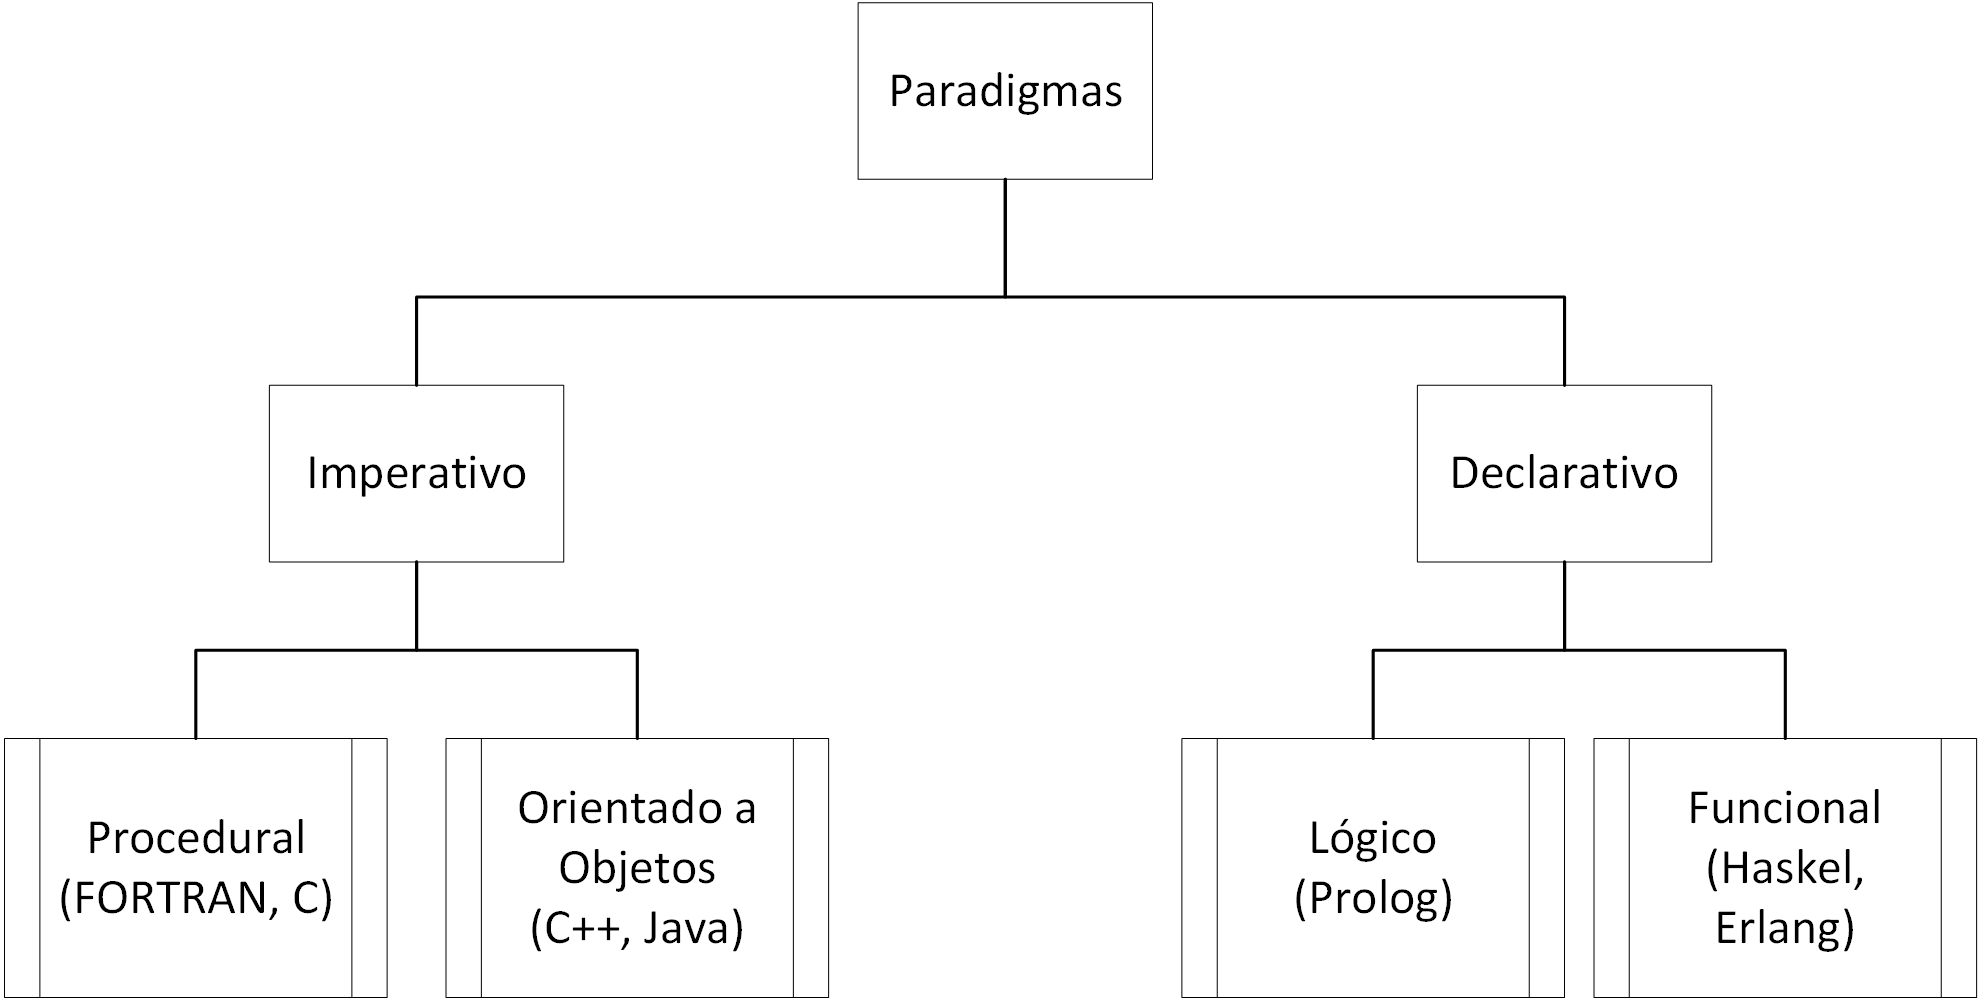
\includegraphics[scale=0.7]{Figuras/Ilustrations-Paradigms.png}
	\caption{Paradigmas de programação}
	\label{fig:Ilustrations-Paradigms}
	\end{figure}


Para a modelagem de problemas de inteligência artificial, geralmente são escolhidas linguagens que pertencem aos paradigmas funcionais, porém, tais linguagens possuem mais limitações que as pertencentes ao paradigma imperativo, seja este limite em relação ao controle sobre o sistema ou aos dados. Este é um dos motivos de se ter escolhido uma linguagem pertencente ao paradigma imperativo (em sua essência) para o desenvolvimento deste trabalho. Como pode-se ver na Figura \ref{fig:Ilustrations-Paradigms} o paradigma imperativo divide-se em dois principais sub paradigmas, o procedural e o orientado a objetos (paradigma escolhido como melhoria para o desenvolvimento). 

A linguagem de programação escolhida para o desenvolvimento do ICA pertence ao paradigma de programação imperativo orientado a objetos em sua maior parte, porém algumas de suas características se encaixam nas funcionalidades do paradigma declarativo funcional, que são funcionalidades como delegados (\emph{Delegate} - os quais permitem que funções sejam tratadas como objetos de primeira ordem, o que nada mais é do que um tipo seguro de ponteiro de função), inferência de tipo (que faz dedução automática de um tipo de dados), funções anônimas (ou abstrações lambdas), linguagem de consulta integrada (Language Integrated Query - LINQ), entre outros. Estes recursos são capazes de otimizar e imitar algumas das características utilizadas pelo paradigma declarativo funcional dentro de uma linguagem imperativa orientada a objetos. Assim, pode-se dizer que a linguagem é multi paradigmas, pois possui características de orientação a objetos, que permite tratar os campos de dados como objetos manipuláveis através de métodos pré-definidos, e permitindo também que a implementação faça o uso dos seus quatro conceitos mais importantes: abstração, encapsulamento, polimorfismo e herança, além de usufruir dos conceitos que não fazem parte paradigma imperativo, que também estão presentes na linguagem. 

O algoritmo do ICA foi desenvolvido neste trabalho utilizando a linguagem de programação C\#. Como descrito acima, esta linguagem multi paradigmas permite o uso dos conceitos de orientação a objetos, que possibilitam uma forma diferente de organizar o problema. Tendo em mente que para se desenvolver uma solução que resolva o problema proposto, será necessário efetuar diversos testes com diversos modelos. A aplicação dos conceitos de orientação a objetos será imprescindível para organizar e manter o desenvolvimento de forma ágil e resiliente. A modelagem do ICA orientado a objetos foi particionado em 4 etapas básicas, na qual cada uma referencia a um dos 4 pilares da Orientação a Objetos.

Primeiramente, foi pensado em como separar os elementos básicos do ICA em objetos de forma que tais objetos pudessem ser caracterizados de forma a ter uma identidade única, seus próprios métodos e propriedades dentro do escopo em questão, abstraindo a concepção do ICA para algo mais tangível como na separação em objetos que podem ser descritos por classes (inclusive interfaces e classes abstratas). Assim, foram criadas duas classes, uma classe abstrata e uma interface, sendo elas:
\begin{itemize}
\item Classe \emph{ Country }
\item Classe \emph{ImperialistCompetition  }
\item Interface \emph{IFitness}
\item Classe Abstrata \emph{ StopCondition}
\end{itemize}

A classe \emph{Country} (Figura \ref{fig:ClassesICA-Country})  representa um país do ICA, sendo este colônia ou império, e é semelhante a um indivíduo no GA. O país possui o conjunto de atributos que serão usados pela função de avaliação de modo que esta função de avaliação calcule um custo para este país, sendo este valor de custo armazenado na própria classe. Esta classe ainda armazena atributos que definem se o país é um país imperialista ou se ele é uma colônia. Logo, para que se possa manusear melhor o país, independente de sua posição política, existe um valor que representa dois estados, dependendo do que o país possa ser, colônia ou império. Se este país for uma colônia, este valor representará o numero do império a que este país pertence. Se este país for um império, este valor será o índice do vetor de impérios ordenados por custos presente na classe ImperialistCompetition descrita logo abaixo.

Durante o desenvolvimento foi pensado que poderiam ser criadas mais duas classes, sendo estas a classe Colônia e a classe Imperialista, que derivariam da classe \emph{Country}, porém não foram criadas por dois motivos: (1) A concepção de uma classe Colônia e uma classe Imperialista que derivassem da classe \emph{Country} não teriam nem propriedades e nem métodos que as diferenciassem da classe, sendo estas diferentes apenas suas identidades (OBS: a classe imperialista até poderia possuir um vetor para as colônias que controla, mas seria redundante e aumentaria a complexidade no controle das operações efetuadas pelo ICA). (2) O segundo motivo é referente ao impacto da implementação destas duas classes, que necessitaria de muito mais lógica para manuseio dos objetos, sendo que o foco não é implementar uma abstração tão afundo da ideia original, mas sim uma implementação de baixa complexidade, que faça com que o sistema seja simples de ser mantido e testado. 

\begin{figure}[h]
	\centering	
	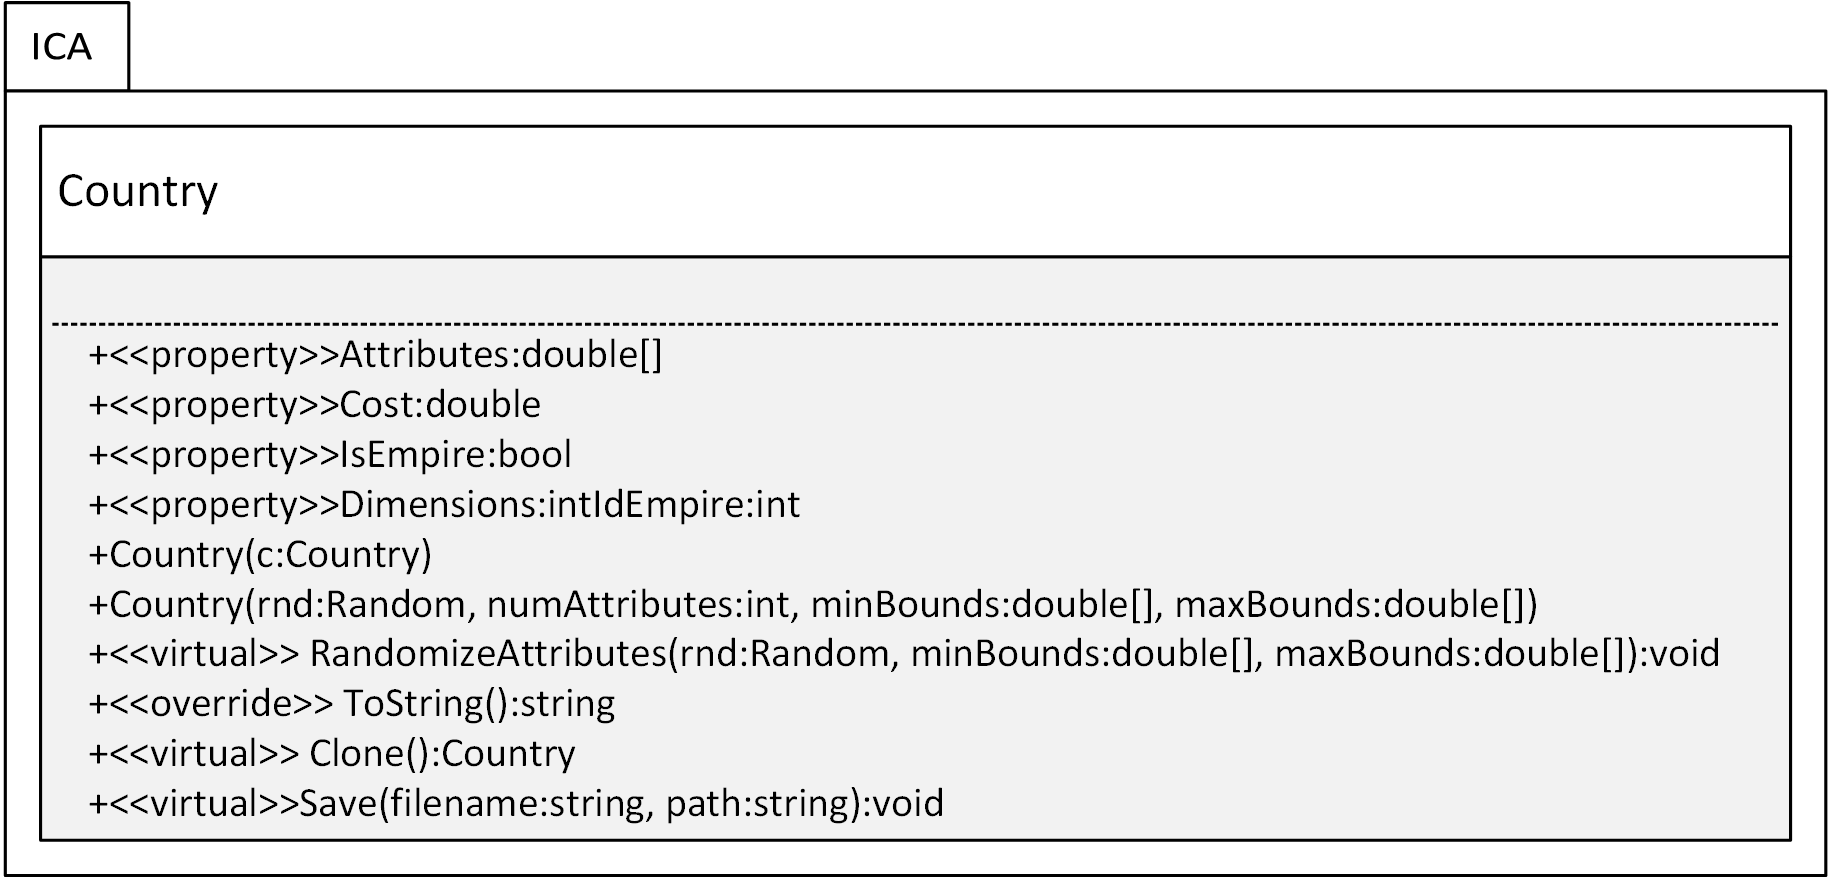
\includegraphics[scale=1]{Figuras/ClassesICA-Country.png}
	\caption{Classe Country}
	\label{fig:ClassesICA-Country}
	\end{figure}

Para completar a modelagem da classe \emph{Country}, foram adicionados alguns métodos essenciais para o funcionamento genérico do ICA. Dois destes métodos são construtores para a classe, no qual o primeiro recebe como parâmetro um outro objeto do tipo \emph{Country} e inicializa seus valores fazendo uma cópia direta de todos os atributos do parâmetro, o segundo construtor inicializa todos os seus valores com valores padrão da linguagem, porém recebe diversos parâmetros, nos quais são basicamente usados para chamar o método \emph{RandomizeAttributes} logo após a inicialização dos valores da classe. Dentre os quatro métodos restantes o método \emph{ToString} é o mais simples, apenas retornando uma cadeia de caracteres formatada dos valores da classe, o método \emph{Clone} faz uma cópia do objeto em questão usando o primeiro construtor, o método \emph{Save} grava em um arquivo de texto com os dados do objeto, e por fim, o método \emph{RandomizeAttributes} faz uma randomização dentro dos valores \emph{minBounds} e \emph{maxBounds} para todos os atributos do indivíduo. 


Nota-se ainda que os métodos \emph{RandomizeAttributes} e \emph{Clone} são virtuais, isto indica que quando a classe \emph{Country} for derivada (usando o conceito de herança), estes métodos poderão ser substituídos por novos métodos com uma lógica diferenciada (OBS: o construtor da classe também pode ser sobrescrito e ter sua lógica alterada em um cenário de extensão da classe \emph{Country}). O fato de poder se criar uma classe tomando como base a classe \emph{Country} e mesmo assim o ICA continuar funcionando é devido à aplicação do conceito de polimorfismo aplicado na modelagem da aplicação. Neste caso, quando se implementa uma classe\emph{ Country} estendida, o ICA não é responsável por instanciar a lista de países, esta responsabilidade é do método \emph{GenerateCountries}, que deve ser implementado por classes derivadas da interface \emph{IFitness} (descrita logo abaixo). Assim, na classe \emph{Country}, foram abordados todos os quatro conceitos essenciais de orientação a objetos, mantendo uma grande flexibilidade para a utilização genérica do ICA.    

A classe \emph{ImperialistCompetition} será abordada por último, pois é nela que todos os outros componentes são interligados e é necessário que os demais componentes estejam bem definidos. Então, continuando com a interface \emph{IFitness}, que é responsável por fazer com que os objetos que venha a implementá-la, obrigatoriamente tenham os métodos de interface implementados. Como pode-se observar na Figura \ref{fig:ClassesICA-IFitness}, de todos os métodos, o mais importante é o método \emph{Eval} e em seguida o método \emph{GenerateCountries}, descritos mais detalhadamente logo abaixo.


\begin{figure}[h]
	\centering	
	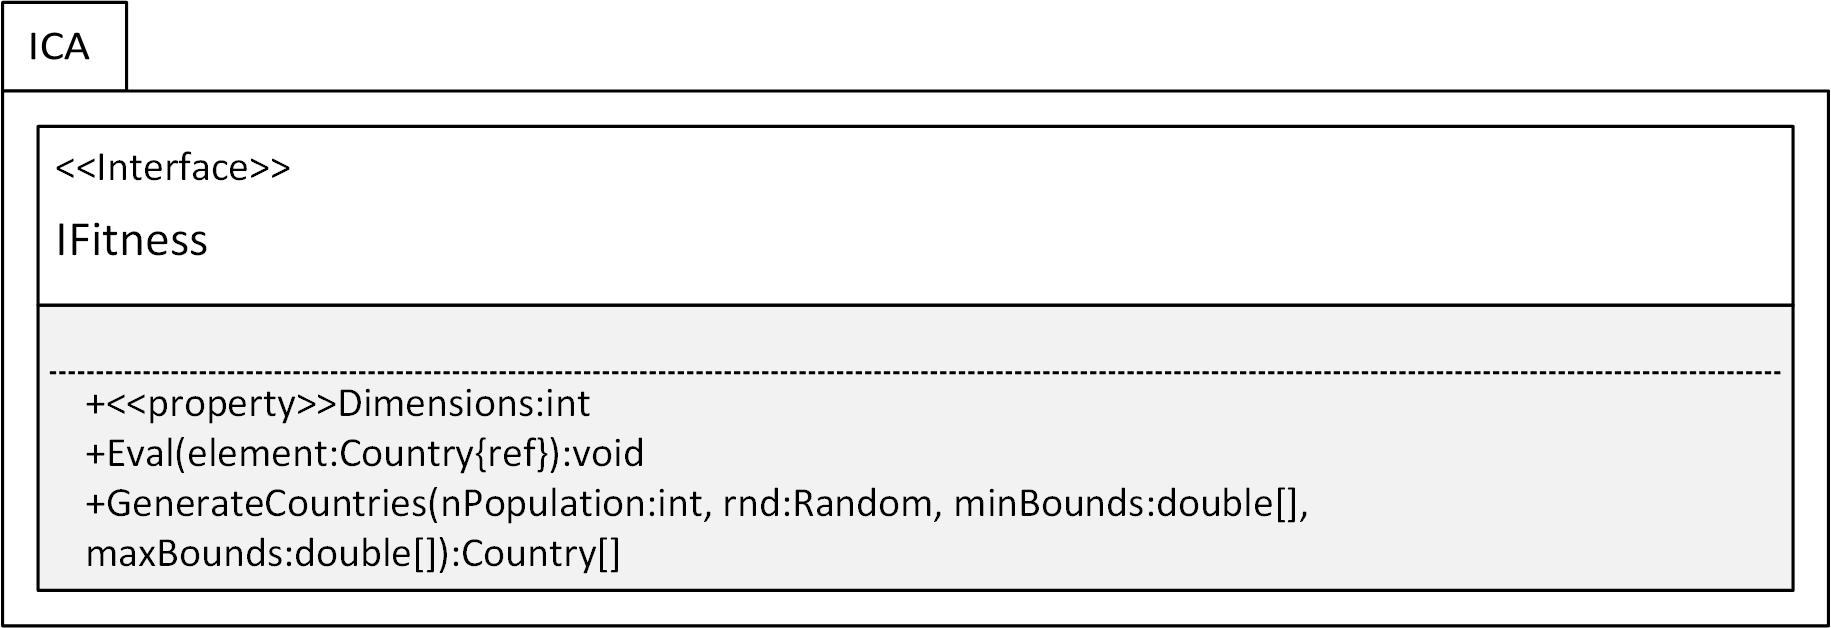
\includegraphics[scale=1]{Figuras/ClassesICA-IFitness.png}
	\caption{Interface IFitness}
	\label{fig:ClassesICA-IFitness}
	\end{figure}


O método \emph{Eval} é o mais importante, ele representa a própria função de avaliação do problema em questão e é o principal fator que levou a criação desta interface. É neste método que ocorrem os cálculos para a avaliação de cada país e consequentemente a atribuição do valor do custo calculado a cada país em questão. É essencial que seja passado como parâmetro a referência de um país para que o custo seja calculado a partir dos valores deste, e em seguida já atribuir o valor do custo a este país passado por referência. Assim, qualquer alteração ao país, que ocorra dentro da função \emph{Eval} será persistida para o objeto no escopo da classe \emph{ImperialistCompetition}, vista mais adiante que é a responsável por fazer as chamadas de avaliação dos países, desta forma evita-se múltiplas trocas de mensagens e simplifica-se o funcionamento, tanto para o processamento serial, quanto para paralela.
 
Na sequência, o segundo método, \emph{GenerateCountries}, é quem define a construção da lista de países para que o ICA possa iniciar sua execução, a lista de países pode ser iniciada normalmente, gerando-se uma lista e inicializando seus elementos, porém, a grande vantagem de se ter este método de forma explícita e obrigatória para cada problema a ser implementado é referente a liberdade de poder inicializar alguns países (ou todos) em posições privilegiadas, ou seja, se existir algum pré processamento nos dados, pode-se iniciar os países e seus atributos de forma que estes estejam próximos da solução ótima sem que se precise limitar o espaço de busca. Os parâmetros de entrada para este método são:
\begin{itemize}
\item \emph{nPopulation} - valor que representa a quantidade de países a serem criados,
\item \emph{rnd} - um objeto do tipo \emph{Random} para que a aleatorização inicial seja efetuada sem que ocorram problemas com a paralelização (discutidos no tópico sobre Paralelização),
\item \emph{maxBounds} e \emph{minBounds} -  que são as duas listas de valores representando os limites superior e inferior respectivamente para cada dimensão do problema.
\end{itemize}

Nota-se ainda uma propriedade chamada \emph{Dimensions} na interface, sendo que esta propriedade é responsável por definir o número de dimensões do problema em questão. Como visto anteriormente o valor de dimensão é que definirá o tamanho do vetor de atributos dos países, sendo este valor muito usado pelo ICA. A inserção desta propriedade para definir este valor na interface implica que a classe responsável pelo controle do algoritmo não precisa se preocupar em inicializar tal valor (pois, na maioria dos casos, seu valor dependerá da modelagem do problema). Cada problema no ICA deve ser modelado de forma que possa ter suas soluções na forma de um vetor de valores, no caso do ICA tais valores são números de ponto flutuante, sendo o número de elementos deste vetor o número de dimensões do problema.

Por fim, percebe-se que a interface \emph{IFitness} é a responsável por encapsular a lógica do problema a ser otimizado através da implementação de seus membros em uma classe separada para cada problema. Assim, cria-se um nível de abstração que separa o funcionamento do algoritmo da implementação/avaliação do problema, sendo que a classe \emph{ImperialistCompetition} deve obrigatoriamente obter os valores necessários para sua execução (Lista de países, número de dimensões do problema e chamada da função de avaliação de um país) a partir de uma implementação da interface \emph{IFitness}, porém não precisa ter informação alguma sobre como a acontece a geração da lista de países, como avaliação de um dado país ocorre ou como se define o valor de dimensões do problema etc.. Assim, quando se implementa uma função de avaliação para um dado problema, na maioria das vezes existe a necessidade de manter variáveis do problema que não fazem parte diretamente da solução, mas sim do modelo do problema. Estes valores devem estar inseridos na classe que implementa o problema, para que o ICA não precise ter suas funcionalidades principais alteradas, mantendo a aplicação genérica a qualquer problema deve-se implementar a interface \emph{IFitness} e seus métodos com o foco no problema em questão. Desta forma ICA se mantém genérico a qualquer solução, sendo que qualquer classe que implemente um problema diferente seja polimórfica, ou seja, independente do problema em questão, o ICA apenas utilizará os métodos e propriedades expostos pela interface \emph{IFitness}, não tendo contato algum com os demais elementos da modelagem do problema.

	Na metodologia do ICA foi mostrado que podem haver diversas formas de convergir um problema, porém a solução ótima geralmente se apresenta quando existe apenas um país imperialista, e este imperialista possui todas as colônias geradas inicialmente, de forma que tais colônias estejam na mesma posição em que o país imperialista se encontra. Durante a execução de alguns problemas, notou-se que a convergência para apenas um país pode levar muito tempo, ou também que pode-se atingir uma solução aceitável mesmo ela não sendo pertencente ao cenário ótimo de convergência do ICA. Assim, para que o ICA possa gerenciar diversas condições de parada para um dado problema foi pensada uma abstração que permite extrair apenas a lógica das condições de parada para fora do ICA.

A Figura \ref{fig:ClassesICA-StopCondition} apresenta a classe \emph{StopCondition}, que define como foi modelada a abstração das condições de parada. Uma condição de parada deve implementar esta classe e definir as regras de parada dentro do método \emph{VerifyBreak}, que é chamado sempre que se inicia um ciclo (ou década, contextualizando para o ICA) no algoritmo. Observa-se que diversos parâmetros são passados para este método, assim, as condições de parada mais comuns podem ser implementadas e adicionadas no ICA. Ainda existem duas propriedades na classe abstrata, a primeira, é usada apenas para definir o nome da condição de parada, para fins de análise. Já a segunda, é usada exclusivamente pelo ICA para gerenciar uma lista de diversas condições de parada que possam estar sendo verificadas em sequencia. Note que tal propriedade é pública, porém possui o método \emph{set} como interno (definido pela palavra chave \emph{Internal}), o que significa que apenas a própria instância pode alterar o valor, mas qualquer um pode lê-lo (pois o seu método \emph{get} continua público).
 
\begin{figure}[h]
	\centering	
	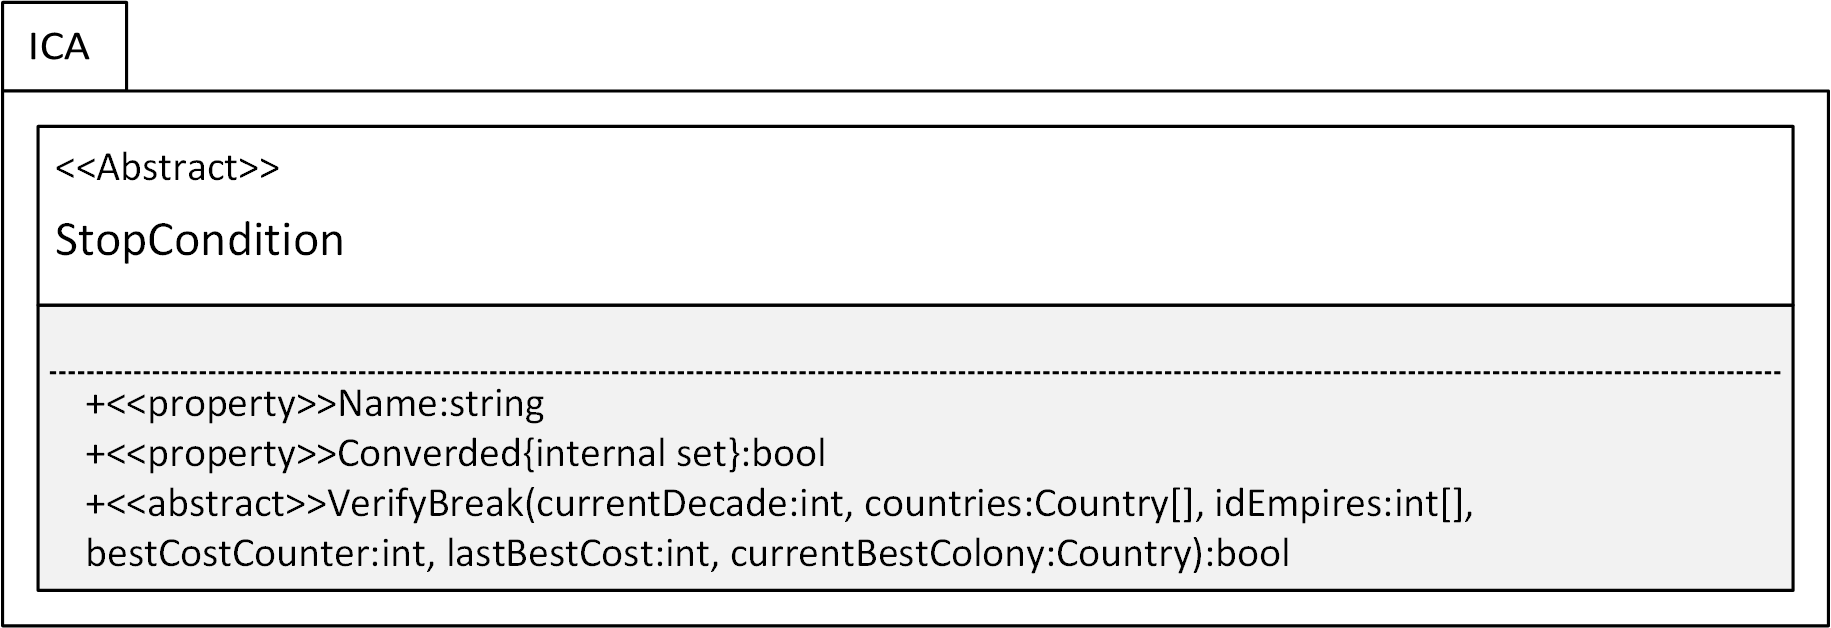
\includegraphics[scale=1]{Figuras/ClassesICA-StopCondition.png}
	\caption{Classe Abstrata StopCondition}
	\label{fig:ClassesICA-StopCondition}
	\end{figure}

A Figura\ref{fig:ClassesICA-StopConditionsImplements} define as condições de parada:
\begin{itemize}
\item Número máximo de décadas - que força parada da evolução do ICA quando um valor de iterações (décadas) for atingido. 
\item Estagnação por década - que força parada da evolução do ICA quando o valor do melhor custo da solução não se alterar durante um número de ciclos (décadas) estipulado.
\item Estagnação por porcentagem de custo - que força a parada da evolução do ICA quando o valor do melhor custo subtraído do melhor custo anterior  se manter dentro de uma variação percentual durante um número de ciclos (décadas) estipulado.
\end{itemize}
Tais condições de parada foram implementadas e inseridas na rotina de iteração do ICA, para que este possa convergir mais rapidamente para uma solução aceitável. A utilização destas condições de parada é configurável e portanto pode-se utilizar a condição padrão citada na metodologia, que apenas irá parar o algoritmo quando todas as colônias estiverem sob o poder de apenas um império de tal forma que suas posições sejam as mesmas.

\begin{figure}[h]
	\centering	
	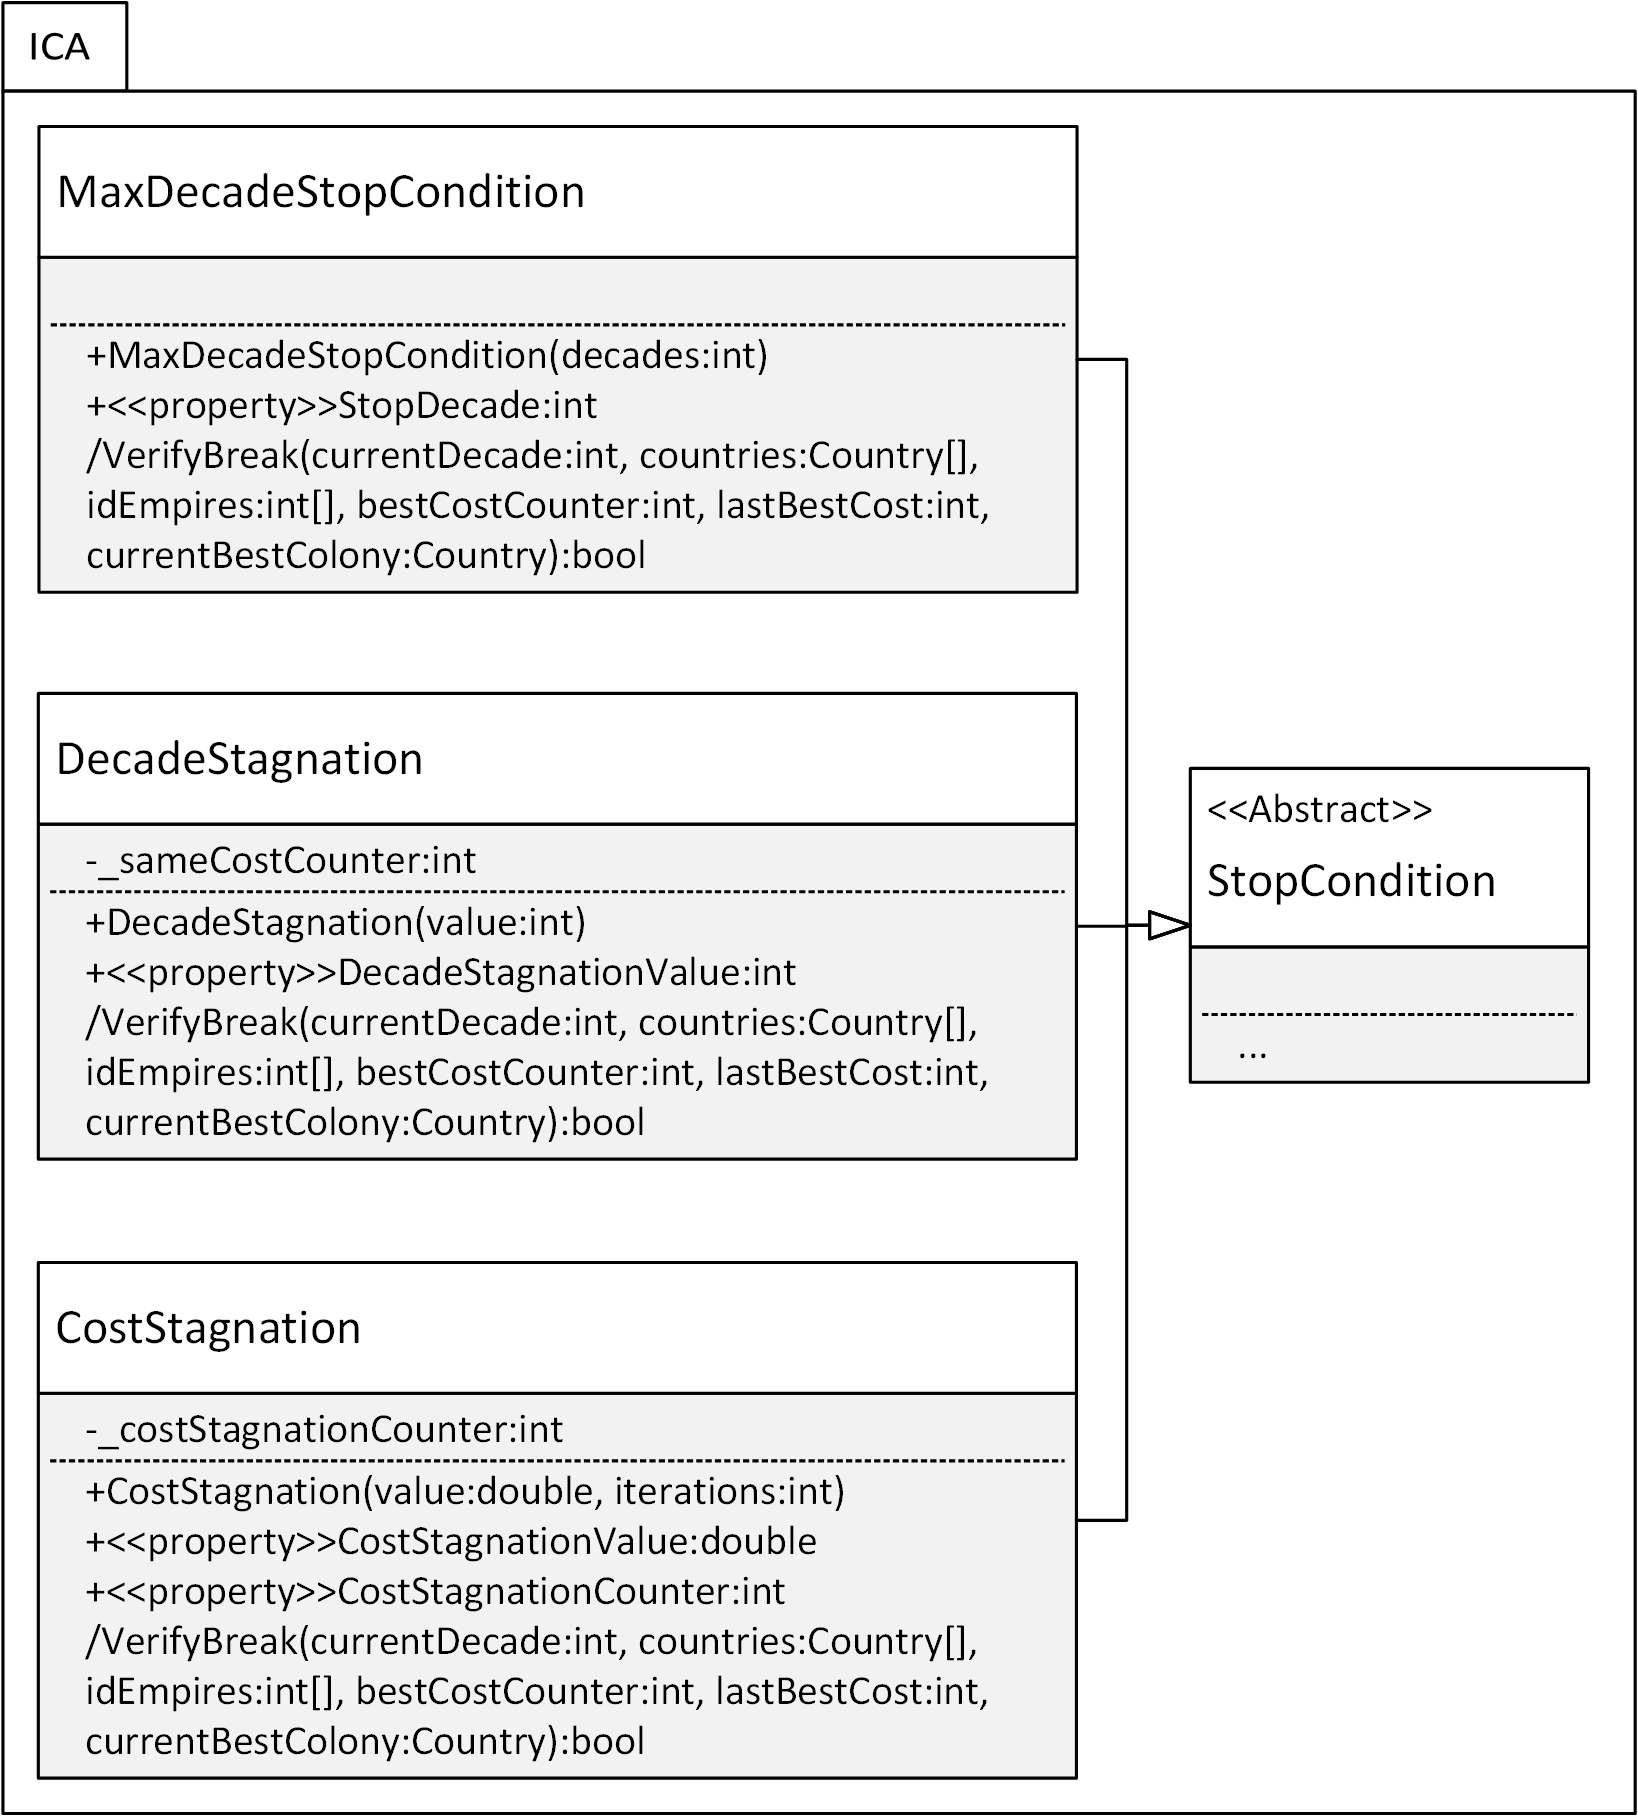
\includegraphics[scale=1]{Figuras/ClassesICA-StopConditionsImplements.png}
	\caption{Implementação das condições de parada}
	\label{fig:ClassesICA-StopConditionsImplements}
	\end{figure}

Por fim, a classe \emph{ImperialistCompetition} controla toda a competição imperialista, desde a inicialização dos países até o término da competição. Ela é a implementação do fluxograma do ICA apresentado na metodologia, com alterações para adição de novos recursos como processamento paralelo e orientação a objetos, tornando o ICA genérico a qualquer problema. Sendo assim, todos os elementos, lógicas, condições e ideias descritas anteriormente no fluxograma são abstraídas de modo que esta classe processe a competição imperialista idealizada, usando de seus métodos e propriedades em conjunto com os demais elementos modelados (classe \emph{Country}, classe abstrata \emph{StopCondition} e interface \emph{IFitness}).

A Figura \ref{fig:ClassesICA-ImperialistCompetition} representa apenas a classe em questão, destacando em tom mais claros, na área onde se situam os membros da classe, elementos que fazem alguma ligação de relacionamento, seja esta uma associação, agregação ou composição, que podem ser melhor visualizados na Figura \ref{fig:ClassesICA-ICAResumed}, que por sua vez representa toda a implementação do ICA orientado a objetos e como os elementos se interagem, porém omite as propriedades e métodos das classes para que melhor visualização. Nota-se também na imagem que descreve a classe \emph{ImperialistCompetition} com suas propriedades e métodos, que para facilitar o entendimento foram adicionados comentários (texto entre \emph{'/*'} e \emph{'*/'}) que regionalizam as propriedades e métodos usados nesta classe, já que ela é a responsável por implementar, além dos conceitos básicos do ICA, todas as alterações estruturais e de otimização.

Como a classe \emph{ImperialistCompetition} tem uma quantidade muito grande de propriedades e métodos, estes serão melhores detalhados no anexo, e neste texto, apenas serão detalhados os processos principais ao funcionamento da classe e como os elementos são usados para executar o processo evolutivo do ICA.

Uma das partes mais complexas do ICA é o preparo para o processo evolutivo, referindo-se a etapa de inicialização dos países presente no do fluxograma do ICA apresentado na metodologia pela figura \ref{fig:Fluxograms-ICACanonic}, países estes, que por sua vez, devem estar separados em impérios antes que o este processo evolutivo de fato comece. Quando se instancia a classe \emph{ImperialistCompetition}, ainda não são efetuadas as tarefas responsáveis por esta etapa de inicialização dos países, pois ainda existirão valores que devem ser configurados, como a adição de um objeto do tipo \emph{IFitness} através da propriedade \emph{Fitness}, e definição dos limites do problema, sejam estes chamados pelo método \emph{InitializeBounds} ou adicionados manualmente nas propriedades \emph{MinBounds} e \emph{MaxBounds}.

A partir do momento em que todos os valores estão configurados apropriadamente, pode-se executar o método \emph{Run()}, que é dividido em duas etapas principais, onde uma delas consiste na etapa de inicialização dos países, e refere-se diretamente à primeira atividade presente no fluxograma do ICA apresentado na metodologia pela figura \ref{fig:Fluxograms-ICACanonic}, e a segunda consiste no conjunto formado por todos os elementos presentes no \emph{loop} principal, definido como processo evolutivo, referentes ao restante das atividades presentes no fluxograma.


 \begin{figure}[h]
	\centering	
	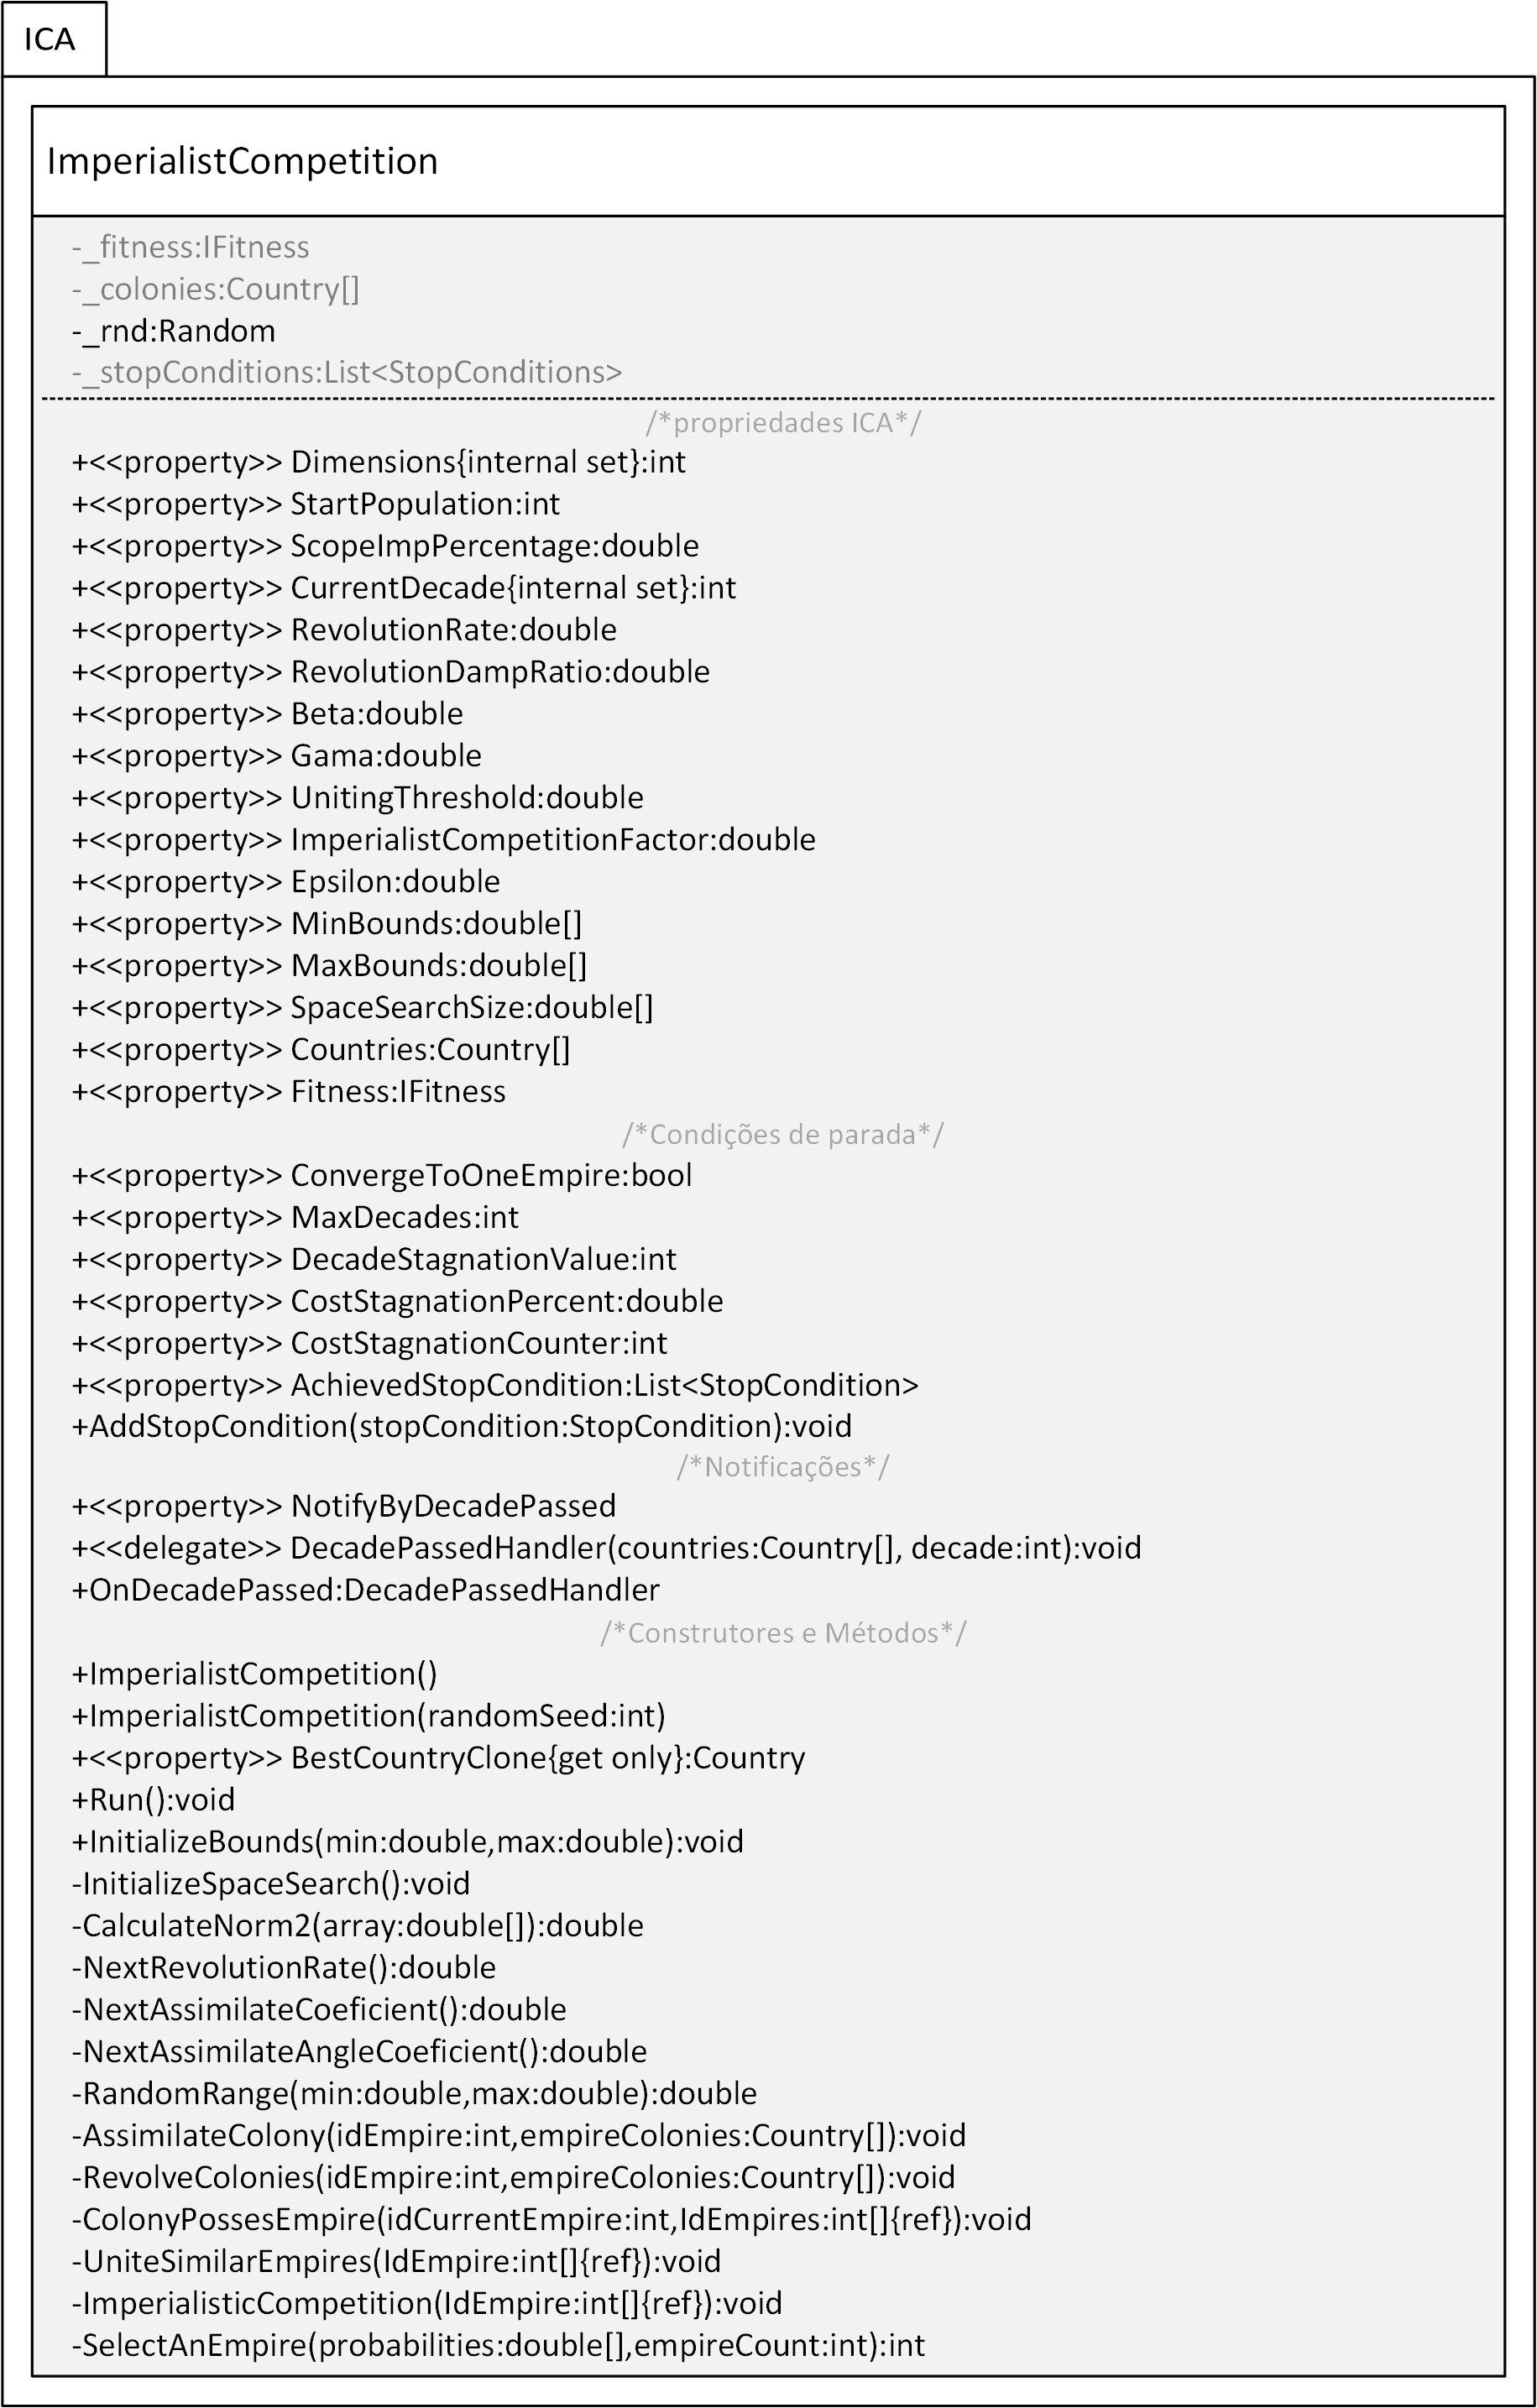
\includegraphics[scale=0.8]{Figuras/ClassesICA-ImperialistCompetition.png}
	\caption{Classe ImperialistCompetition}
	\label{fig:ClassesICA-ImperialistCompetition}
	\end{figure}
    
Então, assim que o método \emph{Run()} é chamado, inicia-se a etapa de inicialização dos países, que por sua vez tem como atividade inicial, instanciar as condições de parada padrões, sendo elas:

\begin{itemize}
\item Condição de parada por número máximo de décadas; 
\item Condição de parada por estagnação de custo idêntico durante as décadas; 
\item Condição de parada por estagnação de custo em um intervalo durante as décadas, do ICA. 
\end{itemize}

Observe ainda, que o relacionamento apresentado na Figura: Diagrama de classes ICA é de agregação para estas três condições de parada, pois é nesta classe que elas são criadas e mantidas, porém o ciclo de vida destes objetos podem se estender para além do deste objeto, uma vez que existe a propriedade \emph{AchievedStopCondition}, que expõe tais objetos publicamente de forma que estes possam ser referenciados fora desta classe, caso contrário, o relacionamento em questão deveria ser de composição.

\begin{figure}[h]
	\centering	
	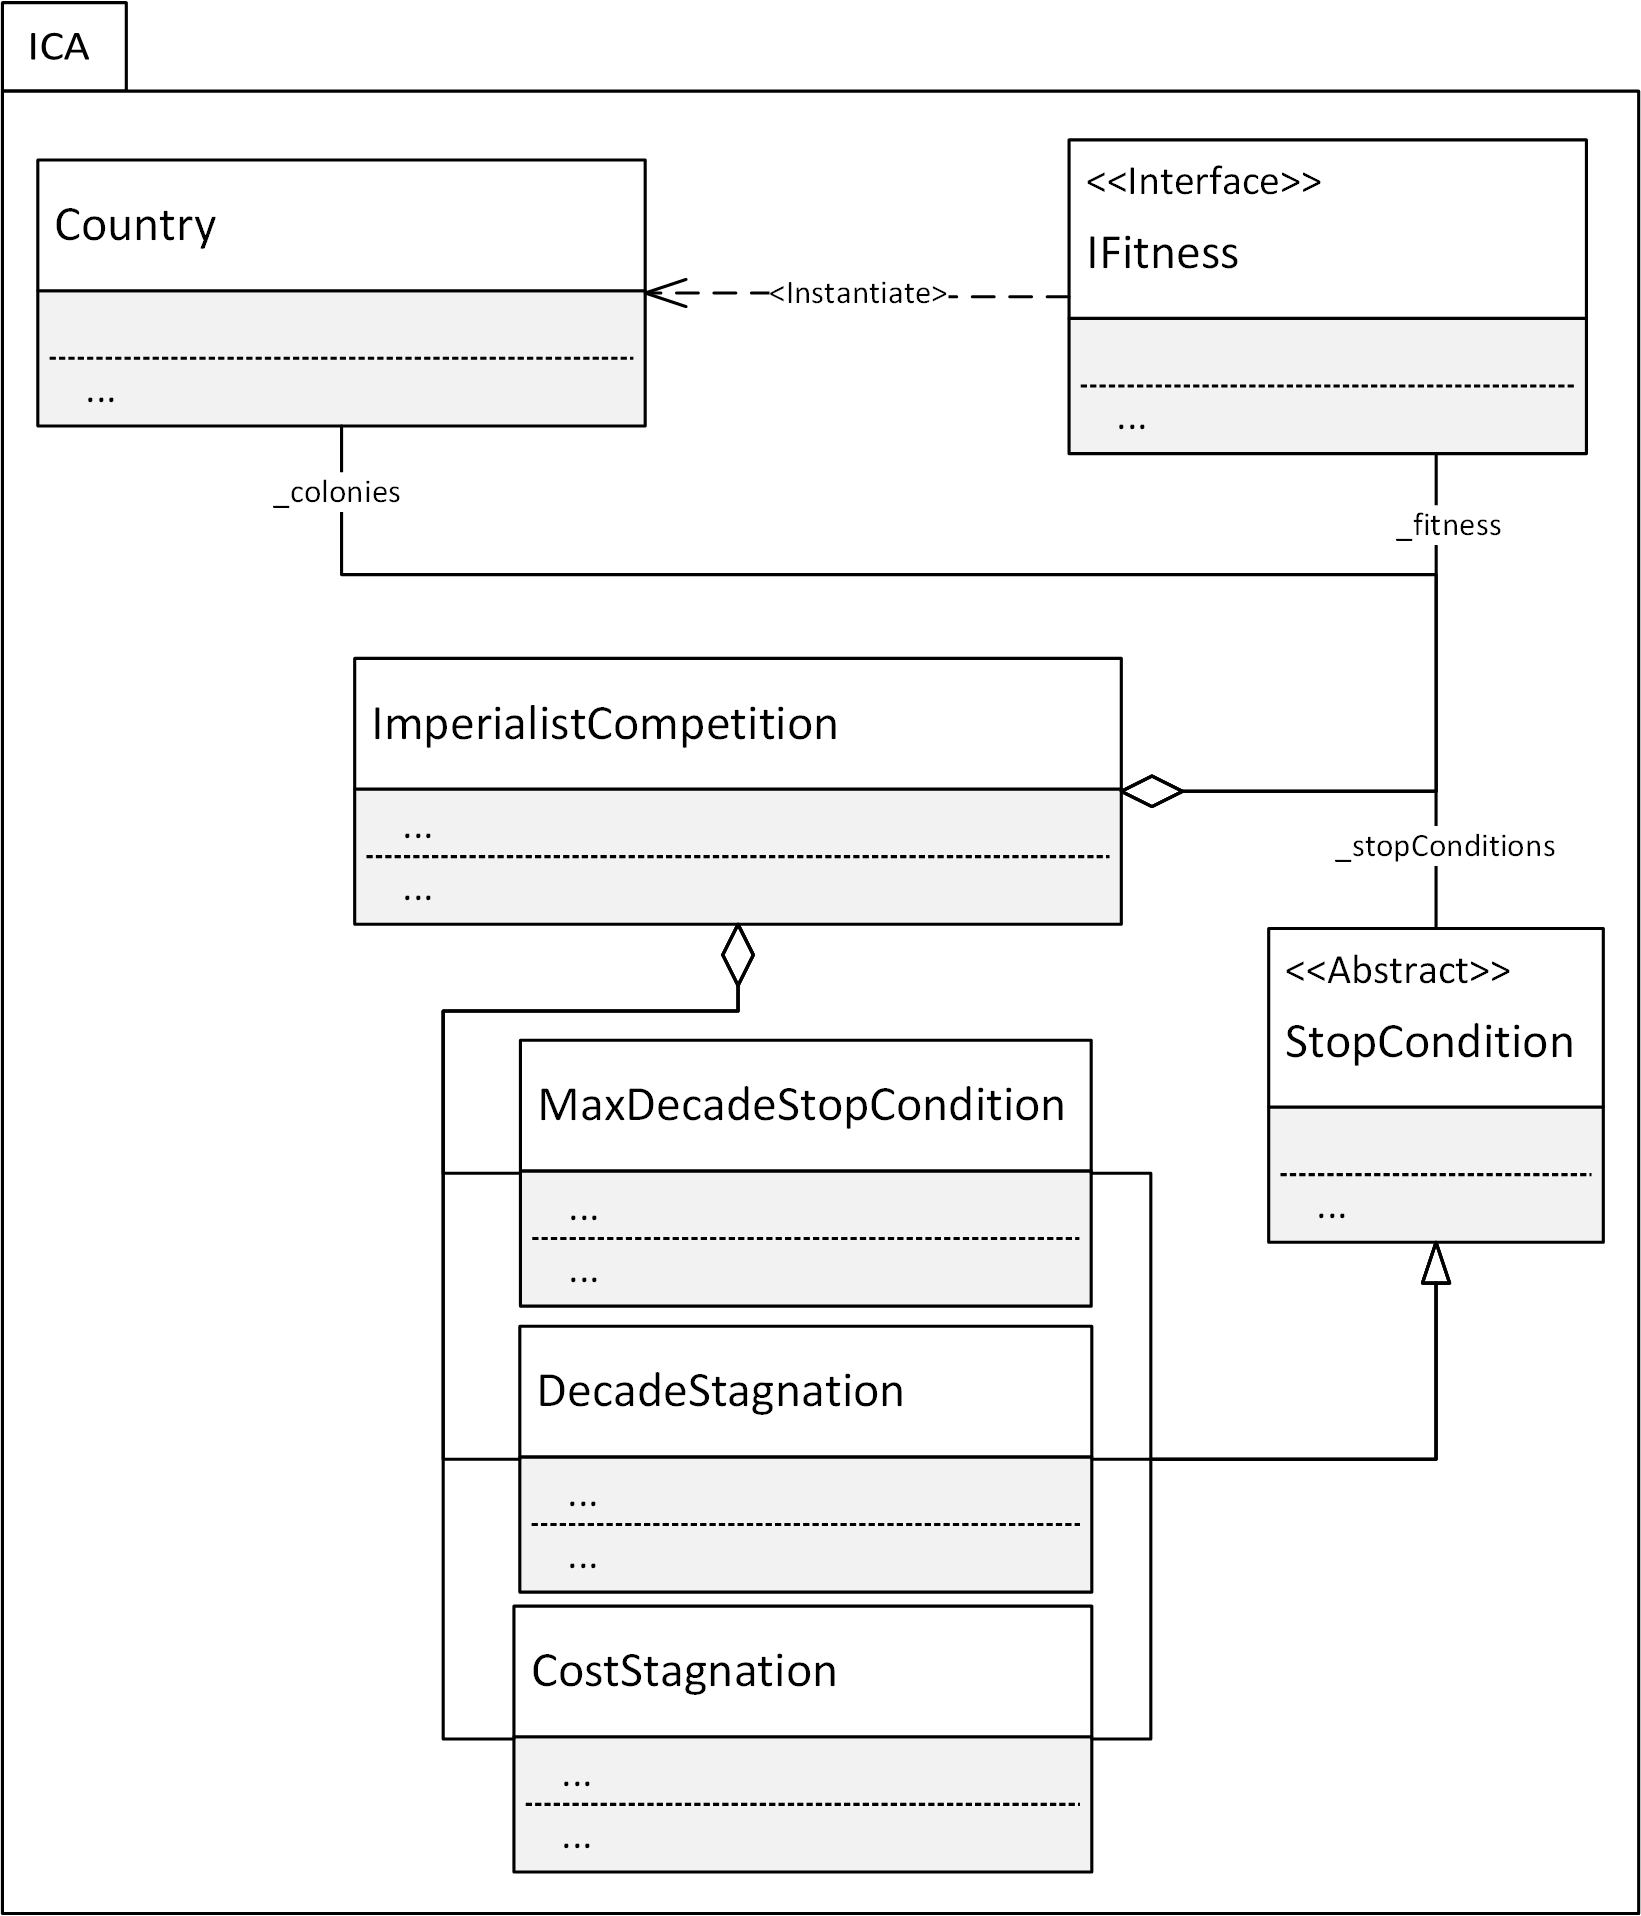
\includegraphics[scale=0.9]{Figuras/ClassesICA-ICAResumed.png}
	\caption{Diagrama de classes resumido do ICA }
	\label{fig:ClassesICA-ICAResumed}
	\end{figure}
    
Em seguida, inicializam-se os valores constantes ou de cálculo simples, como tamanho do espaço de busca (\emph{SpaceSearchSize}, pelo método \emph{InitializeSpaceSearch}), número populacional (\emph{nPop}), número de impérios (\emph{nImp}) e número de colônias (\emph{nCol}). Então, com estes valores já estipulados, faz-se uma chamada ao método \emph{GenerateCountries} do objeto \emph{Fitness} para que seja criado o vetor de países que será usado no processo evolutivo.

Mesmo tendo em mão este vetor com os países já inicializados para o problema em questão, não se pode dar a etapa de inicialização como terminada, pois ainda não foram gerados os impérios para que se comece a competição imperialista. Então, tão logo que se crie o vetor de países \emph{Countries}, deve-se fazer a chamada para a avaliação do custo de cada país contido nele. Neste caso, o processamento dos custos de cada país é feito pela chamada do método de avaliação \emph{Eval} do objeto \emph{Fitness} para cada país, que é feito de forma paralela, agilizando o processo de avaliação. Observe que deve-se tomar muito cuidado ao implementar o método de avaliação no objeto \emph{Fitness} para que este não compartilhe recursos globais (somente para escrita, pois a leitura de dados pode ser feita paralelamente), de forma que as diversas chamadas a este método de forma paralela não entrem em conflito, prendendo os recursos de processamento apenas para a tarefa em questão.

Com todos os custos calculados, deve-se definir agora, quais dos países serão os países imperialistas, porém, como foi decidido não criar classes extras apenas para separar imperialistas de colônias, foi criado um vetor de índices, que armazena quais os índices presentes no vetor de países \emph{Countries} representam os países imperialistas. Este vetor foi criado utilizando o recurso da linguagem C\# chamado LINQ (Language-Integrated Query), em apenas uma linha de código. Caso este recurso não existisse, seriam necessárias dezenas de linhas de código e chamadas de método para a criação deste vetor de índices. O processo para a criação deste vetor utilizando este recurso é relativamente simples, e envolve a seleção dos índices do vetor de países, ordenado-os e pegando os \emph{nImp} primeiros valores.

Após a criação deste vetor de índices de países imperialistas, deve-se calcular o poder de cada império para que os países restantes sejam distribuídos como colônias dos países imperialistas formando assim os impérios, e para isto, cada país imperialista deve ter um número de colônias que seja proporcional ao seu poder. Para se obter tal valor, gera-se o vetor de valores inteiros \emph{nOfColonies} de tamanho \emph{nImp}, onde cada índice deste vetor representará a quantidade de colônias que cada império terá. 

Para se obter os valores do vetor \emph{nOfColonies} deve-se calcular o poder dos países imperialistas, multiplicá-lo pelo número de colônias \emph{nCol} e por fim arredonda-lo como proposto na equação. Para se obter o valor de poder \emph{pn} de cada país imperialista deve-se calcular inicialmente o custo normalizado para todos os países imperialistas e então atribuir como poder \emph{pn}, de um dado império \emph{n}, a divisão entre seu custo normalizado \emph{C.N.n} pela soma te todos os custos normalizados como demonstrado na metodologia. 

Originalmente o resultado do número de colônias é o arredondamento da multiplicação entre o poder \emph{pn} calculado e o número de colônias \emph{nCol}, porém computacionalmente existe o problema que arredondamentos na computação na verdade são truncamentos, por este ser um ambiente discreto e não contínuo, então é necessária uma etapa extra para verificar se o número total de colônias está correto, e caso não esteja, corrige-se o valor até que a soma dos valores do vetor \emph{nOfColonies} seja igual ao \emph{nCol}, adicionando-se 1 e incrementando o índice do vetor, como pode ser visto na primeira atividade condicional do fluxograma presente na Figura \ref{fig:Fluxograms-RunMethodStart}.

 \begin{figure}[h]
	\centering	
	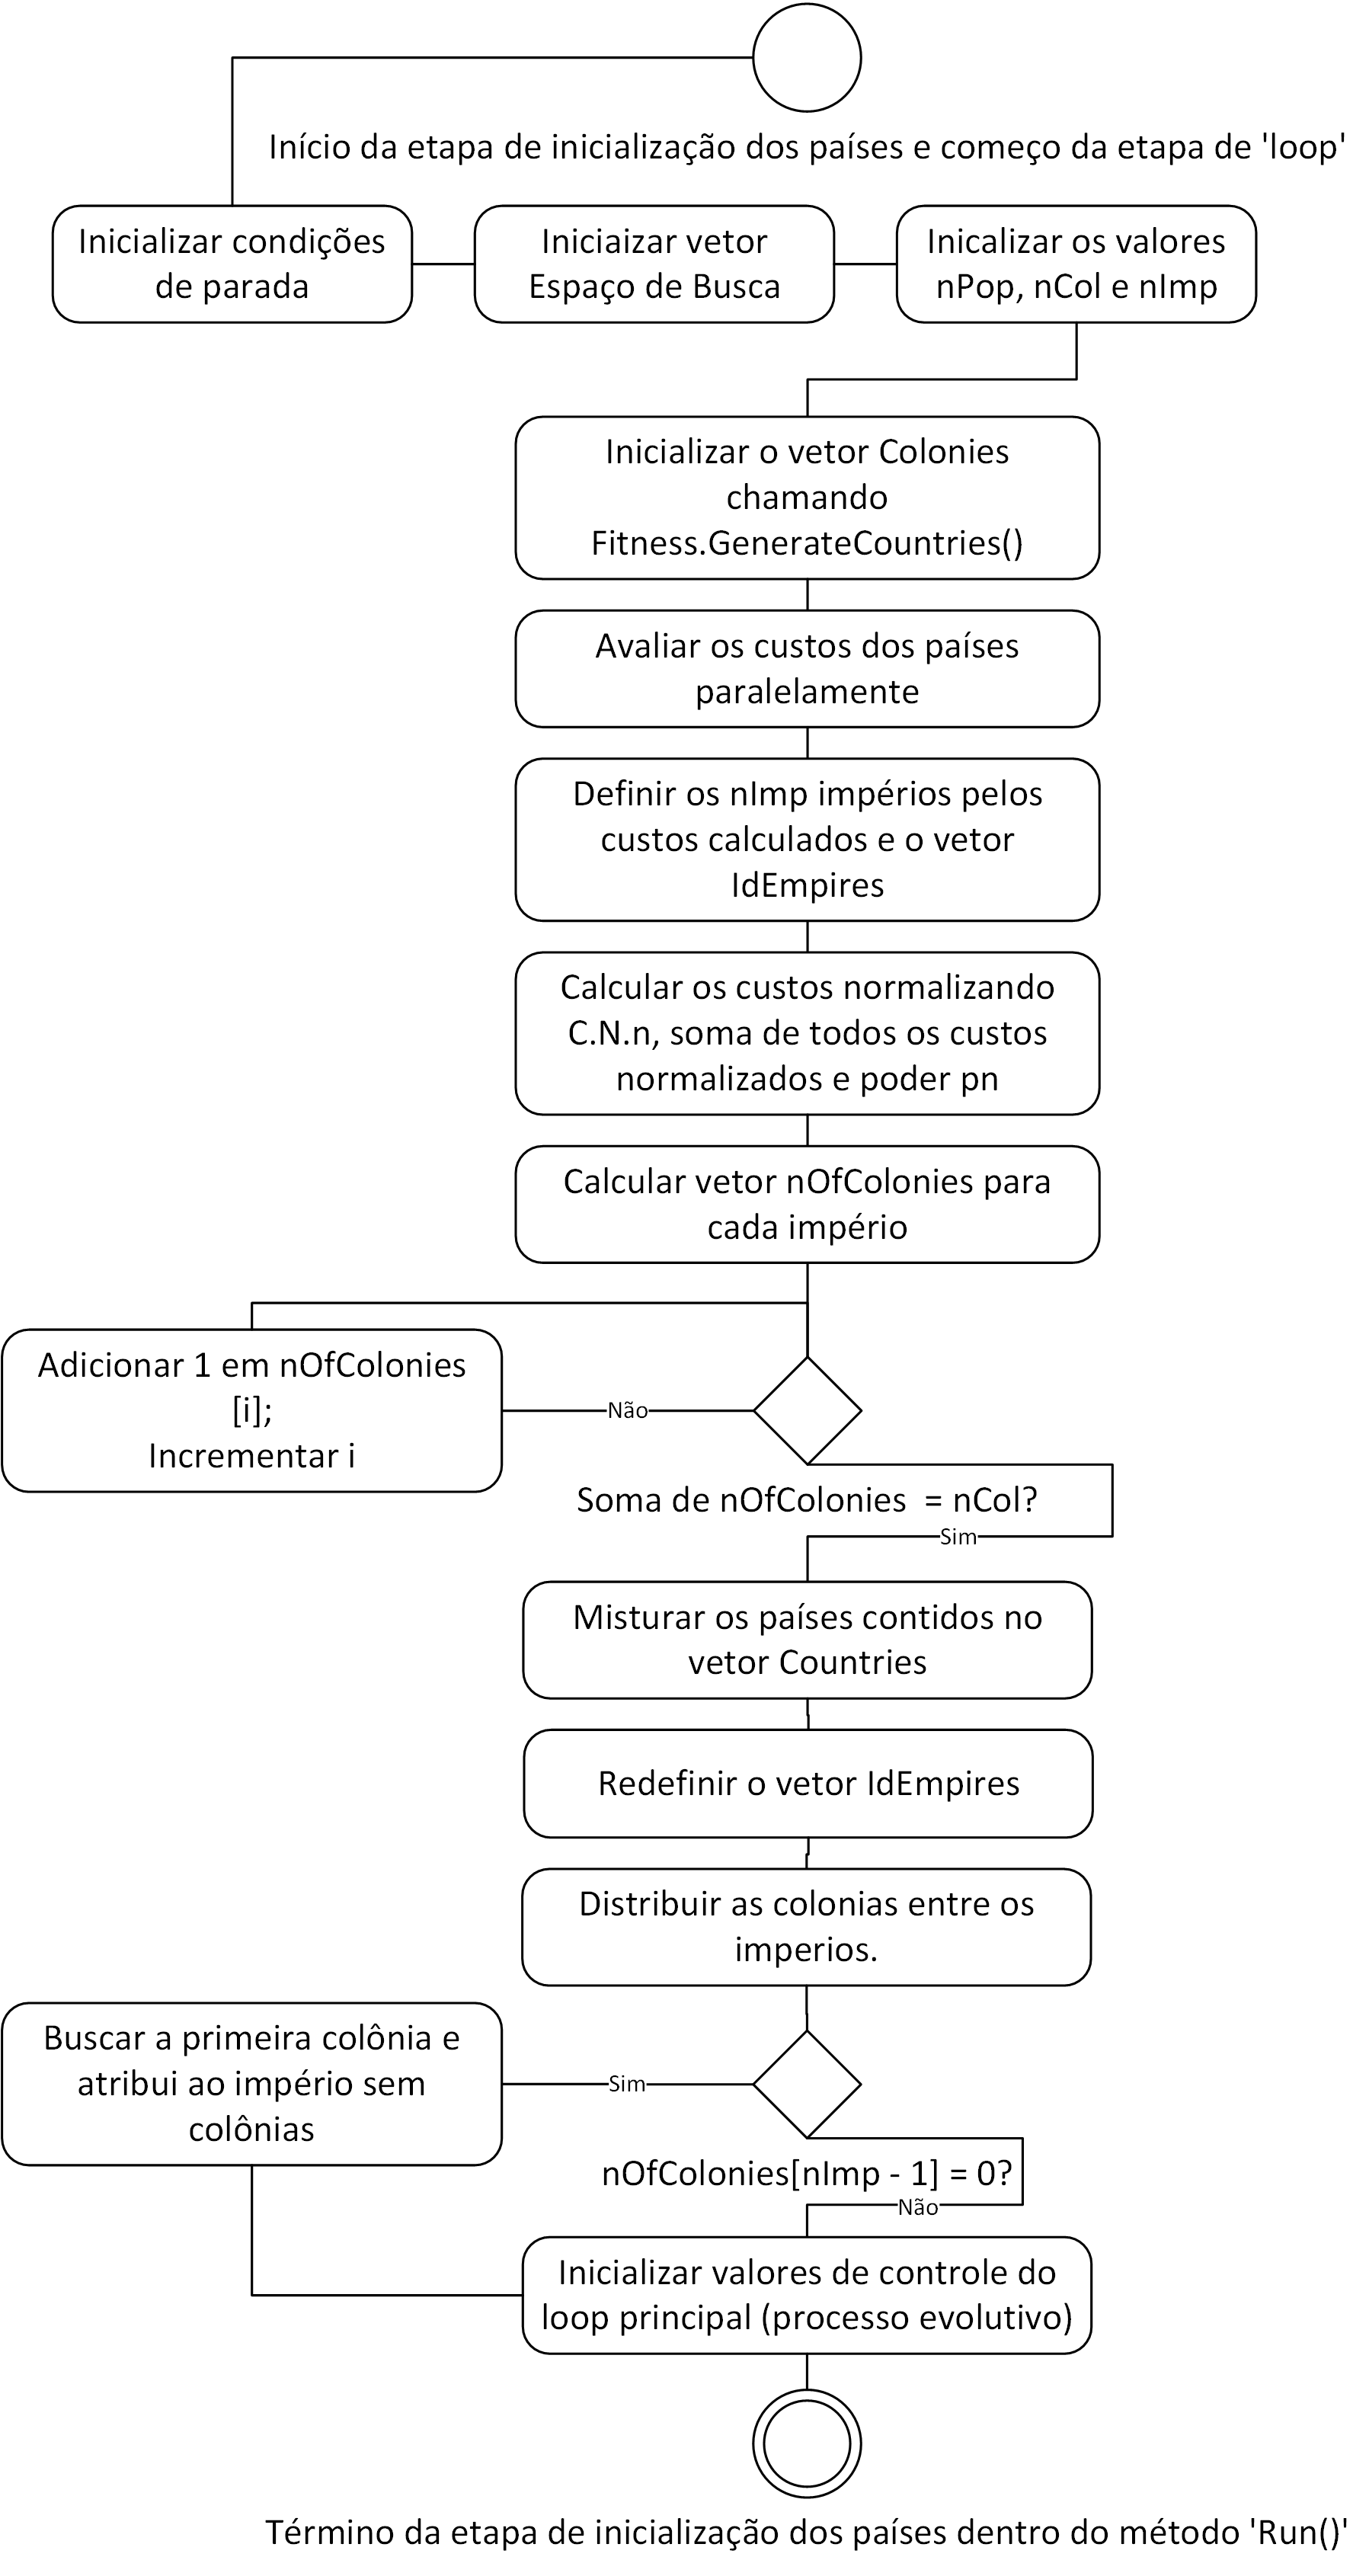
\includegraphics[scale=0.7]{Figuras/Fluxograms-RunMethodStart.png}
	\caption{Fluxograma da etapa de inicialização no método Run}
	\label{fig:Fluxograms-RunMethodStart}
	\end{figure}
    
Antes que se distribua as colônias para os impérios, o vetor contendo os países deve ser misturado, pois as colônias devem ser aleatoriamente distribuídas entre os impérios. Quando se efetua esta mistura, o vetor \emph{IdEmpires} deve ser redefinido para que se atualize os novos índices dos países imperialistas, pois o vetor de países \emph{Countries} sempre conterá os países imperialistas e suas colônias, e também nunca terá sua quantidade alterada. O ICA é um algoritmo que não destrói ou constrói países durante seu processo evolutivo, ele apenas altera seus atributos. 

A distribuição das colônias para os impérios ocorre iterando-se em \emph{i} inicialmente pelo vetor de impérios \emph{IdEmpire} uma única vez, e a cada iteração de \emph{i}, itera-se em \emph{j}, \emph{nOfColonies[i]}, efetuando assim a relação império (pelo vetor \emph{IdEmpire}) por número de colônias (pelo vetor \emph{nOfColonies}). Agora basta ir iterando o valor \emph{nCountry} sempre que se atribuir uma colônia a um império. Esta atividade que distribui as colônias entre os impérios pode ser melhor visualizada pelo fluxograma apresentado na Figura \ref{fig:Fluxograms-RunMethodEmpireDistribution}.

 \begin{figure}[h]
	\centering	
	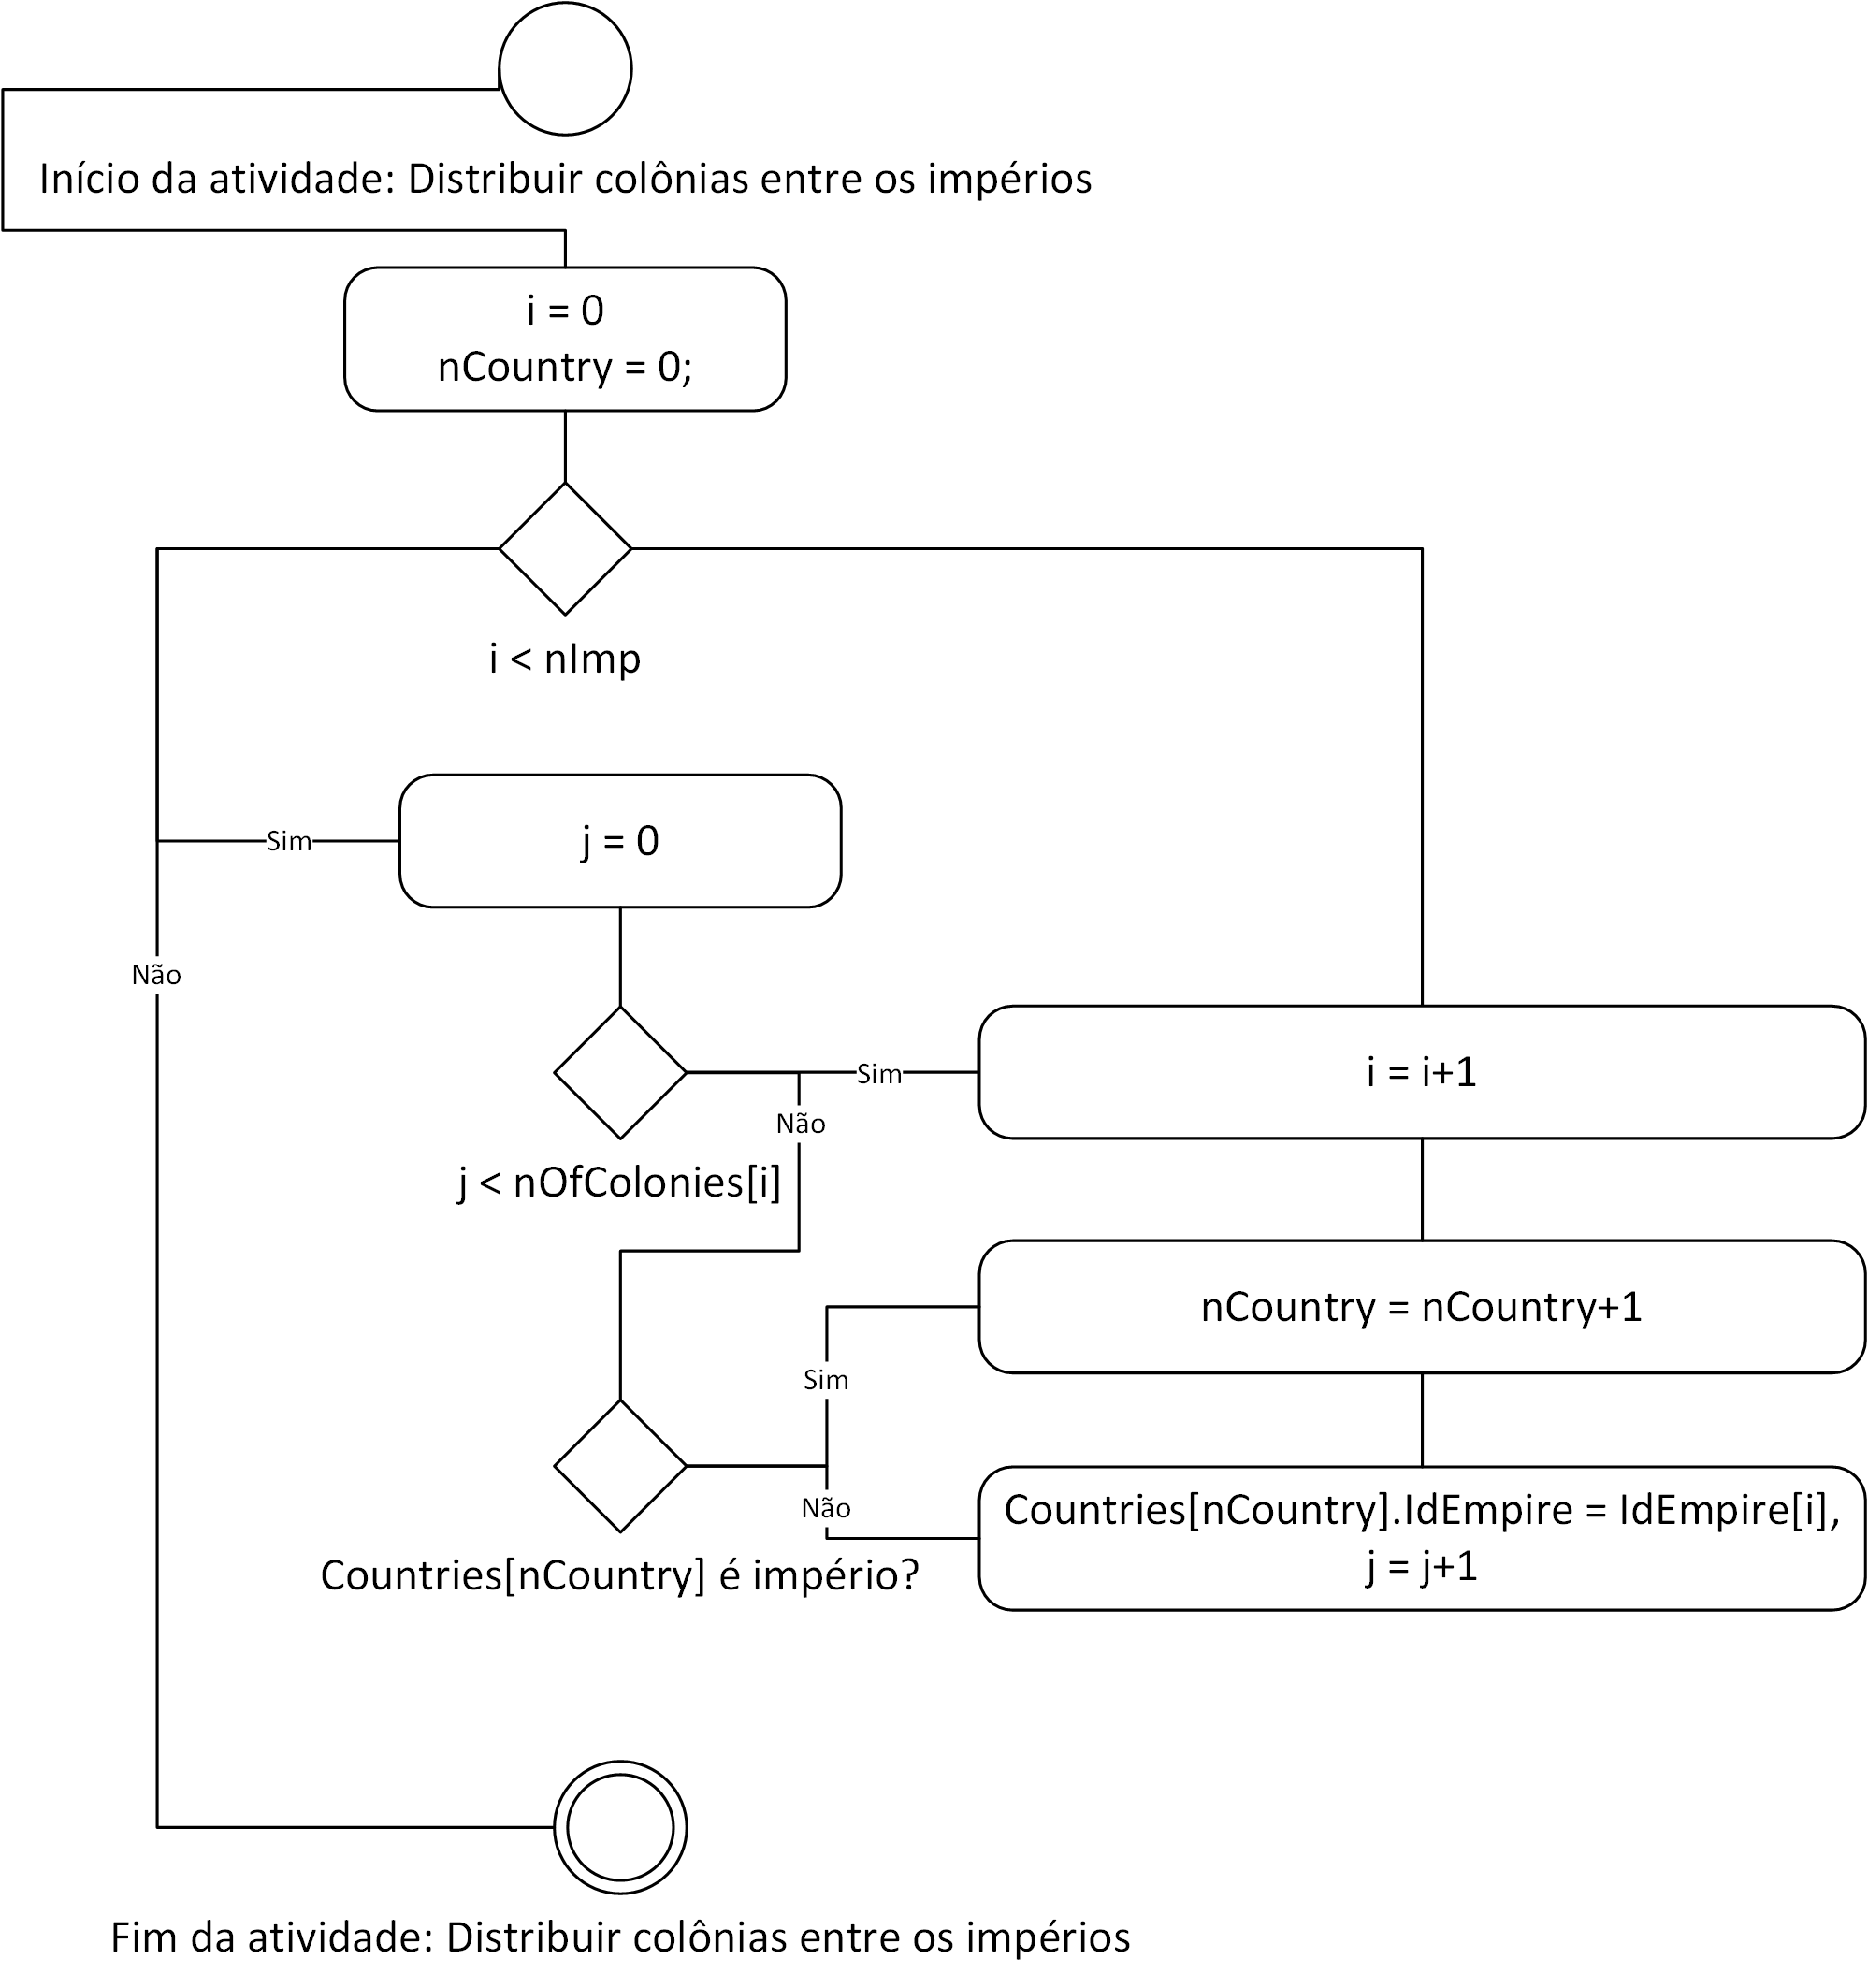
\includegraphics[scale=0.7]{Figuras/Fluxograms-RunMethodEmpireDistribution.png}
	\caption{Fluxograma sobre a distribuição de colônias entre os impérios}
	\label{fig:Fluxograms-RunMethodEmpireDistribution}
	\end{figure}

Após a distribuição das colônias entre os impérios, ocorre uma verificação para certificar-se de que o último império tem pelo menos uma colônia, e caso ele não tenha, a ele é atribuída uma colônia arbitrária de um dos outros império. Note que esta etapa traz a impressão de ser semelhante a etapa que verifica se a soma do vetor \emph{nOfColonies} é igual a \emph{nCol}, porém são coisas distintas, pois a condição \emph{nOfColonies} == \emph{nCol} não implica que todos os impérios devam ter pelo menos 1 colônia. 

Com a etapa de inicialização dos países finalizada, agora existem impérios, os quais possuem colônias que foram atribuídas de forma proporcional e arbitrariamente, e estes impérios e suas colônias estão espalhados por todo espaço de busca aleatoriamente, prontos para iniciar o processo evolutivo do ICA. O processo evolutivo no ICA caracteriza-se por um processo iterativo (\emph{loop}) onde os elementos, que já estão dispostos no espaço de busca, começam a alterar seus atributos para encontrar a melhor solução presente neste espaço de busca. Então, durante o processo evolutivo ocorrem várias operações nas colônias  e impérios de forma a atingir a melhor solução, e consequentemente parar este processo iterativo. 

Observando novamente o fluxograma do ICA apresentado na metodologia pela figura \ref{fig:Fluxograms-ICACanonic}, é possível notar as operações:
\begin{itemize}
\item Assimilação colonial - movimentação da colônia para o império,
\item Possessão imperial - colônia mais poderosa toma o império para si, e
\item Competição imperialista - a colônia mais fraca do império mais fraco é passada para o império mais propenso a tê-la.
\end{itemize}

A delimitação destes elementos pode ser observada na Figura\ref{fig:Fluxograms-ICACanocicDetailed}, assim como a separação entre a etapa de inicialização e o processo evolutivo. Estas operações são suficientes para encontrar soluções em qualquer espaço de busca, porém, este trabalho apresenta algumas adições de operações  ou melhoras de alguns métodos, a fim de otimizar tanto o tempo de convergência quanto a precisão da busca pela melhor solução, e ainda, de modo que estas operações ocorram de forma agregada ao fluxo anterior. Estas alterações são mencionadas nas subseções seguintes, e aqui nesta seção serão apresentados apenas alguns detalhes referentes ao funcionamento de tais alterações. 

	A primeira etapa, logo após a entrada no \emph{loop} principal é a de notificação, que envia para todos os elementos registrados nesta classe uma cópia do vetor de países \emph{Countries} e o valor da década atual \emph{CurrentDecade}. Assim, qualquer um que esteja ouvindo pode fazer o rastreio de todos os países e impérios durante as décadas.

 \begin{figure}[h]
	\centering	
	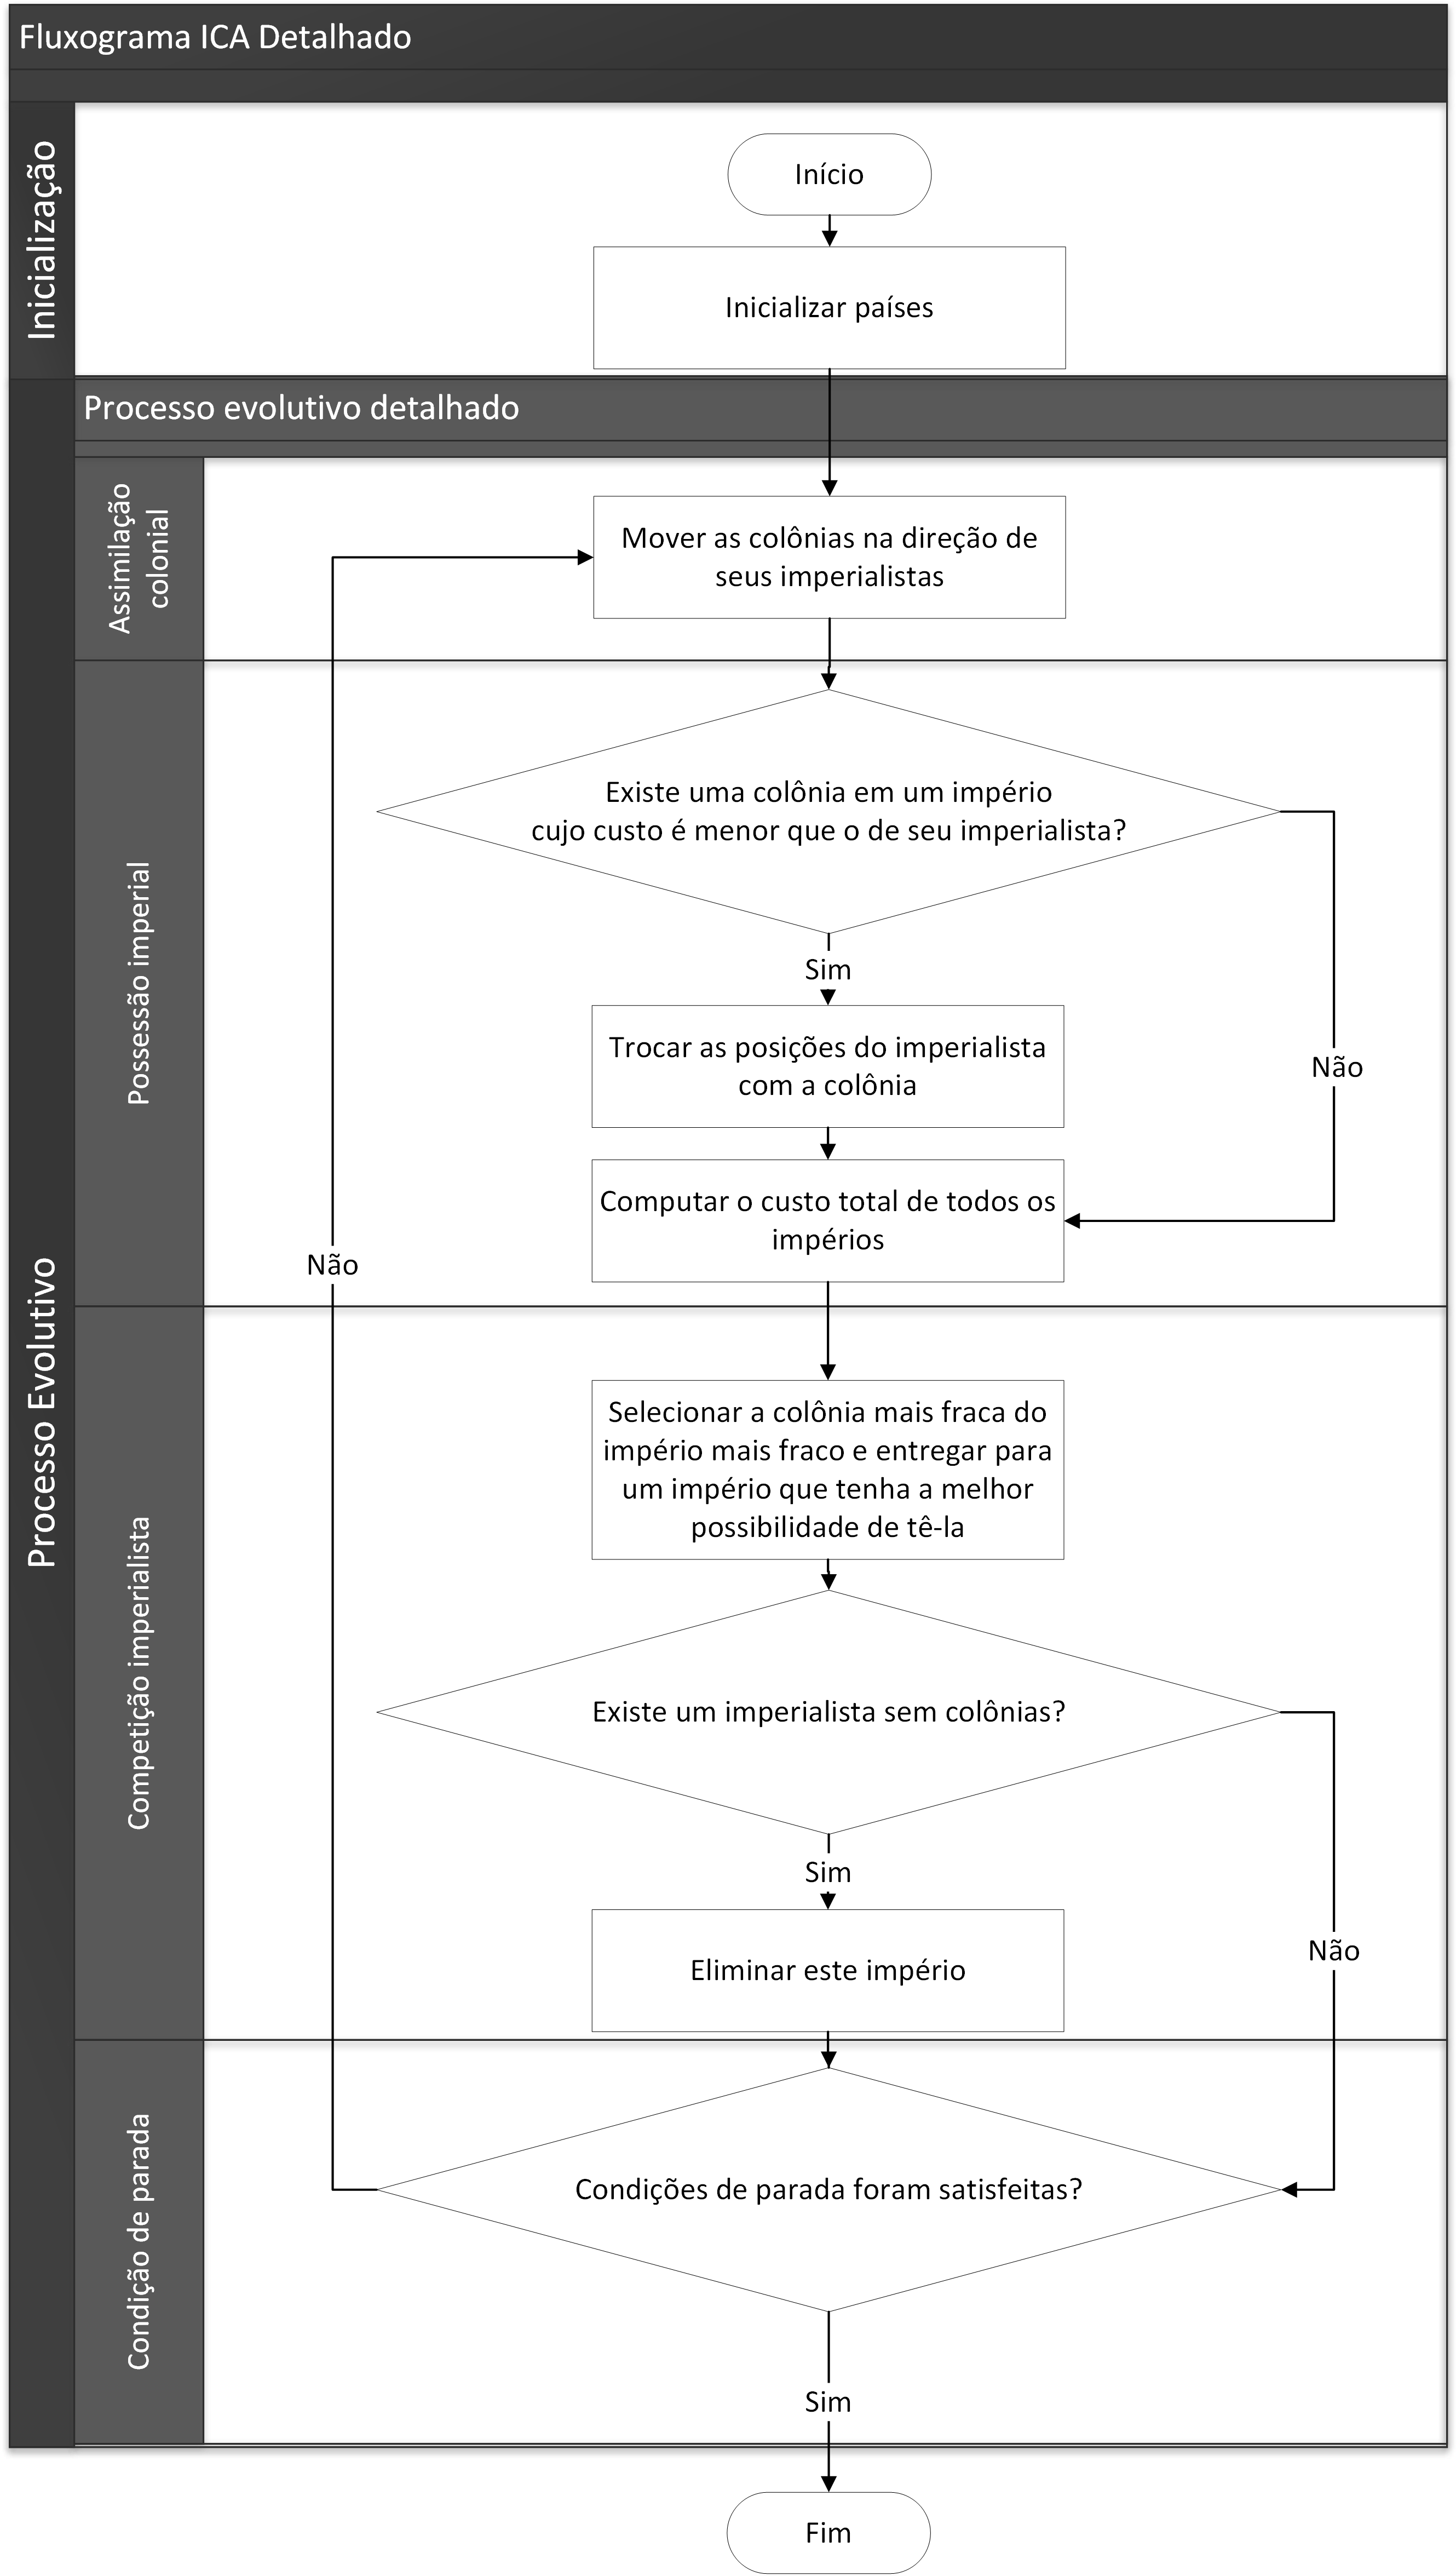
\includegraphics[scale=0.5]{Figuras/Fluxograms-ICACanocicDetailed.png}
	\caption{Fluxograma ICA detalhado}
	\label{fig:Fluxograms-ICACanocicDetailed}
	\end{figure}
	
Foram efetuadas algumas alterações na ordem de algumas etapas, mas sem alterar o funcionamento do ICA. Assim, para esta próxima etapa foi inserido o bloco responsável por fazer a verificação das condições de parada, que antes de fazer uma verificação pela lista que contém todas estas condições de parada, passa por uma pré verificação, que não é uma condição de parada, que verifica se o ICA deve convergir para apenas um império (se o número de impérios é 1). Tal lógica de entrada para verificação das condições de parada pode ser vista no diagrama da Figura \ref{fig:Fluxograms-StopConditions}.

 \begin{figure}[h]
	\centering	
	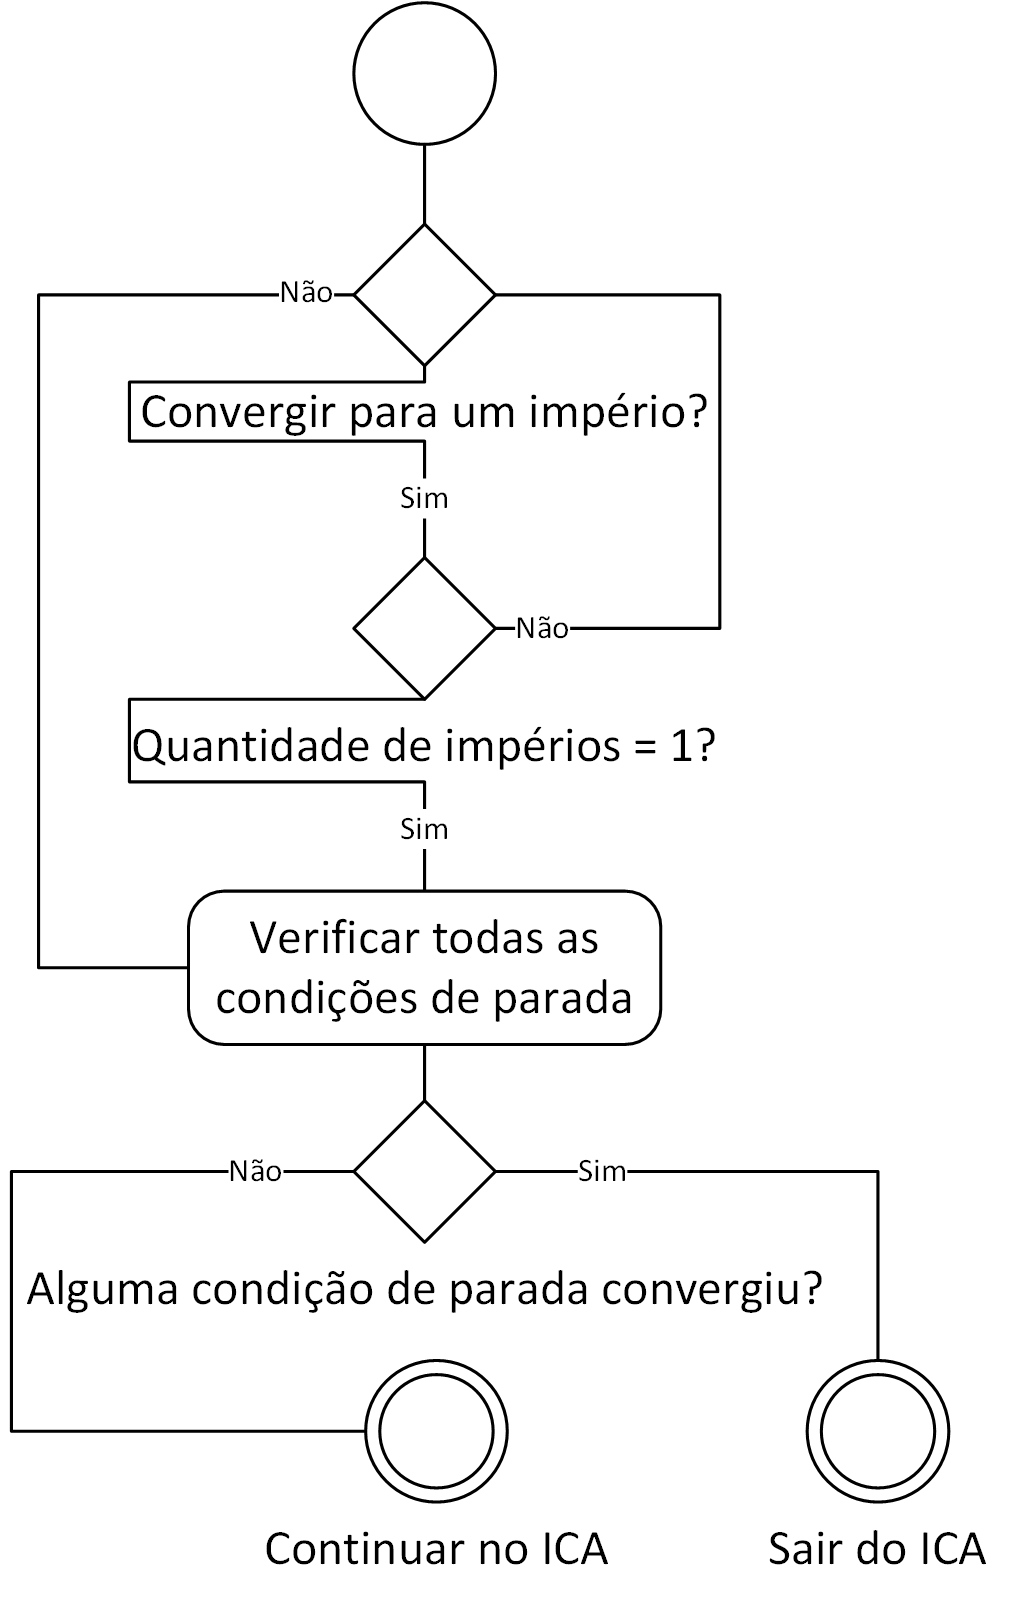
\includegraphics[scale=0.7]{Figuras/Fluxograms-StopConditions.png}
	\caption{Fluxograma sobre as condições de parada}
	\label{fig:Fluxograms-StopConditions}
	\end{figure}

Logo após a verificação das condições de parada, atualiza-se o valor da taxa de revolução (Revolução é uma nova operação adicionada, semelhante a operação de mutação do GA canônico e será descrita em um tópico separado), e em seguida efetua uma iteração por todos os impérios, fazendo a chamada para duas operações, sendo a primeira, a operação de assimilação colonial, que move as colônias em direção ao seu país imperialista, e a segunda, a nova operação de revolução, que por sua vez gera novos valores completamente aleatórios para o vetor de atributos de um dado país baseando-se em uma chance de ocorrência relativa a taxa de revolução mencionada anteriormente. Ambas operações são implementadas em métodos que recebem como parâmetro o valor do índice do império no vetor de colônias e uma lista de países contendo apenas as colônias pertencentes a este império.

Assim que a chamada destas duas operações ocorrer para todos os impérios, sabe-se que todas as colônias efetuaram a movimentação em direção ao seu imperialista e que uma porcentagem destas colônias pode ter passado pelo processo de revolução. Como os atributos destes países são alterados, é essencial que se recalcule os custos de todos os países, atualizando-os para que sejam utilizados nas demais operações do ICA. Nota-se também que apenas estas duas operações são as responsáveis por alterar os atributos dos países, assim, além de essencial, é imprescindível que a atualização dos custos ocorra.

O cálculo dos custos é feito pela chamada do método Eval pertencente ao objeto \emph{Fitness}, que por sua vez é o responsável por avaliar um dado país segundo o problema modelado pelo objeto em questão que implementa os métodos da interface \emph{IFitness}. A avaliação dos países é efetuada de modo paralelo não obstrutivo, ou seja, a avaliação de um dado país não depende dos demais países (Observa-se que a não obstrução no escopo do ICA é garantida, porém quando se implementa a interface \emph{IFitness} deve-se tomar cuidado para que o compartilhamento de recursos entre as tarefas não faça com que o processamento da avaliação de um país seja interrompido pelo processamento de outra avaliação, que requer o uso do mesmo recurso compartilhado). O fluxo do ICA só é continuado quando a avaliação de todos os países é finalizada, independente de se estar avaliando em paralelo ou em série.

Seguindo o fluxo, a próxima operação verifica se existe uma colônia com poder maior que seu império, e caso positivo, esta colônia se torna o país imperialista, tomando para si as colônias do antigo império. São feitas diversas chamadas a esta operação, de forma iterativa, passando por todos os impérios, para que tal verificação possa ser efetuada através de um método que recebe como parâmetro o valor do índice do império no vetor de países \emph{Countries} e a referência do vetor que contém os índices de todos os impérios \emph{IdEmpires}.  


Esta operação executa, inicialmente, uma seleção no vetor \emph{Countries} a fim de filtrar todas as colônias do império em questão, em seguida, é necessário que verifique-se se esta seleção resultou em um número de colônias igual a 0, o significa que este é um país imperialista sem colônias, e caso isto ocorra, para manter a consistência do ICA para as próximas operações, deve-se eliminar este império. Como mencionado anteriormente, um império quando é eliminado, têm seu país imperialista se tornando uma colônia do império mais forte, assim, esta operação segue os seguintes passos durante sua execução:
\begin{itemize}
\item Buscar pelo índice do melhor império e armazena localmente em \emph{bestEmpireId}.
\item Transforma o país imperialista sem colônias em uma colônia do país de índice \emph{bestEmpireId}.
\item Remove o índice do país imperialista que se tornara colônia, do vetor de índices de impérios \emph{IdEmpires} (sendo este o primeiro motivo de se passar a referência do vetor \emph{IdEmpires}, pois ele será atualizado). 
\end{itemize}

Caso a seleção das colônias seja maior que 0, significa que pode existir uma colônia cujo poder é maior que o de seu império, então se esta verificação for verdadeira, a colônia possuirá seu império, transformando o antigo país imperialista e suas colônias em colônias suas. Para efetuar esta troca executa-se a operação na sequencia:

\begin{itemize}
\item Armazenam-se ambos os índices, da colônia que tomara o império e do país imperialista respectivamente em \emph{newEmpireId} e \emph{oldEmpireId},  em cache local;
\item Transforma o país de índice \emph{newEmpireId} o novo país imperialista.
\item Transforma o país de índice \emph{oldEmpireId} em uma colônia do país de índice \emph{newEmpireId}.
\item Passa pela lista de colônias do antigo império alterando o índice das colônias para \emph{oldEmpireId}, obviamente com exceção do país de índice \emph{newEmpireId}, que agora é o novo país imperialista.   
\item Altera o valor do \emph{IdEmpires}, atualizado-o com o valor do índice do novo império \emph{newEmpireId} (sendo este o segundo motivo para se passar a referência do vetor \emph{IdEmpires} para este método).
\end{itemize}

Assim termina-se a etapa de possessão imperial, que pode efetuar duas operações no vetor \emph{IdEmpires}, sendo estas, o rebaixamento de um império sem colônias para colônia do império mais poderoso e a própria possessão imperial propriamente dita. Nota-se que a primeira deve sempre ocorrer antes de operações que fazem o remanejamento de colônias e impérios, assim, operações descritas mais adiante, que fazem tal remanejamento, já implicará nesta pré verificação.

A próxima operação, idealizada por \cite{roche2011imperialist}, é uma das adições ao fluxo normal do ICA e diz respeito a união de dois impérios próximos. Esta funcionalidade agiliza o processo de convergência, pois quando dois impérios se aproximam e ambos possuem muitas colônias, seriam necessárias diversas décadas até que o império mais forte conseguisse assimilar por completo o império mais fraco, utilizando-se apenas a competição imperialista, tomando colônia por colônia.

Esta operação calcula um valor de limiar para união de dois impérios, sendo que este valor é definido com o valor armazenado em \emph{UnitingThreshold} vezes a norma do do vetor que contém os valores dos tamanhos do espaço de busca de cada dimensão, representado por \emph{SpaceSearchSize}, então tem-se que 

\[Limiar = UnitingThreshold \cdot Norma2(SpaceSearchSize) \]

Com o limiar já calculado, itera-se por cada império comparando-o com os demais impérios. Para comparar um império com outro, e de fato iniciar o processo de união, deve-se antes calcular a distância entre ambos, e se esta distância for menor que o limiar definido acima, une-se os dois impérios. Assim, a operação de união entre impérios é muito semelhante com a operação de eliminação de um império, apenas adicionando a transferência das colônias do império mais fraco para o mais forte. Nota-se que este método exige a referência do vetor \emph{IdEmpires} para que ele possa ser alterado também no escopo (global) em que este método fora chamado.

Por fim, o último método a ser chamado é o responsável por executar a competição imperialista, removendo a pior colônia do pior império e dando esta colônia para o império mais propenso a possuí-la. Nota-se novamente que este método também exige a referência do vetor \emph{IdEmpires} para que ele possa ser alterado também no escopo em que este método foi chamado, pois assim que uma tomada de colônia ocorrer, pode acontecer de um império ficar sem colônias, então a eliminação deste império ocorrerá logo após a tomada (ou tentativa de tomada) de uma colônia deste império.

Os detalhes do que ocorre dentro deste método podem ser vistos no fluxograma da Imagem \ref{fig:Fluxograms-RunMethodImperialistCompetition}. Observe que antes mesmo de se iniciar o processo, existem duas verificações sendo a primeira a verificação da chance de ocorrência da competição nesta década, e a segunda é a verificação de certificação por número de impérios (obviamente é necessário que existam no mínimo 2 impérios para que se ocorra a competição imperialista). Logo após as verificações calcula-se o poder total de todos os impérios baseando-se no seu custo e em uma proporção da média dos custos de suas colônias, como pode-se ver no trecho abaixo.

\[
possessionProbability[i] = \frac{power[i]}{ \sum(power)}, i : 0 \space até\space nImp
\]

Com o poder total de cada império calculado e armazenado no vetor \emph{power} seleciona-se qual é o império mais fraco, e em seguida normaliza-se os custos totais, sobrescrevendo os valores do vetor \emph{power}, e calcula-se o vetor de probabilidade de possessão \emph{possessionProbability}.

A partir do vetor de probabilidade de possessões seleciona-se o império que mais tiver a probabilidade de possuir uma colônia do império mais fraco selecionado anteriormente. Na conceituação do ICA seleciona-se a colônia mais fraca do império mais fraco, mas nesta implementação optou-se por selecionar uma colônia aleatória do império mais fraco com a intenção de acelerar a convergência. Lembrando que a seleção da colônia só acontecerá se o número de colônias do império for maior ou igual a 1. Por fim, verifica se o império que teve a colônia trocada não tem mais colônias, e caso verdadeiro elimina-se este império fazendo com que ele se torne uma colônia do império mais forte.
    
 \begin{figure}[h]
	\centering	
	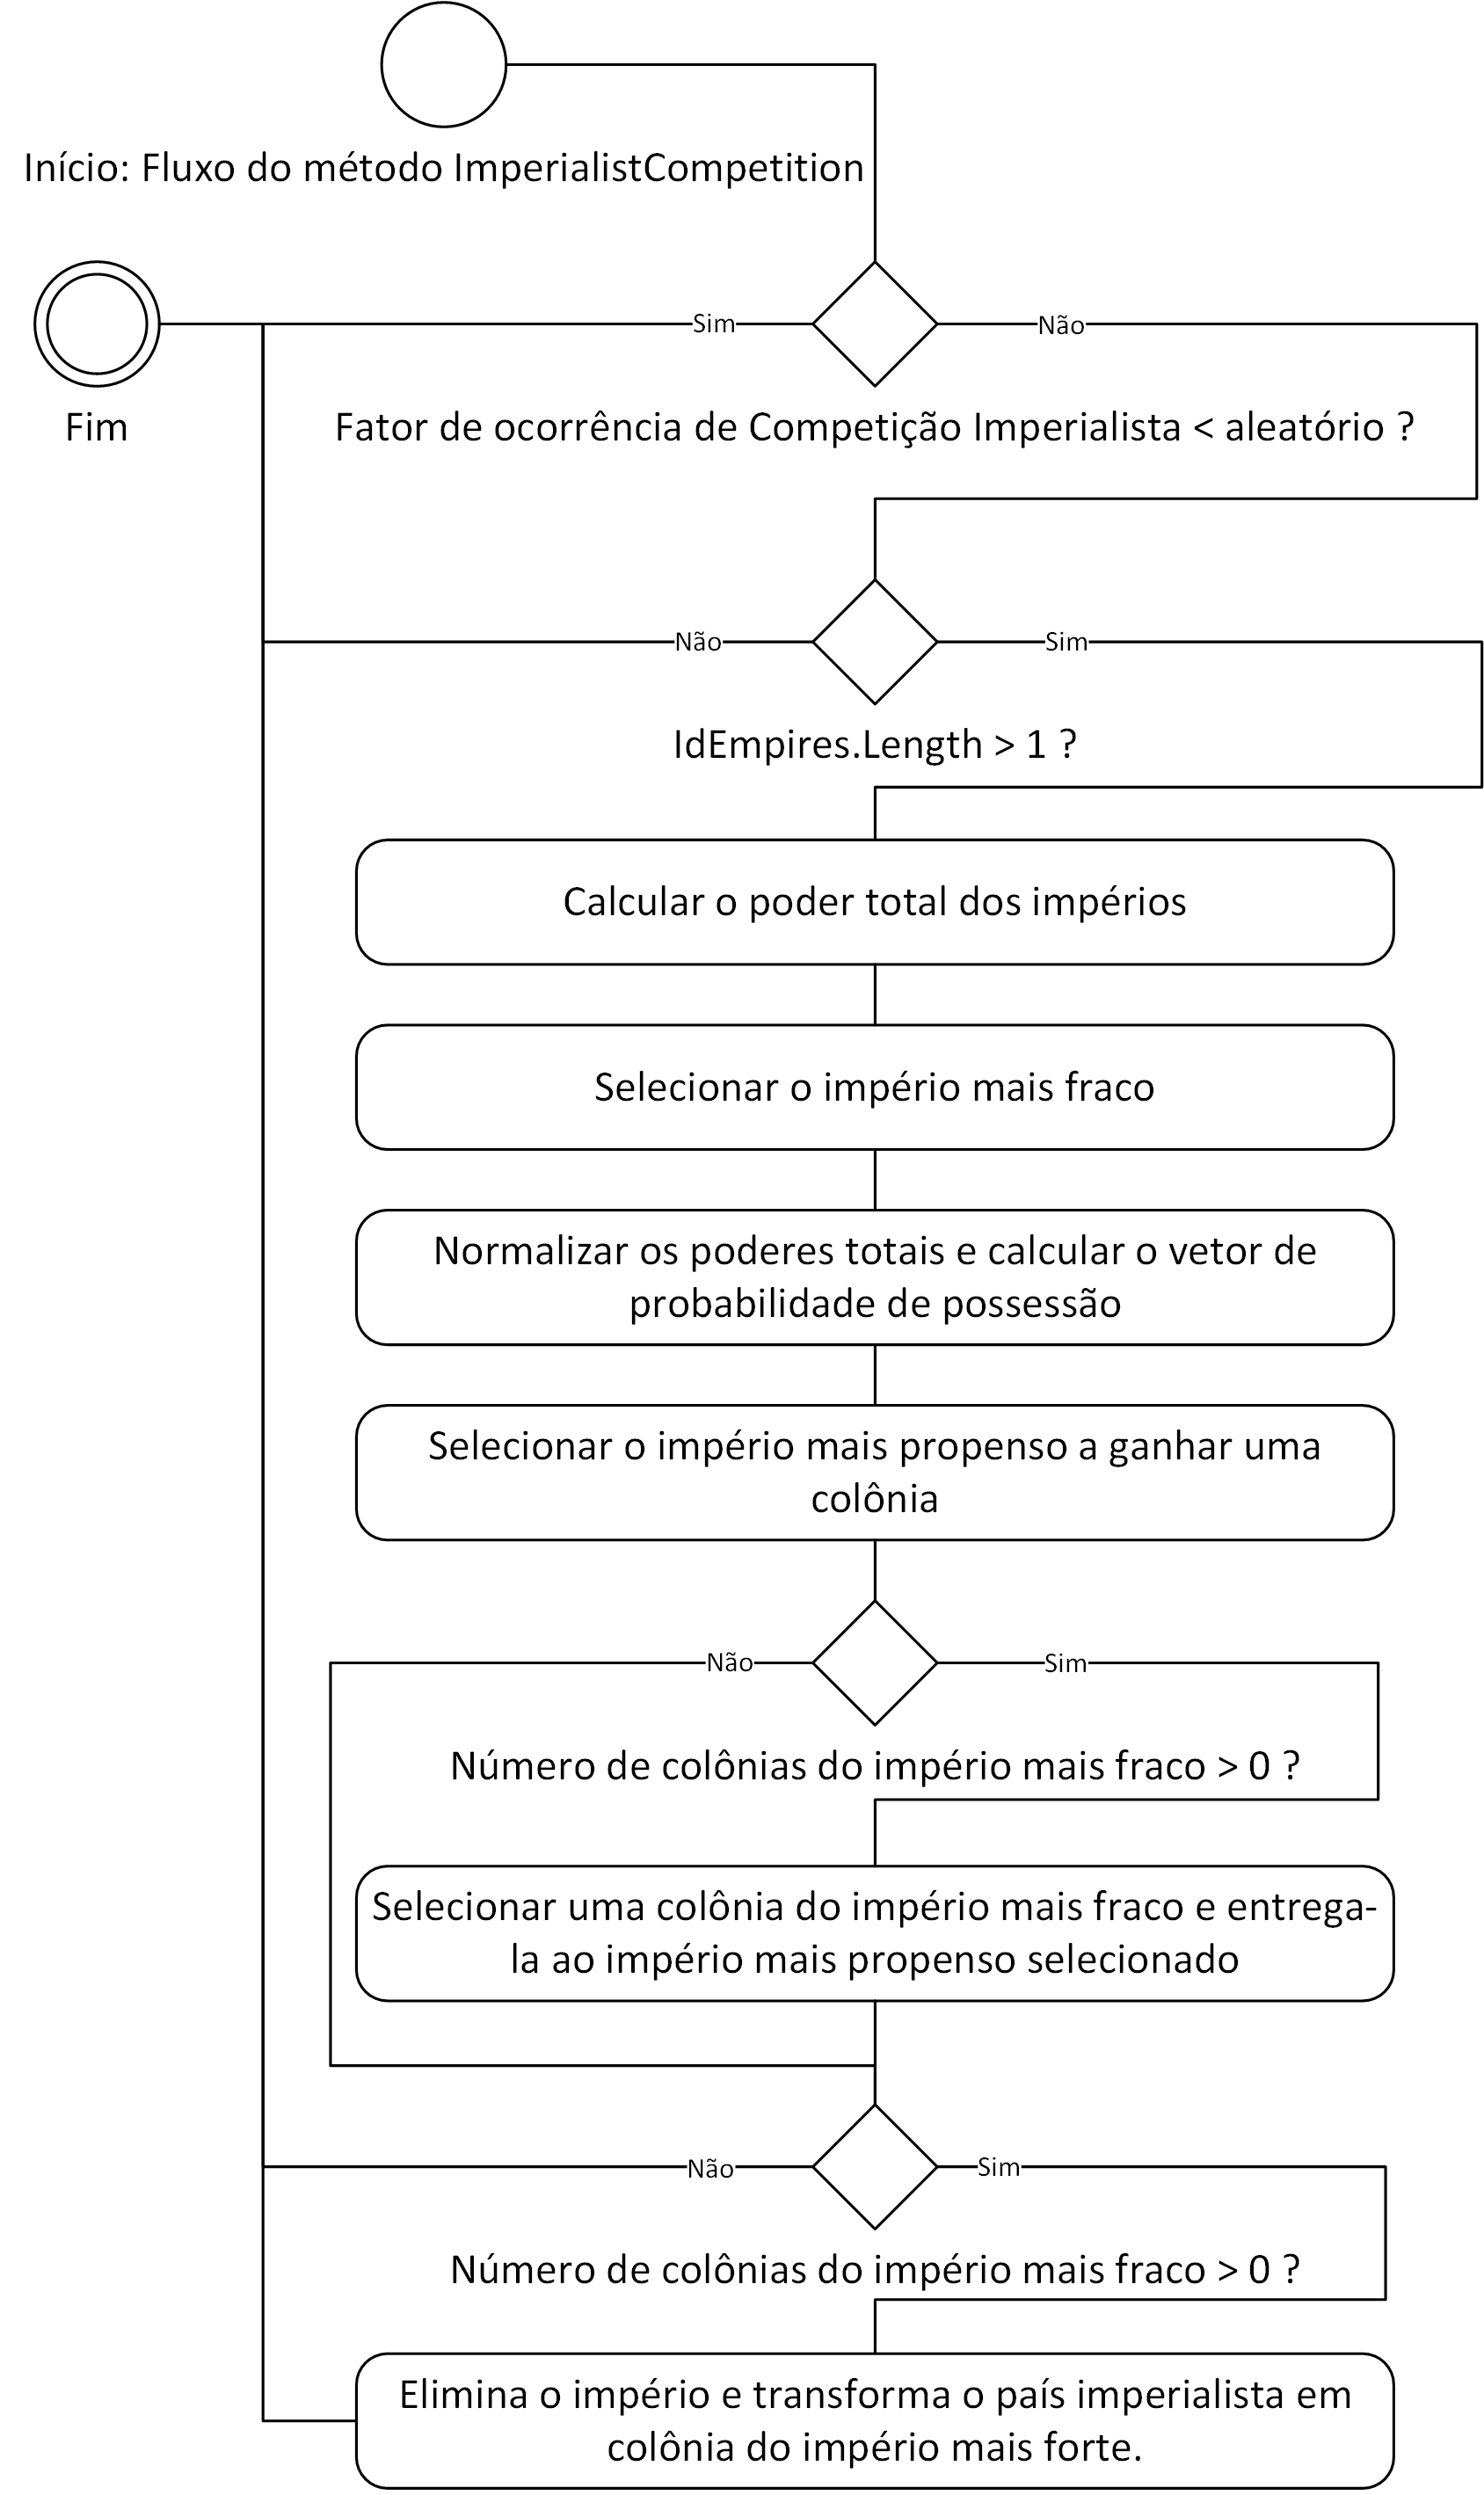
\includegraphics[scale=0.7]{Figuras/Fluxograms-RunMethodImperialistCompetition.png}
	\caption{Fluxograma competição imperialista}
	\label{fig:Fluxograms-RunMethodImperialistCompetition}
	\end{figure}
    
Após terminar a chamada do método \emph{ImperialistCompetition}, conclui-se o \emph{loop} principal incrementando o valor de década. Ao retornar  para o início do \emph{loop}, são verificadas as condições de parada até que alguma delas retorne o valor de parada e o algoritmo finaliza sua execução. Quando o algoritmo termina a execução do método \emph{Run}, a lista de colônias estará posicionada no lugar ótimo para o problema em questão (isto é, seus atributos já estarão otimizados). Os dados podem ser acessados através de suas propriedades públicas pertencentes ao objeto do tipo \emph{ImperialistCompetition} instanciado em memória.

O desenvolvimento do ICA orientado a objetos proporciona principalmente praticidade no que diz respeito a modelagem genérica de problemas, ou seja, qualquer problema que se queira otimizar pode fácil e rapidamente ser implementado para que o ICA consuma os métodos da interface \emph{IFitness} que descreve o problema a ser otimizado. Outra vantagem que a orientação a objetos trouxe foi a organização dos conceitos, de forma que se possa ter um profundo entendimento de como o algoritmo efetua suas operações até que se chegue em soluções ótimas. E por fim, num contexto geral a modelagem do ICA foi pensada para que ele demonstrasse desempenho ótimo, dependendo basicamente do tempo que a função de avaliação leva para executar e nada mais.

Todas estas alterações de otimização do ICA apenas foram possíveis através do desenvolvimento Orientado a Objetos, que permite encapsular as entidades e desenvolver suas lógicas separadas em métodos bem definidos, assim, abstrai-se a solução em objetos capazes de atender e concentrar os aspectos essenciais do contexto (competição imperialista) de uma forma bem definida. Assim, a implementação do ICA permite fácil adaptação a qualquer abordagem ou ambientação de otimização para um dado problema.







\subsection{Exemplos de aplicação do ICA genérico}

Abaixo apresentam-se dois cenários distintos de implementação do ICA Generalista abordando dois problemas, G1 e G2. O primeiro é uma implementação mais simples, em que a avaliação se dá pela necessidade de minimização da função matemática:

\begin{equation}
\centering
\begin{split}
\text{Problema G1:} \\
& F(x,y) = x \cdot \sin(4 \cdot x)+ 1.1 \cdot y \cdot \sin(2 \cdot y), \\ 
& 0 < x,y < 10, \\ 
& mínimo: f(9.039, 8.6680) = -18.5547.
\end{split}
\end{equation}

A implementação deste problema fica muito simples, pois será um problema de minimização de função matemática dentro de um intervalo fechado, assim, o diagrama de classes simplificado fica como apresentado na Figura \ref{fig:Problems-G1Model}.

\begin{figure}[h]
	\centering
	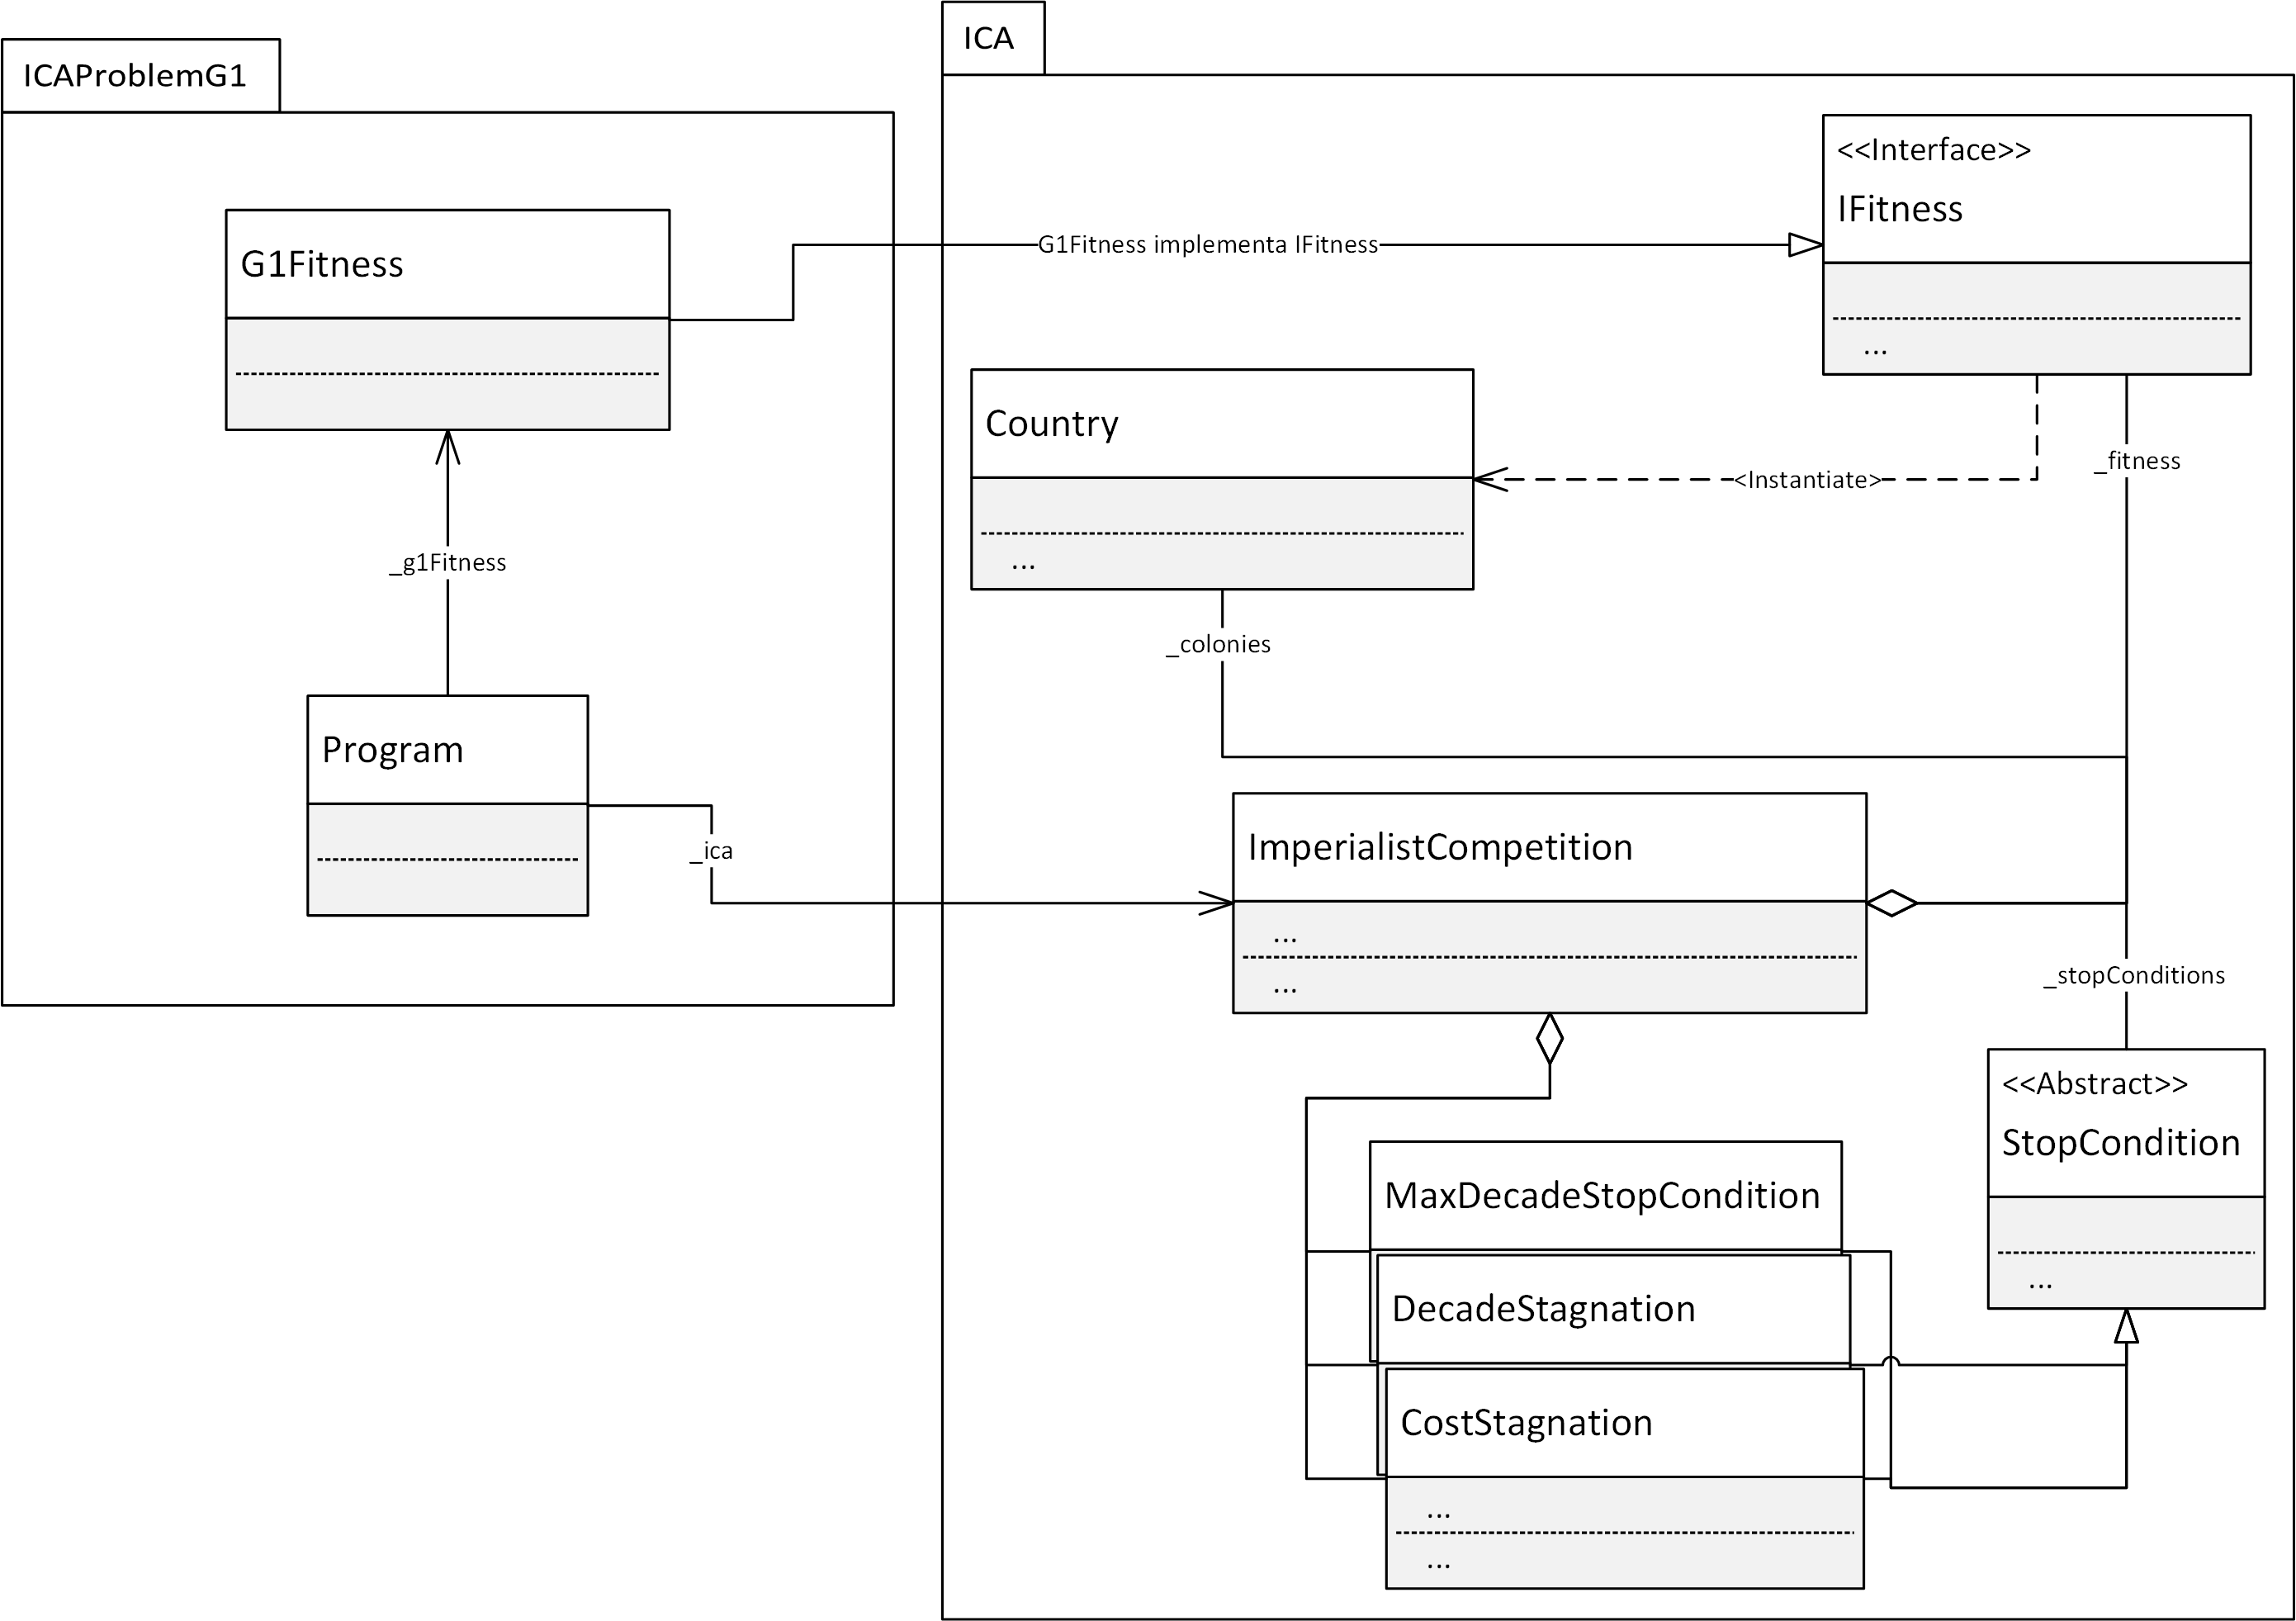
\includegraphics[scale=0.6]{Figuras/Problems-G1Model.png}
	\caption{Diagrama de classes simplificado do problema G1}
	\label{fig:Problems-G1Model}
\end{figure}

No diagrama simplificado é possível observar que a estrutura inicial do ICA não foi alterada. No desenvolvimento da solução foi criada uma classe \emph{G1Fitness} implementando a interface \emph{IFitness}, na qual define o problema implementando os métodos obrigatórios da interface \emph{IFitness}.

A modelagem deste problema para o ICA é simples, pois tem 2 dimensões onde seus limites são fechados entre 0 e 10. Assim, tem-se que o vetor de atributos para cada país será como apresentado na Figura \ref{fig:Problems-G1Vector}.

\begin{figure}[h]
	\centering
	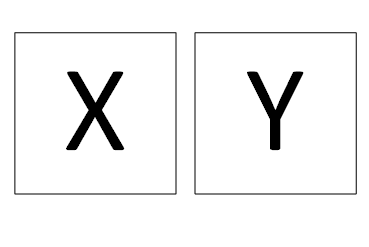
\includegraphics[scale=0.6]{Figuras/Problems-G1Vector.png}
	\caption{Vetor de atributos dos países do problema G1}
	\label{fig:Problems-G1Vector}
\end{figure}

A classe implementada para o problema G1, \emph{G1Fitness}, implementa todos os métodos existentes na interface \emph{IFitness}, sendo assim, a propriedade \emph{Dimensions} apenas retorna o valor 2, pois o problema apresenta duas dimensões(valores de ponto flutuante para \(x\) e para \(y\)). O método \emph{GenerateCountries} não tem nada de especial, apenas cria instâncias simples da classe \emph{Country}, passando os parâmetros necessários no seu construtor padrão, e agrega-as em um vetor para o retorno. E por fim o método \emph{Eval} foi implementado de forma que o custo do país seja o valor da função \(f(x,y)\) tal que \(x = Atributo0\) e \(y = Atributo1\), como descrito no algoritmo \ref{alg:G1Problem}.

\vspace{10px}
\begin{algorithm}[h]
\SetAlgoLined
\KwData{\\ \textbf{ref} element - A referência do país a ser avaliado}
\KwResult{ nenhum valor de retorno, pois altera-se diretamente na referência de element}
x = element.Attributes[0]\;
y = element.Attributes[1]\;
Fxy =\( x \cdot \sin(4.0 \cdot x) + 1.1 \cdot y \cdot \sin(2.0 \cdot y);\)\;
element.Cost = Fxy\;
\caption{ Pseudocódigo método \emph{Eval} do problema G1.}
\label{alg:G1Problem}
\end{algorithm}
\vspace{10px}

Para a apresentação dos resultados foi utilizado o próprio console, e os parâmetros de entrada para o ICA foram: 

Total de países: 128, 

Número de décadas: 512, 

Taxa de revolução: 0.9, 

Taxa de decaimento de revolução: 0.95, 

Coeficiente de assimilação: 0.0001, 

Epsilon: 0.025,

Porcentagem inicial de impérios: 0.15

E no término o melhor indivíduo apresentou os resultados: 

X = 9.0376,

Y = 8.6725,

F(X,Y) = -18.55422.

Este teste apresentou um erro muito menor que 1\%, calculado a seguir: 

\[
e = Abs(Valor Esperado - Valor Obtido ) = Abs((-18.5547) - (-18.55422)) = 0.00048
\]
\[
e\%= 0.00258695\%
\]


O problema G2 exige uma função de avaliação mais complexa, e se dá no seguinte cenário: Dadas duas imagens, sendo que a segunda (I') é a imagem resultado da passagem de um filtro de convolução (M) qualquer sobre a primeira imagem(I), o objetivo do ICA é encontrar qual foi o filtro (máscara de convolução) utilizado neste processamento. O nível de complexidade deste problema é altíssimo, por este ser um problema de inversão de uma função que quando aplicada pode ocasionar em perda ou geração de informação ou ruído no seu resultado, tornando impossível a descoberta do filtro de uma forma direta. A princípio, nos exemplos, foram utilizados apenas filtros de ordem 3 e imagens em escala de cinza(I e I'), todos representados por matrizes de valores.

A implementação do problema G2 foi mais complexa, e usa quase todas as novas funcionalidades do ICA descritas neste trabalho. Na Figura \ref{fig:Problems-G2Model} pode-se observar que não só a classe \emph{IFitness} fora estendida, mas também a classe \emph{Country}. O motivo de se estender a classe \emph{Country} foi para demonstrar duas funcionalidades extras, na qual a primeira tem como objetivo armazenar o resultado obtido pela função de avaliação para que se possa fazer uso posterior sem a necessidade de reprocessamento, já a segunda tem como objetivo alterar o funcionamento da função de randomização de todos os atributos do país, que é chamada sempre que se iniciam os países e também quando ocorre a revolução de uma colônia durante a evolução das décadas. 

\begin{figure}[h]
	\centering
	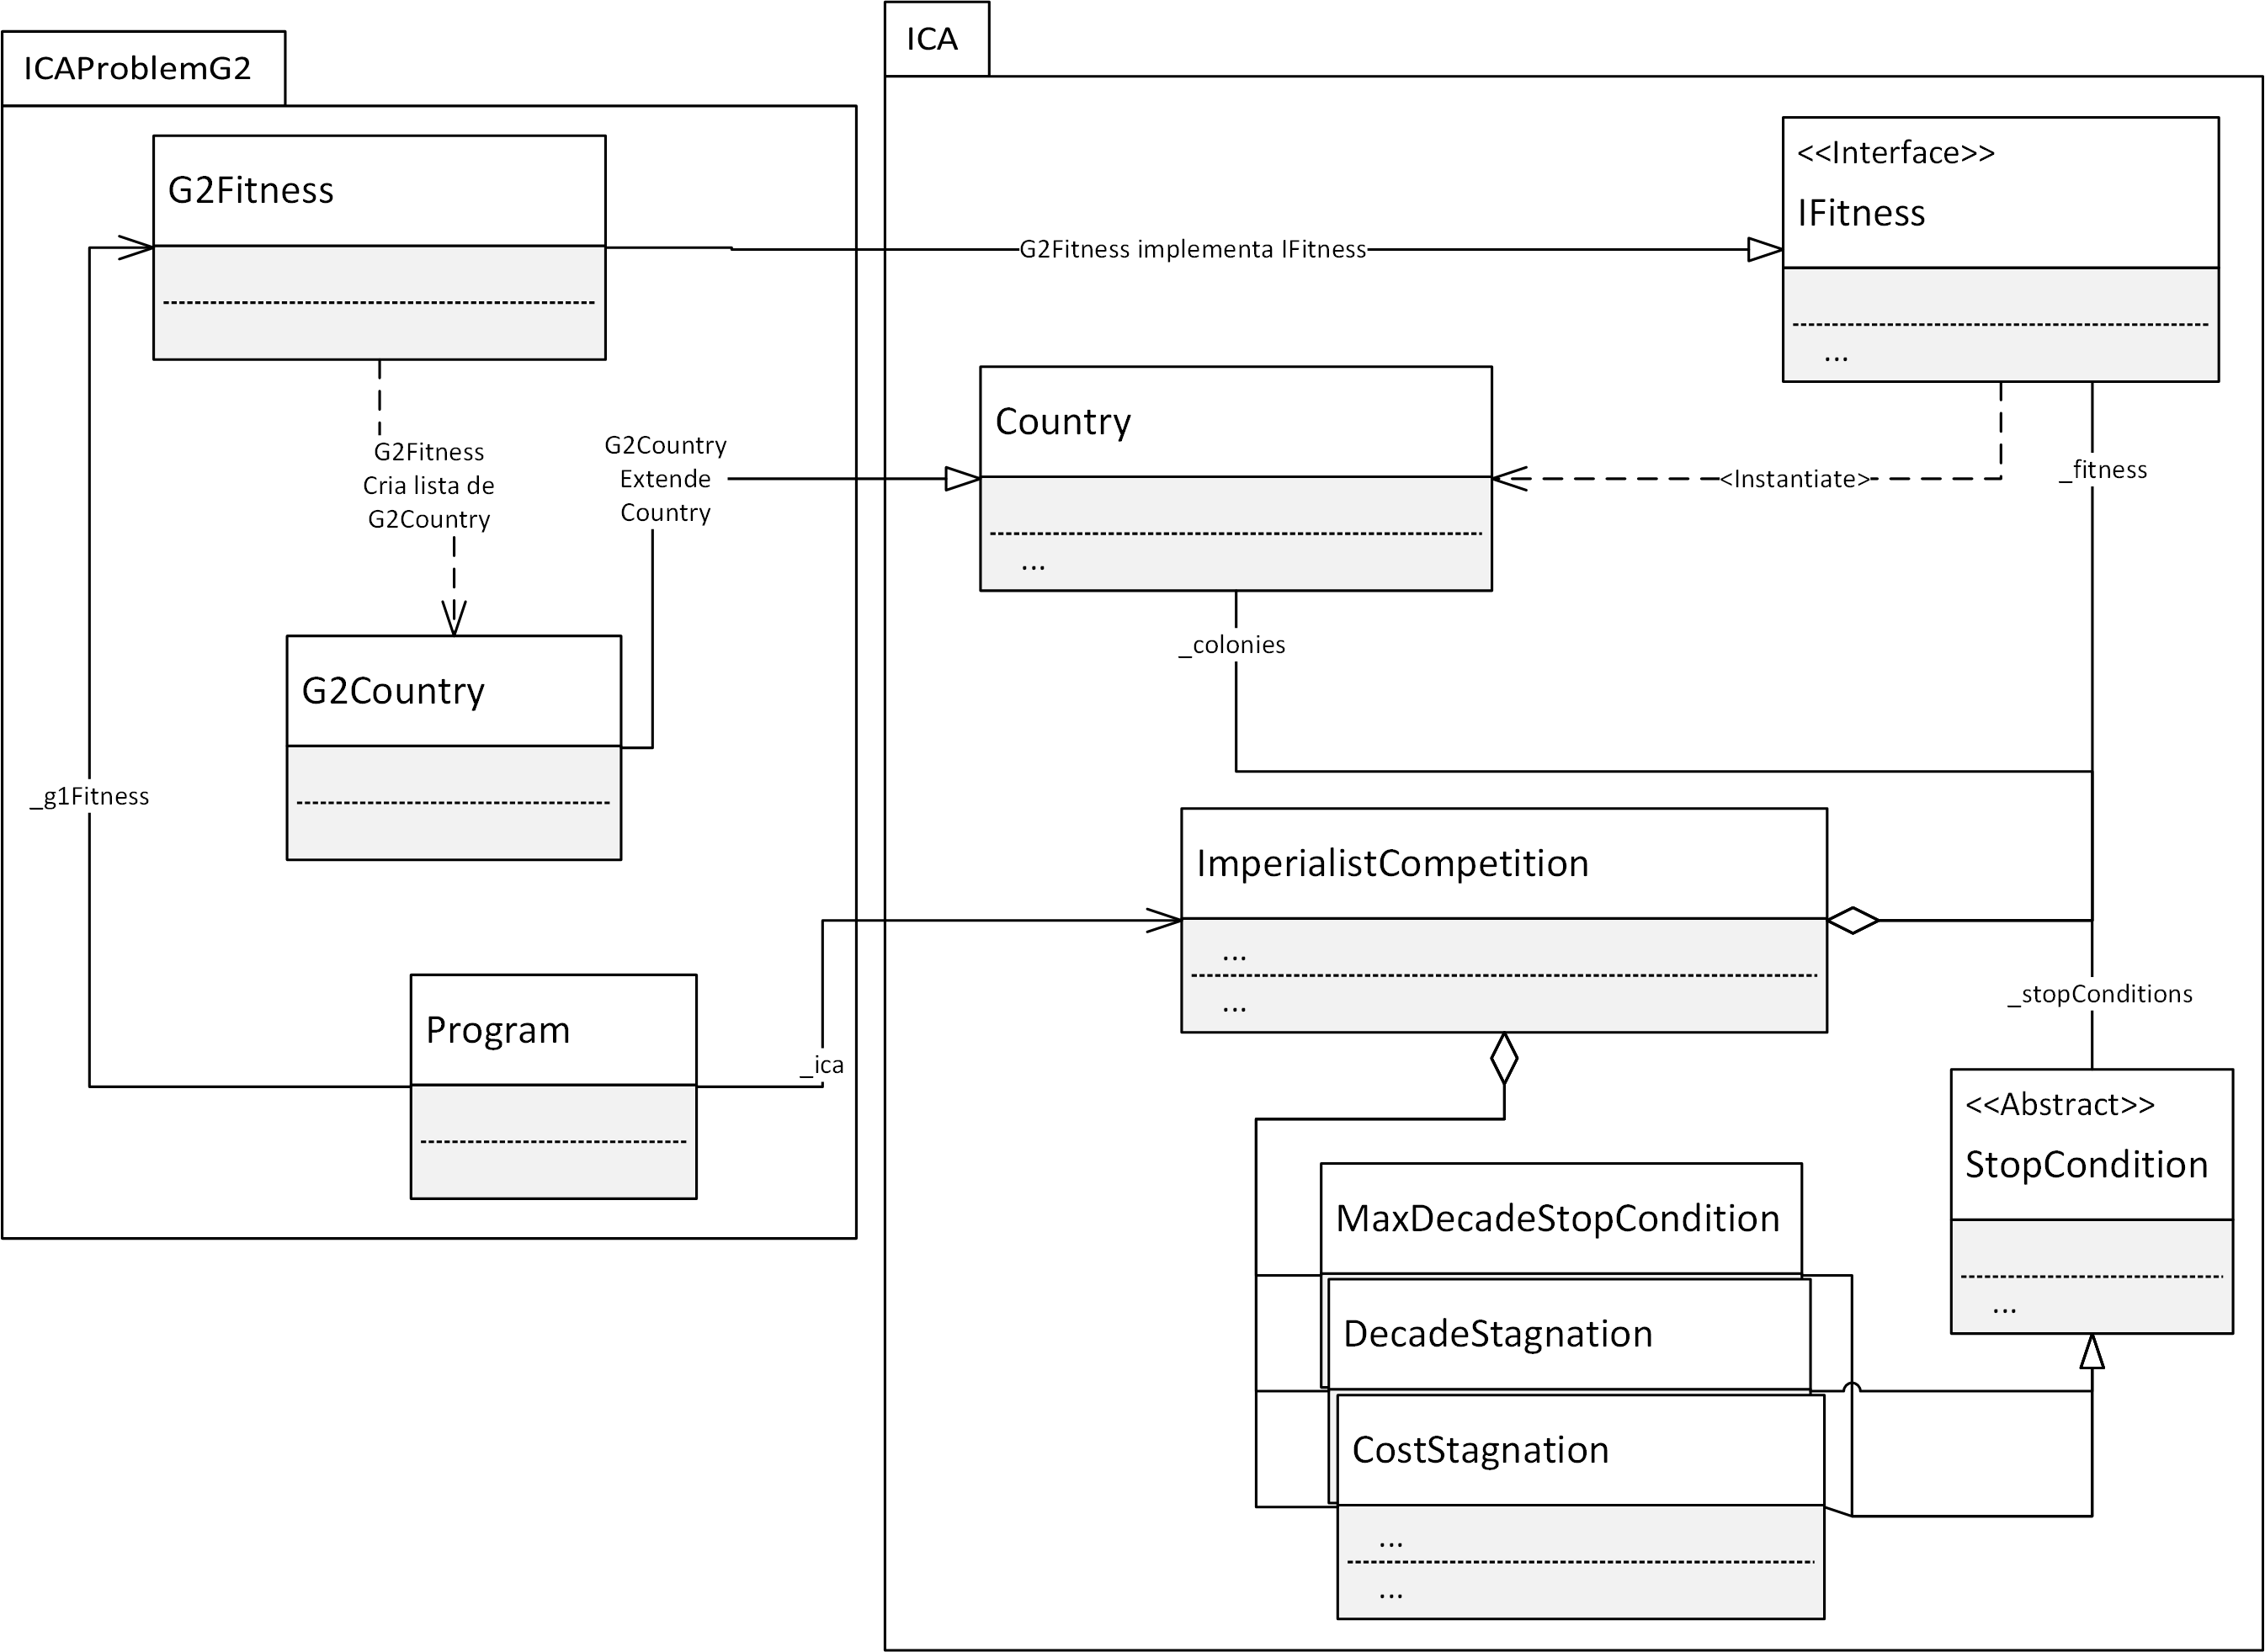
\includegraphics[scale=0.5]{Figuras/Problems-G2Model.png}
	\caption{Diagrama de classes simplificado do problema G2 }
	\label{fig:Problems-G2Model}
\end{figure}

Para que se alcance um resultado satisfatório a modelagem deste problema deve levar em conta, inicialmente, a ordem do filtro e os valores de cada elemento da matriz que representa este filtro. Então, um dos parâmetros definidos na modelagem do problema deve ser a ordem da matriz de convolução, que define quantos atributos os países terão.

Com a ordem estipulada, tem-se que a propriedade \emph{Dimensions} da classe \emph{G2Fitness} retorna a definição do número de dimensões do problema como sendo \(Dimensions = ordem * ordem\). Assim, com o número de dimensões estipulado, para o caso geral de \emph{ordem = n}, o vetor de atributos deve representar todos os elementos da matriz filtro em uma sequência unidimensional representada conforme a Figura \ref{fig:Problems-G2Vector}.

\begin{figure}[h]
	\centering
	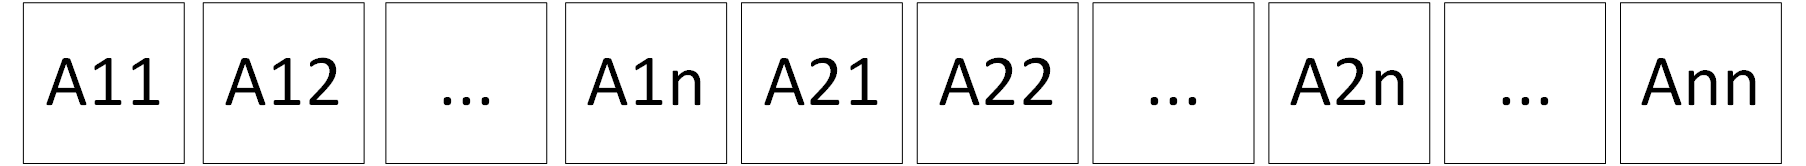
\includegraphics[scale=0.8]{Figuras/Problems-G2Vector.png}
	\caption{Vetor de atributos dos países do problema G2}
	\label{fig:Problems-G2Vector}
\end{figure}

Com o modelo do problema pronto, antes de implementar os métodos da interface \emph{IFitness} na classe \emph{G2Fitness}, estende-se a classe \emph{Country} para a classe \emph{G2Country}, que por sua vez sobrescreve o método \emph{RandomizeAttributes} para utilizar uma função randômica de distribuição normal (substituindo a distribuição anterior, que era uniforme), que por padrão tem \(\mu = 0\) e \(\sigma = 0.269\) (de modo que o valor aleatório retornado varie entre 0 e aproximadamente 1). Outra funcionalidade que a classe \emph{G2Country}  traz é a adição de uma propriedade para se armazenar o resultado que o método \emph{Eval} da classe \emph{G2Fitness} gera, de forma que se possa salvar esta informação durante ou depois do processamento do ICA.

O método \emph{Eval} da classe \emph{G2Fitness} é implementado para avaliar qual matriz de convolução presente em cada país é a que mais se encaixa na utilizada para gerar a imagem resultado (I') a partir da imagem original (I) conforme o Algoritmo \ref{alg:G2Problem}

\begin{algorithm}[h]
\SetAlgoLined
\KwData{
\\ \textbf{ref} element - A referência do país a ser avaliado
\\ \textbf{\emph{static}}  I - Imagem original
\\ \textbf{\emph{static}}  I' - Imagem resultado
}
\KwResult{ nenhum valor de retorno, pois altera-se diretamente na referência de element}
Transformar os atributos do país em uma matriz de convolução (M)\;
Efetuar a operação de convolução entre a imagem original (I) e a matriz de convolução (M), obtendo a imagem resultante (R) \;
Calcular a diferença absoluta entre todos os pontos da imagem resultante (R) e a imagem resultado (I'), e armazenar a soma em (d)\;
element.Cost = d\;
element.resultado = R\;
\caption{ Pseudocódigo método \emph{Eval} do problema G1.}
\label{alg:G2Problem}
\end{algorithm}

Durante os testes foi utilizada uma mesma imagem para dois filtros diferentes. Os dois filtros utilizados são o desfoque gaussiano e detecção de borda, apresentados respectivamente com sua aplicação na Figura \ref{fig:Problems-G2Convolution}.

\begin{figure}[h]
	\centering
	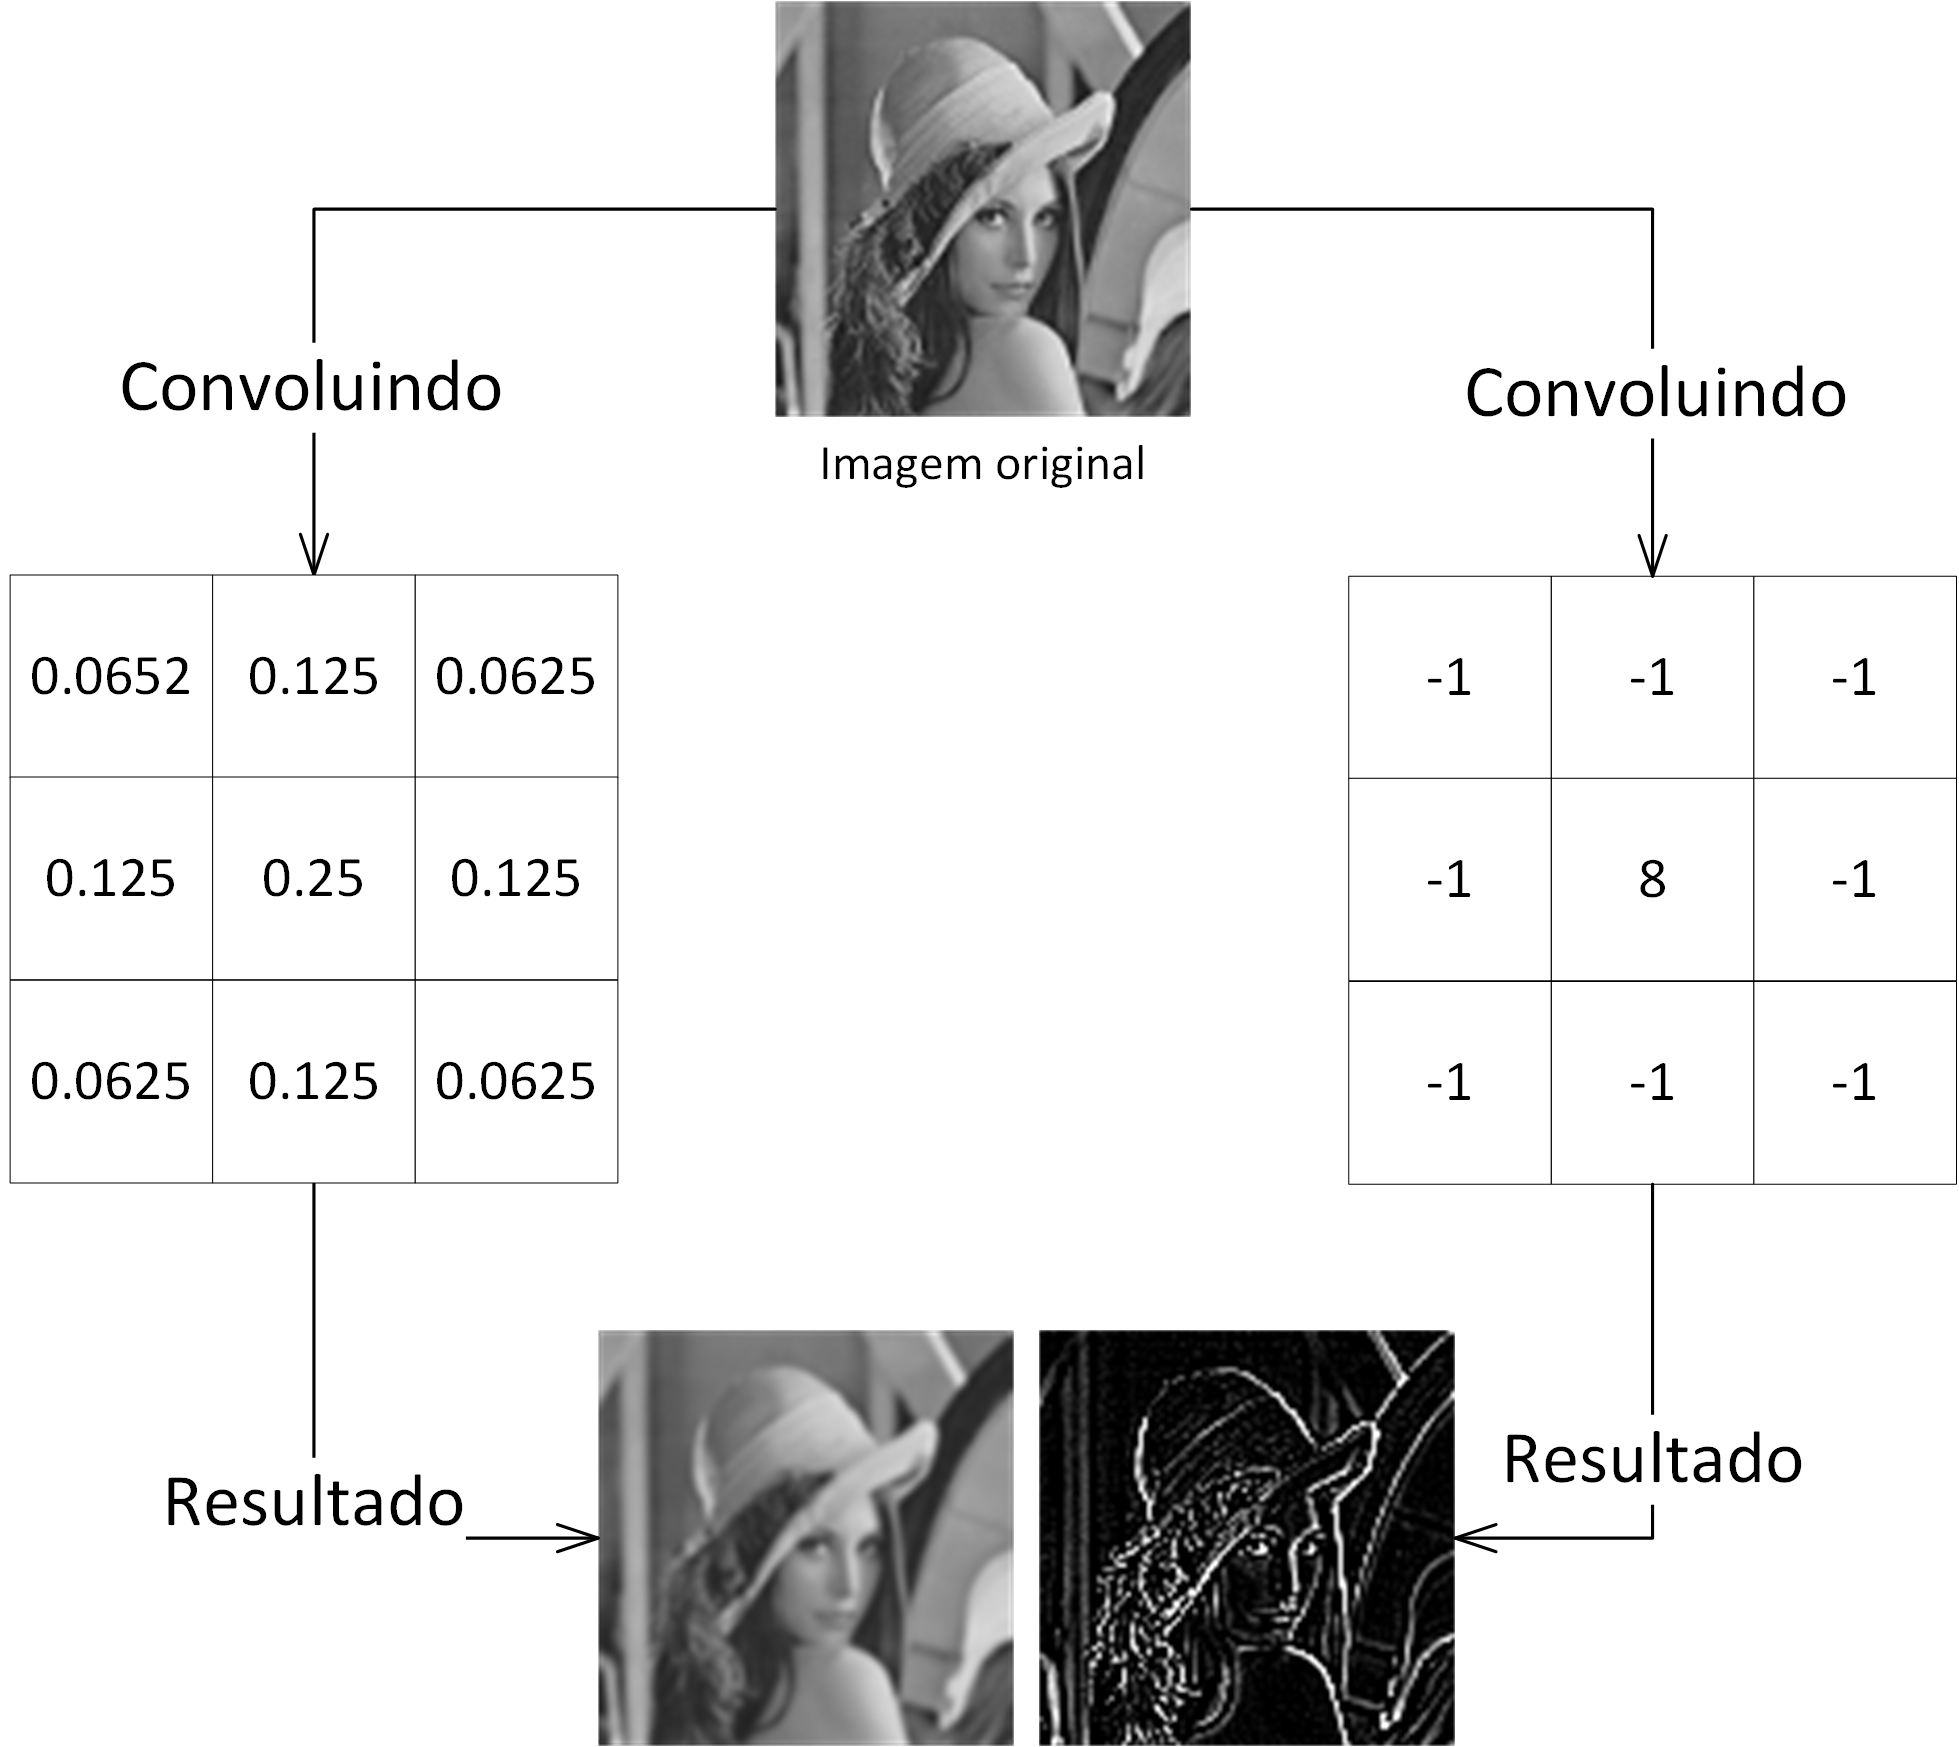
\includegraphics[scale=0.6]{Figuras/Problems-G2Convolution.png}
	\caption{Exemplo Problema G2}
	\label{fig:Problems-G2Convolution}
\end{figure}

Para que o ICA possa encontrar estes dois filtros, ambos tiveram como entrada inicial os mesmos parâmetros, diferenciando-se apenas na imagem resultado e nos limites dos atributos. Os parâmetros de entrada que que foram configurados na inicialização do ICA foram:

Total de países: 64, 

Número máximo de décadas: 2048, 

Taxa de revolução: 0.99, 

Taxa de decaimento de revolução: 0.9999, 

Coeficiente de assimilação: 2, 

Epsilon: 0.025, 

Porcentagem inicial de impérios: 0.15. 

Já os limites, para o filtro de desfoque gaussiano foi escolhido um intervalo entre 0 e 1 para todos os atributos, e para o filtro de detecção de bordas foi escolhido o limite entre -2 e 10 para todos os atributos.

Os demais valores foram mantidos como padrão e podem ser consultados no Anexo1

Os resultados apresentados pela busca de ambos os filtros foram muito bons, e se aproximaram muito do original, como mostrado a seguir na Figura \ref{fig:Problems-G2Results}.

\begin{figure}[h]
	\centering
	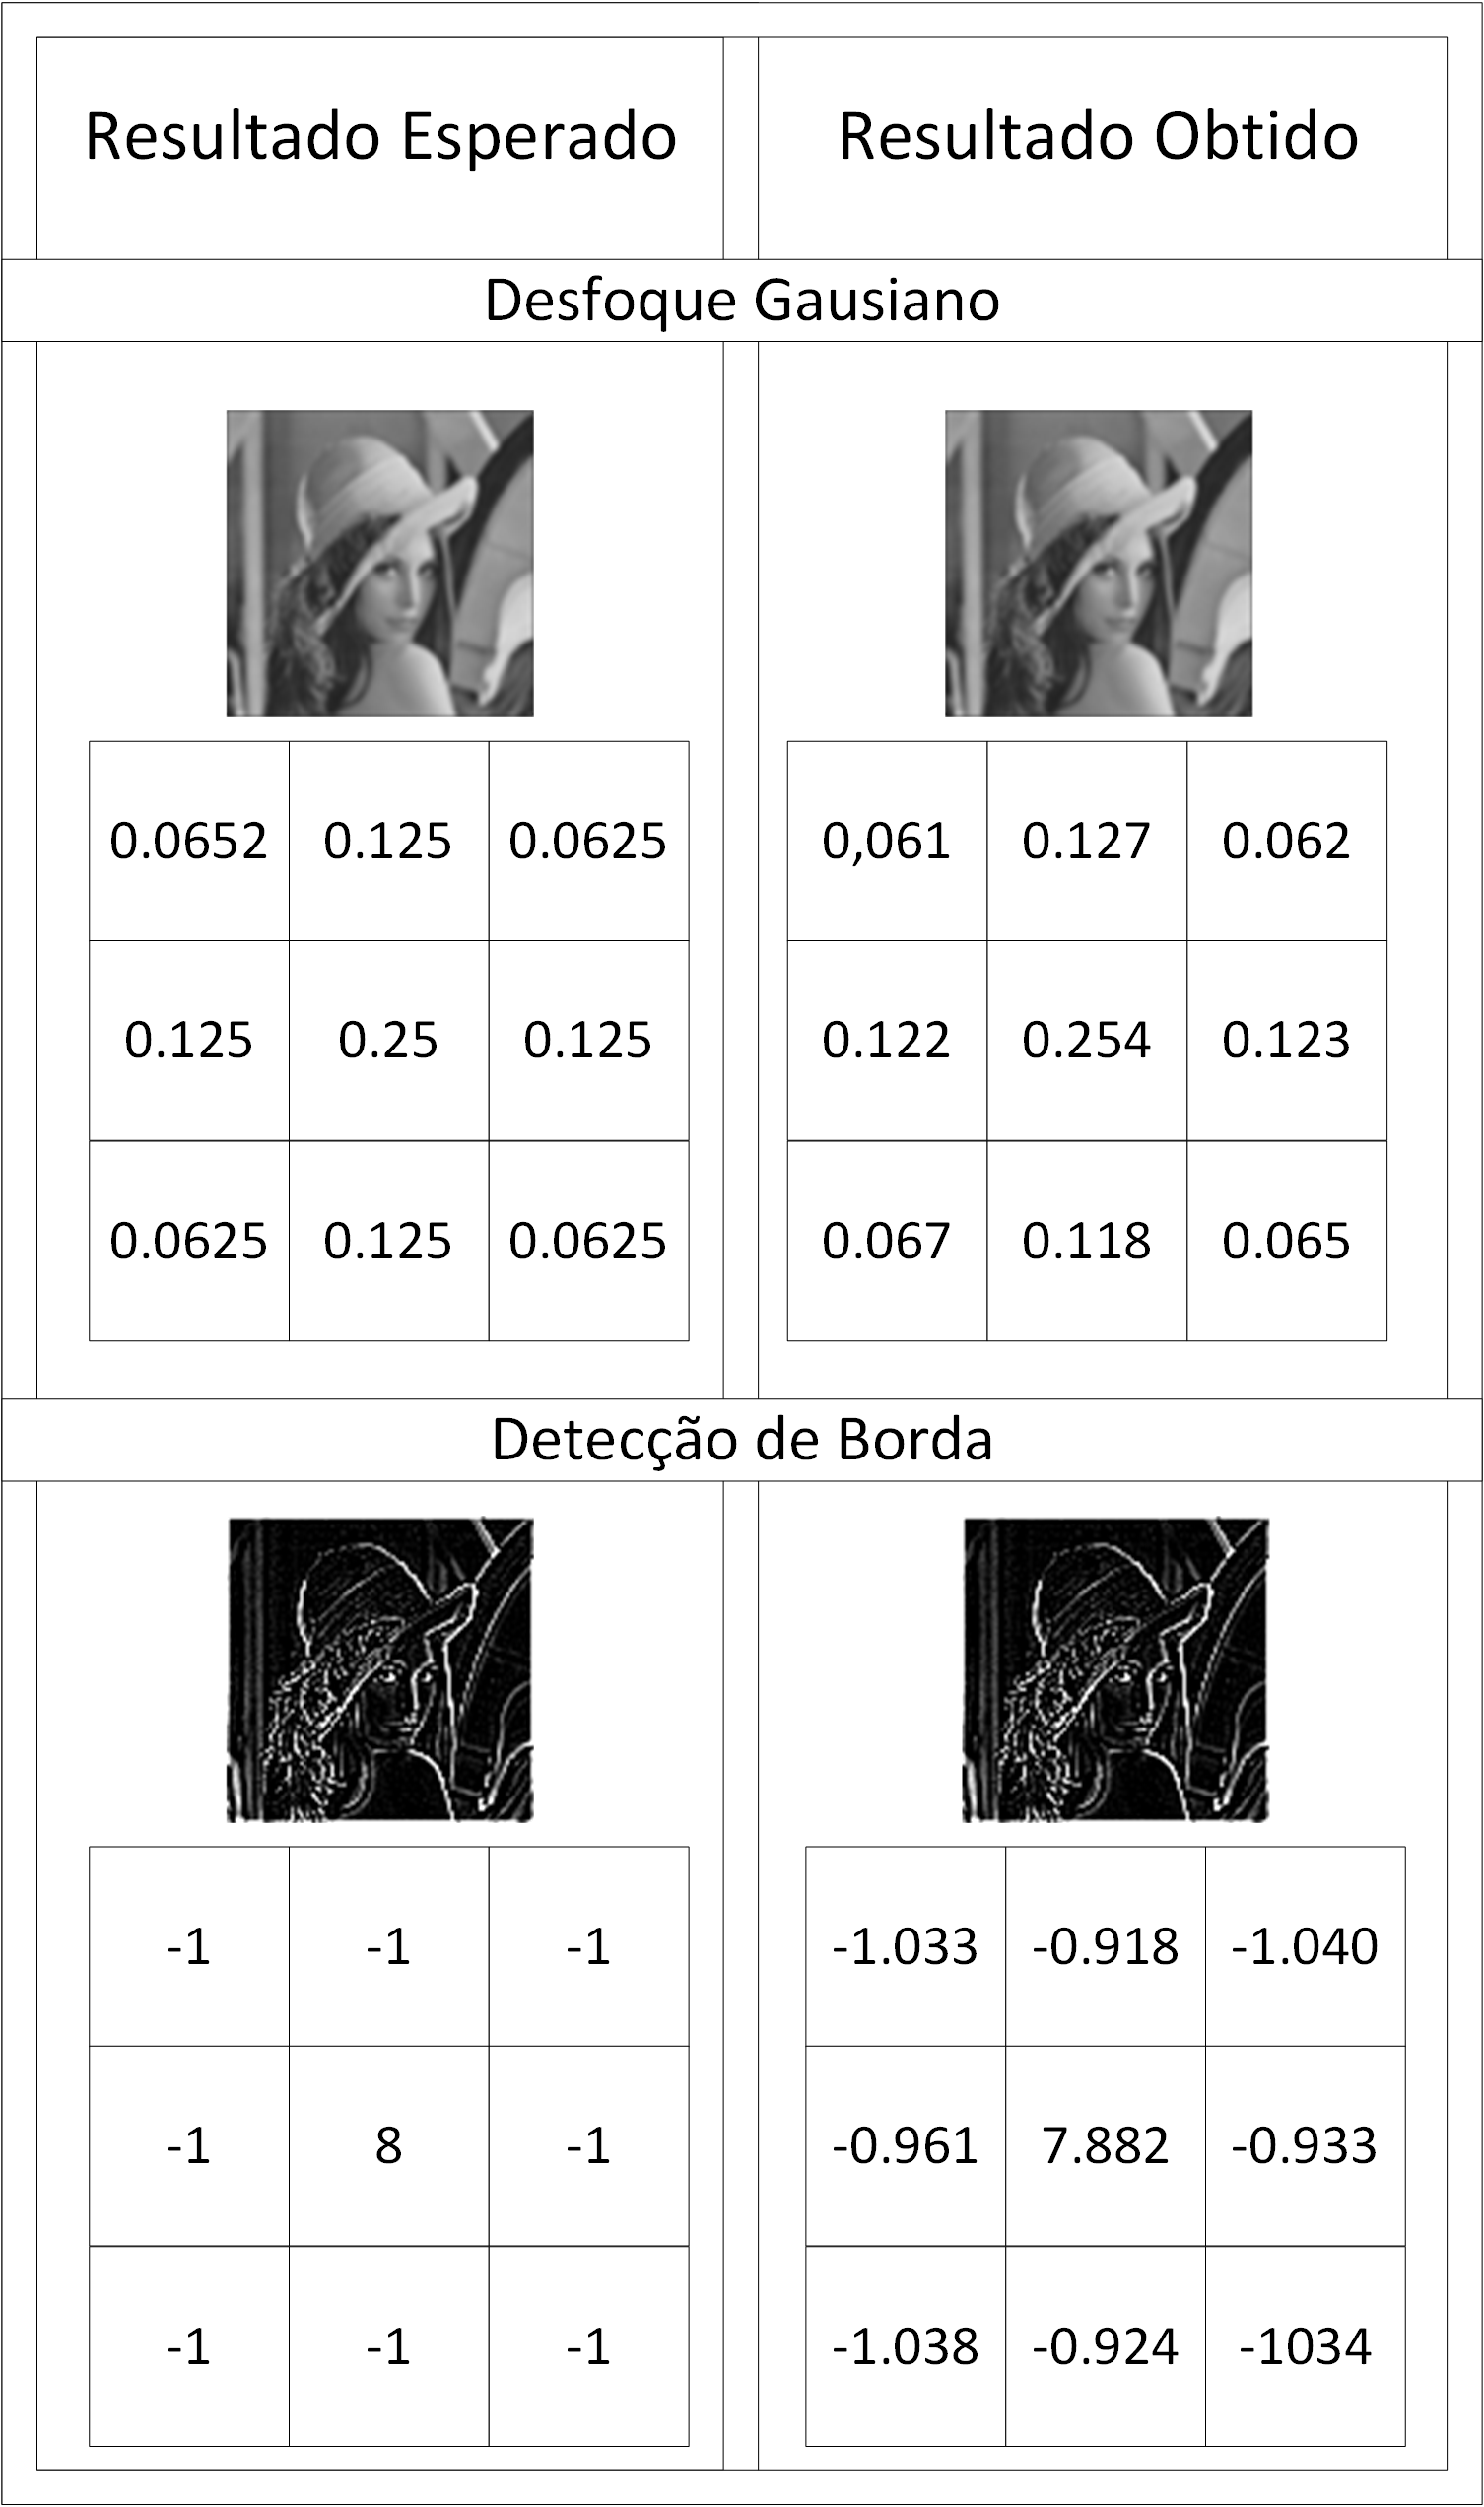
\includegraphics[scale=0.9]{Figuras/Problems-G2Results.png}
	\caption{Resultados do problema G2}
	\label{fig:Problems-G2Results}
\end{figure}

Observa-se que apesar dos resultados dos filtros não atingirem a exatidão, estes chegam muito próximo do resultado esperado e geram imagens indistinguíveis a olho nu. As imagens resultado possuem um erro percentual médio de 0.0471\% e 0.3342\% para as imagens originais geradas a partir do filtro de desfoque gaussiano e de detecção de bordas respectivamente.  

Assim concluímos os exemplos demonstrando a praticidade com que a generalização traz para a modelagem de problemas completamente diferentes, mantendo a estrutura principal do algoritmo inalterada, de modo a adicionar tais problemas como se fossem módulos encapsulados os quais são consumidos e processados pelo ICA.









\section{Análise da operação de movimento do ICA}

Antes de apresentar cada alteração na operação de movimentação, foi definido um problema que será usado como referência para ambientalizar e ilustrar o entendimento, tanto da operação de movimento citada originalmente, quanto das operações de movimento alteradas apresentadas neste trabalho. O problema P1 em questão refere-se a minimização da função esfera dentro de um intervalo fechado e bidimensional, como mostra a equação \ref{eq:ProblemP1-SphereFunction}.  

Serão apresentadas várias figuras contendo diversos elementos relacionados ao problema, de modo que a estrela vermelha representa a posição em que o país imperialista se encontra, os pontos azuis ligados por linhas representam uma colônia se movendo em direção ao seu país imperialista durante as décadas e a coloração do fundo da imagem, em escalas de cinza, é uma plotagem da função em questão, neste caso da função esfera, que encontra-se no espaço bidimensional dentro do intervalo \(\left[-10, 10\right]\) tanto para \(x\) quanto para \(y\). Esta função foi escolhida, além de ser bem comum, por ter seu mínimo global bem definido e único para este intervalo.

\begin{equation}
f(x,y) = x \cdot x + y \cdot y, \\ x:[-10,10], \\y:[-10,10]
\label{eq:ProblemP1-SphereFunction}
\end{equation}

Inicialmente é preciso entender o que ocorre durante o processo evolutivo do ICA, então, para estes exemplos a funcionalidade de possessão imperial, a qual ocorre quando uma colônia mais forte que seu país imperialista toma o poder para si, foi desabilitada (exceto alguns casos, detalhados mais adiante), de modo que quando uma colônia passar por uma posição de custo menor ela não tome o império para si, além disso, o valor de \(\beta\) utilizado é menor que 1, a taxa de revolução colonial fora configurada como 0, evitando que países tenham seus atributos sorteados novamente, e, por fim, o espaço de busca será explorado por apenas uma colônia junto de um país imperialista, que irão formar um império contendo apenas dois países. A posição inicial da colônia é definida como \((-8,-5)\) e a posição inicial do país imperialista é definida como \((-2,-2)\), mesmo sabendo que o ponto ótimo será o ponto \((0,0)\) e o número máximo de décadas é 40.

A forma como as colônias se movem em direção ao seu imperialista é definida pelo resultado de um valor aleatório proporcional a distância entre cada atributo da colônia em relação aos atributos do país imperialista, e de forma independente dos limites de cada dimensão, tal que, este valor aleatório altera cada atributo na mesma proporção. Assim, pode-se dizer que este valor aleatório representa o tamanho do ‘passo’ que uma colônia dará em direção ao seu país imperialista (lembrando que este valor aleatório é gerado uniformemente no intervalo \(\left[0,\beta\right]\) como mostra a equação \ref{eq:ica7}.


A Figura \ref{fig:Movimento_Linear} ilustra o movimento linear de uma colônia em direção ao seu país imperialista sem a adição de ruído no movimento. Este ruído no movimento se dá pela alteração de cada atributo da colônia somando um valor aleatório, gerado de forma uniforme, e chamado \(\theta\) como mostrado na equação \ref{eq:ica9}. Observe que não foi encontrado o melhor resultado, o qual estaria na posição \((0,0)\) para a solução do problema, apenas houve uma convergência para a mesma posição do império, pois o ruído fora desabilitado para este demonstração.

\begin{figure}[h]
	\centering
	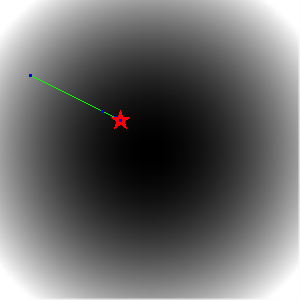
\includegraphics[scale=1]{Figuras/Movimento_Linear.png}
	\caption{Movimento Linear }
	\label{fig:Movimento_Linear}
\end{figure}

Como dito anteriormente, o movimento de uma colônia em direção ao seu país imperialista tem como objetivo principal explorar o espaço de busca para encontrar soluções melhores. O problema de se mover linearmente uma colônia em direção ao seu país imperialista, sem a adição de um ruído, é o mesmo que limitar a busca por soluções melhores dentro de problemas mais complexos, podendo, ao fim das décadas, não chegar ao mínimo global (solução ótima), como pode ser visto na Figura\ref{fig:Movimento_Linear}. Porém o fato da solução não convergir para o mínimo global não significa, neste caso, que a solução estagnou-se em um mínimo local, mas sim que o algoritmo é incapaz de evoluir para a melhor solução por não possuir recursos (adição de ruído durante o movimento) para isto. Então é interessante a adição de um ruído neste movimento, de forma que o espaço de busca seja melhor explorado pela colônia enquanto ela se movimenta em direção ao seu império, como mostra o item \(a\) da Figura \ref{fig:Movimento_Original}. No capítulo \ref{Metodologia} este ruído é definido por \(\theta\), que define um intervalo para a geração de um número aleatório dentro do intervalo \( \left[ -\gamma,\gamma \right]\) que é adicionado a cada atributo. 

O grande problema neste método de inserção de ruídos da forma como é apresentado é a não garantia de proporcionalidade em relação ao espaço de busca de cada atributo, podendo, em um problema mais complexo e com limites diferentes para cada atributo, ter o ruído variando demais em uma dimensão com limites mais apertados, mas ser insignificante em limites de intervalo muito amplo. Além de que com a adição de ruído desta maneira não é possível que a convergência para o cenário ideal (todas as colônias na mesma posição que seu país imperialista ) ocorra.  Os três primeiros itens da Figura \ref{fig:Movimento_Original} \((a, b, c)\), representam o movimento colonial tendo os ruídos definidos com \(\gamma\) valendo respectivamente \(\left(\frac{\pi}{4}\right)\), como descrito por \citeauthor{atashpaz2007imperialist} em \cite{atashpaz2007imperialist}, \(\left(\pi\right)\) e \(\left(4\cdot \pi\right)\). Observa-se que para o item \(a\), existe uma quantidade de ruído pequena, que é aceitável, e que poderia estar levando o império em direção ao mínimo global caso o mecanismo de tomada de poder estivesse habilitado. Já os itens \(b\) e \(c\) apresentam um significativo aumento no ruído, podendo, também, levar a melhor solução, porém esta variação é muito grande e, consequentemente, faz com que a busca pela solução ótima tenda a ser mais aleatória do que direcionada, podendo fazer com que a solução ótima nunca seja atingida.  

\begin{figure}[h]
	\centering
	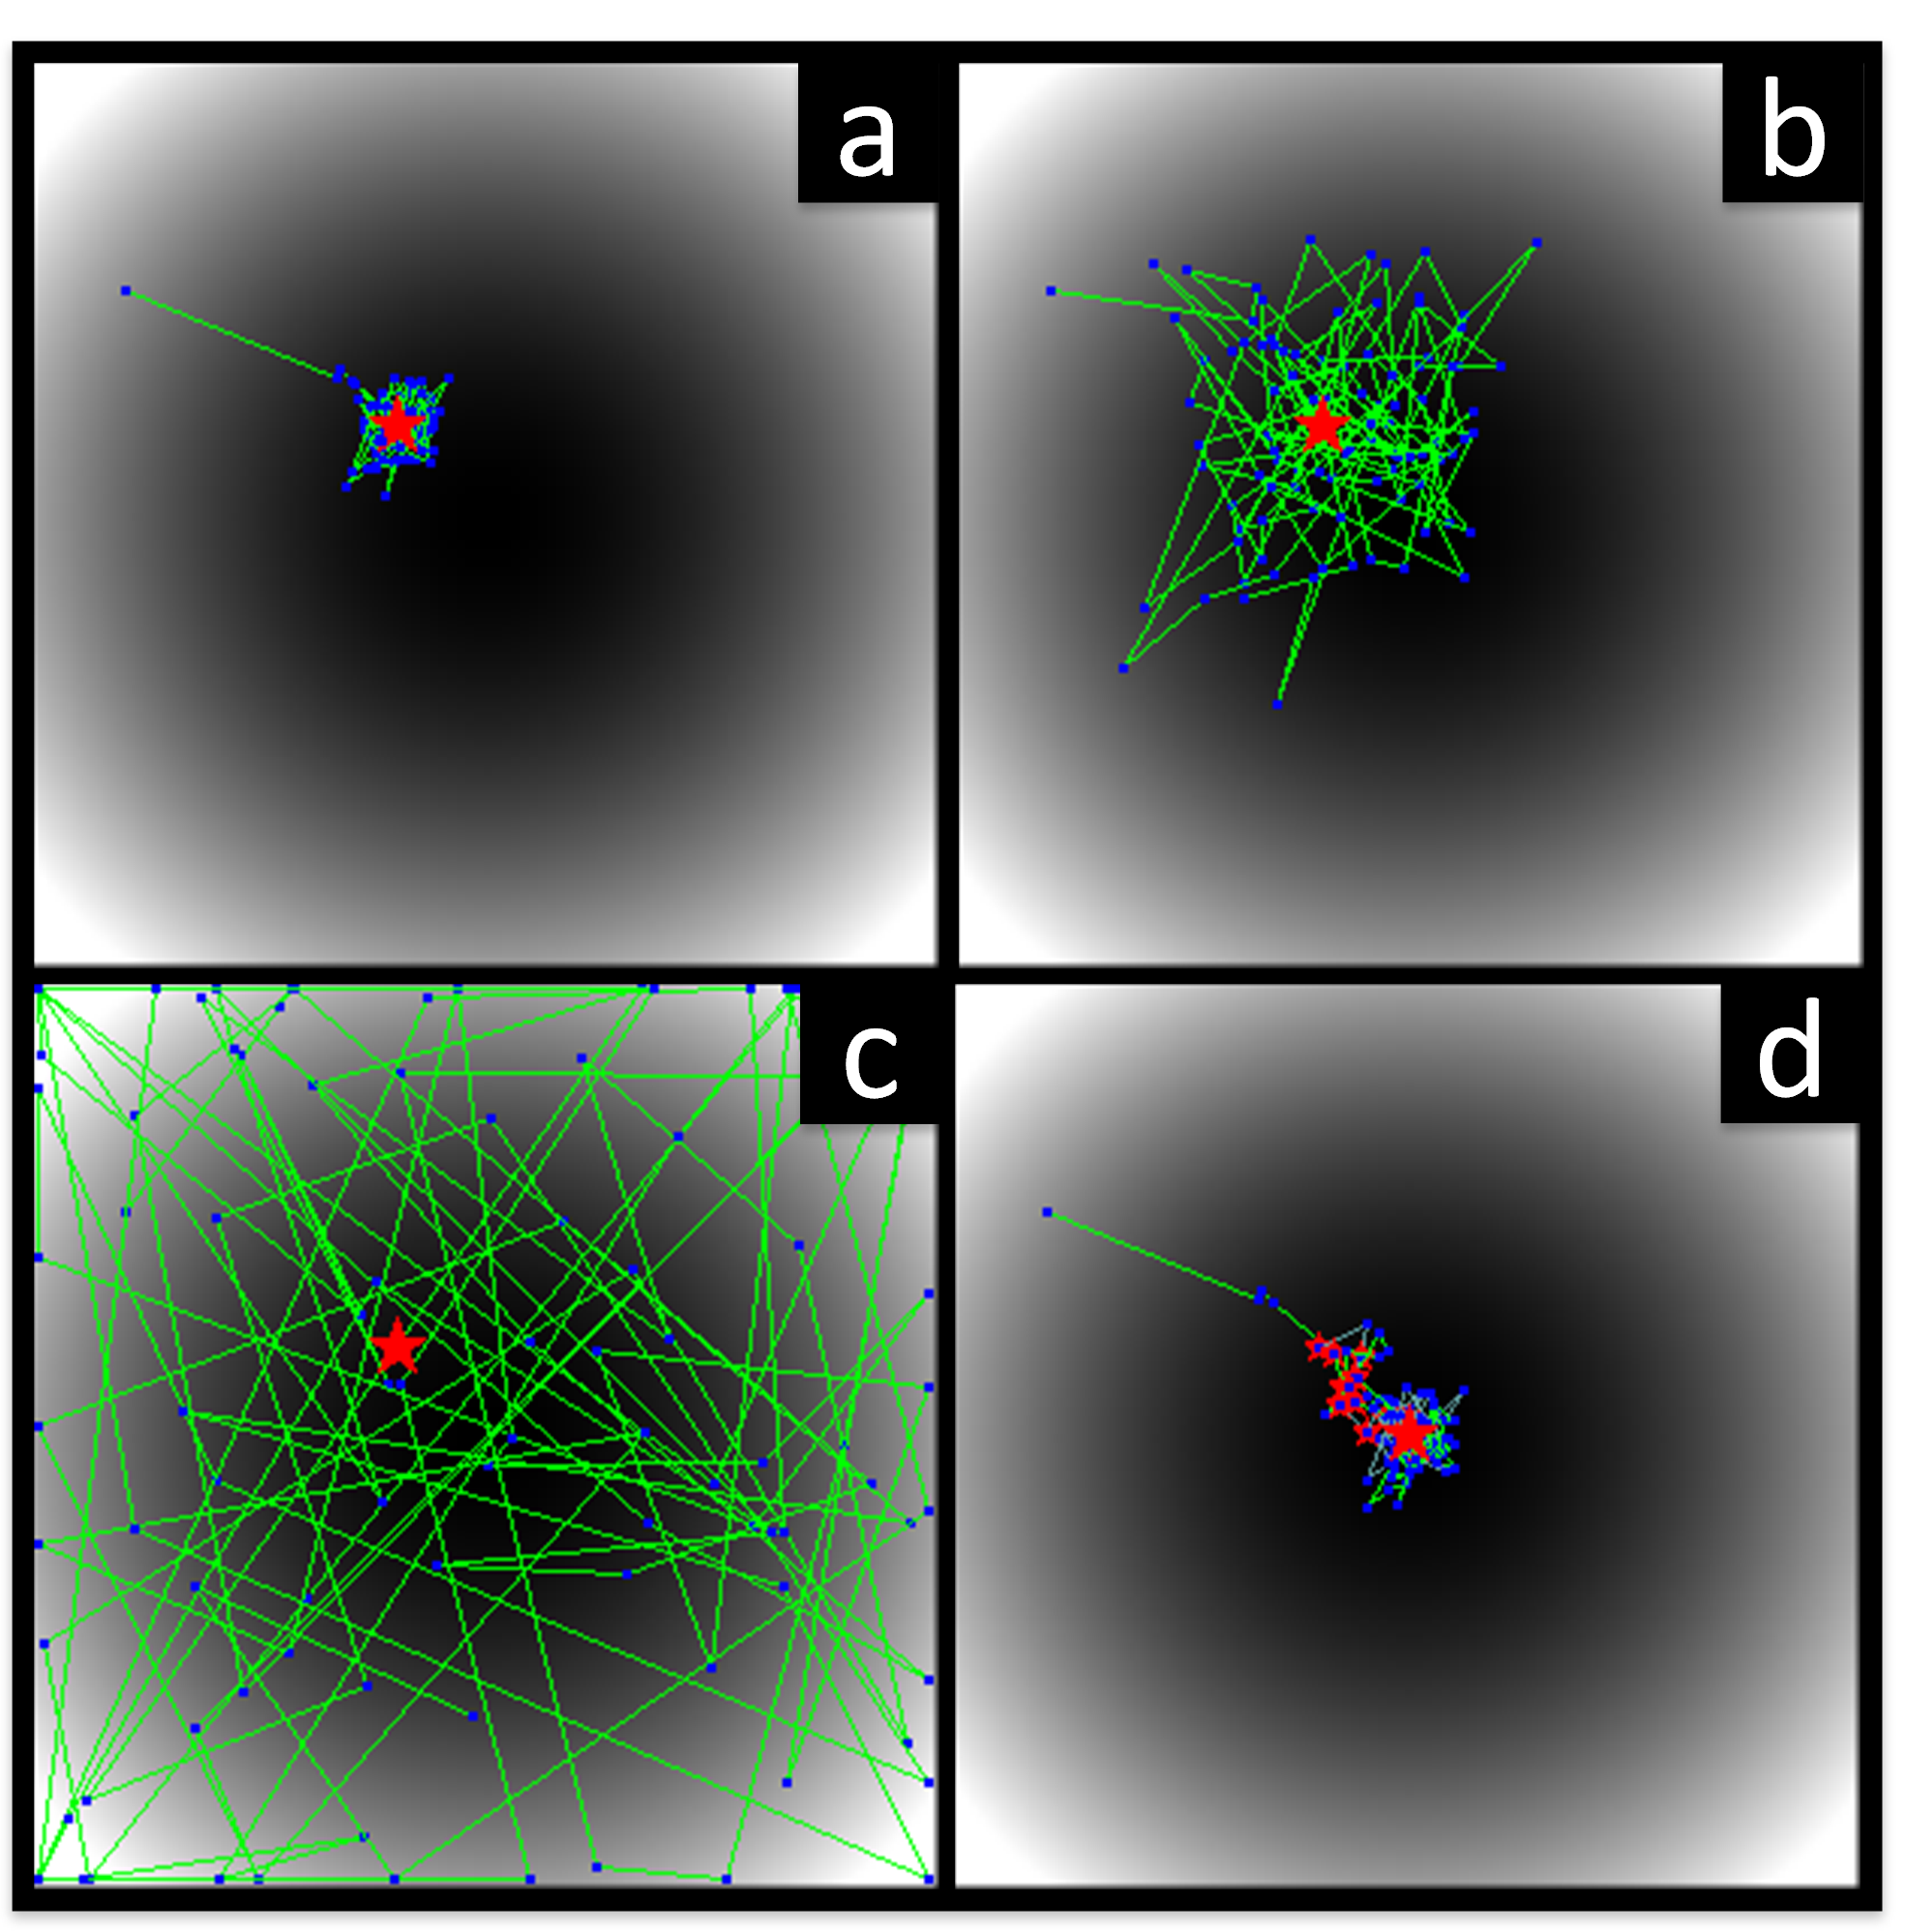
\includegraphics[scale=0.9]{Figuras/Movimento_Original.png}
	\caption{Movimento Original }
	\label{fig:Movimento_Original}
\end{figure}

O item \(d\) da Figura \ref{fig:Movimento_Original} apresenta o resultado do mesmo cenário do item \(a\), porém com a operação de possessão imperial habilitada. Na imagem, as estrelas menores representam os impérios durante as décadas, e a estrela maior representa a posição do império na última década. Observa-se que com a adição do ruído, houveram diversas trocas pelo controle do império entre os países competidores durante as décadas, até a solução convergir para o mínimo global. Outro fato interessante é que neste caso, o valor do ruído levou a um bom tempo de convergência, porém se a operação de possessão imperial tivesse sido habilitada no item \(c\), por exemplo, como mencionado anteriormente, o algoritmo levaria muito mais tempo para encontrar a melhor solução para este problema, pelo fato do ruído estar influenciando demais na definição do passo, que agora passa a ser menos direcionado e mais aleatório. 

A movimentação direta da colônia em direção ao seu país imperialista, isto é, sem adição de ruído, apesar de explorar menos o espaço de busca, converge mais rapidamente para seu império, podendo fornecer uma solução próxima da solução ótima. Por outro lado, quando se adiciona o ruído na movimentação, existe uma maior chance de que a colônia encontre melhores soluções do que a apresentada por seu país imperialista, podendo assim, esta colônia se tornar o centro do império. Esta operação ocorrendo diversas vezes leva os países deste dado império a se moverem para a melhor posição dentro do espaço de busca, de forma que ao fim, ou até mesmo antes do processo evolutivo terminar, se tenha a melhor solução em mãos. Então nota-se uma grande importância na adição de ruído, porém, da forma como é apresentado e calculado, quando um problema apresentar limites de tamanho diferentes, o ruído pode acabar prejudicando a otimização, a velocidade de convergência ou precisão do resultado na busca pela melhor solução.

A partir desta análise, foi possível criar novas formas de movimentação e verificar qual destas seria o melhor modo de mitigar os problemas trazidos com a adição de ruídos na movimentação. Assim foram concebidos os modelos:
\begin{itemize}
\item Movimento Refinado,
\item Visão imperial distorcida e 
\item Combinação de ambos.
\end{itemize}







\subsection{Movimento refinado}

O movimento refinado foi concebido com o intuito de solucionar o problema do movimento Original, o qual tem a geração de ruído fixa, e não proporcional aos limites do problema caso e as dimensões tenham limites diferentes para cada atributo. Então, a proposta é manter o ruído, porém este deve ser proporcional aos limites de cada dimensão. O fluxograma apresentado na Figura \ref{fig:Fluxograms-ColinyEmpireMovement} Original ICA demonstra a ordem em que ocorrem o cálculo dos valores que irão compor os novos atributos de uma dada colônia para o movimento original descrito anteriormente, sendo, o cálculo tamanho do passo \(x\) de cada atributo, calculado com o mesmo valor aleatório \(CoefAssimilação\) para todos os atributos, e quando é multiplicado pela distância, se torna proporcional aquele atributo. E antes de atribuir o novo valor a cada atributo, adiciona-se o valor de ruído aleatório. Assim define-se o valor final de cada atributo como apresentado pela equação \ref{eq:ica9}
	
\begin{figure}[hp]
	\centering
	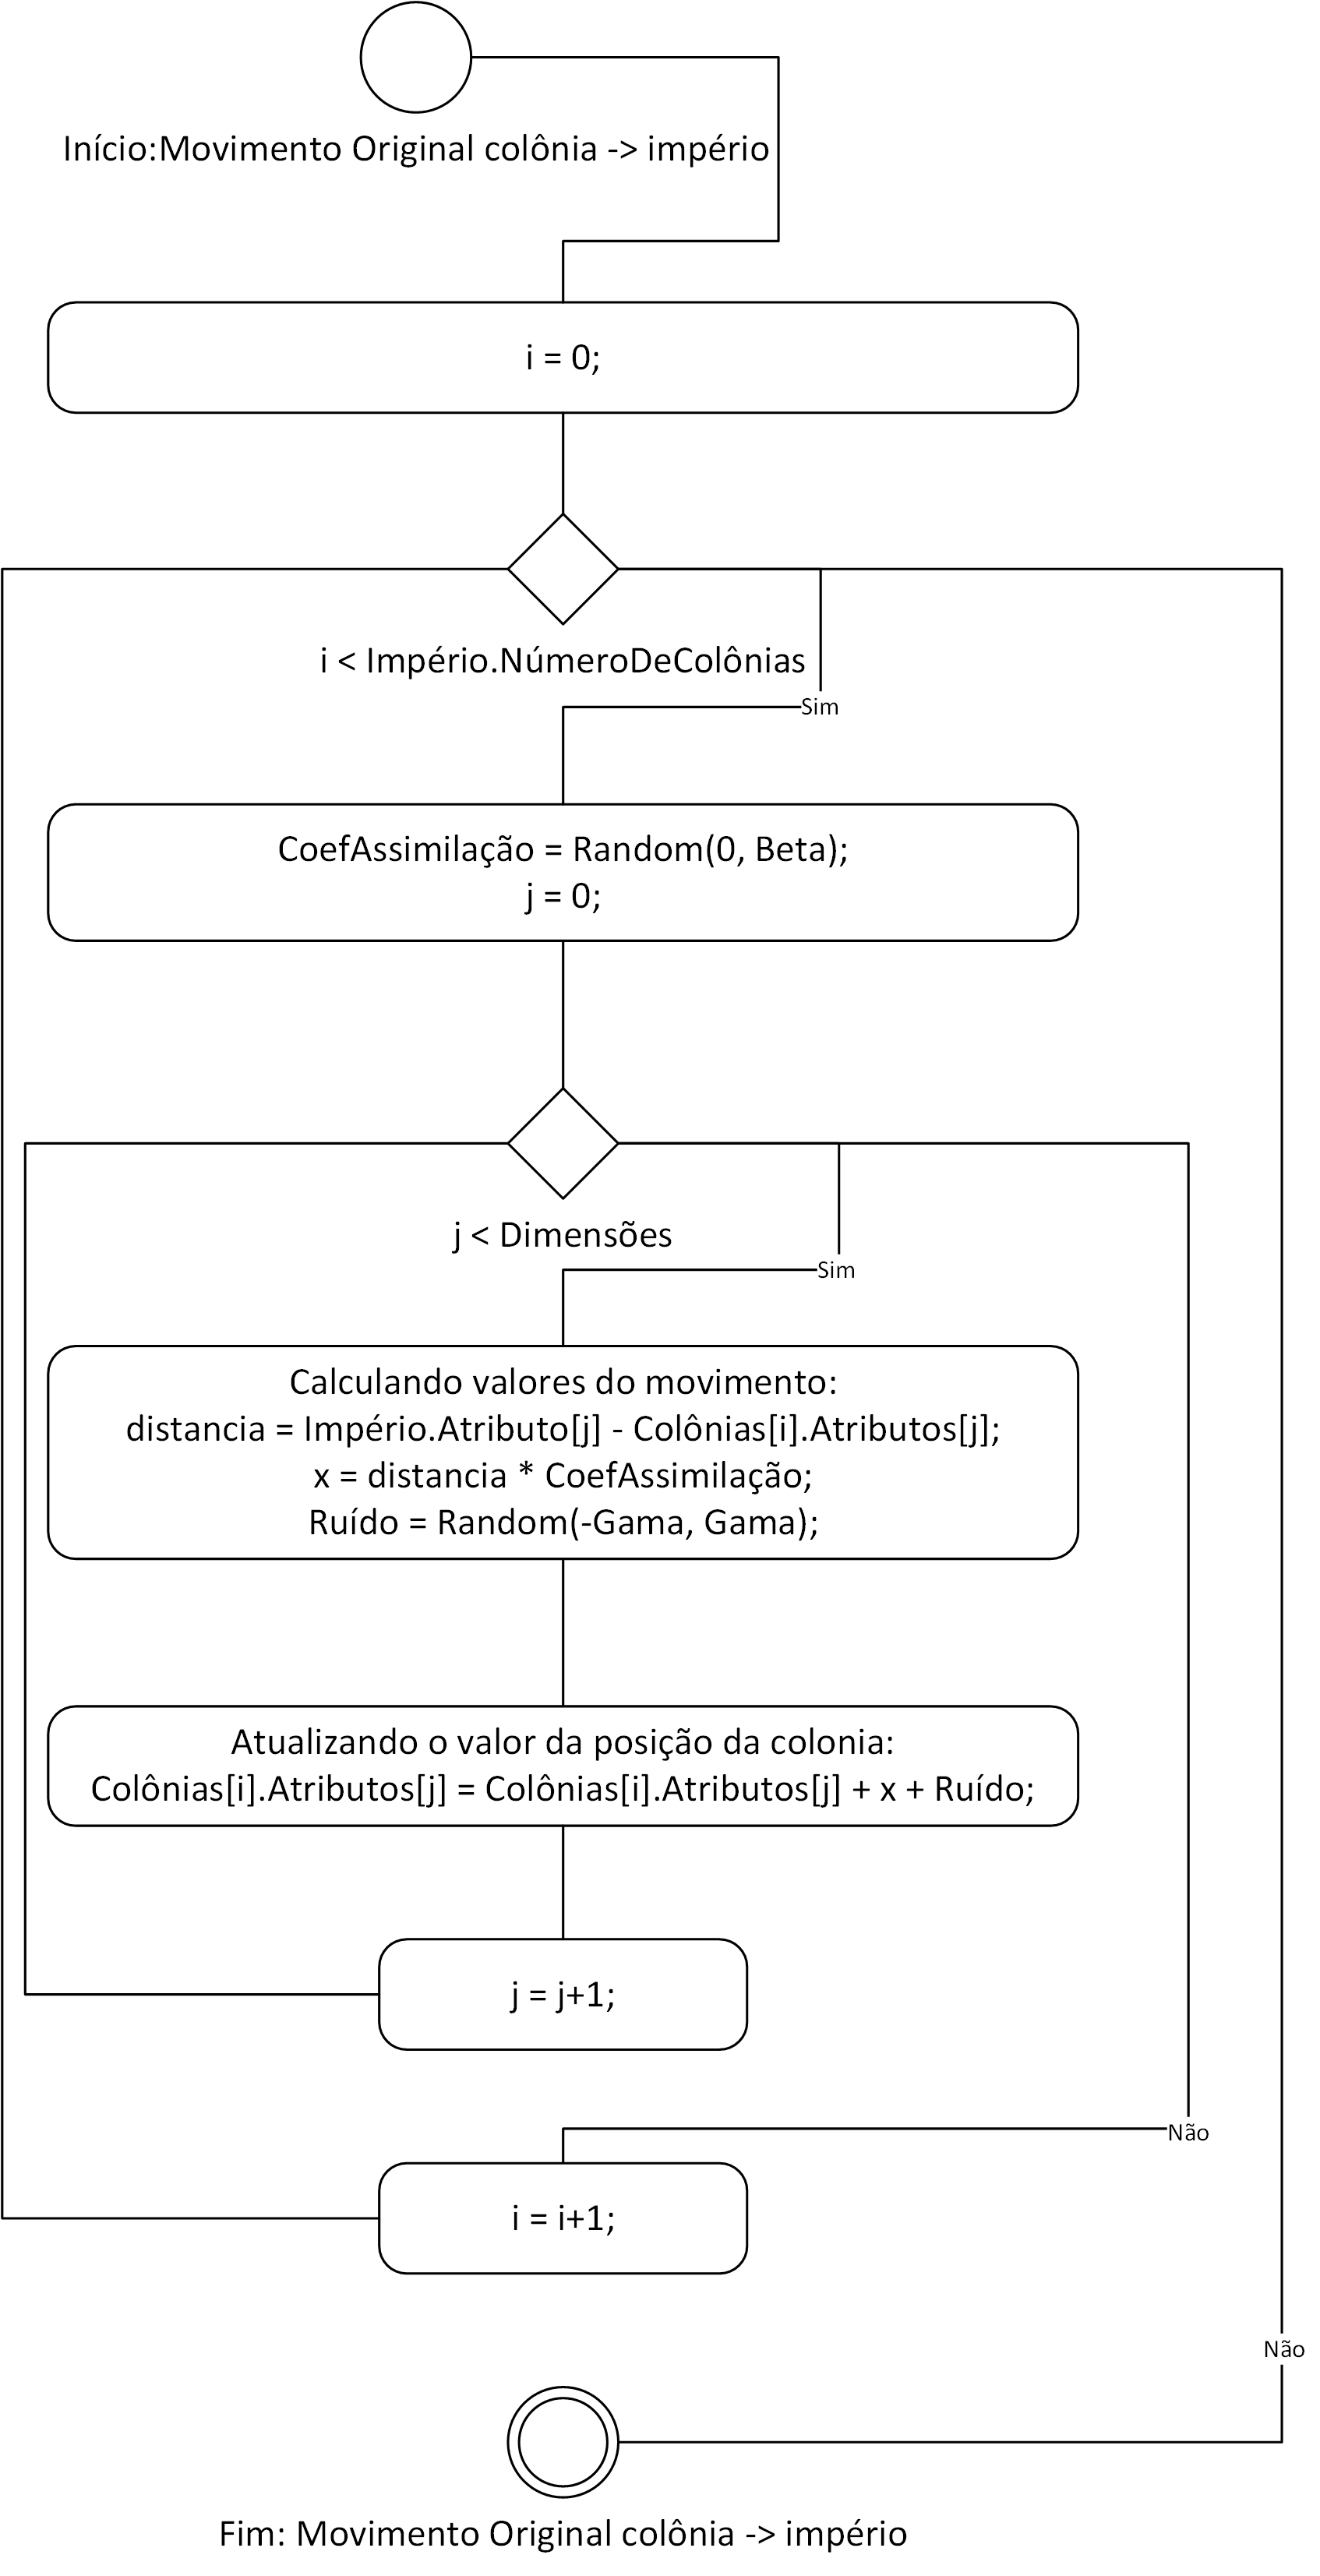
\includegraphics[scale=0.7]{Figuras/Fluxograms-ColinyEmpireMovement.png}
	\caption{Fluxograma Movimento Original ICA }
	\label{fig:Fluxograms-ColinyEmpireMovement}
\end{figure}	

	O método refinado de movimentação então, altera apenas o valor \(\theta\) de ‘Ruído’, que originalmente é calculado como um valor aleatório distribuído normalmente entre o intervalo \(\left[-\gamma, \gamma\right]\), que agora passa a ter uma estrutura dependente dos valores que definem os limites mínimo e máximo para uma dada dimensão e consequentemente do tamanho do espaço de busca, e de um valor de intensidade de ruído, que é um valor de controle, usado para definir o quanto de ruído, proporcionalmente ao espaço de busca, se deseja ter. Assim, este método adiciona uma nova propriedade de controle ao ICA, e troca a equação \ref{eq:ica8} que se resume em:
    
    \[\theta = URand(-\gamma, \gamma);\]
    
pela equação \ref{eq:refined}:

\begin{equation}
\label{eq:refined}
\begin{split}
\theta = 
& TriangularRand(MinBounds[i], MaxBounds[i], dist) \cdot \\ 
& \left(\frac{dist}{TamanhoEspaçoDeBusca[i]} + p \right);
\end{split}
\end{equation}

Sendo a função \(TriangularRand\) uma função que retorna um valor aleatório distribuído triangularmente entre \(MinBounds[i]\) e \(MaxBounds[i]\), e com moda sendo o valor \(dist\) entre o país imperialista e a colônia (observe na figura \ref{fig:Movimento_Original} que não é apenas usado o valor do módulo da distância, mas sim o vetor distância unidimensional, onde o sinal representará o sentido do vetor). O valor \(p\) é o que define a proporção do ruído, então se \(p\) for definido com o valor de 0.4, o ruído gerado ficará em torno de 40\% do tamanho do espaço de busca de cada dimensão para quando a distância entre o império e a colônia for próxima ou igual a zero. O fator \(\left(\frac{dist}{TamanhoEspaçoDeBusca[i]}\right)\) serve para potencializar o valor de \(p\) quando a distância entre a colônia e o império for grande, porém tende a zero quando o império e a colônia se aproximam, o que anularia o ruído, porém soma-se \(p\) justamente para manter o ruído na proporção desejada.

	A função \(TriangularRand\) tem um comportamento muito útil para esta alteração no modo de movimento justamente por gerar os valores, primeiro dentro do intervalo desejado e segundo por gerar tais valores aleatórios tendendo para um valor de moda definido, assim, pode-se gerar valores aleatórios dentro dos limites da dimensão e com a moda sendo a distância entre a colônia e o país imperialista, o que implica que a maior parte do ruído é gerado com mais chances de estar mais próximo ao império, aumentando a velocidade de convergência ao mesmo tempo que mantém uma pequena chance de ruídos mais intensos. A Figura\ref{fig:RandomTriangular-White} abaixo representa um histograma de três sequências de 1000 valores gerados por esta função no intervalo \(\left[0,1\right]\) e de moda 0, 0.5 e 1 respectivamente. Observa-se então, que existirá uma chance muito maior de que os valores aleatórios gerados pelo ruído estejam mais próximos da distância percorrida, mantendo um forma de controle sobre o ruído gerado e no caso, quando mais a distância diminui menor também será a chance de existirem ruídos mais intensos. 
	
	Apenas com o uso da função que gera valores aleatórios de distribuição triangular, já adiciona uma forma de ruído proporcional ao espaço de busca, porém ela ainda gera valores que podem levar a colônia para qualquer posição do espaço de busca aleatoriamente, quando a colônia estiver muito distante do império, fazendo com que a otimização fique muito mais aleatória do que direcionada. Então definiu-se \(p\) como sendo um valor definido dentro do intervalo \(\left[0,1\right]\) o qual soma-se com o valor proporcional da distância em relação ao espaço de busca \(\left(\frac{dist}{TamanhoEspaçoDeBusca[i]}\right)\), que então multiplica o valor gerado aleatoriamente com distribuição triangular entre os limites da dimensão e com moda como sendo a distância entre o atributo da colônia e do império nesta mesma dimensão, tornando este ruído limitado proporcionalmente a uma porção do espaço de busca. 
    
\begin{figure}[H]
	\centering
	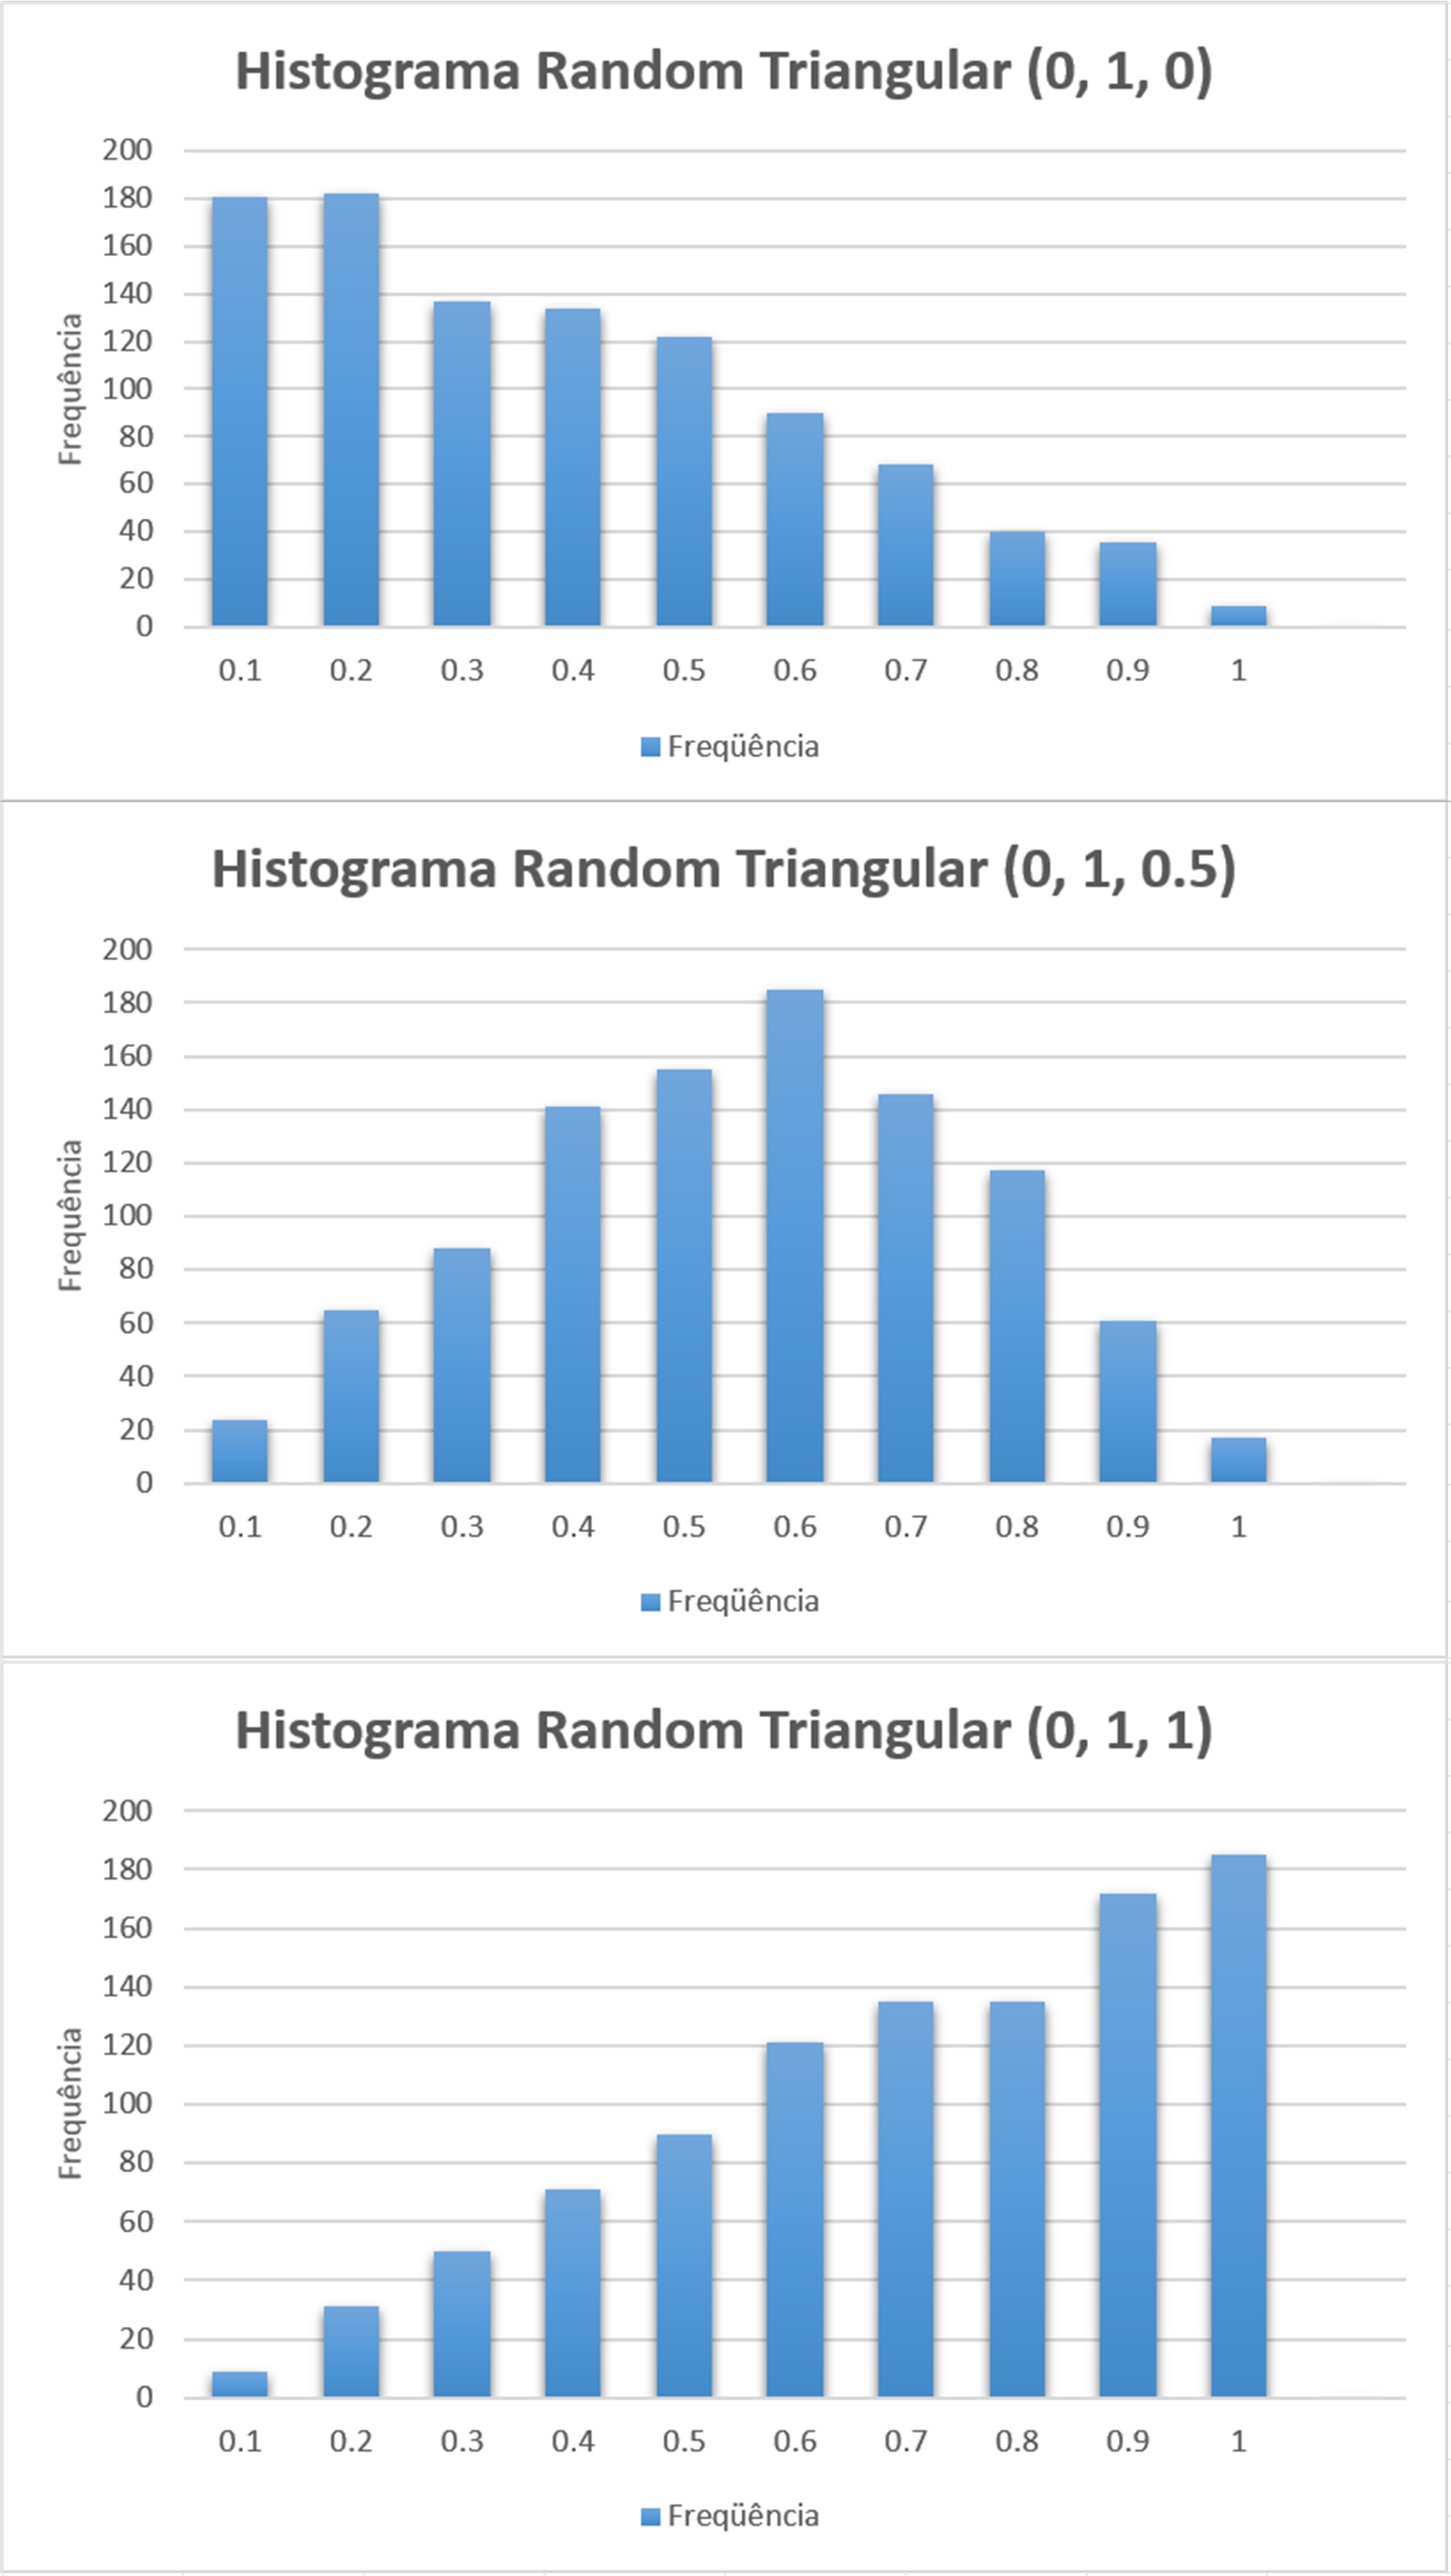
\includegraphics[scale=0.55]{Figuras/RandomTriangular-White.png}
	\caption{Random Triangular}
	\label{fig:RandomTriangular-White}
\end{figure}

A Figura\ref{fig:Movimento_Refinado}, analogamente a Figura\ref{fig:Movimento_Original}  apresenta 4 configurações diferentes para a busca da melhor solução, na qual as três primeiras são com a operação de possessão imperial desabilitada e a última tem esta funcionalidade habilitada. Observa-se que as imagens são muito parecidas, portanto agora existe um controle muito mais preciso sobre a intensidade  do ruído a ser gerado, sendo que os valores para p foram de 0.1, 0.4 e 0.8 para os resultados \(a\), \(b\) e \(c\) respectivamente, e em \(d\) foi utilizado p = 0.1 e a operação de possessão imperial estava habilitada. Em comparação com o modelo original, ao utilizar o método refinado, ocorrem aproximadamente 10\% mais possessões imperiais, ou seja, aumentaram-se as chances de uma colônia se mover para uma posição melhor que a de seu país imperialista em 10\% durante esta etapa de movimentação.

\begin{figure}[htp]
	\centering
	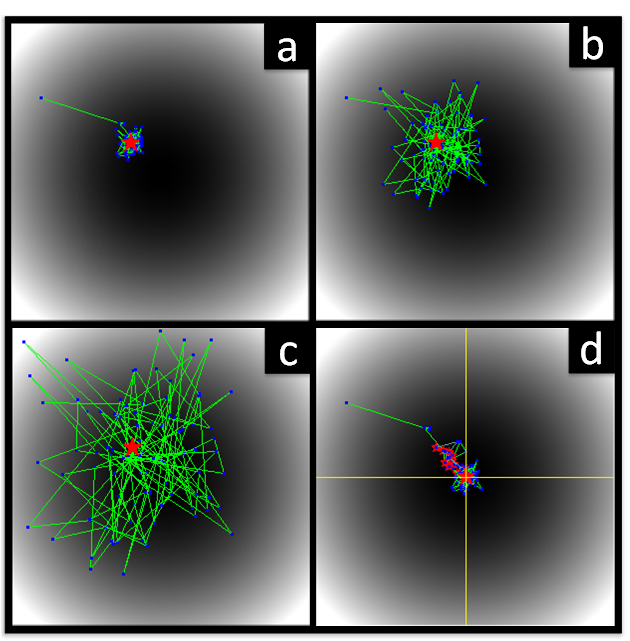
\includegraphics[scale=0.9]{Figuras/Movimento_Refinado.png}
	\caption{Testes com movimento refinado}
	\label{fig:Movimento_Refinado}
\end{figure}






\subsection{Visão imperial distorcida}

A movimentação de uma colônia em direção ao seu país imperialista nada mais é que a tendência da colônia  se parecer mais com seu império ao longo do passar de décadas. Para que a colônia se molde de forma a ter suas características mais parecidas com a de seu império, ela primeiro calcula o quão distante suas características estão do seu império, e então se movimenta em direção ao seu imperialista de acordo com um valor de assimilação. 

Quando uma colônia observa as características de seu império, para então calcular a distância entre cada característica, existe a possibilidade de que esta colônia não localize muito bem a posição ou valor exato da característica do seu império, de modo que tal distorção seja influenciada pelas posições das demais colônias do império. Assim, quando a colônia calcula o quão distante suas características estão de seu império, ela também observa quais são as características mais distantes ao imperialista, dentre todas as colônias, e adiciona um valor aleatório, distribuído normalmente, na característica do império, para então calcular uma distância com uma visão distorcida destas características do império.

  	Esta distorção é uma adição de ruído proporcional não ao espaço de busca em geral, mas sim em relação ao posicionamento de todas as colônias do império, isto é, em relação a área ou região do espaço de busca ocupada pelo império. Este tipo de ruído é uma otimização que faz com que a solução seja explorada localmente tal que a melhor solução seja encontrada mais devagar, porém explora localmente de forma aleatória o caminho a ser feito pela colônia, até que esta chegue ao país imperialista. Quanto mais próximas o grupo de colônias estiver de seu império, menor será a região ocupada pelo império e menor também será o ruído gerado. O ruído se torna nulo quando as colônias compartilharem as mesmas posições com seu império. Para se conhecer esta região do império, basta obter as distâncias máximas entre as colônias e o império, isto é, obtém-se os limites do império através das características mais distantes das colônias. Estes valores são armazenados localmente em um vetor \(maxDists\), que é gerado segundo o Algoritmo \ref{alg:CalculoMaxDists}
    
\vspace{10px}
\begin{algorithm}[h]
\SetAlgoLined
\KwData{
\\ Império - o império em questão.
\\ Colônias - o vetor de colônias.
\\ Dimensions - o valor que representa a quantidade de dimensões do problema.}
\KwResult{ 
\\maxDist - o vetor de distâncias máximas de cada atributo entre o império e todas as suas colônias.
}
maxDist = new Double[Dimensions]\;

\For{$i \leftarrow $0 \KwTo $Dimensions$}
{
	\For{$j \leftarrow $0 \KwTo $Império.NumColônias$}
    {
    	localDist = ABS(Império.Attributes[i] - Colônias[j].Attributes[i])\;
        maxDists[i] = MAX(localDist, MaxDist[i])\;
    }
}
\caption{ Cálculo das distâncias máximas para Visão Imperial Distorcida.}
\label{alg:CalculoMaxDists}
\end{algorithm}

Assim utiliza-se o vetor \(maxDists\) multiplicado de um valor aleatório distribuído normalmente e soma-o na posição do império, e então subtrai-se o valor da posição da colônia, para se obter o valor de distância distorcido, como mostra a equação \ref{eq:CalcVIDDist}:

\begin{equation}
\label{eq:CalcVIDDist}
\begin{split}
dist = 
&(Império.Attributes[i] + GausRand() \cdot maxDists[i]) - \\ &Colônia.Attributes[i]
\end{split}
\end{equation}

Após o cálculo da distância distorcida, o algoritmo da movimentação prossegue normalmente no seu fluxo como algo semelhante ao fluxo apresentado pela figura \ref{fig:Movimento_Original}, que será então multiplicada pelo coeficiente de assimilação e atribuída ao valor do atributo (ou característica), com a exceção de que agora não se calcula e nem se adiciona o ruído provido pelo valor aleatório baseado em \(\gamma\). 

Este método de adição de ruído é proporcional a distância entre a colônia e império, isto quer dizer que apenas quando o módulo da distância entre ambos for maior que zero é que existirá ruído. Assim quando a colônia se posicionar junto de seu império, não existirá alteração nenhuma na posição da colônia durante a etapa de movimento provinda do ruído. Ao comparar apenas uma colônia com um império, pode-se obter resultados que não sejam ótimos, porém esta alteração funciona muito bem com impérios que possuem várias colônias, uma vez que com muitas colônias tem-se uma exploração maior da região e a tendência será a de tornar o país menos custoso como sendo o centro do império utilizando a operação de possessão imperial.


A Figura\ref{fig:Testes_Vis_o_Imperial_Distorcida} mostra em \(a\) o caso de um país imperialista e uma colônia, com a operação de possessão imperial desativada. Observa-se que quanto mais próxima a colônia está do império, menos desvio ocorre em seu movimento. Em \(b\) tem-se o mesmo caso de \(a\) porém com a competição imperialista habilitada. Neste caso, existem algumas trocas entre império e colônia, porém a conversão para a melhor posição não ocorre. O item \(c\) representa uma configuração diferente, com 1 império e 9 colônias, totalizando 10 países, assim percebe-se como este tipo de movimento é sempre direcionado para o império, e ainda possui uma variação no movimento que decai junto a medida que a colônia chega perto do império. Por fim \(d\) é uma combinação de imagens que representam o cenário do item \(c\) durante as décadas de 1 a 5.

\begin{figure}[h]
	\centering
	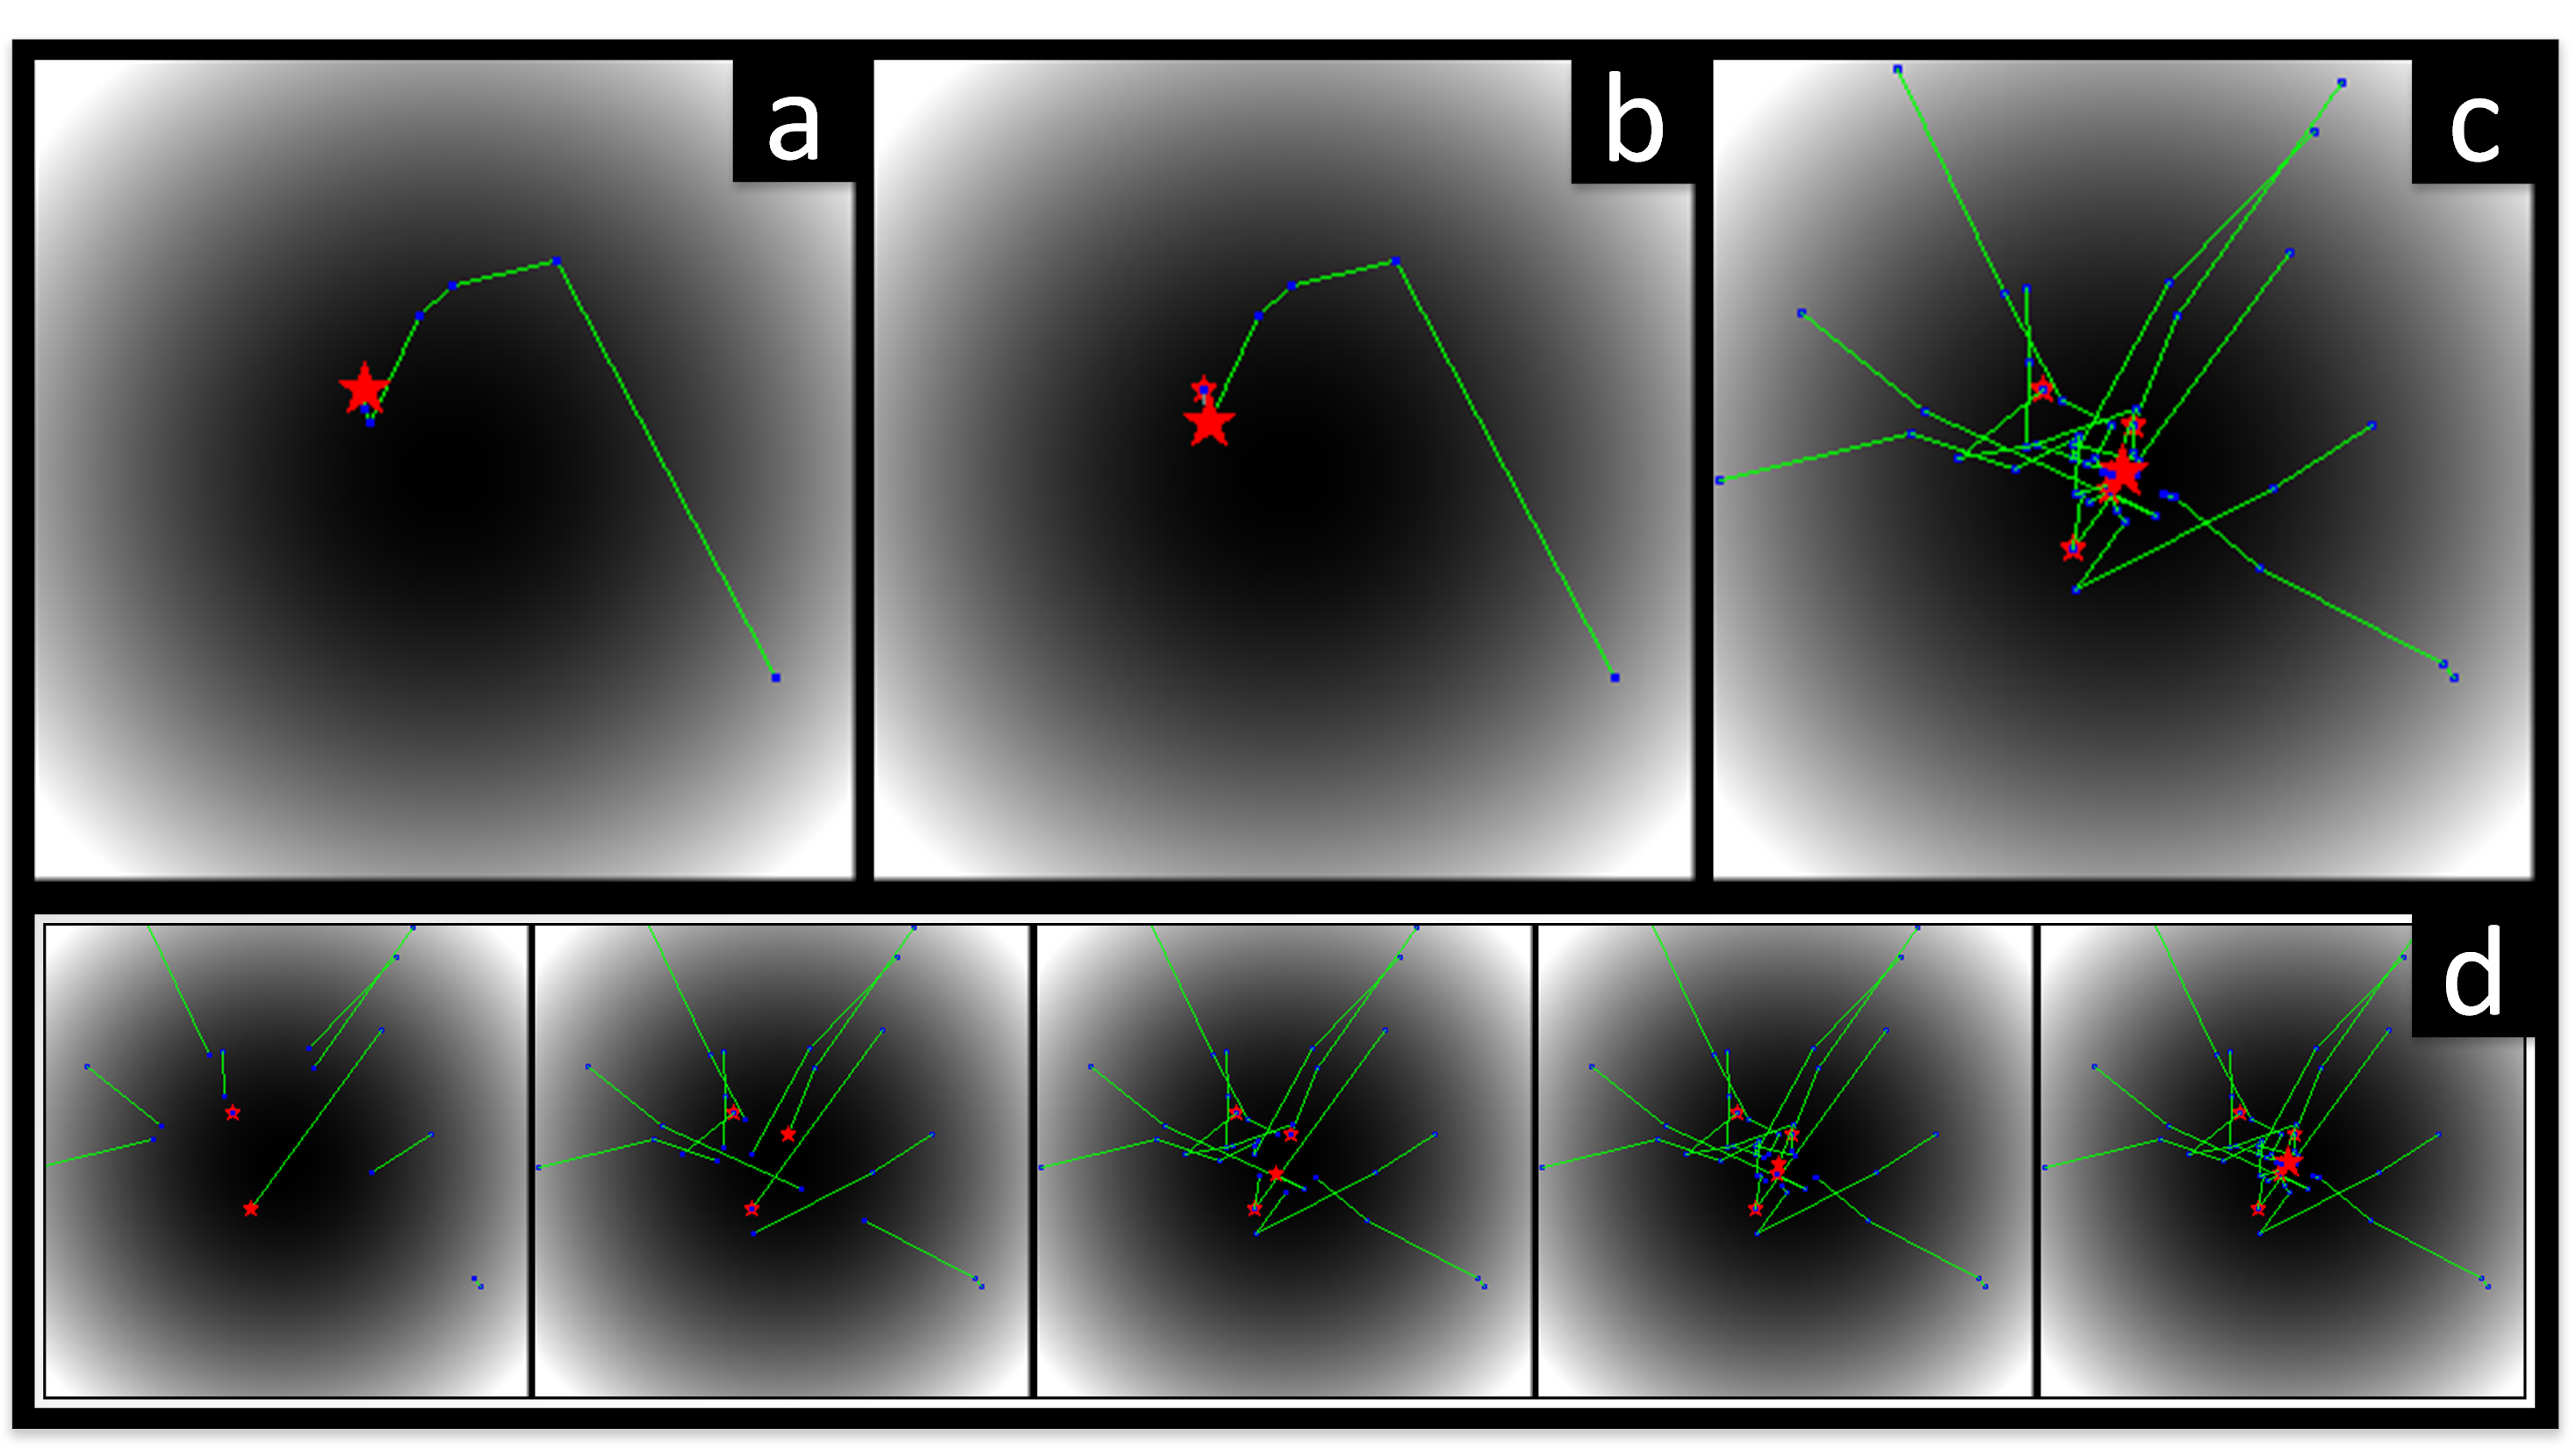
\includegraphics[scale=0.6]{Figuras/Testes_Vis_o_Imperial_Distorcida.png}
	\caption{Testes Visão Imperial Distorcida}
	\label{fig:Testes_Vis_o_Imperial_Distorcida}
\end{figure}

Comparando então ambas as alterações, com o método refinado de movimentação é possível controlar o ruído proporcionalmente ao espaço de busca, mesmo que suas dimensões estejam limitadas em valores e escalas completamente diferentes, possibilitando que um país tenha seu vetor de atributos composto por muitos mais elementos sem que o ruído seja um fator que atrapalhe a evolução da solução. Um ponto interessante para se analisar é a quantidade de ruído em relação a precisão da busca pela solução, de modo que tem-se como objetivo principal da movimentação, apenas a transição das características de um indivíduo até as características seu império, pois o algoritmo possui outros recursos, como o aumento do número de países e impérios, operação de revolução imperialista, e até mesmo a competição imperialista em si, fazem com que a adição de ruído pareça redundante. Porém, este não é o caso, o ruído quando usado em uma porcentagem baixa e durante a movimentação, melhora a busca pela melhor solução localmente, fazendo com que o império se mova para o vale (ou pico) local mais rapidamente (a movimentação de um império ocorre quando há troca a troca entre império e colônia, através da operação de possessão imperial). E por fim, como mencionado anteriormente, os demais métodos tem o objetivo de evitar que a solução fique estagnada em mínimos (ou máximos) locais, uma vez que possuem apenas o fator aleatório e não são direcionadas, como a movimentação. 

Já o método de movimentação por visão imperial distorcida tem como intuito apenas inserir ruído que seja proporcional às colônias mais distantes do império, trazendo a ideia de que quanto mais distante uma colônia está de seu império mais míope ela é para definir as características de seu império. Assim a exploração do espaço de busca não formará caminhos em linha reta, mas sim caminhos que sejam aleatórios até que a colônia de fato chegue ao império. Esta forma aleatória de se mover pode aumentar o tempo que uma colônia leva para chegar até seu imperialista e lá ficar estagnada, mas por outro lado aumenta a chance do império sair de mínimos (máximos) locais se deslocando pelas décadas através da operação de possessão imperial.

Ambos os métodos ainda possuem um mecanismo de ‘freio’, geralmente relativo ao número máximo de décadas, usado para decrementar gradualmente a quantidade de ruído gerada durante as décadas até que esta quantidade de ruído seja anulada ou se mantenha fixa em um valor. Assim como o decrescimento da operação de revolução colonial decresce, a quantidade de ruído também decresce, porém existe a possibilidade de manter este ruído até o fim (até que uma condição de parada seja atingida), ou também existe a possibilidade de controlar o decrescimento para que os ruídos sejam decrementados até se anularem durante o processo evolutivo. Quando os ruídos tendem a se anular, a forma de movimento tende ao método de movimento linear, que por sua vez é mais rápido e leva à conversão ideal (onde os países estejam na mesma posição de seu imperialista). Desta forma, pode-se ter uma quantidade grande de ruído nas primeiras décadas, de modo a explorar melhor o espaço de busca, evitando mínimos locais, e gradualmente diminuir o ruído para ajustar a posição do império para a melhor possível e por fim, anular os ruídos para que o processo evolutivo possa convergir para o cenário ideal.

A combinação de ambos os métodos mantém a velocidade de deslocamento do império durante as décadas constante, porém mantém o ruído gerado pela visão imperial distorcida sempre ativo nas colônias que sofreram deslocamento por ruído refinado na década passada, isto é, o ruído gerado pelo método refinado faz com que algumas colônias sempre estejam fora do centro do império e limitados em uma região proporcional ao espaço de busca, então, na próxima década, será aplicado a elas, o ruído gerado pela visão imperial distorcida (pois ele é usado quando se calcula a distância, antes de se aplicar o ruído gerado pelo método de movimento refinado), assim este ruído gerado pela visão imperial distorcida será constante e limitado no espaço definido pelo método de movimento refinado, e como ele é proporcional distância entre colônia e império, também passa a ser proporcional ao limite definido no ruído gerado no movimento refinado. A figura\ref{fig:MovimentoCombinado} mostra a evolução durante as décadas 1, 4 e 8 respectivamente nos itens \(a\), \(b\) e \(c\).

\begin{figure}[h]
	\centering
	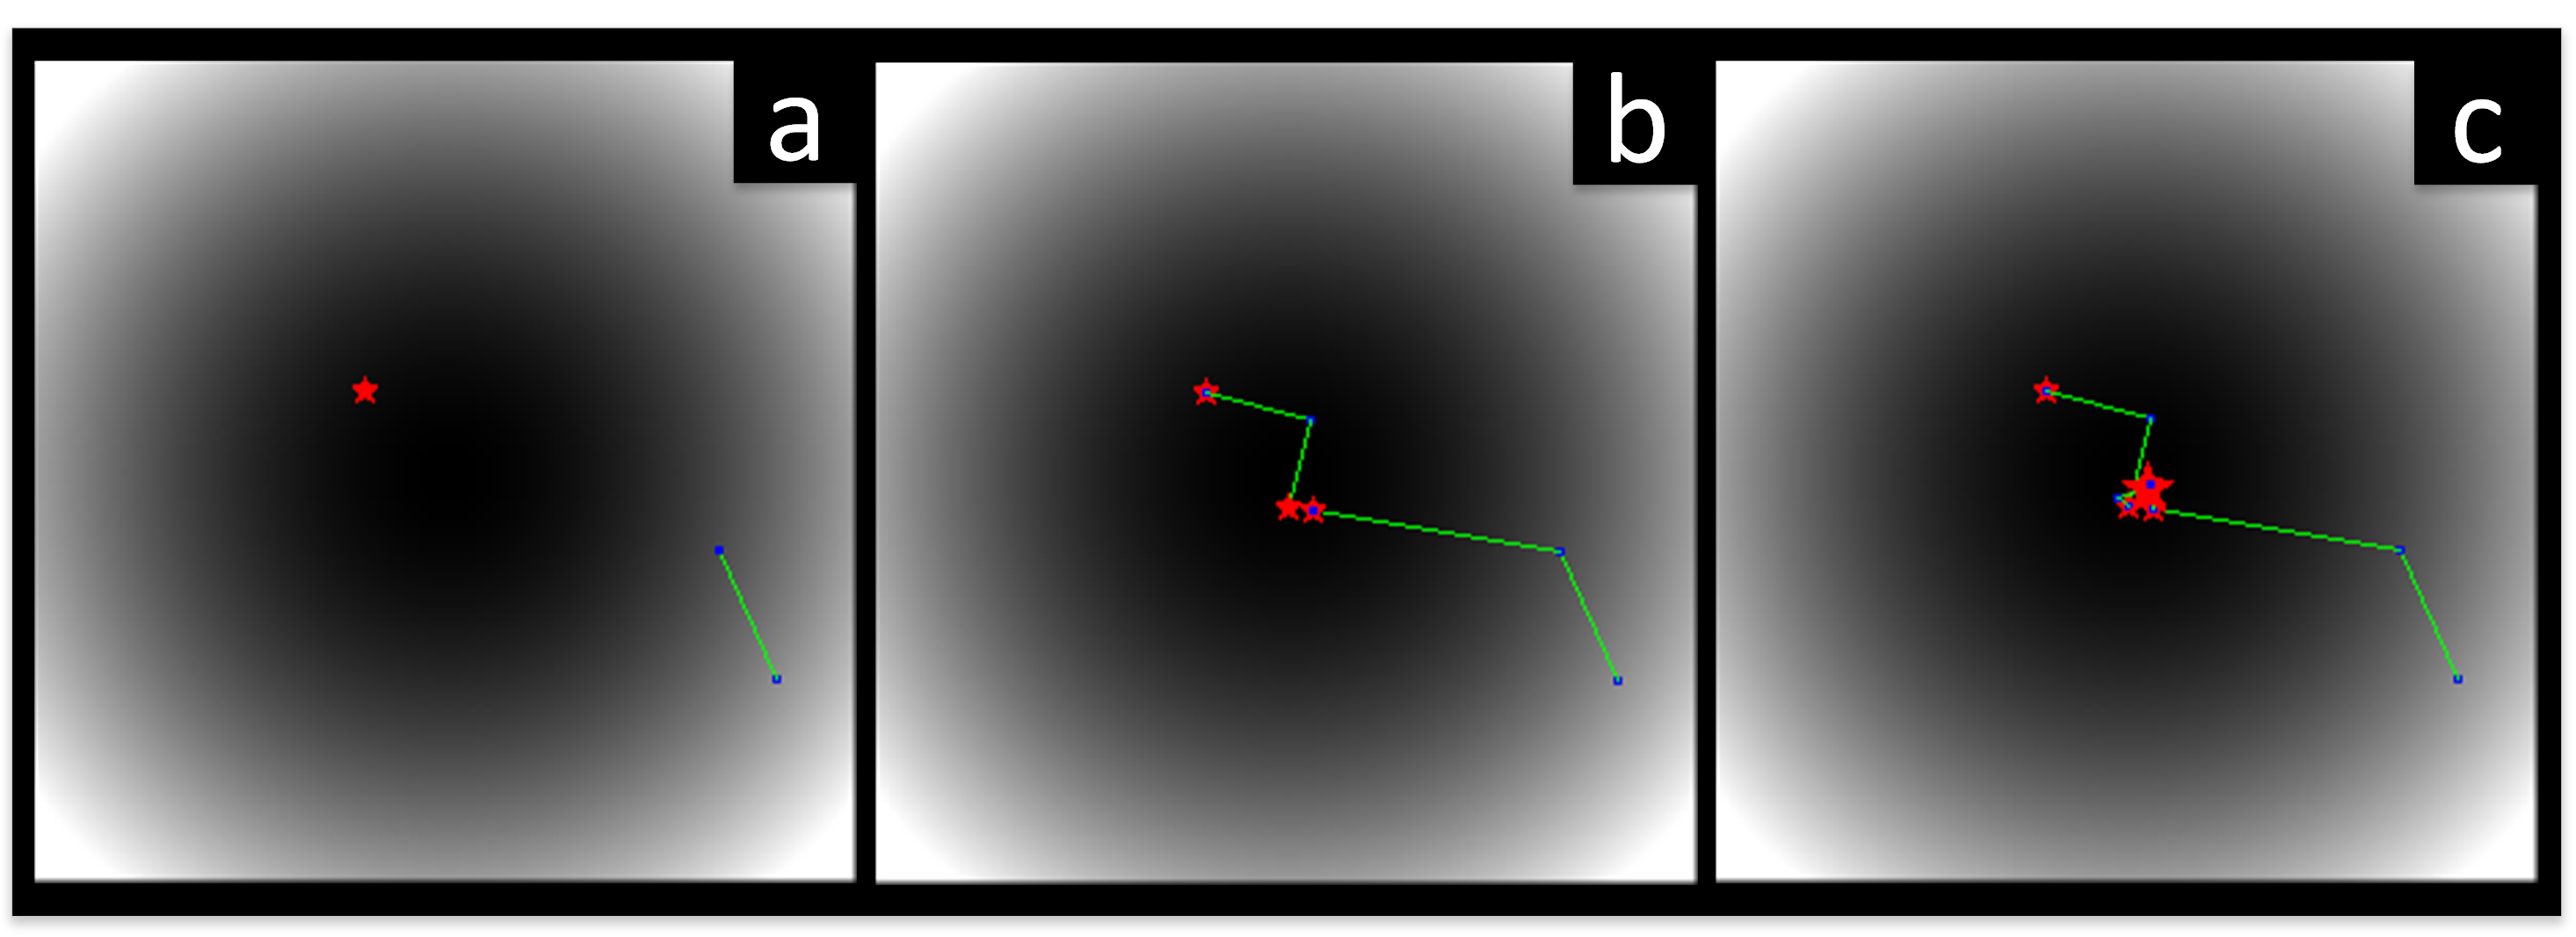
\includegraphics[scale=0.6]{Figuras/MovimentoCombinado.png}
	\caption{Movimento combinado}	
    \label{fig:MovimentoCombinado}
\end{figure}

Concluindo esta seção, tem-se agora três (Refinado, Visão imperial distorcida e Combinado) métodos capazes de mover os países, inserindo ruídos proporcionais ao espaço de busca de forma controlada e que ainda é capaz de atingir o cenário ideal de convergência, diferentemente do modelo proposto por \citeauthor{atashpaz2007imperialist} em \cite{atashpaz2007imperialist} e \citeauthor{roche2011imperialist} em \cite{roche2011imperialist}, ao adicionar o ruído fixo, o qual levaria a impossibilidade de convergência para o cenário ideal. O método combinado pode apresentar soluções melhores, mas em contrapartida são necessários mais cálculos e consequentemente mais processamento. Caso a função de aptidão(\emph{Fitness}) seja de rápida avaliação, é ideal usar o modelo refinado, para ruídos independentes da distância entre colônia e império, ou o método de visão distorcida, para ruídos dependentes da distância. já em casos onde o problema apresenta alto custo computacional, o cálculo da forma de movimento não será tão impactante, porém aconselha-se fazer com que os ruídos cessem após uma quantidade de décadas para que a solução possa convergir para o cenário ideal, encontrando o ponto ótimo entre o quanto se deve explorar o espaço de busca de forma mais aleatória e o quão rápido se deve convergir. 






\section{Paralelização do ICA}

Algoritmos evolutivos têm como parte essencial para convergência a função de aptidão, que deve ser bem definida e voltada para o problema. Tal função, deve ser executada durante todas as décadas. No ICA, a função de aptidão proposta foi definida de forma a executar cálculos os quais resultam em um valor de custo para o país, tal que este custo seja utilizado por todos os componentes do ICA, a fim de buscar pela melhor solução. A quantidade de chamadas à função de aptidão é dependente basicamente de dois valores, do número de países \(np\) e número de décadas \(nd\). 


Sabendo que os países sempre são avaliados, todos de uma só vez, e que em cada década todos os países devem ter seu valor de custo calculado, pode-se dizer que em cada década seus atributos se modificam de acordo com a posição de seus impérios. E ainda, leva-se em conta que inicialmente todos os países são avaliados e têm seus custos atribuídos, antes mesmo da separação entre colônias e impérios. Desta forma, é possível calcular a quantidade total de chamadas da função de aptidão durante uma execução completa do ICA como sendo:


\[np x (nd + 1)\]


Dependendo do tipo de problema, algoritmos evolutivos podem levar diversas épocas, no caso do ICA, décadas, para convergir em uma solução dentro dos critérios de parada (que foram definidas no capítulo x). Em casos cujo problema se expande para o domínio não linear existe a possibilidade de executar tais operações muito mais vezes do que o esperado para se chegar ao resultado. 


No problema a ser solucionado por este trabalho, a função de aptidão utilizará muito processamento para o cálculo de custo de cada país. Para que tal solução possa ser executada diversas vezes, em tempo hábil, e também de forma que o problema possa ser testado dentro de diferentes abordagens, é necessário utilizar todos os recursos tecnológicos disponíveis. 


Para otimizar a velocidade com que o ICA faça tais cálculos, foi desenvolvida uma adaptação na parte central do ICA, de forma que as chamadas para avaliação das funções de custo dos países sejam executadas paralelamente, já que o cálculo de custo do país são independentes dos demais indivíduos, usando todos os núcleos de processamento possíveis. Assim, a aplicação tem um ganho significativo de tempo e um aumento significativo de processamento, que depende de quantos núcleos estão disponíveis para a execução do ICA


Um fato técnico interessante, é que para se utilizar de forma ótima toda esta alocação de núcleos de processamento, devemos levar em conta que o número de indivíduos deve ser múltiplo do número de núcleos de processamento para que todos sejam utilizados com capacidade máxima para o processamento da função de aptidão. Caso este número seja diferente, também haverá uma melhora, porém um dos núcleos poderá ficar ocioso durante os cálculos, fazendo com que indiretamente se “perca” a capacidade total de processamento em um ou mais núcleos. 


A paralelização dos cálculos de custos dos países foi implementada de modo a ser opcional. Por padrão já está ativa, porém ao se configurar os dados iniciais para a solução de um dado problema, fica a critério do desenvolvedor, decidir se utilizará ou não o algoritmo de forma paralelizada.


Algo que pode ser chamado de desvantagem em se paralelizar esta parte do algoritmo, aplica-se apenas no momento em que é necessário executar uma depuração no código que faz o cálculo do custo do país. O que ocorre no caso normal, não paralelo, é que para se depurar uma função, se escolhe uma parte do código, a qual se deseja depurar e então a execução do programa sofrerá uma pausa quando chegar naquele ponto. Quando se utiliza a técnica de paralelização para executar as funções (neste caso as funções são as mesmas, porém apenas a chamada da função é alterada), cada núcleo disponível irá alocar uma tarefa (thread) para executar as funções em paralelo, assim, como foi definido um ponto de depuração dentro da função, toda vez que uma das tarefas atingir o ponto de depuração, ela irá pausar a execução do programa, apresentando os valores a serem depurados para o seu contexto de execução da tarefa, e impedindo que uma depuração por passos possa ser feita sequencialmente apenas em uma tarefa sem que um filtro seja criado em tempo de execução. Tal filtro de depuração para pontos de parada só podem ser adicionados em tempo de execução porque inicialmente não se sabe qual será a identificação da tarefa que irá rodar em paralelo por ela não ter sido criada ainda. É importante fixar que a depuração não é impedida ou resulta em erros, mas tal desvantagem se dá na adição de passos para filtrar e isolar a depuração para apenas uma tarefa.


A melhora no desempenho não é apenas dependente da paralelização do cálculo dos custos dos países, mas também, do que está dentro do algoritmo que faz o cálculo e também da configuração e estado da máquina que executará o processamento. é muito importante que se tome cuidado durante o desenvolvimento para que a função de avaliação, quando processada em paralelo, não compartilhe recursos entre as tarefas, pois isto pode causar a execução em serial, já que o algoritmo de paralelização ‘trava’ o uso de um recurso apenas para uma tarefa. Outro problema que ocorre com o compartilhamento de recursos é a inconsistência, pois caso haja escrita, uma tarefa pode alterar um recurso que será usado por outra tarefa. Como a função de aptidão do ICA é uma implementação da interface IFitness, estes tópicos devem ser tratados com cuidado durante o desenvolvimento do problema para que a paralelização funcione de forma ótima.




\section{Formulação do ambiente}

Os dados de entrada iniciais utilizados para o desenvolvimento da solução representam e classificam, quando e onde ocorreram instalações na rede de distribuição elétrica de uma dada região. O objetivo é obter a partir destes dados a previsão de expansão espacial urbana, no caso, relativo à densidade de carga elétrica. Assim pode-se aplicar tal previsão no planejamento de cargas, em sistemas inteligentes de energia (smartgrids), gerenciamento de cargas (reposicionamento de transformadores ou subestações para localizações mais apropriadas), dentre outros. 

Para o desenvolvimento da metodologia de previsão de densidade espacial urbana é necessária a análise de fatores que caracterizam um ou mais fatores de representação para densidade (estes são fatores que variam no tempo), e de fatores que representam o espaço em que estes fatores de densidade se aplicam. Isto quer dizer que, inicialmente, é necessário o uso de dados concretos baseados diretamente na posição geográfica em que o fator de densidade se encontra e evolui durante o tempo, de modo que a posição geográfica do fator represente, de fato, um ponto no espaço ao qual será prevista a evolução dos fatores de densidade durante um determinado intervalo de tempo.

Entende-se como fatores que representam o espaço em que os fatores de densidade evoluem, como sendo uma composição de fatores que possuem relação direta com o fator de densidade, de forma a representarem este fator de dentro de um plano espacial, que neste caso, são utilizados os pontos de latitude e longitude citados acima para representar a existência deste determinado fator (neste caso, a instalação de ponto da rede elétrica propriamente dita) dentro do espaço em questão. Então tem-se um espaço bidimensional formado por pontos de latitude (representado pelo eixo das ordenadas) e longitude (representado pelo eixo das abcissas), e limitado em latitudes e longitudes, máximas e mínimas, formando uma região retangular que contém tal representação dos fatores de densidade.

Ainda sem se preocupar com os fatores de densidade que se alteram durante o tempo, apenas focando nas posições geográficas que compõem os dados, faz-se o uso da filosofia de quadriculas \cite{willis2002spatial}, para tornar o espaço homogêneo, pois inicialmente, este espaço era representado por um conjunto de pontos espaçados desigualmente, de modo que seria muito custoso computacionalmente representar e processar todos os dados de forma a cumprir o objetivo apresentado por este trabalho.

Assim, é possível gerar um mapa de quadrículas homogêneas que representará os dados iniciais na forma de uma matriz, com a altura (número de linhas) sendo o número de quadrículas de norte a sul, e largura (número de colunas) como sendo o número de quadrículas de leste a oeste. Tal matriz pode ser usada para mapear uma região geográfica em uma matriz de dados que possa ser computada sem que seja preciso se preocupar com os fatores de localização geográfica, como por exemplo, converter ou calcular a distância entre 2 pontos geográficos, pois o espaço entre as quadrículas já é normalizado.

Para se fazer previsão de densidade espacial urbana é necessário que se modele um cenário no ambiente computacional, que seja capaz de representar com um certo nível de fidelidade, o que o ambiente real representa. Para criar tal ambiente computacional é preciso primeiro a geração ou obtenção de uma quantidade de dados os quais serão usados na modelagem deste ambiente. Os dados em questão referem-se a densidade de cargas, que é analisado em uma região urbana de forma espacial. 

A base de dados utilizada para fazer a previsão de densidade de carga espacial urbana representa uma estimativa das datas de instalação de pontos de rede elétrica  durante um período de tempo e de uma determinada região e, portanto são dados que variam no tempo. Os pontos de instalação elétrica foram classificados em residencial, residencial de baixa renda, comercial, industrial, público e rural. Inicialmente imaginou-se que pontes, ruas, rios, altitude, inclinação, etc. poderiam ser úteis como dados de atração, representando pontos que não variam em pequenos intervalos de tempo, e portanto, fixos durante todos os períodos, porém foram removidos para que a análise ficasse mais limpa, pois estavam gerando ruído nos resultados e acumulando muito erro durante a previsão. Então, cada ponto de instalação elétrica possui um município, um grupo, uma data de criação e valores que definem sua localização geográfica, representados por valores numéricos reais de latitude e longitude. Com estes dados separados é possível então criar um banco de dados para armazenar toda informação que é captada, gerada ou obtida, normalizando assim toda entrada de dados para a aplicação apenas nestas 5 características.

Com a tabela possuindo um número grande de dados durante os períodos, é possível separar estes dados em diversos mapas matrizes (mapas de quadrículas) representando a quantidade de carga instalada em cada região e sua evolução durante um período de tempo. A quantidade de mapas é definida pelo intervalo de tempo que se deseja processar. Por exemplo, se inicialmente foram obtidos dados nos períodos entre 2005 até 2015, e o período de tempo desejado é de um ano, geram-se então, 10 mapas matrizes de densidades de carga onde cada mapa matriz possui a densidade de carga para cada período, neste caso, para cada ano.

Antes de gerar os mapas matrizes, ainda é necessário mais um passo, que é a criação de arquivos, a partir do banco de dados, onde cada arquivo representa o período em que se deseja obter os mapas matrizes. Para isto, foram criados diversos filtros no banco de dados para cada período, onde cada filtro seleciona todas as linhas que estejam dentro do intervalo de duas datas, uma inicial e outra final, sendo que destas duas datas, a data inicial é referente sempre a data do período inicial, e a segunda é referente ao período em questão, pois os dados devem representar valores crescentes, e não a diferença entre os períodos. Outra funcionalidade que cada filtro aplica nas linhas, é a adição de um valor de contagem, denominado “Total”, para cada ponto de coordenada geográfica que possa ter sofrido crescimento, sendo este aumento referente a mais instalações de pontos de rede elétrica nesta mesma coordenada, como por exemplo a construção de um prédio, residência ou qualquer outro tipo de adição que possa vir a representar uma forma de crescimento de consumo de carga para aquela coordenada. Assim, cada arquivo deve ser salvo em modo texto, possuindo os nomes seguindo a seguinte forma, \(“<período0>.csv”, “<período1>.csv”, ..., “<períodoN>.csv”\), e ainda dentro dos arquivos, os dados serão filtrados de modo que transformem a tabela inicial em uma tabela contendo os campos: Longitude, Latitude, Grupo e Total.

Toda a modelagem dos dados de carga citados anteriormente ocorreram fora da aplicação, e foi utilizada a ferramenta \(sqlite\) para a criação, armazenamento e filtragem dos dados para a utilização destes na aplicação. Já na aplicação, a primeira definição que deve ser feita é sobre a região que se deseja utilizar, sendo esta definida por valores de longitude, leste e oeste, e valores de latitude, norte e sul. Com estes quatro valores formando um setor terrestre quadrangular, onde tal setor representa a região que se deseja processar para obter a previsão espacial de carga. Os dados presentes nos arquivos gerados para cada período que estiverem fora destes intervalos de (norte, sul e leste, oeste) serão ignorados, sendo apenas processados os dados dentro dos intervalos citados. 

Os valores presentes nos arquivos de período ainda não estão discretizados, de forma que possam ser processados de forma mais homogênea, então, para utiliza-se a técnica de quadriculamento do setor para discretizar as regiões de forma a fazer com que o mapa seja particionado em tamanhos iguais e, consequentemente cada parte igual do mapa receba um valor de carga de acordo com aquela região. Assim, forma-se um mapa, denominado \(Mapa Matriz\), para cada período, que representa a densidade de carga espacial em porções homogêneas.

A segunda definição deve ser o tamanho de cada quadrícula, que é definida a partir de apenas um valor numérico, que representa o tamanho dos seus lados em metros. Com estas duas definições iniciais pode-se então criar um mapa de quadrículas que será usado posteriormente como base para a geração dos mapas matrizes. 
	
O mapa de quadrículas utiliza-se destes 5 valores iniciais para ser gerado, e nele definem-se as quantidades de quadrículas que irão compor o mapa em altura e largura, e consequentemente a quantidade de quadrículas total do mapa, que pode ser calculado multiplicando a altura com a largura. Os valores de altura e largura são calculados em duas etapas, onde a primeira etapa fornece a largura/altura total em metros e a segunda etapa resolve a quantidade de quadrículas para altura e largura, dividindo os valores de altura e largura totais em metros pelo tamanho de cada quadrícula em metros, como pode ser visto nas equações \ref{eq:building-matrix-map-one} e \ref{eq:building-matrix-map-two}:

\begin{equation}
\label{eq:building-matrix-map-one}
\begin{split}
widthInMeter = Abs(DistanceTo(north, east, north, west));\\
heightInMeter = Abs(DistanceTo(north, east, south, east));
\end{split}
\end{equation}

\begin{equation}
\label{eq:building-matrix-map-two}
\begin{split}
mapWidth = widthInMeter / quadricSizeInMeter;\\
mapHeight = heightInMeter / quadricSizeInMeter;
\end{split}
\end{equation}

A chamada função \(DistanceTo\) calcula a distância em metros entre dois pontos de coordenadas geográficas quaisquer utilizando a fórmula de haversine \cite{shumaker1984astronomical}, \cite{snyder1987map}, onde os dois primeiros valores representam o primeiro ponto e coordenada geográfica e os últimos dois valores representam o segundo ponto de coordenada geográfica. Observa-se que na primeira chamada, mantiveram-se os pontos de latitude fixos em norte, de forma a deslocar-se apenas horizontalmente (de leste para oeste) e na segunda chamada mantiveram-se fixos os pontos de longitude fixos em leste, de forma a deslocar-se apenas verticalmente (de norte para sul), para assim obter o valor transformado de coordenada geográfica para coordenada cartesiana em metros, para largura e altura respectivamente.

Com a quantidade de quadrículas para altura e largura calculados para o mapa de quadrículas, agora é preciso popular cada índice do mapa com uma quadrícula. Cada quadrícula é representada por um ponto de coordenada geográfica, composto por latitude e longitude, podendo este ser convertido em uma distância a partir do ponto inicial ou em um ponto de utm (que é o ponto de coordenada geográfica representado pela \emph{Universal Transversa de Mercator}). Então, para isto, são necessárias mais duas definições, um ponto inicial e uma direção de iteração. 

O ponto inicial pode ser definido como qualquer combinação dos valores de latitude e longitude dados inicialmente, então, pode-se ter o ponto inicial como sendo\( (Norte, Leste)\), \((Norte, Oeste)\), \((Sul, Leste)\) ou \((Sul, Oeste)\), porém deve-se prestar atenção em definir a direção como sendo a oposta ao ponto inicial, uma vez que o processo de inicialização do mapa de quadrículas já possui seus limites definidos e a direção é quem define para qual sentido serão geradas as quadrículas (iterando-se em altura e largura) a partir do ponto inicial. Então, por exemplo, se o ponto inicial for \((Norte, Leste)\), a direção de crescimento deve ser representada pelo texto \(“so”\), assim, tem-se uma iteração que gera quadrículas dentro dos limites do mapa de quadrículas, que vai de Norte para Sul e de Leste para Oeste. Caso a direção de crescimento para o mesmo ponto do exemplo seja outra, digamos, \(“sl”\), o mapa terá como ponto inicial os pontos definidos como Norte e Leste, crescerá de norte a sul, porém de Leste a leste, tendo um deslocamento para fora dos limites do mapa de quadrículas esperado, o que pode implicar em um preenchimento incorreto do mapa matriz, que define as cargas, nos próximos passos da aplicação.
	
Finalizando a criação do mapa de quadrículas, ainda são definidos 5 valores e uma função, sendo estes, o Ponto Final, que representa o ponto mais distante ao ponto inicial, tendo sua distância como a diagonal principal do mapa de quadrículas, e os valores para Latitude Máxima, Longitude Máxima, Latitude Mínima, e Longitude Mínima, definidos a partir dos pontos inicial e final. Estes últimos 4 valores, são usados pela função a ser definida, que, por sua vez, calcula os índices \((x,y)\) do mapa de quadrículas, a partir de um ponto de coordenada geográfica (Latitude, Longitude), isto é, dado um ponto na forma (Latitude, Longitude), a função deve retornar em qual quadrícula do mapa de quadrículas (mapa matriz) este ponto se encontra. Esta é uma função usada para preencher os mapas matrizes a partir dos dados nos arquivos de períodos.

Com o mapa de quadrículas criado, inicializado e seus valores propriamente definidos dentro dos limites estipulados (Norte, Sul, Leste, Oeste), sua estrutura pode ser ilustrada como apresentada na figura \ref{fig:Ilustrations-QuadricMap}: 


\begin{figure}[h]
	\centering
	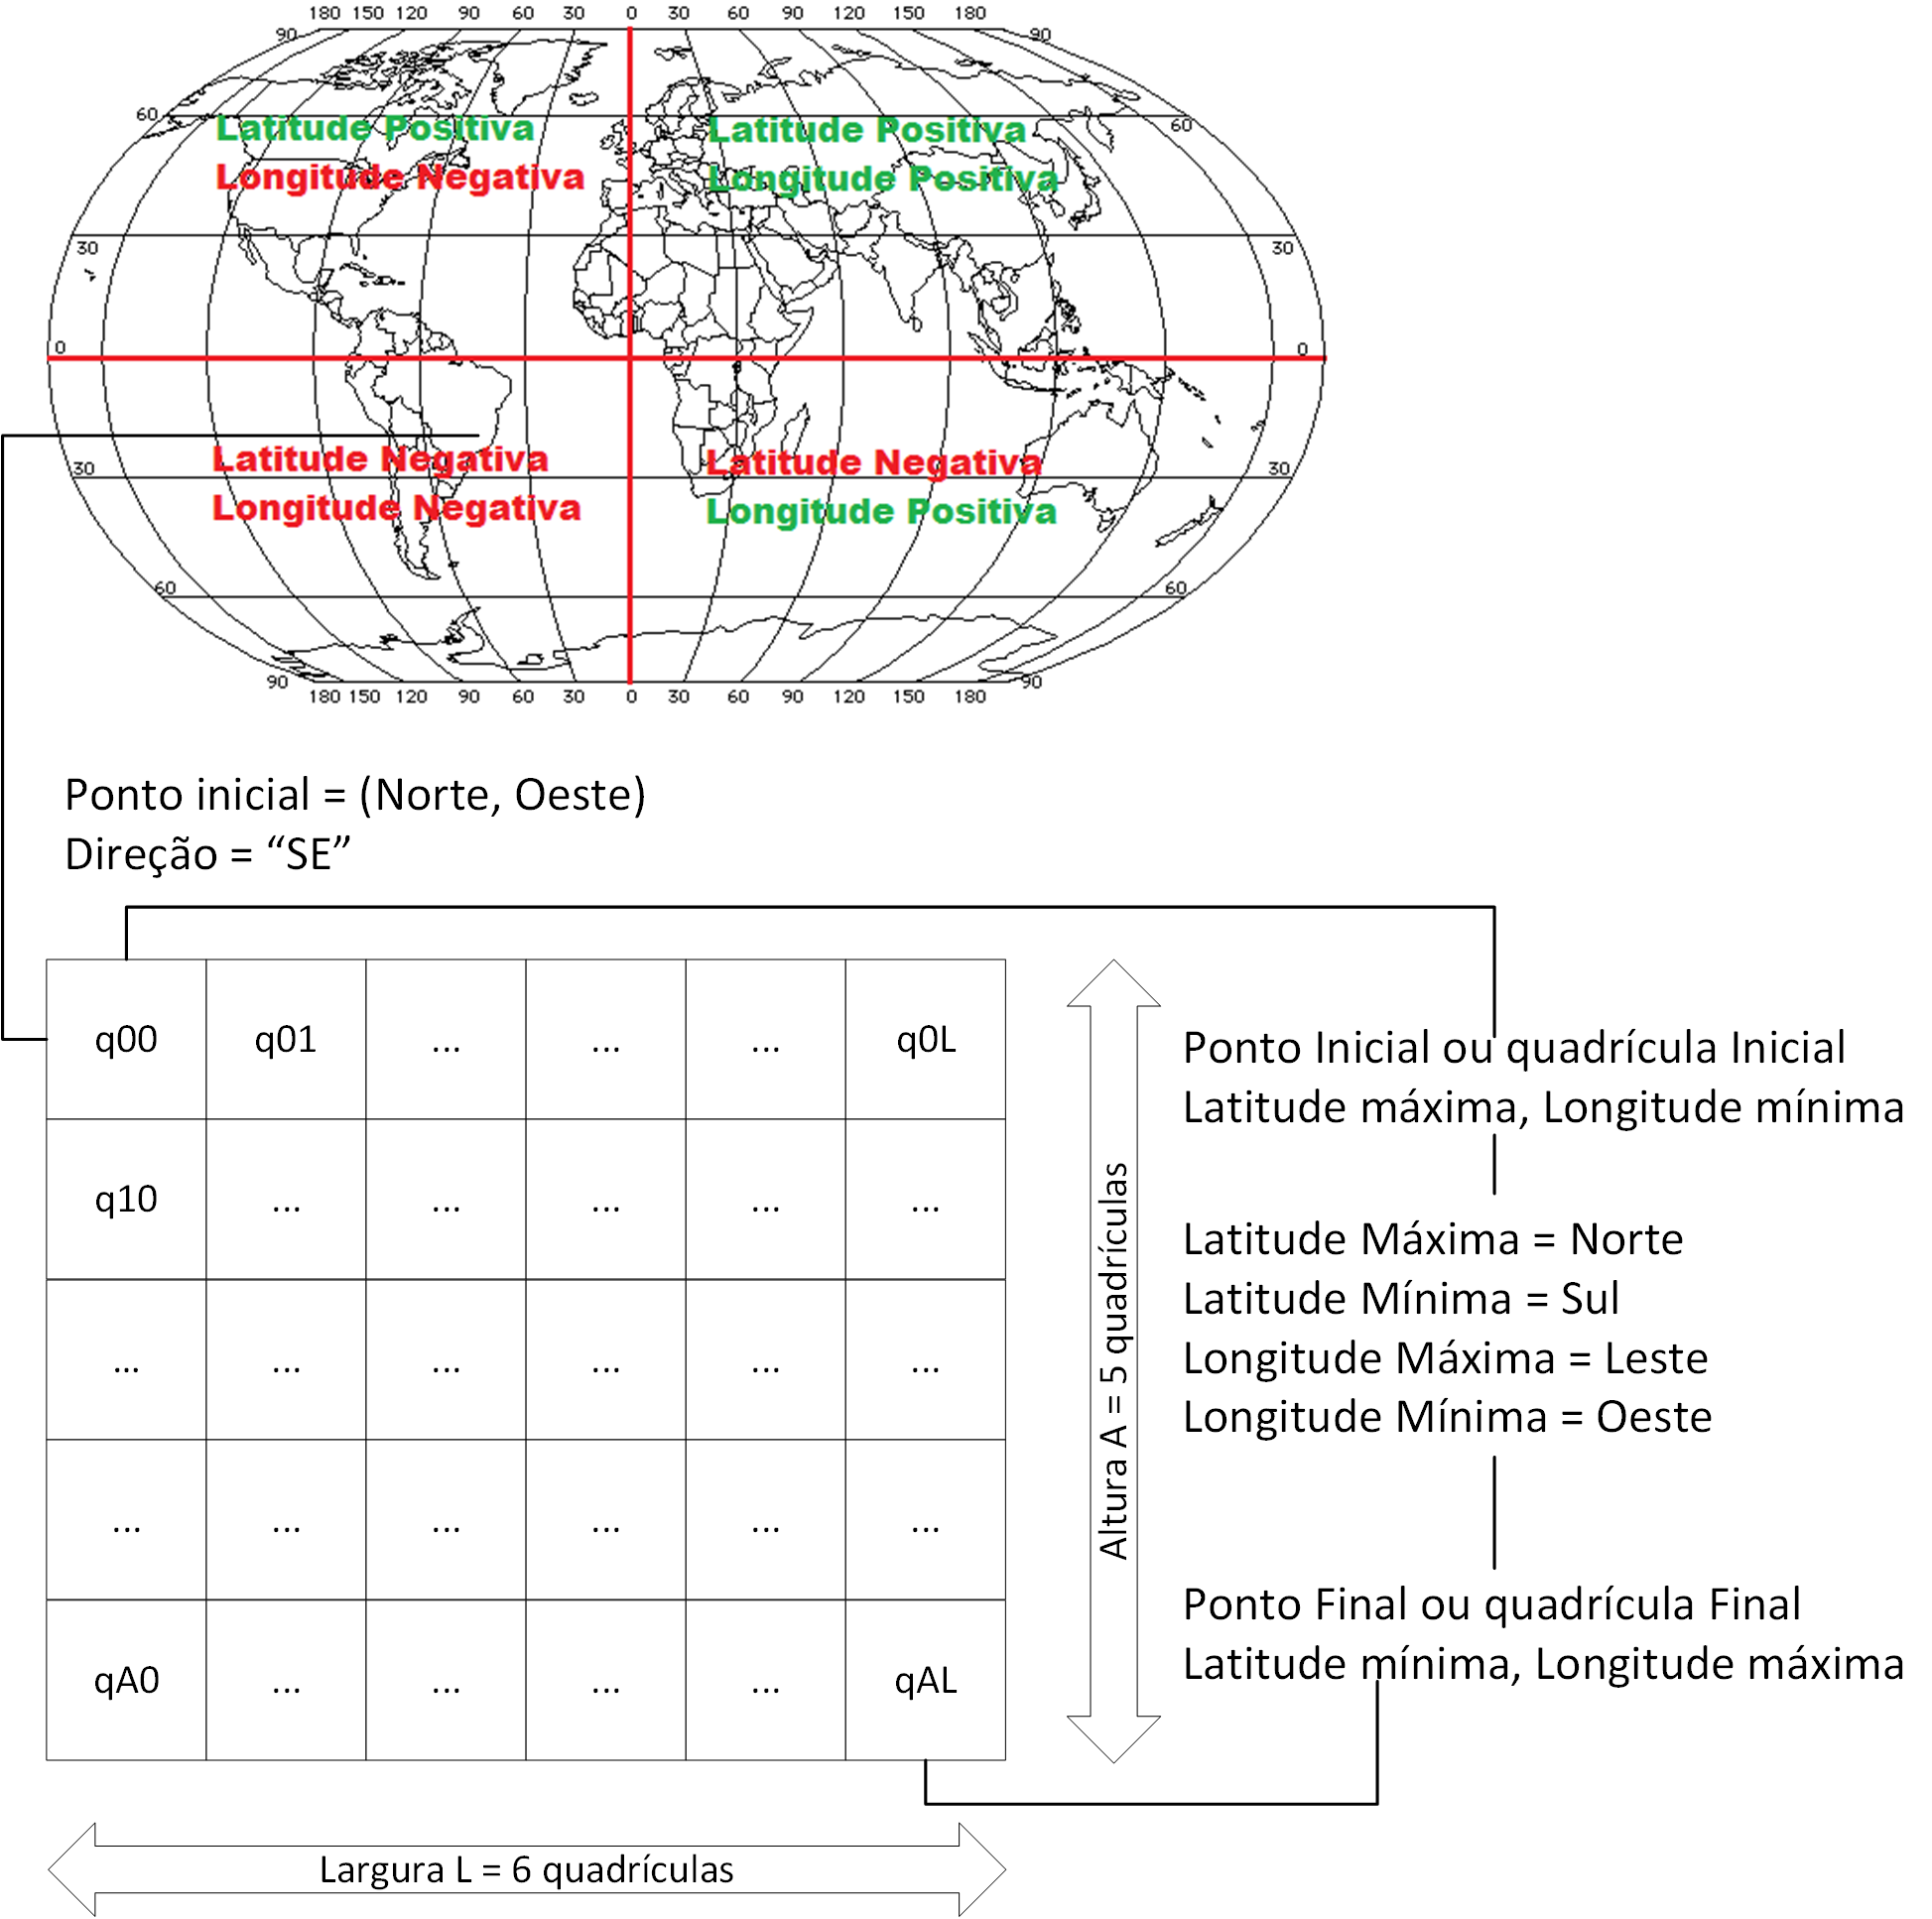
\includegraphics[scale=0.6]{Figuras/Ilustrations-QuadricMap.png}
	\caption{Ilustração da montagem do mapa de quadrículas.}
	\label{fig:Ilustrations-QuadricMap}
\end{figure}


Observe a região escolhida está no hemisfério sul a esquerda do meridiano de \emph{Greenwich}, o que indica que os valores para latitude e longitude (em graus) sempre serão negativos, e assim, de acordo com a posição inicial e a direção escolhida, os valores máximos para latitude e longitude se resolvem como apresentado.

Passando agora para os mapas matrizes, que nada mais são que uma lista de matrizes com o mesmo tamanho, em altura e largura, do mapa de quadrículas, e tal que a quantidade de mapas matrizes é referente a quantidade de períodos. Cada índice de um dado mapa matriz é diretamente mapeado para uma quadrícula do mapa de quadrículas, podendo assim, este mapa matriz representar um mapa de densidades genérico, sem relação direta ao mapa de quadrículas, porém pode-se usar o mapa de quadrículas para localizar e dar sentido ao mapa matriz sempre que necessário. 

Tal encapsulamento dos valores de densidade em uma lista de mapas matrizes, de tamanhos iguais, e de forma que seus índices representem valores de densidade, os quais são crescentes de acordo com o período de cada mapa matriz, faz com que a aplicação seja capaz de processar qualquer mapa de densidades sem se 'preocupar' com a localização geográfica real que este mapa matriz representa. O mapa de quadrículas então, tem duas funcionalidades básicas, que é a de inicializar a região a partir dos dados iniciais, e abstrair as informações geográficas para os mapas matrizes, os quais representam as densidades de carga em cada período.

A partir do mapa de quadrículas gerado e o conceito dos mapas matrizes, pode-se então, escolher qualquer fator para inserir em seus índices, como por exemplo, pode-se criar um mapa de quadrículas para uma determinada região tal que o fator escolhido sejam valores de altitude ou de inclinação. Porém para que uma previsão seja feita é necessário utilizar dados de densidade que variam de acordo com o tempo, como é o caso dos dados citados no início desta seção, os quais podem ser mapeados em vários mapas matrizes cada um representando um período de tempo diferente e diferenciados pelo mesmo intervalo de tempo, como por exemplo, poderia ser gerado um mapa de quadrículas do total de instalações elétricas até 2010, um até 2011 e assim por diante.

Sabe-se que os fatores de densidade devem estar diretamente relacionados com os valores de posição geográfica, por isto podem ser inseridos em qualquer mapa de matriz, e que também, devem variar no tempo, para que possam ser gerados diversos mapas de matrizes, com cada fator representando assim, um período de tempo bem definido e espaçados no tempo uniformemente, tal que possam ser geradas previsões futuras à estes períodos e de mesmo intervalo de tempo.

	Neste trabalho, ainda não foi modelada a previsão de múltiplos fatores, mas já foi elaborada uma estrutura que converge vários fatores de carga para apenas um fator de densidade de carga, denominado “multiplicadores de carga”.

Para a criação da lista de mapas matrizes, é então, utilizado o mapa de quadrículas já processado, os arquivos de períodos e uma estrutura que representa a densidade de carga de cada tipo de região, denominada “multiplicadores de carga”. Para este trabalho foram considerada as regiões do tipo residenciais (\(m=1\)), comerciais (\(m=3)\), industriais (\(m=10\)), residencial de baixa renda (\(m=0.5\)), rural (\(m=0.5\)), iluminação pública (\(m=1\)), sendo os valores de \(m\) o valor que irá multiplicar aquele tipo de carga ao montar o mapa de quadrículas. Assim, os mapas matrizes são preenchidos um a um, de modo que para cada linha do arquivo de período, busca-se qual o índice \((x,y)\) no mapa de quadrículas, através dos valores de latitude e longitude, então, com o índice \((x,y)\) seleciona-se o índice \((x,y)\) do mapa matriz e atribui a este índice, o multiplicador de carga referente ao Grupo da linha multiplicado pelo Total da linha, como mostra a expressão \ref{eq:MultiplicadorTipo}:

\begin{equation}
\label{eq:MultiplicadorTipo}
\centering
\begin{split}
(x,y) = MapaQuadrículas.BuscaÍndice(linha.Lat,linha.Long);\\
MapaMatriz(x,y) = MapaMatriz(x,y) +\\ MultiplicadorCarga[linha.Grupo] *\\ linha.Total;
\end{split}
\end{equation}
 
Este processo ocorre para cada linha de cada arquivo de períodos, e no fim da leitura de cada arquivo tem-se um mapa matriz que representa a região no mesmo período do arquivo. E por fim, todos os mapas matrizes gerados são adicionados em uma lista sequencial referente aos períodos.

Com a lista de mapas matrizes calculada, pode-se então definir um vetor que represente o crescimento absoluto entre cada período, fazendo a diferença entre o mapa matriz do período \(t\) com o mapa matriz do período \(t+1\), tendo assim, os valor de crescimento de \(t\) para \(t+1\), de \(t+1\) para \(t+2\), de \(t+p-1\) para \(t+p\), sendo \(p\) o número total de períodos selecionados. Assim o vetor é representado pela expressão:

\begin{equation}
\label{eq:CrescimentoAbs}
\centering
\begin{split}
CrescimentoAbs =
\\ [
\\ mapaMatriz[t] - mapaMatriz[t+1], 
\\ mapaMatriz[t+1] - mapaMatriz[t+2], 
\\ ...,
\\ mapaMatriz[t+p-1] - mapaMatriz[t+p]
\\ ], \\ \\ 0<t<p-1, \\ p = número total de períodos. 
\end{split}
\end{equation}

Após o cálculo dos crescimentos absolutos entre os anos, particiona-se os mapas matrizes em partes menores, resultando assim em uma lista de mapas matrizes particionados. Tal particionamento se dá porque a operação que fará a otimização das estruturas para a previsão funciona melhor para pequenas porções, uma vez que quando se usa mapas muito grandes, a tendência é se aproximar da média de crescimento geral para aquela regão. A figura \ref{fig:PartitionedQuadricMap} ilustra a estrutura de partições de mapas para partições de tamanho \(2X2\) e durante quatro períodos. Observe ainda na figura, que o número de partições não ignora partições incompletas, usando-as assim, como regiões válidas para o processamento.

\begin{figure}[h]
	\centering	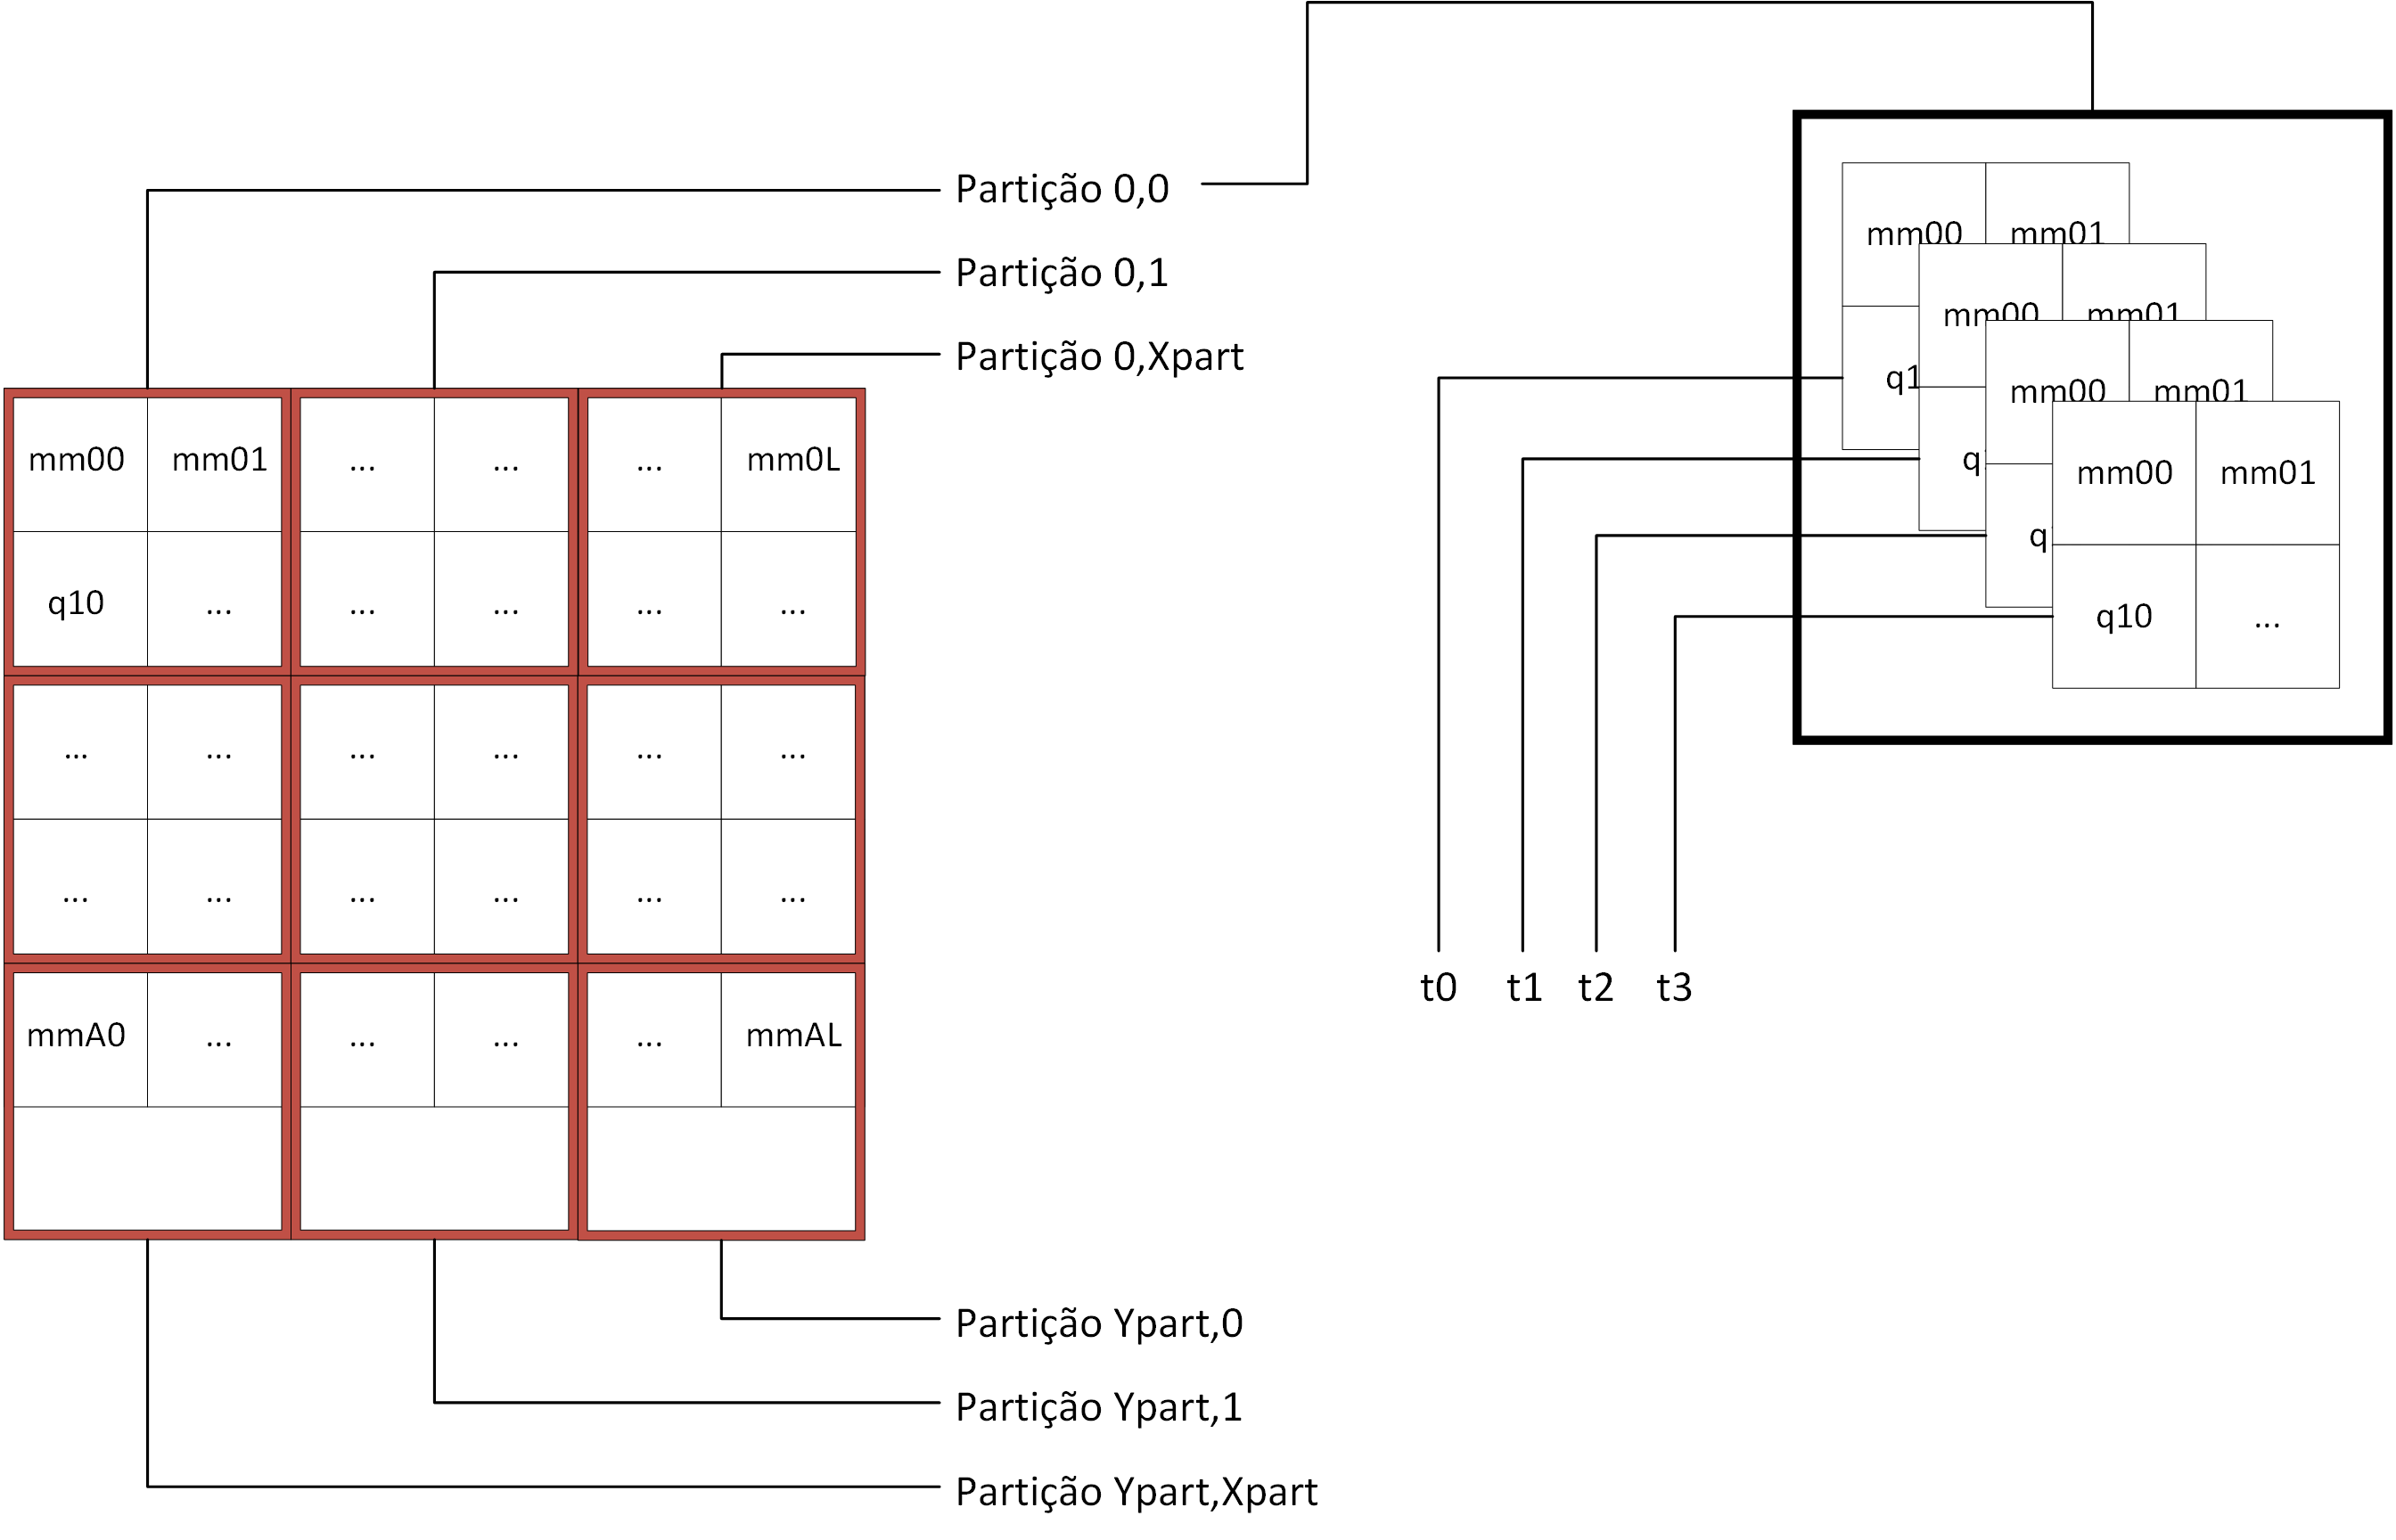
\includegraphics[scale=0.6]{Figuras/Ilustrations-PartitionedQuadricMap.png}
	\caption{Ilustração do mapa de quadrículas particionado.}
	\label{fig:PartitionedQuadricMap}
\end{figure}

Como mencionado nos parágrafos anteriores, este particionamento  é uma forma de fazer uma previsão sobre das pequenas regiões particionadas do mapa original, pois a operação de avaliação utilizada, é uma heurística que leva em consideração a operação de convolução sobre imagens, e neste caso, cada quadrícula está sendo representada por um pixel da imagem (mapa matriz) a ser operada pela convolução para gerar a previsão. Tal técnica será discutida mais adiante, mas já se adianta que a convolução tem a capacidade de  transformar uma matriz em outra, passando um filtro ou máscara de convolução sobre da matriz em questão, gerando uma matriz resultado. Caso se tente buscar um filtro de convolução para a matriz completa, englobam-se muitas características das áreas ou regiões mais influentes, e as regiões menos influentes serão ignorados. Isto resulta  apenas em um mapa que é a média da distribuição de carga geral por todo o mapa, e com um acúmulo de erro muito grande sobre os períodos, e que neste caso não nos interessa. Por este motivo é que foi feito o particionamento do mapa de modo que cada pequena região tenha destacada suas características principais a fim de fazer uma previsão mais precisa para todo mapa a partir da previsão das pequenas regiões. Este particionamento pode ser considerado um quadriculamento do mapa de quadrículas, o motivo pelo qual não se usa  uma quadrícula maior é que ela é usada segundo \citeauthor{willis2002spatial}  com seu tamanho original de aproximadamente \(\frac{1}{4} milha\),  e para este trabalho, foi usado um tamanho menor, uma vez que se deseja ter mais resolução nos dados para a adição deste a mais, que particiona o mapa de quadrículas em vários mapas menores. Assim cada  partição é um conjunto de quadrículas que representará uma imagem a ser processada pelo algoritmo, o qual buscará a melhor previsão desta pequena região.

Então, ao final do processamento não se terá apenas uma solução para previsão  total do mapa, mas sim várias soluções boas de previsão, para várias pequenas regiões, as quais irão compor o mapa final de previsão para a quantidade de períodos escolhida.

Para se criar as partições inicialmente define-se apenas dois valores, que representará quantas partições haverão no eixo das ordenadas \(Xpart\) e no eixo das abscissas \(Ypart\). Assim, calcula-se o total de partições como sendo \(Xpart \cdot Ypart\). No caso da figura \ref{fig:PartitionedQuadricMap}, \(Xpart\) e \(Ypart\) são iguais a 3. Assim como para o mapa final, cada partição será processada independente uma da outra, de modo que exista no final, uma previsão para cada partição dos mapas matrizes, as quais são reconstituídas em um único mapa matriz após todo o processamento para a apresentação do resultado final. Observe que como \(Xpart\) e \(Ypart\) são iguais a 3, cada partição tem o tamanho de 2, pois a regra de cálculo para o tamanho de cada partição a partir de \(Xpart\), \(Ypart\) segue a expressão \ref{eq:calcParts}:

\begin{equation}
\label{eq:calcParts}
\centering
\begin{split}
PartWidth = FLOOR(mapWidth / Xpart);\\
PartHeitht = FLOOR(mapHeight / Ypart);
\end{split}
\end{equation}

Calcula-se então os crescimentos absolutos para cada partição a fim de que este valor seja usado também pela função de avaliação que será utilizada no processo evolutivo, e armazena os valores em uma lista de vetores de crescimentos absolutos para cada partição. 

Conclui-se então, a modelagem do ambiente, demonstrando como os dados iniciais foram transformados até antes de serem processados para geração da previsão através do processo evolutivo, que neste caso será feita pelo algoritmo imperialista competitivo, com uma função de aptidão ou \emph{fitness} modelada utilizando os dados de uma lista de mapas matrizes particionado e os dados de crescimento absoluto nesta partição que serão descritos a seguir. Neste ponto os dados que aplicação possui carregados em memória são:
\begin{enumerate}
\item Mapa de quadrículas, carregado a partir dos arquivos gerados por seleção no banco de dados para cada período.
\item Vetor Multiplicador de Carga, definido de forma constante na aplicação. Para trabalhos futuros pode ser definido um multiplicador de carga para cada região particionada e seus valores podem ser definidos de acordo com algum algoritmo inteligente que processo os dados
\item Norte, Sul, Leste e Oeste, que são os limites em coordenadas que define a região da previsão.
\item Tamanho da quadrícula, Definido como descrito por \citeauthor{willis2002spatial}, com o valor de aproximadamente \(\frac{1}{4} milha\).
\item Vetor de períodos, não foi mencionado no texto mais quando se carrega os dados é criado um vetor contendo o valor de cada período apenas para impressão dos resultados  e definição dos períodos de treino e teste descritos posteriormente.
\item Vetor de períodos, não foi mencionado no texto mais quando se carrega os dados é criado um vetor contendo o valor de cada período apenas para impressão dos resultados  e definição dos períodos de treino e teste descritos posteriormente.
\item Uma lista de mapas matrizes, onde a quantidade de mapas matrizes presentes na lista é a quantidade de arquivos de períodos lidos no início da aplicação, e cada mapa matriz representa a densidade de carga em uma região durante o período que gerou este mapa matriz.
\item \(Xpart\) e \(Ypart\), que definem em quantas partições os mapas matrizes  serão quebrados para gerar uma previsão para cada conjunto de mapas matrizes de cada  uma destas partições.
\item Uma lista de mapas matrizes particionados, onde a quantidade de mapas matrizes particionados é igual a \(Xpart \cdot Ypart\),  e, para cada mapa matriz particionado será gerada uma previsão. 
\end{enumerate}


\section{Inicialização do ICA}

Para que o ICA seja inicializado apropriadamente, de forma a gerar soluções que possam ser usadas para prever a densidade espacial de carga períodos a frente, é necessário que se modele o problema como foi feito nos problemas \ref{G1Problem}G1 e G2\ref{G2Problem}, descritos no neste capítulo pelo item \ref{Exemplos de aplicação do ICA genérico}. Assim, é necessário que sejam definidos, a função de avaliação, o que cada dimensão representará durante o processo evolutivo, e consequentemente a quantidade de dimensões. Deve-se também antes de iniciar o processo evolutivo definir quais são os limites de cada dimensão definida.

A modelagem do problema da previsão da densidade espacial de carga para otimização pelo ICA, se resume em uma implementação da interface \emph{IFitness}, de forma que tal implementação seja capaz de evoluir os valores, ou atributos, dos indivíduos, a fim de que a melhor solução possa ser aplicada na base de dados para se gerar previsões. Observa-se que para obter uma previsão sobre os dados é necessário utilizar o ICA para evoluir os indivíduos até um período antes do que se deseja gerar a previsão (sobre dados históricos, em forma dos mapas matrizes particionados), e então utilizar os indivíduos evoluídos junto deste último período, passando-os pela função de previsão usada durante a avaliação, a fim de gerar uma previsão para o próximo período. Para fazer a previsão de mais de um período à frente, basta utilizar o resultado obtido da previsão do período anterior e executar novamente a função de previsão, que irá gerar desta vez uma previsão sobre um período já previsto, acumulando assim o erro de previsão inicial (base inicial \(\Rightarrow\) previsão1) e o erro de previsão atual (previsão1 \(\Rightarrow\) previsão2). Quanto mais períodos forem previstos mais erro acumulado será gerado nas previsões futuras.

A técnica utilizada para fazer com que os elementos do ICA possam evoluir, e fornecer as melhores soluções, tal que quando aplicadas sobre os dados para períodos futuros, devem fornecer previsões espaciais da região selecionada. Assim  entende-se que a função avaliação deve ser dependente do tempo, e este tempo, será definido como o número de períodos selecionados para o problema, por serem espaçados igualmente. Porém a intenção não é fazer uma previsão de crescimento para cada quadrícula presente no mapa, uma vez que a intenção é buscar também a influência que os vizinhos aplicam sobre a quadrícula, elaborando assim, uma técnica que leva em consideração uma quantidade de quadrículas, de modo que se defina um padrão de crescimento médio, relativo tanto ao crescimento do ponto quanto à evolução da forma da região em questão. Tendo assim, no final, um mapa que forme regiões de maior possibilidade de ocorrência de aumento de densidade para os períodos futuros.

Tem-se que o mapa é representado como uma imagem através dos mapas matrizes para cada período, então foi elaborada uma técnica  semelhante a técnica apresentada no problema G2 \ref{G2Problem}, a qual buscará pela melhor solução, de forma que se encontrem os melhores filtros ou matrizes de convolução,porém, neste caso,  ponderados de acordo com suas relevâncias, tal que estes filtros quando aplicados na matriz de um período \(t0\) opere gerando uma nova matriz \(t1’\), que seja mais semelhante possível à matriz do período \(t1\), e quando aplicada à matriz do período \(t1\), opere gerando uma nova matriz \(t2’\), que seja mais semelhante possível ao período \(t2\), e assim por diante.

Um grande problema, não apenas para este tipo de solução, mas para todas as técnicas de previsão, é a previsão futura que leva em consideração muitos períodos a frente, e que utilizam-se dos períodos anteriores para prever o novo período, é  referente ao grande acúmulo de erro durante a previsão para estes períodos futuros mais distantes da origem.Então sabe-se que a previsão tem um bom resultado para os períodos iniciais e acumulará mais erro para os períodos futuros. Entretanto, insere-se um fator na avaliação a fim de fazer com que as matrizes ou filtros de convolução, durante a evolução, levem em consideração a taxa de crescimento média daquela região, o que ajuda a diminuir um pouco deste erro, e faz com que a solução tenha uma tendência para o crescimento médio desta região.


\subsection{Avaliação dos países}

A avaliação do problema deve fornecer indivíduos capazes de efetuar uma previsão de densidade espacial, sobre a região apresentada, para um ou mais períodos à frente, a partir de um conjunto de mapas matrizes e os índices de crescimento absoluto durante os períodos. Assim, a avaliação de cada indivíduo irá ser resumida nas etapas:
\begin{itemize}
\item Tradução do vetor de atributos dos países;
\item Processamento dos mapas de previsão; 
\item Cálculo parcial do erro;
\item Avaliação dos erros e atribuição do custo;
\end{itemize}

A tradução do vetor de atributos basicamente transforma o vetor de atributos do de um dado país, em estruturas mais práticas para o processamento, tal que o acesso ao vetor de atributos seja minimizada e o gerenciamento dos elementos sejam simplificados, gerando assim, um vetor de valores unitários, contendo os valores de ponderação, e um vetor de filtros, ou máscaras, do mesmo tamanho do vetor anterior, contendo matrizes que representam os filtros que serão usados para a convolução.   

O processamento dos mapas de previsão é a parte principal da avaliação, e é responsável por reproduzir o processo de previsão sobre os mapas matrizes existentes, o qual será usado para efetuar a previsão real, assim que o ICA terminar a competição imperialista, fornecendo o melhor país como solução. Esta etapa então, itera por todos os mapas matrizes, com exceção do último, utilizando as máscaras de convolução, transformadas do vetor de atributos do país, para gerar mapas que sejam o resultado da convolução entre o mapa matriz do período em questão com as matrizes de convolução provindas de cada ponderação, gerando assim vários mapas matrizes. A partir destes mapas resultantes, gera-se então um mapa ponderado, sendo este a ponderação dos mapas resultantes da convolução, onde os fatores de ponderação são os contidos no vetor de valores unitários de ponderações, traduzido dos atributos dos países. Assim, com este mapa final ponderado dos diversos mapas de convolução, gera-se um mapa final que é o resultado da soma do mapa deste período com o mapa ponderado, sendo este mapa final o mapa previsto para o período seguinte, \(t_1’\), sendo \(t_0\) o período atual. 

Antes mesmo de sair da iteração principal, pelos mapas matrizes, calcula-se a diferença entre o mapa de previsão e o mapa real do próximo período, e tais diferenças são usadas então, para gerar os erros produzidos em cada iteração. O cálculo dos erros leva em conta ainda o crescimento absoluto que cada período tem para com o seu próximo, então, se a diferença pode ser calculada como mostra expressão\ref{eq:forecastdif}:

\begin{equation}
\label{eq:forecastdif}
dif = ABS( Mapa[t_1] - Mapa[t_1’] ).
\end{equation}
	
Para se calcular o erro total gerado durante este período, levando em consideração o mapa de previsão e o crescimento em relação ao período de forma igualitária, fazendo-se a multiplicação da diferença \(dif\) por \(0.5\), e então soma-se com o valor de crescimento absoluto entre os períodos \(t_x\) e \(t_{x+1}\), que também é multiplicado por \(0.5\). Sendo assim, este valor final de erro para o dado período \(t_x\), ou iteração atual,é armazenado em um vetor de erros \(Errors\) que armazenará todos os erros gerados a durante cada iteração entre os períodos em que se fará a previsão, como mostra a expressão \ref{forecastError}:

\begin{equation}
\label{eq:forecastError}
	Errors[t_x] = dif \cdot 0.5 + CrescimentoAbsoluto[t_x \Rightarrow t_{x+1}] \cdot 0.5.
\end{equation}

	A utilização do crescimento absoluto na função de avaliação poderia ser removida, que o resultado seria algo muito parecido se não o mesmo, porém este fator é inserido para que o processo evolutivo chegue mais rapidamente ao resultado esperado, de modo que tal influência acelere e refine o resultado final do país. Por fim, durante a última e mais simples etapa, somam-se todos os erros e atribui ao valor de custo do país em questão, finalizando assim a avaliação de um indivíduo. 

Este processo de avaliação faz com que o país, ao longo das eras tenha seus atributos convergindo para a melhor solução, operando a convolução e ponderando os mapas matrizes tal que o erro gerado pelo mapa de previsão seja o mais próximo do mapa real e também, tal que seu crescimento seja predito de acordo com o crescimento entre os períodos reais. 

A ponderação entre os mapas de convolução, ao invés de apenas usar uma operação de convolução diretamente, sem ponderação, é necessária para que o mapa final resulte em uma previsão mais exata. Pois entende-se que ao tentar buscar uma matriz de convolução entre duas imagens, as quais uma é o resultado da passagem da matriz de convolução sobre a outra, como descrito no problema G2 \ref{G2Problem}, é um problema diferente do objetivo do trabalho, o qual é mais simples, apesar da complexidade da solução, por se saber que existe, de fato, um filtro ou matriz de convolução que leva uma imagem ser transformada em outra, quando operada a convolução. Já o problema proposto, a diferença entre um período e outro não é apenas a busca por uma matriz de convolução, mas sim a previsão, que para isto, são usadas matrizes de convolução com seus resultados ponderados, onde cada uma destas matrizes de convolução agrega uma ou mais características da região durante um dado período, que são relevadas pelo fator de ponderação. Observa-se que o problema proposto ainda utiliza as mesmas matrizes de convolução para operar por todos os períodos, então se houverem várias características que possam vir a ser identificadas durante todos os períodos, as matrizes terão mais liberdade de adaptação, sendo que tais características podem variar entre as máscaras de convolução e ser ponderadas de acordo com suas relevâncias. Observa-se ainda, que a intenção não é obter o resultado exato, mas sim uma matriz que gere um mapa semelhante que possa ser usado para previsão futura das regiões.

A figura \ref{fig:ForecastEvalPart0}  ilustra uma situação de avaliação para cinco períodos, \(t0\), \(t1\), \(t2\), \(t3\) e \(t4\), tais que máscaras de convolução, \(Masks 1,2,...,n\), geram mapas matrizes, \(t1’(1,2,...,n)\), \(t2’(1,2,...,n)\), \(t3’(1,2,...,n)\) e \(t4’(1,2,...,n)\), que são ponderados para gerar mapas de previsão, \(T1’\), \(T2’\), \(T3’\) e \(T4’\).

\begin{figure}[h]
	\centering	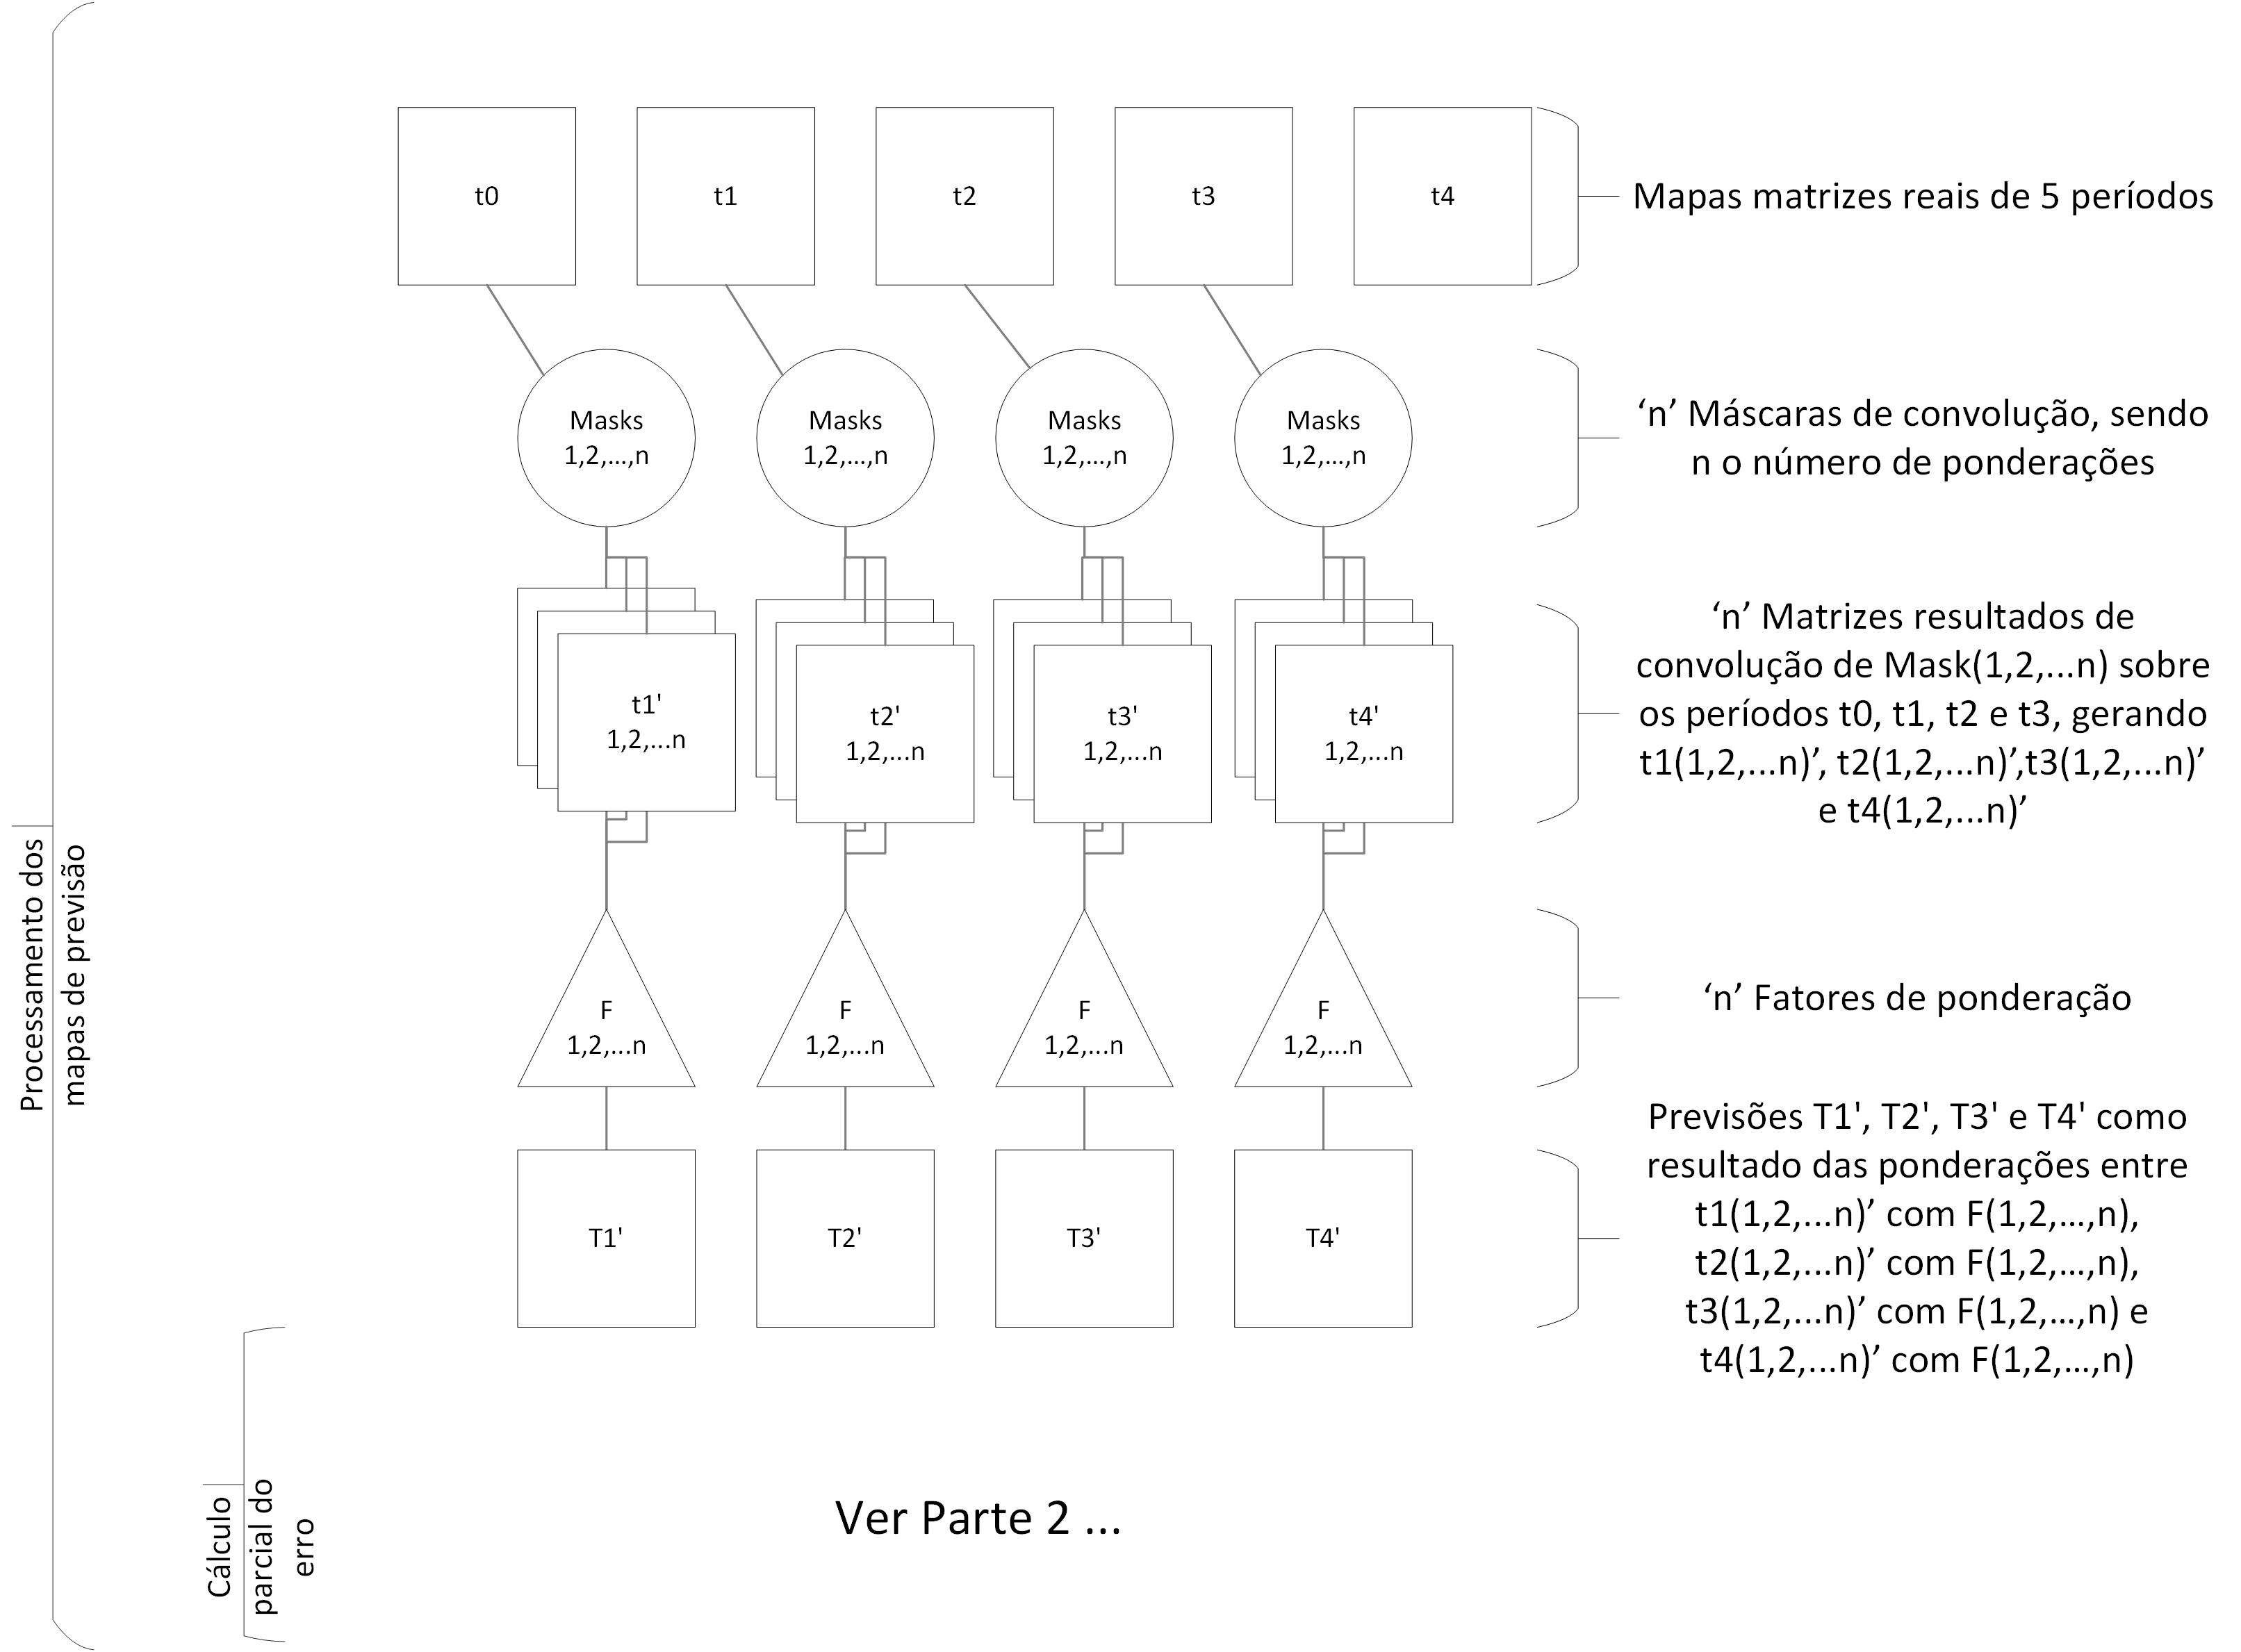
\includegraphics[scale=0.55]{Figuras/Ilustrations-ForecastEvalPart0.png}
	\caption{Processamento dos mapas de previsão parte 1.}
	\label{fig:ForecastEvalPart0}
\end{figure}

Já a figura \ref{fig:ForecastEvalPart1}  mostra como os cálculos parciais são executados, sendo que faz-se o uso dos mapas matrizes de previsão e dos mapas matrizes reais tal que se tenha no final, armazenados no vetor \emph{resultValues}, os erros gerados de modo que este vetor possa ser usado para que se atribua o custo do país na próxima etapa. de avaliação dos erros e atribuição do custo.

\begin{figure}[h]
	\centering	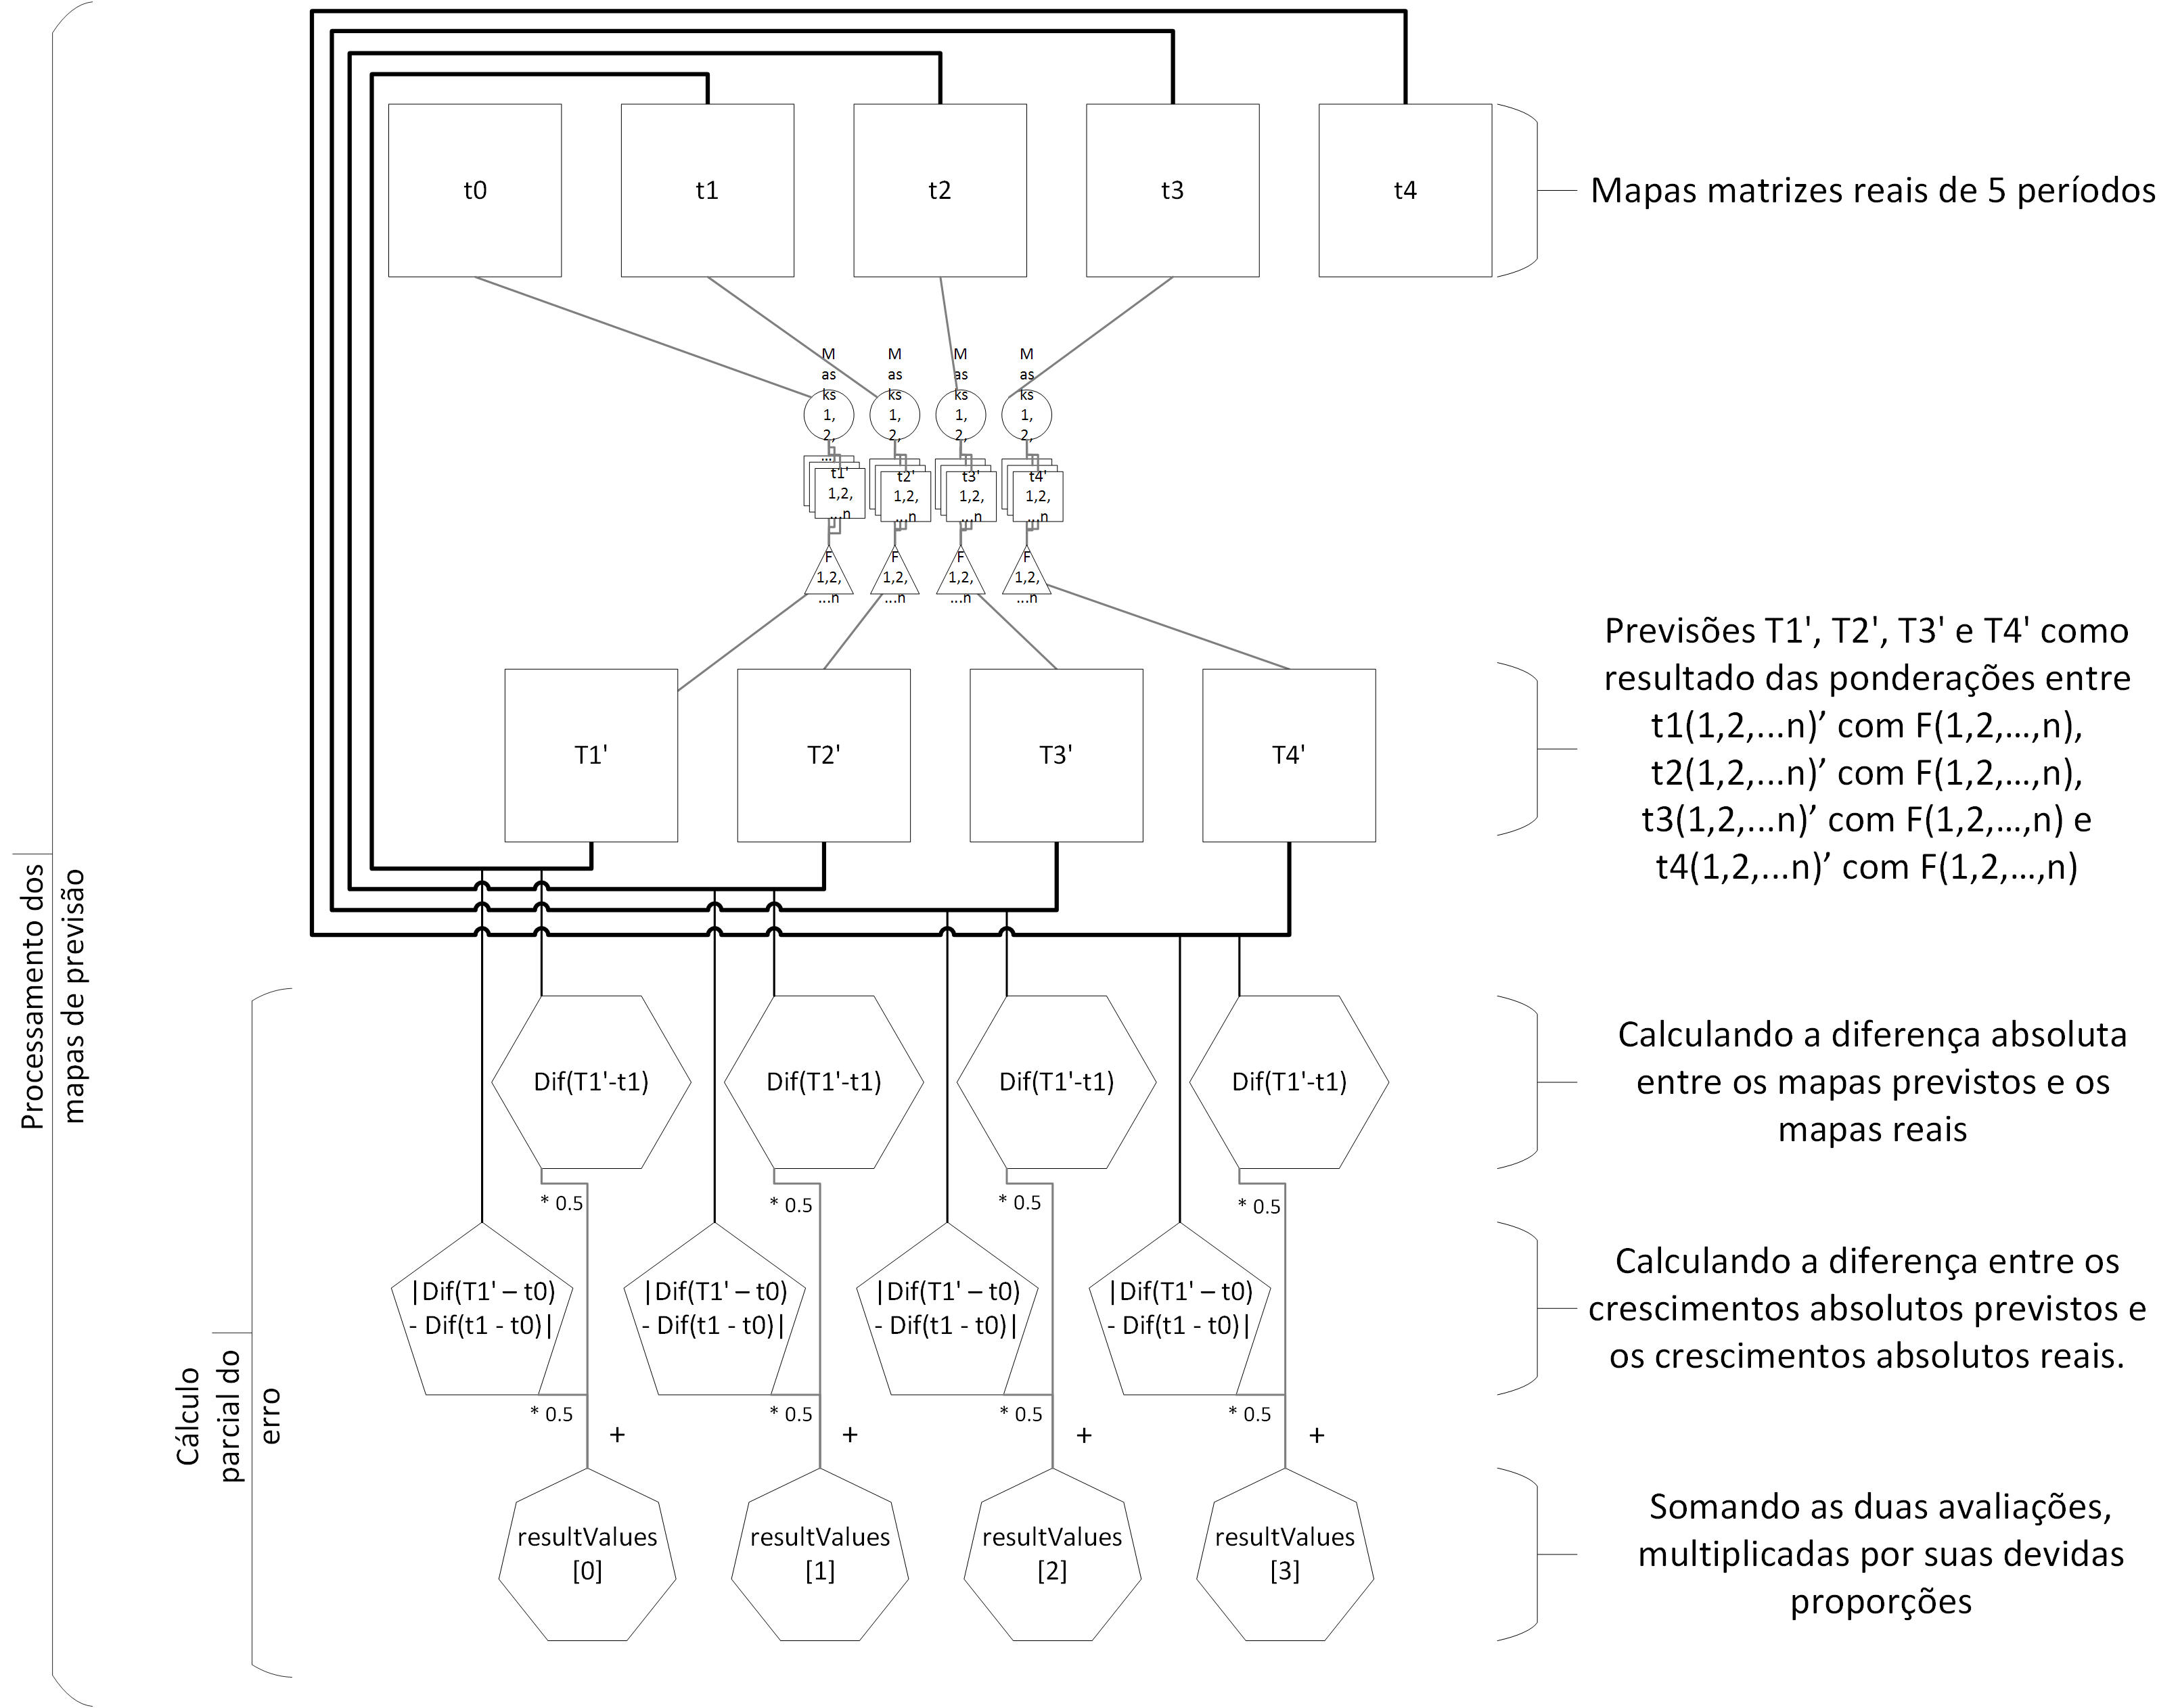
\includegraphics[scale=0.55]{Figuras/Ilustrations-ForecastEvalPart1.png}
	\caption{Processamento dos mapas de previsão parte 2.}
	\label{fig:ForecastEvalPart1}
\end{figure}

Assim, resumidamente o que ocorre no processamento dos mapas de previsão durante a evolução, é a utilização de todos os períodos para uma forma de treinamento dos países competidores no ICA tal que estes sejam capazes, quando aplicados a um dado período, de produzirem um período à frente do período utilizado, como mostra a expressão:

\begin{equation}
\label{eq:forecastError}
Mapa(t_1’) = F(Mapa(t_0), País)
\end{equation}

De modo que durante as próximas etapas, sejam calculados os erros, comparando o mapa de previsão gerado em \(Mapa(t_1’)\) com o mapa real do período \(Mapa(t_1)\), tanto em semelhança quanto em crescimento absoluto. Atribuindo assim este erro como sendo o custo do país, a fim de se obter um país, para que o ICA, então, retome seu processo evolutivo, que decidirá através das operações já mencionadas se este país possui atributos melhores que os demais, terminando assim a etapa de avaliação dos países, que ocorre muitas vezes até que se chegue em um resultado otimizado, o qual satisfaça as condições de parada.




\subsection{A função de avaliação}

A primeira etapa da implementação da função de avaliação, que é definida pelo problema em questão, para ser processado pelo ICA, é a definição da interface \emph{IFitness} e consequente implementação de seus métodos e propriedades em uma classe chamada \emph{PonderationFullConvolutionFitness}. A implementação desta interface, independente da implementação dos métodos ou propriedades, divide-se nas partes: 
\begin{itemize}
\item Definição de constantes e inicialização das constantes;
\item Definição do método de inicialização dos países;
\item Definição da função de avaliação e
Teste.
\end{itemize}

Começando então pela definição dos valores constantes e suas inicializações, para este problema é interessante manter uma cópia da lista de mapas matrizes, denominada \emph{MapsList}, em cache, de modo que esta lista possa ser acessada por múltiplas tarefas em paralelo (provindo de chamadas feitas paralelamente pelo ICA), evitando que haja escrita, pois o modelo utilizado para representar esta lista é seguro e não obstrutivo (\emph{Thread Safe}) apenas para leitura de dados da lista. Outros dois valores constantes que definem o vetor de atributos do país são:
\begin{itemize}
\item \emph{PonderationCount}, que define o número de ponderações e consequentemente quantas matrizes de convolução existirão;
\item \emph{Order}, que define qual será a ordem das matrizes de convolução. 
\item \emph{absoluteGrowths}, que define o crescimento absoluto entre os mapas matrizes período a período, sendo este valor calculado assim que se entra com os mapas matrizes na lista de mapas \emph{MapsList}.
\item \emph{maskCount}, que representa a quantidade de valores presente em cada máscara, utilizado para a definição do número de dimensões e durante a tradução da lista de atributos. 
\end{itemize}

Observe que estes dois últimos elementos poderiam não existir, porém, para que possa se otimizar a função de avaliação, que pode ser chamada milhares de vezes, calculam-se todos estes elementos independentes, evitando cálculos desnecessários durante as chamadas de avaliação.

O método de inicialização dos países é bem simples, uma vez que não insere dados de entrada nos atributos dos países e o problema não exigiu alteração das funcionalidades básicas do país. Assim, a inicialização dos países se resume na criação de uma lista de países do tamanho \emph{Dimensions}, que gera \emph{nPopulation} países com atributos uniformemente aleatórios, onde cada dimensão está limitada entre \emph{minBounds} e \emph{maxBounds}. Os valores \emph{nPopulation}, \emph{minBounds} e \emph{maxBounds} são parâmetros de entrada da função recebidos diretamente do ICA, os quais podem ser configurados antes de se chamar o método \emph{Run()} do ICA que evolui os países. Já o valor de \emph{Dimensions} é um cálculo que utiliza os valores definidos anteriormente e é definido a seguir,  em \ref{Atributos dos Países}, mostrando o que cada atributo presente nos países representa no problema e como eles são traduzidos para serem utilizados pela função de avaliação.





\subsubsection{Atributos dos Países}
\label{Atributos dos Países}

A partir da ideia gerada durante a modelagem da função de avaliação, definiu-se como deve ser modelado um país para que o ICA processe este problema e quais são os componentes do vetor de atributos a serem evoluídos durante a competição. Então como será feita uma ponderação de matrizes de convolução, em \emph{PonderationCount}, tem-se quantas ponderações devem ser feitas, em \emph{Order}, qual a ordem das matrizes de convolução. Assim, o número de atributos total que os países do ICA terão, definido em \emph{Dimensions}, na implementação do objeto que contém a função de avaliação, pode ser descrito como apresentado na expressão \ref{eq:forecastDimensions}: 
	
\begin{equation}
\label{eq:forecastDimensions}
\begin{split}
Dimensions = PonderationCount \cdot (maskCount + 1), 
\\\text{Onde}
\\maskCount = order \cdot order.
\end{split}
\end{equation}

A definição do valor de dimensões dos países é obrigatória e ocorre durante a inicialização do objeto que implementa a função de  avaliação (ou implementação da interface \emph{IFitness}), e faz parte da modelagem do problema. Note que não se define diretamente o valor de dimensões no país, mas sim na função de avaliação, para  que a solução fique genérica e dependa apenas da implementação da função de aptidão como demonstrado no capítulo de desenvolvimentoREFREFREFREFREFREFREFREFREFREFREFREFREFREFREFREFREFREFREFREFREFREFREFREFREFREFREFREFREFREFREFREF, e ainda, não se insere um valor fixo, mas sim na expressão \ref{eq:forecastDimensions} de modo que o número de dimensões ainda varie de acordo com os valores de número de ponderações e ordem da máscara de convolução.

	Cada país usa a implementação padrão da classe \emph{Country} do ICA, descrita no capítulo de desenvolvimentoREFREFREFREFREFREFREFREFREFREFREFREFREFREFREFREFREFREFREFREFREFREFREFREFREFREFREFREFREFREFREFREF, sem nenhuma alteração, assim, todo indivíduo terá uma distribuição uniforme quando gerar os números aleatórios para seus atributos, tanto em sua inicialização quanto em chamadas que sorteiam estes atributos do indivíduo durante a evolução, causadas pela operação de revolução colonial.

	A figura \ref{fig:VetorAtributosForecast-Ingles} ilustra como os valores são dispostos no vetor de atributos do país. Observe que primeiro vem o valor de ponderação e em seguida vem os valores da máscara de convolução, formando um bloco. O número de blocos é dependente da quantidade de ponderações que se deseja gerar para um mapa, e o tamanho de cada bloco depende da ordem da matriz de convolução.

\begin{figure}[h]
	\centering	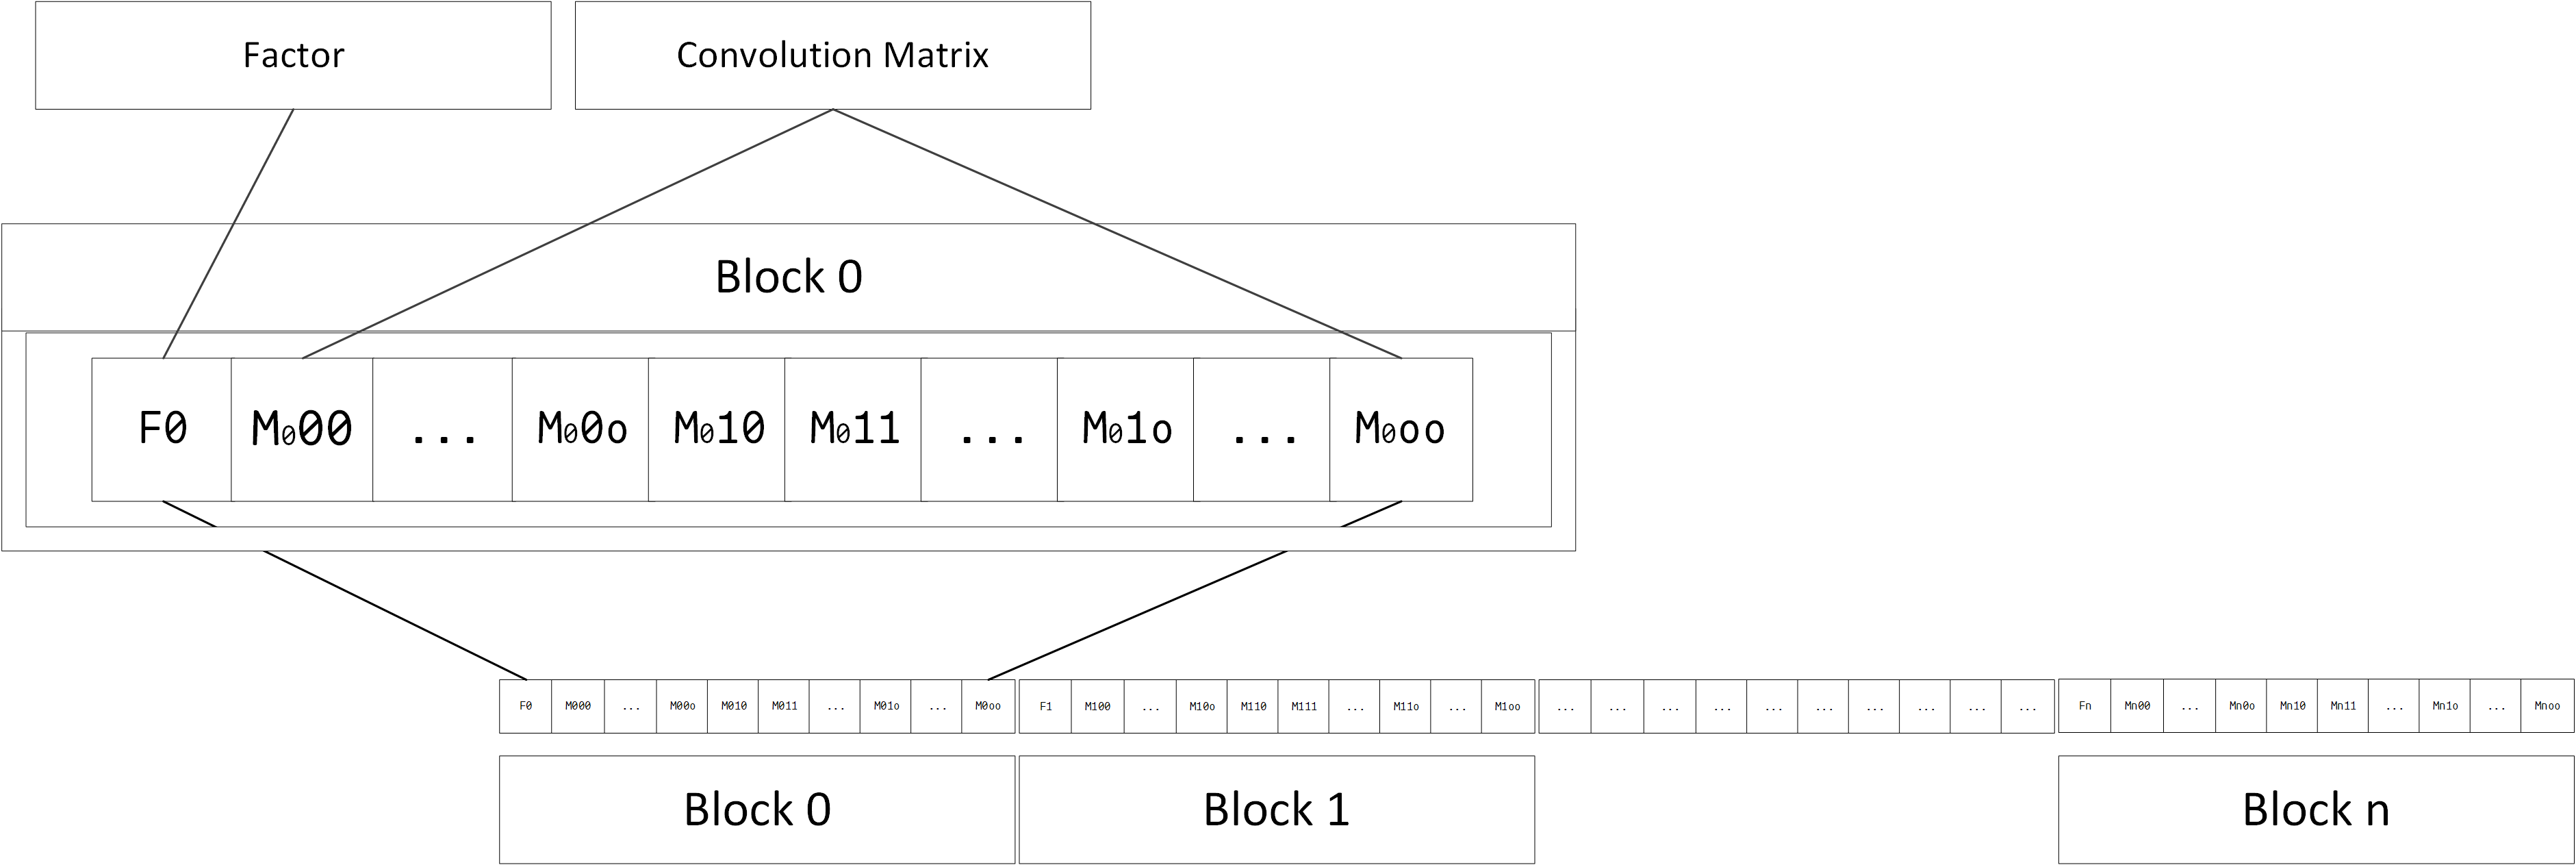
\includegraphics[scale=0.45]{Figuras/VetorAtributosForecast-Ingles.png}
	\caption{Vetor de atributos do país.}
	\label{fig:VetorAtributosForecast-Ingles}
\end{figure}


\subsection{Implementando a Função de Avaliação}
\label{Implementando a Função de Avaliação}

Voltando então para a implementação da função de avaliação, com o número de dimensões e a estrutura do vetor de atributos dos países já definidos, pode-se então, definir a implementação da função de avaliação em três partes como descrita anteriormente, porém agora mais resumidamente e com foco na implementação de cada item:

\begin{itemize}
\item Tradução do vetor de atributos dos países;
\item Processamento dos mapas de previsão 
\begin{itemize}
\item Cálculo parcial do erro;
\end{itemize}
\item Avaliação dos erros e atribuição do custo;
\end{itemize}

A tradução do vetor de atributos deve gerar dois elementos, o vetor de ponderações e o vetor de máscaras. Ambos são obtidos em um mesmo bloco que itera \emph{i} de 0 até o número de ponderações \emph{PonderationCount}. Assim o vetor de ponderações é preenchido como \ref{eq:forecastPonderation}:
	
\begin{equation}
\label{eq:forecastPonderation}
\begin{split}
ponderations[i] = element.Attributes[ponderationIndex];\\
\text{Sendo}\\
ponderationIndex = i \cdot (maskCount + 1);
\end{split}
\end{equation}


Em \ref{eq:forecastPonderation} ocorre uma cópia do valor contido no vetor de atributos no índice \emph{ponderationIndex} para o índice \emph{i} do vetor \emph{ponderations}.

E em seguida, utilizando-se deste índice de ponderações \emph{ponderationIndex}, copiam-se um intervalo de valores do vetor de atributos do país, de modo que esta cópia comece no índice \emph{ponderationIndex + 1} deste valor de atributos, que representa o primeiro elemento da máscara, e copie os valores até se atingir uma quantidade de elementos igual a \emph{maskCount}, tendo assim, um vetor de elementos que represente a máscara. Ainda não se tem portanto, a máscara no formato de uma matriz, então chama-se uma função externa para converter um vetor unidimensional de valores para uma matriz que represente uma máscara ou filtro de convolução, respeitando a ordem da máscara, como mostra o exemplo contendo o algoritmo \ref{alg:CountryTransform} usado em tal transformação:

\vspace{10px}
\begin{algorithm}[h]
\SetAlgoLined
\KwData{
\\ Atributos - [1, 2, 3, 4, 5, 6, 7, 8, 9].
\\ Ordem - 3.
}
\KwResult{ 

\\Máscara\\
[1, 2, 3]\\
[4, 5, 6]\\
[7, 8, 9]

}
inicializar a matriz \emph{masks[Ordem][Ordem]} com zeros\;

\For{$k \leftarrow $0 \KwTo $Ordem*Ordem$}
{
\tcp{índice x é o resto da divisão de k por ordem.}
x = k \% Ordem\;
\tcp{índice y.}
y = (k - x ) / Ordem\;
mask[x][y] = Atributos[k]\; 
}
\caption{ Algoritmo Transformação do vetor de atributos do país.}
\label{alg:CountryTransform}
\end{algorithm}

Após a obtenção da máscara representada pela estrutura matricial, que é então adicionada em um vetor de matrizes chamado \emph{ponderationMasks}, termina-se a etapa de tradução do vetor de atributos do país para dois vetores, \emph{ponderations} e \emph{ponderationMasks}, contendo os valores de ponderação e as máscaras de convolução usadas para gerar os mapas de ponderação respectivamente.

Seguindo, para a etapa de processamento dos mapas de previsão, diversas inicializações são feitas, na ordem:
\begin{enumerate}
\item Inicializar o vetor de valores resultados em \emph{resultValues}.
\item Inicializar o vetor de imagens resultado da operação de ponderação entre as matrizes de convolução em \emph{ponderationImages}.
\item Inicializar o vetor de mapas resultantes da convolução em \emph{resultMaps}
\item Inicializar uma matriz para representar o mapa final gerado dos processos de convolução e ponderação, para posterior comparação e cálculo do erro.
\end{enumerate}



Após estas atualizações, itera-se por todos os mapas com exceção do último, gerando os mapas de convolução de cada período, no vetor \emph{resultMaps}, mapeando o resultado do cálculo para um mapa ponderado, na matriz \emph{result} , e gerando então, um mapa final, \emph{finalResult}, de previsão do próximo período ao se somar o mapa do período atual. E, por fim, comparando  ambos, o mapa real do próximo período e o mapa final de previsão processado, a fim de gerar os erros e armazená-los no vetor \emph{resultValues} para posterior definição de custo do país, conforme mostra o algoritmo:

\vspace{10px}
\begin{algorithm}[h]
\SetAlgoLined
\KwData
{
\\ \emph{PonderationCount} - número de ponderações.
\\ \emph{TrainingSize} - quantidade de períodos para treino.
\\ \emph{height} - altura em quadrículas da região.
\\ \emph{width} - largura em quadrículas da região.
\\ \emph{MapList} - Lista de mapas históricos de quadrículas.
\\ \emph{masks} - vetor de máscaras de convolução.
\\ \emph{ponderations} - vetor de fatores de ponderação. 
}
\KwResult{ \\ cost - custo avaliado do país. }

next = 1\;
\tcp{Iteração de previsão.}
\For{$now \leftarrow $0 \KwTo $TrainingSize - 1$}
{
\tcp{Início da função de previsão.}
	\For{$i \leftarrow $0 \KwTo $PonderationCount$}
    {
    	resultMaps[i] = Convolution(MapList[now].MapMatrix, masks[i])\;
    }
    result = new Matrix[width][height]\;
    \For{$x \leftarrow $0 \KwTo $width$}
    {
    	\For{$y \leftarrow $0 \KwTo $height$}
        {
          num = 0; den = 0\;
          \For{$i \leftarrow $0 \KwTo $PonderationCount$}
          {
			num += resultMaps[i].MapMatrix[x][y] * ponderations[i]\;
            den += resultMaps[i].MapMatrix[x][y]\;
          }
          result[x][y] = num / den\;
        }
    }
    finalResult = Sum(MapList[now].MapMatrix, result)\;
    \tcp{End Of Fp function.}
    resultValues[now] = Diference(MapList[next].MapMatrix, finalResult) * 0.5 + Abs(Diference(MapList[now].MapMatrix, finalResult) - absoluteGrowths[now]) * 0.5\;
    next = now + 1;
}
cost = resultValues.Sum()\;
\caption{ Avaliação do país.}
\label{alg:CountryEval}
\end{algorithm}

Na linha 1 inicia-se o valor de iteração para o índice do próximo período em \emph{next}. Na linha 2 inicia-se o processo de treino do país, passando por todos os períodos exceto o último, de forma que se itere o valor \emph{now}, que representa o período atual, até um período antes do último. Em seguida, nas linhas 3 e 4, geram-se todos os mapas de convolução, referentes a cada ponderação, baseando-se no mapa matriz do período definido por \emph{now}. A linha 6 apenas inicializa um mapa vazio com as mesmas dimensões dos mapas matrizes dos períodos. Então, nas linhas 7 e 8, inicia-se o processo de iteração por todas as quadrículas (ou pixels) do mapa matriz, usando \emph{x} para deslocamento pela largura e \emph{y} pela altura. Em 10, 11, 12 calcula-se a soma dos numeradores e denominadores das ponderações de cada mapa multiplicado pelo valor de ponderação, gerando assim, um valor ponderado para cada pixel dentre cada um dos mapas de ponderações. Deste modo, atribui-se ao pixel \(\left(x,y\right)\) na matriz resultado, o valor ponderado \emph{result[x][y]}, sendo o numerador dividido pelo denominador calculado no passo anterior usando os valores de ponderação como base de cálculo. Para a obtenção do mapa final de previsão na linha 17, adiciona-se o mapa resultado ao mapa base do período, sendo que tal mapa final represente o mapa futuro como sendo o mapa atual somado com os valores de desvio gerados da ponderação das convoluções de cada pixel. Por fim, na linha 18, ocorre a atribuição do valor de erro gerado pela previsão deste período para o vetor \emph{resultValues}, sendo esta a parte mais crítica, que define de fato se a previsão feita é semelhante ao esperado ou não.

Observa-se que o cálculo dos valores \emph{resultValues} são ponderados com \(0.5\) e \(0.5\), o que indica que ambos os valores têm mesmo peso para a avaliação. Caso fosse utilizado \(0.75\) para a previsão e \(0.25\) para os valores absolutos, teria-se uma avaliação que 'prefere’ que o país tenha suas matrizes de convolução e fatores de ponderação se caracterizando mais nos mapas matrizes reais do que levando em consideração os crescimentos absolutos entre os períodos previstos e reais. 

Em seguida, os erros acumulados no vetor \emph{resultValue}, referentes cada um a uma iteração pelos períodos, comparando-os ao período seguinte, devem ser somados e então atribuídos como custo do país, terminando assim a avaliação do país, como:

\[Country.Cost = Sum(resultValues);\]

As funções \emph{Abs}, \emph{Sum}, \emph{Diference} e \emph{Convolution}, são funções, chamadas externamente, que operam valores, vetores ou, matrizes, tal que:
\begin{itemize}
\item \emph{Abs} recebe um valor numérico e retorna o valor absoluto deste número.
\item \emph{Sum} tem duas sobrecargas, sendo
\begin{itemize}
\item a primeira, tendo como entrada um vetor de valores e retorna a soma entre todos os valores deste vetor.
\item e a segunda, tem como entrada duas matrizes de largura e altura iguais e retorna como resultado uma nova matriz, com altura e largura também iguais as matrizes de entrada, onde esta matriz resultado representa a soma dos elementos de cada índice das matrizes de entrada.
\end{itemize}
\item \emph{Diference} tem como entrada duas matrizes de altura e largura iguais, onde será calculada e retornada a diferença total e absoluta entre os os elementos de cada índice das matrizes de entrada.
\item \emph{Convolution} é uma operação mais complexa, que executa a convolução de um filtro ou matriz de convolução sobre uma matriz, ambos passados como parâmetro, e neste caso, ignora-se os valores de ajuste(\emph{offset}) e divisor (citados nos conceitos de convolução) são mantidos nulos, valendo respectivamente 0 e 1, uma vez que o ICA já se encarrega de configurar apropriadamente os índices da matriz, como se ela já possuísse os valores de ajuste e divisor aplicados a si.
\end{itemize}








\subsection{A ponderação das matrizes de convolução}
\label{A ponderação das matrizes de convolução}

A ponderação se faz importante porque neste caso, as partições dos mapas que representam os períodos subsequentes, não necessariamente são o resultado da convolução de uma máscara pela região do mapa do período anterior. Então, deve-se estimar a média de crescimento da região através de um fator, porém o objetivo não é obter o crescimento homogêneo de toda uma região, mas sim obter um crescimento direcionado não homogêneo e relativo tanto aos valores de cada quadrícula quanto aos valores das quadrículas vizinhas. Assim gera-se no final, um mapa com maior resolução, que sofre influência e aplica influência sobre seus vizinhos, demonstrando o crescimento regional num mapa bidimensional, sem que seja necessário calcular regiões as tendências ponto a ponto, o qual levaria a apenas um crescimento calculado estatisticamente para aquele ponto apenas, sem levar em consideração seus pontos vizinhos.

A figura \ref{fig:MapaMatrizT0} apresenta um exemplo de como esta técnica de ponderações age sobre uma matriz de valores representando uma região de \(10x10\) quadrículas (ou \emph{pixels}), que está prestes a ser ponderada. O exemplo abaixo apresenta valores totalmente aleatórios para as máscaras e fatores de ponderação, como se fossem o primeiro cálculo durante o treinamento, tendo como intenção a demonstração detalhada da mecânica deste processo de ponderação. Durante o processo evolutivo espera-se que tanto os fatores quanto as máscaras de convolução tenham seus valores ajustados para o mais similar possível do mapa do próximo período. 

\begin{figure}[h]
	\centering	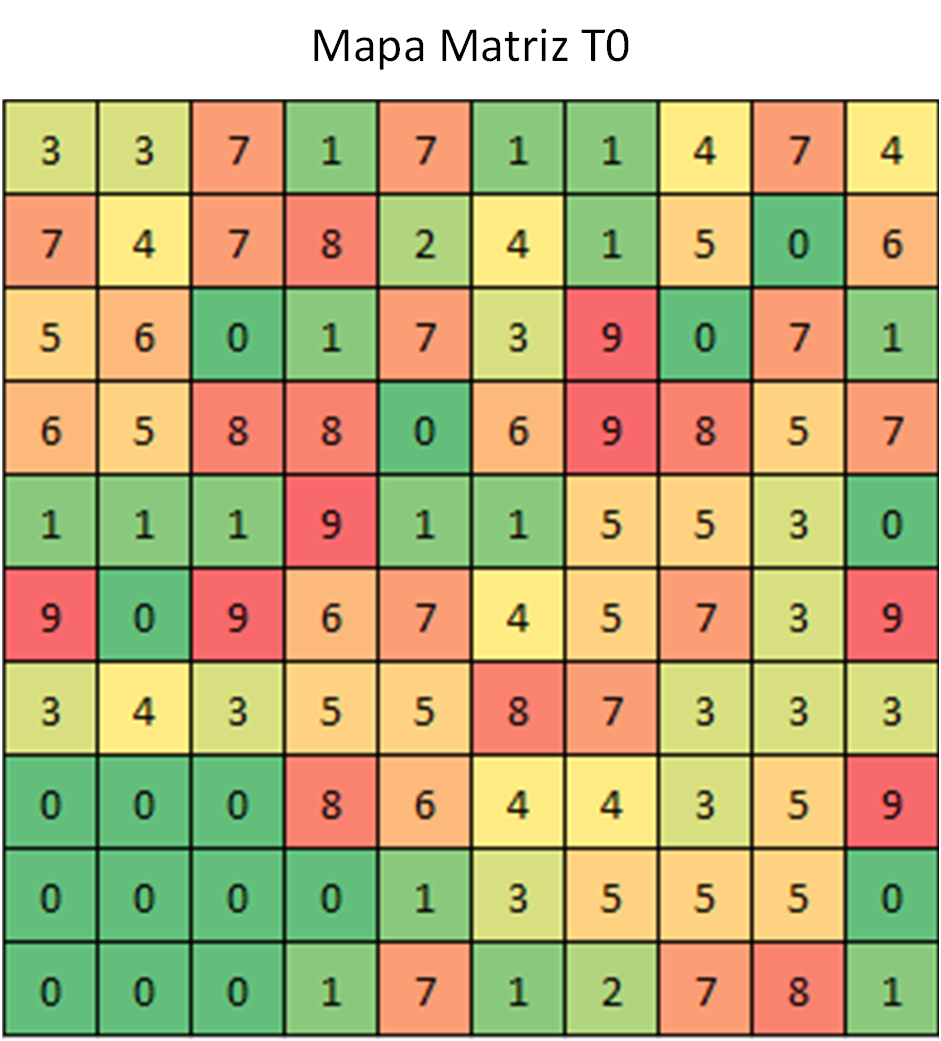
\includegraphics[scale=0.6]{Figuras/PonderationsExample-MatrixMap.png}
\caption{Exemplo de ponderação - MapaMatriz T0.}
\label{fig:MapaMatrizT0}
\end{figure}

Na figura \ref{fig:OnePondertion} pode-se observar que foi escolhido apenas um fator de ponderação, o que fez com que a operação de convolução se torne completamente inútil, não sendo necessário seu cálculo, pois o fator aplicará como resultado do cálculo de apenas uma ponderação um crescimento homogêneo por quase todo o mapa, por exemplo, para um ponto qualquer \((x,y)\), este deve ser calculado na matriz de ponderação como:

\begin{equation}
\label{eq:ponderation1}
\begin{split}
Ponderação(x,y) = \sum_{i=0}^{PonderationCount} \left(\frac{Convolution(x,y) \cdot Fator[i]}{Convolution(x,y)}\right)
\end{split}
\end{equation}

Assim o ponto (0,0) seria:

\[Pond1(0,0) = \frac{Convolution(0,0) \cdot Fator1}{ Convolution(0,0)};\]
\[Pond1(0,0) = \frac{141 \cdot 0,5}{ 141 } = 0,5;\]


\begin{figure}[h]
	\centering	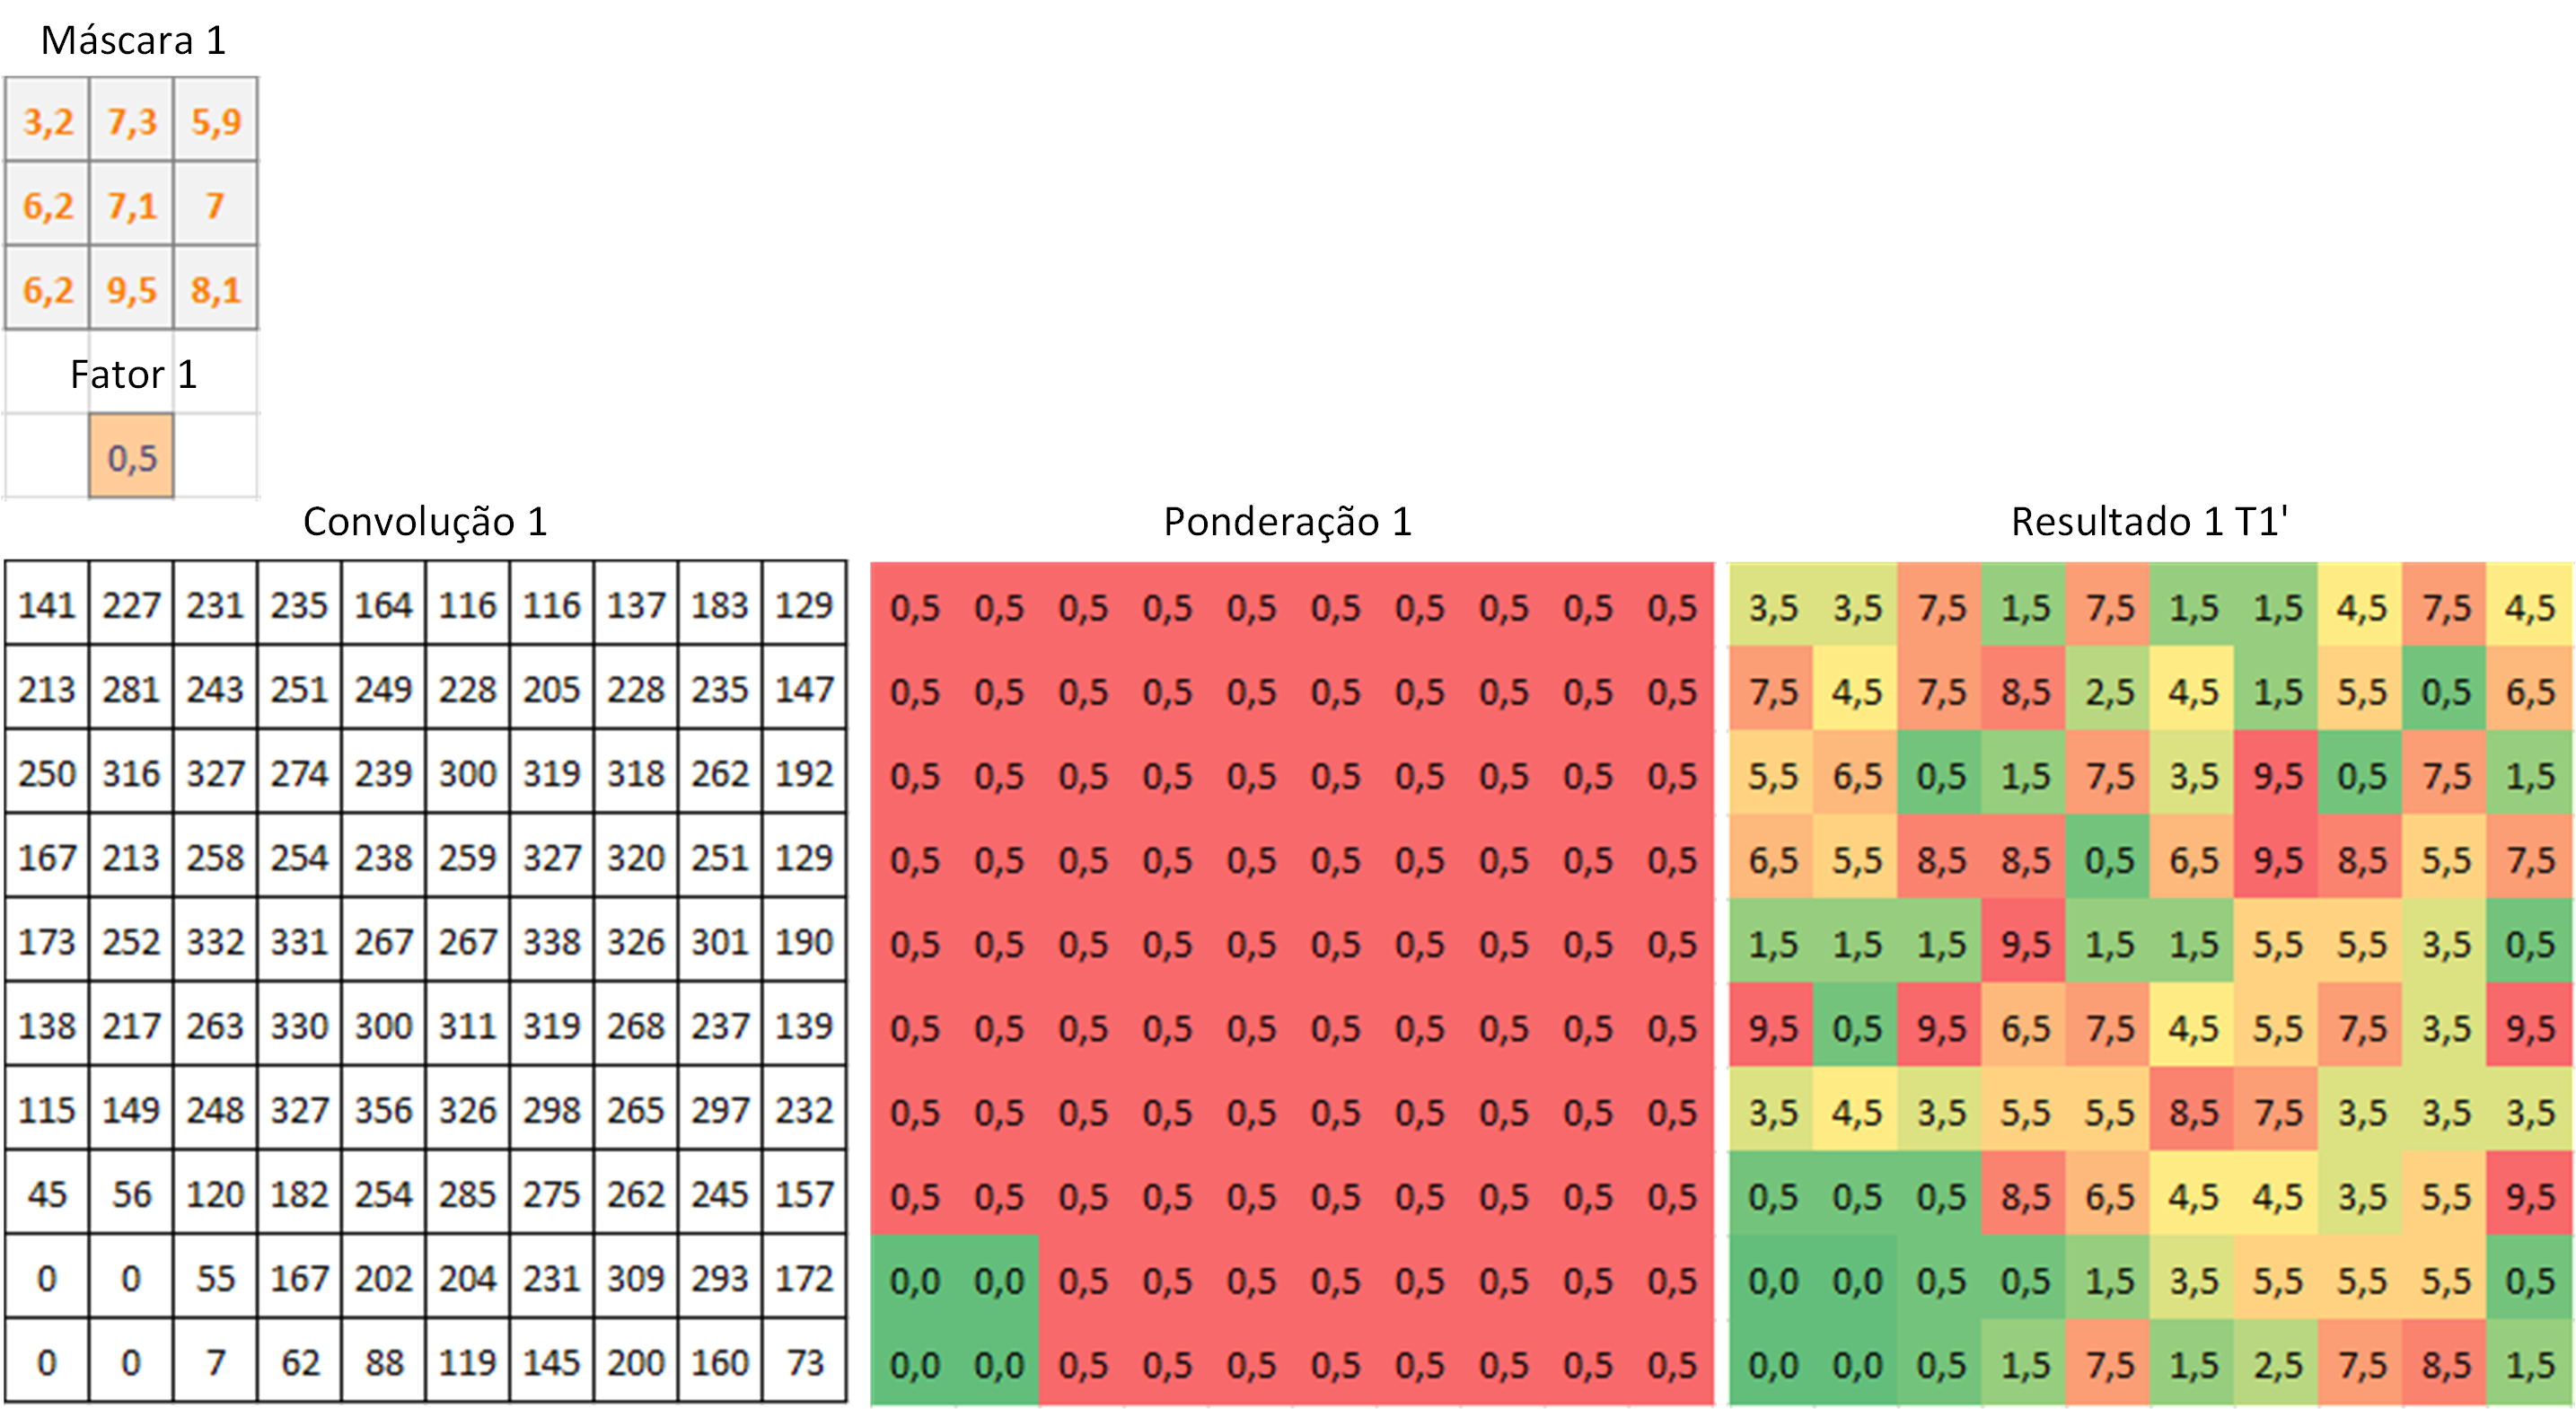
\includegraphics[scale=0.6]{Figuras/PonderationsExample-1Ponderation.png}
	\caption{Exemplo de ponderação - 1 ponderação}
	\label{fig:OnePondertion}
\end{figure}

Observe que se houver apenas uma ponderação o processo evolutivo tenderá ao crescimento médio da região durante os períodos, que neste caso levaria a uma previsão similar às apresentadas por técnicas estatísticas que usam a linha de tendência de crescimento aplicadas ponto a ponto, neste caso região por região. Ainda assim, este método demonstra um crescimento que expande ao longo dos períodos, pois no canto inferior esquerdo, houve expansão de 1 quadrícula sobre os valores que antes eram nulos. A matriz Resultado \emph{T1} é basicamente a soma ponto a ponto da matriz Ponderação 1 com o Mapa Matriz T0 (da figura \ref{fig:MapaMatrizT0}).

Ao se adicionar mais um fator de ponderação, como mostra a figura \ref{fig:TwoPondertion}, já é possível notar que o mapa de ponderação gerado não é mais homogêneo como o anterior, e que os cálculos de cada ponto do mapa de ponderações leva em consideração o valor de seus vizinhos. E ainda, o mapa \emph{Resultado 2} \emph{T1’} apresenta-se muito semelhante ao mapa anterior, crescendo não homogeneamente nesta região. A matriz \emph{Ponderação 2} segue o mesmo cálculo apresentado em \ref{eq:ponderation1}, usando as matrizes \emph{Convolução 1} (da figura \ref{fig:OnePondertion}) e \emph{Convolução 2} (da figura \ref{fig:TwoPondertion})

\begin{figure}[h]
	\centering	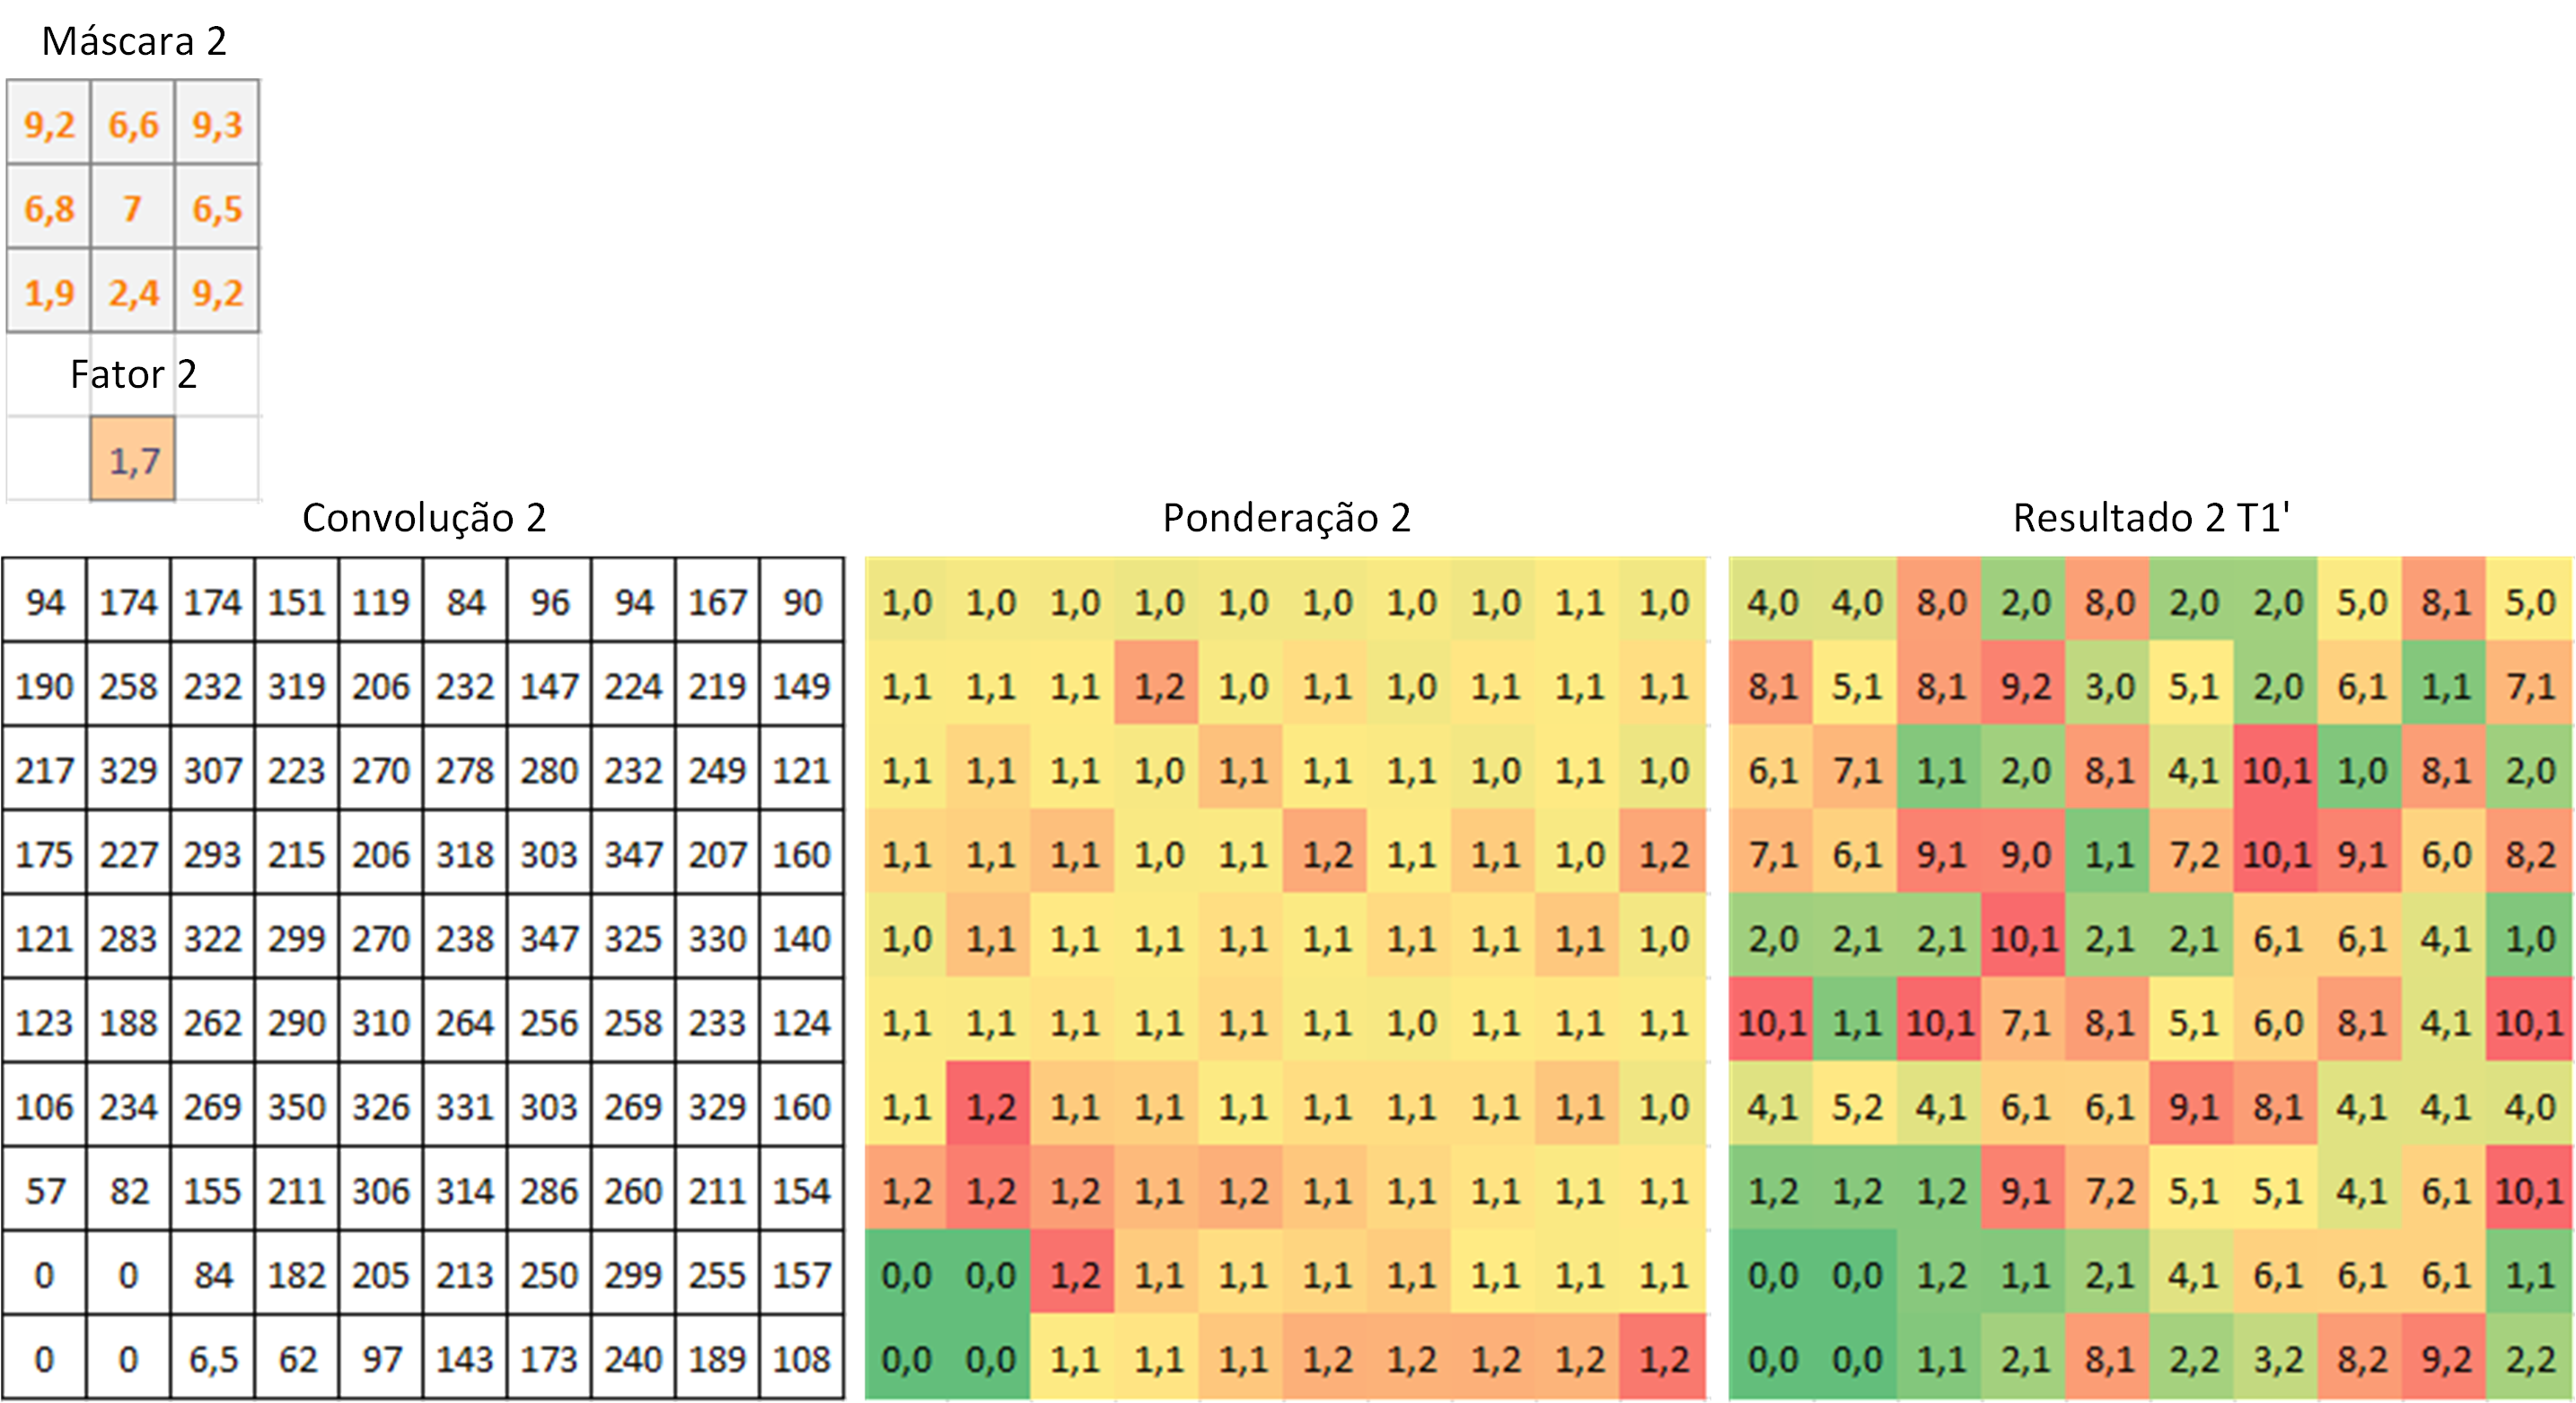
\includegraphics[scale=0.6]{Figuras/PonderationsExample-2Ponderations.png}
	\caption{Exemplo de ponderação - 2 ponderações}
	\label{fig:TwoPondertion}
\end{figure}
 
	Por fim, a figura \ref{fig:TreePondertion}, aumenta-se o número de ponderações para 3, o que consequentemente leva a 3 fatores de ponderação com a necessidade do cálculo de 3 matrizes de convolução e geração aleatória de 3 máscaras de convolução. Neste caso, observa-se que o fator apresenta um valor negativo, que decresce todo o crescimento do mapa mas mantém um padrão de crescimento muito similar ao anterior (apresentado pela figura\ref{fig:TwoPondertion}). 
    
\begin{figure}[h]
	\centering	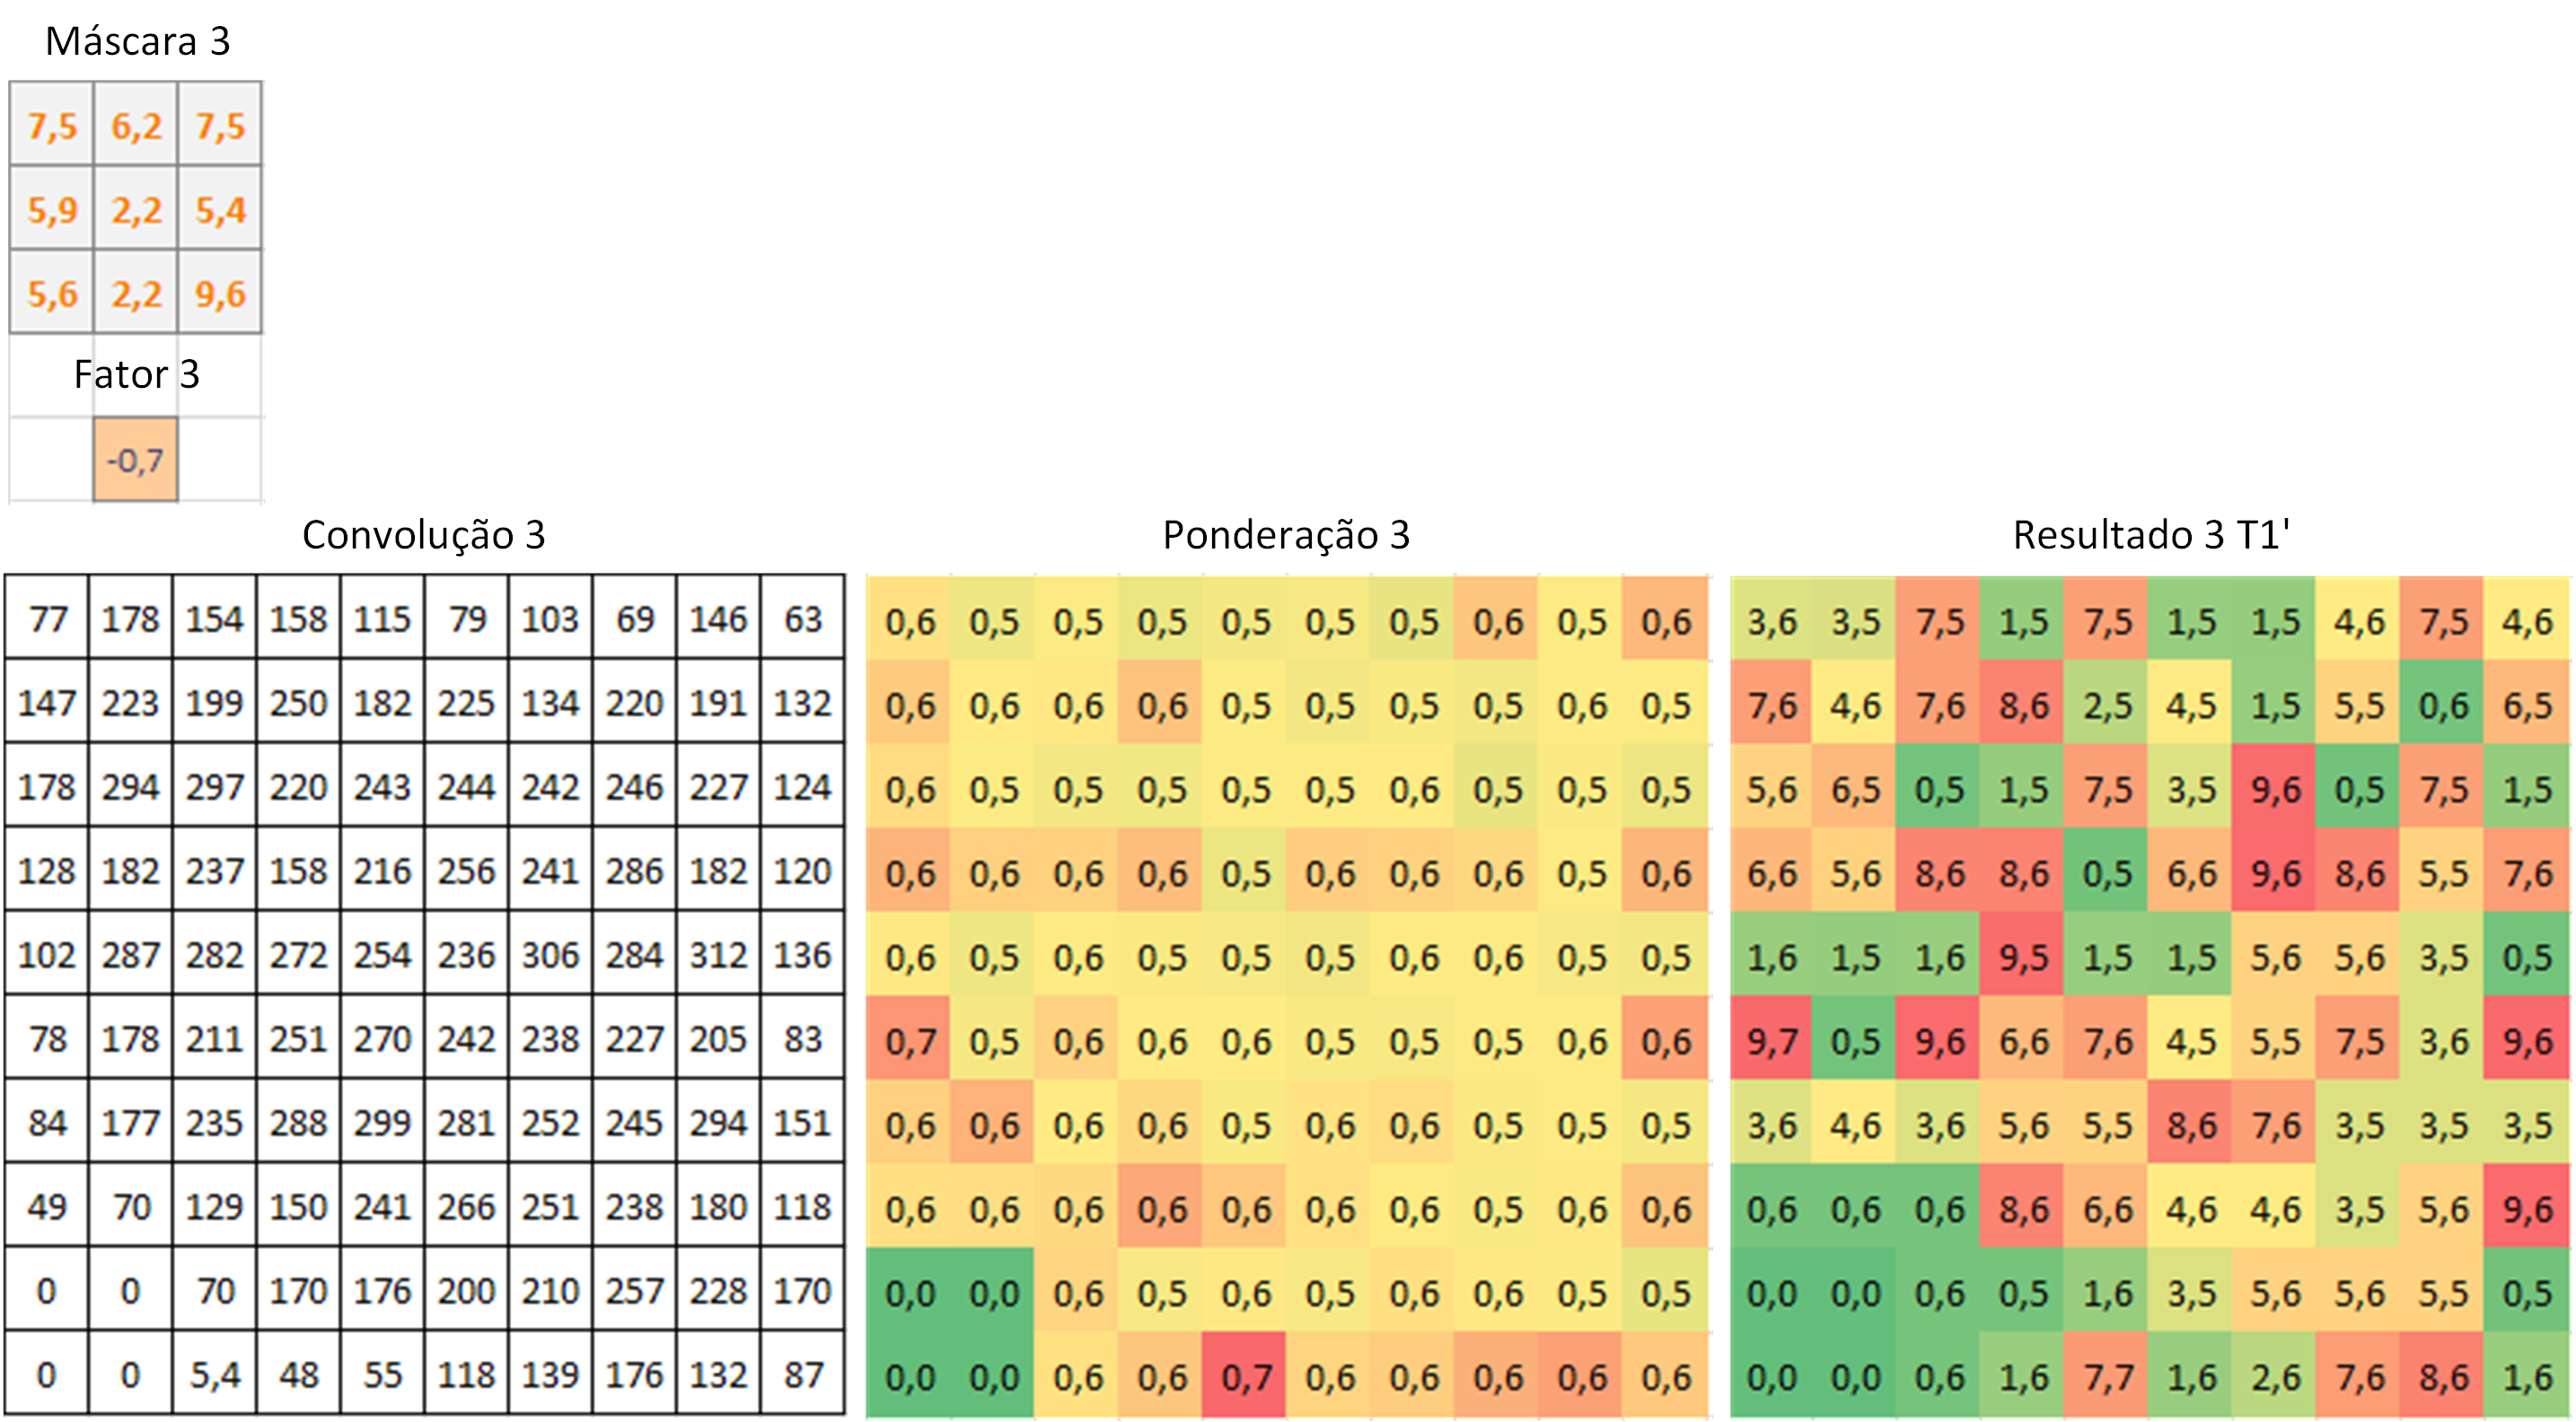
\includegraphics[scale=0.6]{Figuras/PonderationsExample-3Ponderations.png}
	\caption{Exemplo de ponderação - 3 ponderações}
	\label{fig:TreePondertion}
\end{figure}

Neste caso, com três ponderações, é possível notar que os valores dos fatores de ponderação geram valores para os pontos tal que estes serão diferentes porém com uma tendência à média dos fatores, e também são limitados na soma dos fatores. O que proporciona esta diferenciação entre os valores são as matrizes de convolução, que são usadas como ajuste, de modo que cada máscara gere uma matriz que releve uma ou mais características do mapa a ser ponderada, com o fator, neste caso, fazendo o papel de relevar ou não a característica em questão. 

Assim, é possível notar, que neste caso totalmente aleatório já existe uma tendência de crescimento geral, onde algumas regiões crescem mais que outras, de forma não homogênea, definida por características do mapa do período base, podendo assim, repetir-se tal processo para que tal tendência seja aplicada novamente sobre o mapa Resultado gerado, a fim de gerar uma previsão futura de um próximo período seguindo esta mesma tendência de crescimento. 

Espera-se então, que ao fim do processo evolutivo, ao aplicar esta técnica, que leva como parâmetros o conjunto de valores compostos por máscaras e fatores, seja possível gerar uma previsão tendenciosa, ou seja, que segue a curva de tendência de crescimento para a região, de forma não homogênea, ressaltando pontos de maior e menor crescimento dependentes de características adquiridas pelos ajustes dos valores, principalmente dos valores das máscaras de convolução, e por fim de forma apresentável bidimensionalmente, de modo que tal região venha compor o mapa final. 

\subsection{A Etapa de Previsão}
\label{A Etapa de Previsão}

Voltando o foco agora para a mecânica do ICA, a avaliação ocorre para todos os indivíduos na mesma etapa, podendo ser processada em serial ou em paralelo. Observe que a avaliação de cada indivíduo ocorre independente dos demais, de modo que todo recurso compartilhado não restrinja o uso apenas para aquela avaliação, possibilitando assim que o processamento das avaliações dos países possa ser executado em tarefas paralelas paralelas. Assim que todas as avaliações são finalizadas, independente de terem ocorrido paralela ou serialmente, o ICA passa para as próximas etapas que, então irão alterar todas as características dos países até que se termine a iteração e entre novamente na etapa de avaliação, onde todos os indivíduos são novamente avaliados. A condição de parada padrão geralmente é o número máximo de décadas, que quando atingida, termina a evolução dos indivíduos e consequentemente da competição imperialista. 

Assim que a competição termina e o método `Run` acaba sua execução retornando para o escopo da aplicação, é possível então pegar qualquer país usado na competição imperialista, e utilizá-lo para aplicar tal solução ao problema. O interessante é utilizar o país de menor custo, uma vez que esta é a melhor solução buscada pelo ICA. Assim, este melhor indivíduo é usado na etapa de teste, que, neste caso, é aplicado para gerar mapas de previsão de períodos futuros através de um processo muito semelhante ao processo feito pela função de avaliação. No processo de avaliação, iterou-se por diversos períodos gerando um mapa de previsão para cada período. No caso da etapa de testes, não se faz tal iteração, apenas executa-se o processo de geração do mapa de previsão, que basicamente faz os processos:

\begin{itemize}
\item Tradução do vetor de atributos do país.
\item Processamento de um mapas de previsão a partir do último período usado.
\end{itemize}

O processo de tradução do vetor de atributos do país já fora detalhado anteriormente e não muda em nada durante esta etapa de testes. O processamento de um mapa de previsão deve sempre ocorrer a partir do último mapa usado na etapa de avaliação, sendo este o ano base para que se gere as demais previsões. Este processo de testes sempre irá gerar um período de previsão a frente do período passado, então para se gerar mais de um período de previsão, é necessário executar este processo tantas vezes quanto se queira ter previsões de períodos futuros, passando como parâmetro, um mapa para previsão e um país, para se gerar um segundo que é o resultado do processo de previsão por usando o método de convoluções ponderadas, como mostra o algoritmo \ref{alg:Fp}:

\begin{algorithm}[h]
\SetAlgoLined
\KwData
{
\\ \emph{PonderationCount} - número de ponderações.
\\ \emph{Map} - o mapa base, que terá previsão de 1 período à frente.
\\ \emph{height} - altura em quadrículas da região.
\\ \emph{width} - largura em quadrículas da região.
\\ \emph{masks} - vetor de máscaras de convolução.
\\ \emph{ponderations} - vetor de fatores de ponderação. 
}
\KwResult{ \\ finalResult - como o mapa de previsão de 1 período à frente de Map. }
 
	\For{$i \leftarrow $0 \KwTo $PonderationCount$}
  {
   	resultMaps[i] = Convolution(Map.MapMatrix, masks[i])\;
    }
     result = new Matrix[width][height]\;
     \For{$x \leftarrow $0 \KwTo $width$}
     {
     	\For{$y \leftarrow $0 \KwTo $height$}
         {
           num = 0; den = 0\;
           \For{$i \leftarrow $0 \KwTo $PonderationCount$}
           {
 			num += resultMaps[i].MapMatrix[x][y] * ponderations[i]\;
             den += resultMaps[i].MapMatrix[x][y]\;
           }
           result[x][y] = num / den\;
         }
     }
     finalResult = Sum(Map.MapMatrix, result)\;
   
 \caption{Algoritmo função de previsão}
\label{alg:Fp}
\end{algorithm}

Observe que o algoritmo é uma cópia de uma parte da função de avaliação, que gera o mapa de previsão de apenas um período, fazendo a soma de todos os mapas operado-os pela convolução e ponderando-os em um mapa final. Assim, como mencionado anteriormente, é possível gerar várias previsões, utilizando o mapa gerado de uma previsão t1` para se prever t2` e assim por diante. Porém, como a previsão de um segundo período é sobre uma previsão já feita, acumulam-se os erros de previsões, aumentando drasticamente a incerteza para previsões mais futuras.


